\documentclass[11pt,letterpaper]{book}
\setlength{\oddsidemargin}{0.5in}
\setlength{\topmargin}{0in}
\setlength{\evensidemargin}{0.3in}
\setlength{\textwidth}{5.75in}
\setlength{\textheight}{8.5in}
%\setlength{\oddsidemargin}{1.25in}
%\setlength{\evensidemargin}{0.5in}

% don't do this \usepackage{times}    % Better fonts than Computer Modern
%\usepackage{times}
\renewcommand{\sfdefault}{phv}
\renewcommand{\rmdefault}{ptm}
% don't replace tt -- old is better \renewcommand{\ttdefault}{pcr}
%\usepackage{apalike}
%\usepackage{pslatex}
\usepackage{techref}
\usepackage{epsfig}
\usepackage{verbatim}
\usepackage{moreverb}
\usepackage{graphicx}
\usepackage{xspace}
\usepackage{multicol}
\usepackage{color}
\usepackage{html}
\usepackage{array}
\usepackage{multirow}
\usepackage{longtable}
%\usepackage{version}
\usepackage{makeidx}
%\usepackage{showidx}
\usepackage[chapter]{algorithm}
\floatname{algorithm}{Listing}

\usepackage{syntax}

\usepackage{fancyhdr}
\pagestyle{fancy}
\fancyhead[LE,RO]{\bfseries\thepage}
\fancyhead[LO]{\bfseries\rightmark}
\fancyhead[RE]{\bfseries\leftmark}
\fancyfoot[C]{\bfseries OpenImageIO Programmer's Documentation}
\renewcommand{\footrulewidth}{1pt}


\def\product{{\sffamily OpenImageIO}\xspace}
\def\OpenImageIO{{\sffamily OpenImageIO}\xspace}
\def\versionnumber{1.3}
\def\productver{\product\ {\sffamily \versionnumber}\xspace}
\def\producthome{{\codefont \$IMAGEIOHOME}\xspace}
\def\ivbinary{{\codefont iv}\xspace}
\def\maketx{{\codefont maketx}\xspace}
\def\iconvert{{\codefont iconvert}\xspace}
\def\idiff{{\codefont idiff}\xspace}
\def\iinfo{{\codefont iinfo}\xspace}
\def\igrep{{\codefont igrep}\xspace}
\def\oiiotool{{\codefont oiiotool}\xspace}
\def\ImageSpec{{\codefont ImageSpec}\xspace}
\def\ImageInput{{\codefont ImageInput}\xspace}
\def\ImageOutput{{\codefont ImageOutput}\xspace}
\def\ParamBaseType{{\codefont ParamBaseType}\xspace}
\def\TypeDesc{{\codefont TypeDesc}\xspace}
\def\ParamValue{{\codefont ParamValue}\xspace}
\def\ParamValueList{{\codefont ParamValueList}\xspace}
\def\ImageBuf{{\codefont ImageBuf}\xspace}
\def\ImageCache{{\codefont ImageCache}\xspace}
\def\TextureSystem{{\codefont TextureSystem}\xspace}
\def\ROI{{\codefont ROI}\xspace}
\def\IBA{{\codefont ImageBufAlgo}\xspace}
\def\NULL{{\codefont NULL}\xspace}
%\def\opencall{{\codefont open()}\xspace}
\def\writeimage{{\codefont write\_image()}\xspace}
\def\writescanline{{\codefont write\_scanline()}\xspace}
\def\writetile{{\codefont write\_tile()}\xspace}
\def\readimage{{\codefont read\_image()}\xspace}
\def\readscanline{{\codefont read\_scanline()}\xspace}
\def\readtile{{\codefont read\_tile()}\xspace}
\def\AutoStride{{\codefont AutoStride}\xspace}


\title{ 
{\Huge{\bf \product}
%\textregistered\ 
{\bf\sffamily \versionnumber} \medskip \\ \huge Programmer Documentation
\\ \large (in progress) 
} \bigskip }
\author{Editor: Larry Gritz \\
\emph{lg@openimageio.org}
 \bigskip \\
}
\date{{\large 
%Editor: Larry Gritz \\[2ex]
Date: 24 Sep 2013
%\\ (with corrections, 4 Aug 2013)
}}


%%%%%%%%%%%%%%%%%%%%%%%%%%%%%%%%%%%%%%%%%%%%%%%%%%%%%%%%%%%%%%%%%%%%%%%%%%
% Larry's favorite LaTeX macros for making technical books.  These have
% been refined for years, starting with SIGGRAPH course notes in the
% '90's, further refined for _Advanced RenderMan_.
%%%%%%%%%%%%%%%%%%%%%%%%%%%%%%%%%%%%%%%%%%%%%%%%%%%%%%%%%%%%%%%%%%%%%%%%%%

%
% Define typesetting commands for filenames and code
%
% Just like Advanced RenderMan -- all code in courier, keywords in text
%    courier but not bold.
\def\codefont{\ttfamily}	% font to use for code
\def\ce{\codefont\bfseries}	% emphasize something in code


%
% Define typesetting commands for filenames and code
%
\def\cf{\codefont}		% abbreviation for \codefont
\def\fn{\codefont}		% in-line filenames & unix commands
\def\kw{\codefont}      	% in-line keyword

\newcommand{\var}[1]{{\kw \emph{#1}}}  % variable
\newcommand{\qkw}[1]{{\kw "#1"}}       % quoted keyword
\newcommand{\qkws}[1]{{\small \kw "#1"}}       % quoted keyword, small
\newcommand{\qkwf}[1]{{\footnotesize \kw "#1"}}       % quoted keyword, tiny



% Define some environments for easy typesetting of small amounts of
% code.  These are mostly just wrappers around verbatim, but the
% different varieties also change font sizes.
\newenvironment{code}{\small \verbatimtab}{\endverbatimtab}
\newenvironment{smallcode}{\small \renewcommand{\baselinestretch}{0.8} \verbatimtab}{\endverbatimtab \renewcommand{\baselinestretch}{1}}
\newenvironment{tinycode}{\footnotesize \renewcommand{\baselinestretch}{0.75} \verbatimtab}{\endverbatimtab \renewcommand{\baselinestretch}{1}}

\begin{htmlonly}
\renewenvironment{code}{\begin{verbatim}}{\end{verbatim}}
\newenvironment{smallcode}{\begin{verbatim}}{\end{verbatim}}
\newenvironment{tinycode}{\begin{verbatim}}{\end{verbatim}}
\end{htmlonly}

\newcommand{\includedcode}[1]{{\small \verbatimtabinput{#1}}}
\newcommand{\smallincludedcode}[1]{{\small \renewcommand{\baselinestretch}{0.8} \verbatimtabinput{#1} \renewcommand{\baselinestretch}{1}}}
\newcommand{\tinyincludedcode}[1]{{\footnotesize \renewcommand{\baselinestretch}{0.75} \verbatimtabinput{#1} \renewcommand{\baselinestretch}{1}}}





% Also create a hyphenation list, essentially just to guarantee that
% type names aren't hyphenated
%\hyphenation{Attribute}

% Handy for parameter lists
\def\pl{\emph{parameterlist}\xspace}
\def\epl{\emph{...parameterlist...}\xspace}
\hyphenation{parameterlist}




%begin{latexonly}
\newenvironment{apilist}{\begin{list}{}{\medskip \item[]}}{\end{list}}
\newcommand{\apiitem}[1]{\vspace{12pt} \noindent {\bf\tt #1} \vspace{-10pt}\begin{apilist}\nopagebreak[4]}
\newcommand{\apiend}{\end{apilist}\medskip\pagebreak[2]}
\def\bigspc{\makebox[72pt]{}}
\def\spc{\makebox[24pt]{}}
\def\halfspc{\makebox[12pt]{}}
\def\neghalfspc{\hspace{-12pt}}
\def\negspc{\hspace{-24pt}}
\def\chapwidthbegin{}
\def\chapwidthend{}
%end{latexonly}


\begin{htmlonly}
\newcommand{\apiitem}[1]{\medskip \noindent {\bf #1} \begin{quote}}
\newcommand{\apiend}{\end{quote}}
\def\halfspc{\begin{rawhtml} &nbsp; &nbsp; \end{rawhtml}}
\def\spc{\halfspc\halfspc}
\pagecolor[named]{White}
\def\chapwidthbegin{\begin{rawhtml}<p><table cellspacing=1><tr><td width=550>\end{rawhtml}}
\def\chapwidthend{\begin{rawhtml}</td></tr></table>\end{rawhtml}}
\end{htmlonly}


\newcommand{\apibinding}[3]{\apiitem{#1\\[1ex]#2\\[1ex]#3}}

\newcommand{\CPPBINDING}[1]{\par {\small C++ BINDING:}\par {\spc \codefont #1}}
\newcommand{\PARAMETERS}{\par {\small PARAMETERS:} \par}
\newcommand{\EXAMPLE}{\par {\small EXAMPLE:} \par}
\newcommand{\EXAMPLES}{\par {\small EXAMPLES:} \par}
\newcommand{\SEEALSO}{\par \hspace{-20pt} See Also: \par}



% The \begin{algorithm} \end{algorithm} macros (in algorithm.sty) are
% great for code that can fit all on one page.  But when it can't, use
% these macros.  The first parameter is the caption, the second is the
% label name.
\newcommand{\longalgorithmbegin}[2]{\noindent\hrulefill \\
  \refstepcounter{algorithm}
  \noindent {\bf Listing \arabic{chapter}.\arabic{algorithm}}: #1 \label{#2} \\
  \addcontentsline{loa}{algorithm}{\numberline {\arabic{algorithm}} #1}
  \noindent\hrulefill
}
\newcommand{\longalgorithmend}{\noindent\hrulefill \\}


\def\NEW{\marginpar[\medskip\hfill~\fbox{\sffamily \Huge NEW!}~]{\medskip~\fbox{\sffamily \Huge NEW!}~}}
\newcommand{\NEWdown}[1]{\marginpar[\vspace{#1}\hfill\fbox{\sffamily \Huge NEW!}]{\vspace{#1}\fbox{\sffamily \Huge NEW!}}}
\def\DEPRECATED{\marginpar[\medskip\hfill~\fbox{\sffamily \Large Deprecated}]{\medskip~\fbox{\sffamily \Large Deprecated}}}
\newcommand{\DEPRECATEDdown}[1]{\marginpar{\vspace{#1}\fbox{\sffamily \Large Deprecated}}}
\def\CHANGED{\marginpar[\medskip\hfill~\fbox{\sffamily \huge CHANGED!}~]{\medskip~\fbox{\sffamily \huge CHANGED!}~}}
\def\ENHANCED{\marginpar[\medskip\hfill~\fbox{\sffamily \huge ENHANCED}~]{\medskip~\fbox{\sffamily \huge ENHANCED}~}}


\newcommand{\indexapi}[1]{\index{#1@\tt#1\rm}}



\newenvironment{annotate}{\medskip\sffamily\em\noindent}{\medskip}
%\newenvironment{annotate}{\begin{comment}}{\end{comment}}


\makeindex

\begin{document}
\frontmatter

\maketitle

\newpage
\label{speccopyr}

\vspace*{0.2in}

\noindent The OpenImageIO source code and
documentation are:

\vspace*{0.2in}

\noindent Copyright \textcopyright\ Contributors to the OpenImageIO project.

\vspace{0.5in}

The code that implements OpenImageIO is licensed under
the BSD 3-clause (also sometimes known as ``new BSD'' or
``modified BSD'') license:

\vspace{0.25in}

Redistribution and use in source and binary forms, with or without
modification, are permitted provided that the following conditions are
met:

\begin{itemize}
\item Redistributions of source code must retain the above copyright
  notice, this list of conditions and the following disclaimer.
\item Redistributions in binary form must reproduce the above copyright
  notice, this list of conditions and the following disclaimer in the
  documentation and/or other materials provided with the distribution.
\item Neither the name of the software's owners nor the names of its
  contributors may be used to endorse or promote products derived from
  this software without specific prior written permission.
\end{itemize}

THIS SOFTWARE IS PROVIDED BY THE COPYRIGHT HOLDERS AND CONTRIBUTORS
"AS IS" AND ANY EXPRESS OR IMPLIED WARRANTIES, INCLUDING, BUT NOT
LIMITED TO, THE IMPLIED WARRANTIES OF MERCHANTABILITY AND FITNESS FOR
A PARTICULAR PURPOSE ARE DISCLAIMED. IN NO EVENT SHALL THE COPYRIGHT
OWNER OR CONTRIBUTORS BE LIABLE FOR ANY DIRECT, INDIRECT, INCIDENTAL,
SPECIAL, EXEMPLARY, OR CONSEQUENTIAL DAMAGES (INCLUDING, BUT NOT
LIMITED TO, PROCUREMENT OF SUBSTITUTE GOODS OR SERVICES; LOSS OF USE,
DATA, OR PROFITS; OR BUSINESS INTERRUPTION) HOWEVER CAUSED AND ON ANY
THEORY OF LIABILITY, WHETHER IN CONTRACT, STRICT LIABILITY, OR TORT
(INCLUDING NEGLIGENCE OR OTHERWISE) ARISING IN ANY WAY OUT OF THE USE
OF THIS SOFTWARE, EVEN IF ADVISED OF THE POSSIBILITY OF SUCH DAMAGE.


\vspace{0.5in}

This manual and other text documentation about OpenImageIO
are licensed under the Creative Commons Attribution 3.0
Unported License. \\

\smallskip
\spc 
\includegraphics[width=0.85in]{figures/CC-30BY.png} 
\spc http://creativecommons.org/licenses/by/3.0/
 \bigskip 



\vspace*{2in}

\begin{centering}
\emph{I kinda like ``Oy-e-oh'' with a bit of a groaning Yiddish accent, as in\\
``OIIO, did you really write yet another file I/O library?''} \\
\end{centering}
\medskip
\begin{centering}
\center Dan Wexler \\
\end{centering}




\setcounter{tocdepth}{1}
\tableofcontents

\mainmatter

\chapter{Introduction}
\label{chap:oiiointro}



Welcome to \product!

\bigskip

\section{Overview}

\product provides simple but powerful \ImageInput and \ImageOutput APIs
that abstract the reading and writing of 2D image file formats.  They
don't support every possible way of encoding images in memory, but for a
reasonable and common set of desired functionality, they provide an
exceptionally easy way for an application using the APIs support a wide
--- and extensible --- selection of image formats without knowing the
details of any of these formats.

Concrete instances of these APIs, each of which implements the ability
to read and/or write a different image file format, are stored as
plugins (i.e., dynamic libraries, DLL's, or DSO's) that are loaded at
runtime.  The \product distribution contains such plugins for several
popular formats.  Any user may create conforming plugins that implement
reading and writing capabilities for other image formats, and any
application that uses \product would be able to use those plugins.

The library also implements the helper class {\kw ImageBuf}, which is a
handy way to store and manipulate images in memory.  {\kw ImageBuf} itself
uses \ImageInput and \ImageOutput for its file I/O, and therefore is also
agnostic as to image file formats. A variety of functions in the {\cf
ImageBufAlgo} namespace are available to perform image processing operations
on {\cf ImageBuf}'s.

The {\kw ImageCache} class transparently manages a cache so that it can
access truly vast amounts of image data (thousands of image files
totaling hundreds of GB) very efficiently using only a tiny amount (tens of
megabytes at most) of runtime memory.  Additionally, a {\kw
  TextureSystem} class provides filtered MIP-map texture lookups, atop
the nice caching behavior of {\kw ImageCache}.

Finally, the \product distribution contains several utility programs
that operate on images, each of which is built atop \ImageInput and
\ImageOutput, and therefore may read or write any image file type for
which an appropriate plugin is found at runtime.  Paramount among these
utilities {\cf oiiotool}, a command-line image processing engine, and
{\fn iv}, an image viewing
application.  Additionally, there are programs for converting images
among different formats, comparing image data between two images, 
and examining image metadata.

All of this is released as ``open source'' software using the very
permissive ``New BSD'' license.  So you should feel free to use any or all of
\product in your own software, whether it is private or public, open
source or proprietary, free or commercial.  You may also modify it on
your own.  You are encouraged to contribute to the continued
development of \product and to share any improvements that you make on
your own, though you are by no means required to do so.

\section{Simplifying Assumptions}

\product is not the only image library in the world.  Certainly there
are many fine libraries that implement a single image format (including
the excellent {\fn libtiff}, {\fn libjpeg}, and {\fn OpenEXR} that
\product itself relies on).  Many libraries attempt to present a uniform
API for reading and writing multiple image file formats.  Most of these
support a fixed set of image formats, though a few of these
also attempt to provide an extensible set by using the plugin approach.

But in our experience, these libraries are all flawed in one or more
ways: (1) They either support only a few formats, or many formats but
with the majority of them somehow incomplete or incorrect.  (2) Their
APIs are not sufficiently expressive as to handle all the image features
we need (such as tiled images, which is critical for our texture
library).  (3) Their APIs are \emph{too complete}, trying to handle
every possible permutation of image format features, and as a result
are horribly complicated.

The third sin is the most severe, and is almost always the main problem
at the end of the day.  Even among the many open source image libraries
that rely on extensible plugins, we have not found one that is both
sufficiently flexible and has APIs anywhere near as simple to understand
and use as those of \product.

Good design is usually a matter of deciding what \emph{not} to do, and
\product is no exception.  We achieve power and elegance only by
making simplifying assumptions.  Among them:

\begin{itemize}
  \item \product only deals with ordinary 2D images, and to a limited
    extent 3D volumes, and image files that contain multiple (but
    finite) independent images within them.  \product's support of ``movie''
    files is limited to viewing them as a sequence of separate frames within
    the file, but not as movies per se (for example, no support for dealing
    with audio or synchronization).

  \item Pixel data are presented as 8- 16- or 32-bit int (signed or unsigned), 16-
    32- or 64-bit float.  NOTHING ELSE.  No $<8$ bit images, or pixel value
    boundaries that aren't byte boundaries.  Files with $<8$ bits will
    appear to the client application as 8-bit unsigned grayscale images.

  \item Only fully elaborated, non-compressed data are accepted
    and returned by the API.  Compression or special encodings are
    handled entirely within an \product plugin.

  \item Color space is by default converted to grayscale or RGB. Non-spectral
    color models, such as
    XYZ, CMYK, or YUV, are converted to RGB upon reading. (There is a
    way to override this and ask for raw pixel values.)

  \item All color channels can be treated (by apps or readers/writers)
    as having the same data format (though there is a way to deal with
    per-channel formats for apps and readers/writers that truly need
    it).

  \item All image channels in a subimage are sampled at the same
    resolution.  For file formats that allow some channels to be
    subsampled, they will be automatically up-sampled to the highest
    resolution channel in the subimage.

  \item Color information is always in the order R, G, B, and the alpha
    channel, if any, always follows RGB, and Z channel (if any) always
    follows alpha.  So if a file actually stores ABGR, the plugin is
    expected to rearrange it as RGBA.

\end{itemize}

It's important to remember that these restrictions apply to data passed
through the APIs, not to the files themselves.  It's perfectly fine to
have an \product plugin that supports YUV data, or 4 bits per channel, or
any other exotic feature.  You could even write a movie-reading
\ImageInput (despite \product's claims of not supporting movies) and
make it look to the client like it's just a series of images within the
file.  It's just that all the nonconforming details are handled entirely
within the \product plugin and are not exposed through the main \product
APIs.


\section{Historical Origins}

\product is the evolution of concepts and tools I've been working on 
for two decades.

In the 1980's, every program I wrote that output images would have a
simple, custom format and viewer.  I soon graduated to using a standard
image file format (TIFF) with my own library implementation.  Then I
switched to Sam Leffler's stable and complete {\fn libtiff}.

In the mid-to-late-1990's, I worked at Pixar as one of the main
implementors of PhotoRealistic RenderMan, which had \emph{display
  drivers} that consisted of an API for opening files and outputting
pixels, and a set of DSO/DLL plugins that each implement image output
for each of a dozen or so different file format.  The plugins all
responded to the same API, so the renderer itself did not need to know
how to the details of the image file formats, and users could (in
theory, but rarely in practice) extend the set of output image formats
the renderer could use by writing their own plugins.

This was the seed of a good idea, but PRMan's display driver plugin API
was abstruse and hard to use.  So when I started Exluna in 2000, Matt
Pharr, Craig Kolb, and I designed a new API for image output for our own
renderer, Entropy.  This API, called ``ExDisplay,'' was C++, and much
simpler, clearer, and easier to use than PRMan's display drivers.

NVIDIA's Gelato (circa 2002), whose early work was done by myself, Dan
Wexler, Jonathan Rice, and Eric Enderton, had an API
called ``ImageIO.''  ImageIO was 
\emph{much} more powerful and descriptive than ExDisplay, and had an
API for \emph{reading} as well as writing images.  Gelato was not only
``format agnostic'' for its image output, but also for its
image input (textures, image viewer, and other image utilities).
We released the API specification and headers (though not the
library implementation) using the BSD open source license, firmly
repudiating any notion that the API should be specific to NVIDIA or
Gelato.

For Gelato 3.0 (circa 2007), we refined ImageIO again (by this time,
Philip Nemec was also a major influence, in addition to Dan, Eric, and
myself\footnote{Gelato as a whole had many other contributors; those
  I've named here are the ones I recall contributing to the design or
  implementation of the ImageIO APIs}).  This revision was not a major
overhaul but more of a fine tuning.  Our ideas were clearly approaching
stability.  But, alas, the Gelato project was canceled before Gelato 3.0
was released, and despite our prodding, NVIDIA executives would not open
source the full ImageIO code and related tools.

After I left NVIDIA, I was determined to recreate this work once
again -- and ONLY once more -- and release it as open source from the
start.  Thus, \product was born.  I started with the existing Gelato
ImageIO specification and headers (which were BSD licensed all along),
and made some more refinements since I had to rewrite the entire
implementation from scratch anyway.  I think the additional changes are
all improvements.  This is the software you have in your hands today.


\section{Acknowledgments}

\begin{comment}
The direct precursor to \product was Gelato's ImageIO, which was
co-designed and implemented by Larry Gritz, Dan Wexler, Jonathan Rice, Eric
Enderton, and Philip Nemec.

Big thanks to our bosses at NVIDIA for allowing us to share the API spec
and headers under the BSD license.  And thanks to their inability to
open source their own implementation in a timely manner, I was forced to
create this clearly superior descendant.
\end{comment}

\product incorporates, depends upon, or dynamically links against several
other open source packages, detailed below. These other packages are all
distributed under licenses that allow them to be used by \product. Where not
specifically noted, they are all using the same BSD license that \product
uses. Any omissions or inaccuracies in this list are inadvertent and will be
fixed if pointed out. The full original licenses can be found in the
relevant parts of the source code.

\smallskip
\noindent \product incorporates, distributes, or contains derived works of:

\begin{itemize}
\item The SHA-1 implemenation we use is public domain by
Dominik Reichl \\ \url{http://www.dominik-reichl.de/}
\item Squish \copyright\ 2006 Simon Brown, MIT license.
\url{http://sjbrown.co.uk/?code=squish}
\item PugiXML \copyright\ 2006-2009 by Arseny Kapoulkine (based on work
\copyright\ 2003 Kristen Wegner), MIT license. \url{http://pugixml.org/}
\item DPX reader/writer \copyright\ 2009 Patrick A.\ Palmer, BSD 3-clause license.
  \\ \url{http://code.google.com/p/dpx}
\item {\cf tinyformat.h} \copyright\ 2011 Chris Foster, Boost license. \\
  \url{http://github.com/c42f/tinyformat}
\item {\cf lookup3} code by Bob Jenkins, Public Domain. \\
\url{http://burtleburtle.net/bob/c/lookup3.c}
\item {\cf xxhash} \copyright\ 2014 Yann Collet, BSD 2-clause license. \\
\url{http://code.google.com/p/xxhash/}
\item {\cf farmhash} \copyright\ 2014 Google, Inc., MIT license.
\url{http://code.google.com/p/farmhash/}
\item {\cf KissFFT} \copyright\ 2003--2010 Mark Borgerding, 3-clause BSD license.
  \\ \url{http://sourceforge.net/projects/kissfft}
\item {\cf CTPL} thread pool \copyright\ 2014 Vitaliy Vitsentiy, Apache License.
  \\ \url{https://github.com/vit-vit/CTPL}
\item Droid fonts from the Android SDK are distributed under the
    Apache license. \\ \url{http://www.droidfonts.com}
\item {\cf function_view.h} contains code derived from LLVM,
  \copyright\ 2003--2018 University of Illinois at Urbana-Champaign.
  UIUC license (compatible with BSD) \\ \url{llvm.org}
\item {\cf FindOpenVDB.cmake} \copyright\ 2015 Blender Foundation, BSD license.
\item {\cf FindTBB.cmake} \copyright\ 2015 Justus Calvin, MIT license.
\end{itemize}

\noindent \product Has the following build-time dependencies (using
system installs, referencing as git submodules, or downloading as part of
the build), including link-time dependencies
against dynamic libraries:

\begin{itemize}
\item {\cf libtiff} \copyright\ 1988-1997 Sam Leffler and 1991-1997 Silicon
Graphics, Inc. \\ \url{http://www.remotesensing.org/libtiff}
\item {\cf IJG libjpeg} \copyright\ 1991-1998, Thomas G. Lane.  \url{http://www.ijg.org}
\item OpenEXR, Ilmbase, and Half \copyright\ 2006, Industrial Light \& Magic.\\
\url{http://www.openexr.com}
\item {\cf zlib} \copyright\ 1995-2005 Jean-loup Gailly and Mark Adler. 
\url{http://www.zlib.net}
\item {\cf libpng} \copyright\ 1998-2008 Glenn Randers-Pehrson, et al.  
\url{http://www.libpng.org}
\item Boost \copyright\ various authors. \url{http://www.boost.org}
\item GLEW \copyright\ 2002-2007 Milan Ikits, et al. 
\url{http://glew.sourceforge.net}
\item Jasper \copyright\ 2001-2006 Michael David Adams, et al. \\
\url{http://www.ece.uvic.ca/~mdadams/jasper/}
\item Ptex \copyright\ 2009 Disney Enterprises, Inc.
\url{http://ptex.us}
\item Field3D \copyright\ 2009 Sony Pictures Imageworks.
\url{http://sites.google.com/site/field3d/}
\item {\cf GIFLIB} \copyright\ 1997 Eric S. Raymond (MIT Licensed).
\url{http://giflib.sourceforge.net/}
\item {\cf LibRaw} \copyright\ 2008-2013 LibRaw LLC (LGPL, CDDL, and LibRaw
    licenses). \\ \url{http://www.libraw.org/}
\item {\cf FFmpeg} \copyright\ various authors and distributed under LGPL.
   \url{https://www.ffmpeg.org}
\item {\cf FreeType} \copyright\ 1996-2002, 2006 by David Turner, Robert
    Wilhelm, and Werner Lemberg. Distributed under the FreeType license (BSD compatible).
\item {\cf JPEG-Turbo} \copyright\ 2009--2015 D.\ R.\ Commander. Distributed
    under the BSD license.
\item {\cf pybind11} \copyright\ 2016 Wenzel Jakob. Distributed under the
    BSD license. \url{https://github.com/pybind/pybind11}
\item {\cf OpenVDB} \copyright\ 2012-2018 DreamWorks Animation LLC,
Mozilla Public License 2.0.
\item {\cf Thread Building Blocks} \copyright\ Intel. Apache 2.0 license.
\end{itemize}



\chapwidthend


\part{The OpenImageIO Library}

\chapter{Image I/O API Helper Classes}
\label{chap:imageioapi}
\index{Image I/O API Helper Classes|(}



\section{Data Type Descriptions: {\cf TypeDesc}}
\label{sec:dataformats}
\label{sec:TypeDesc}
\index{data formats}

There are two kinds of data that are important to \product:

\begin{itemize}
\item \emph{Internal data} is in the memory of the computer, used by an
  application program.
\item \emph{Native file data} is what is stored in an image file itself
  (i.e., on the ``other side'' of the abstraction layer that \product
  provides).
\end{itemize}

Both internal and file data is stored in a particular \emph{data format}
that describes the numerical encoding of the values.  \product
understands several types of data encodings, and there is 
a special class, \TypeDesc, that allows their enumeration and
is described in the header file {\cf OpenImageIO/typedesc.h}.
A \TypeDesc describes a base data format type, aggregation into simple
vector and matrix types, and an array length (if
it's an array).

The remainder of this section describes the C++ API for \TypeDesc.
See Section~\ref{sec:pythontypedesc} for the corresponding Python
bindings.

\TypeDesc supports the following base data format types, given by the
enumerated type {\cf BASETYPE}:

\medskip

\begin{tabular}{l p{4.75in}}
{\cf UINT8} &  8-bit integer values ranging from
  0..255, corresponding to the C/C++ {\cf unsigned char}. \\
{\cf INT8} &  8-bit integer values ranging from
  -128..127, corresponding to the C/C++ {\cf char}. \\
{\cf UINT16} &  16-bit integer values ranging
  from 0..65535, corresponding to the C/C++ {\cf unsigned short}. \\
{\cf INT16} &  16-bit integer values ranging
  from -32768..32767, corresponding to the C/C++ {\cf short}. \\
{\cf UINT} &  32-bit integer values,
  corresponding to the C/C++ {\cf unsigned int}. \\
{\cf INT} &  signed 32-bit integer values, corresponding
  to the C/C++ {\cf int}. \\
{\cf UINT64} &  64-bit integer values,
  corresponding to the C/C++ {\cf unsigned long long} (on most architectures). \\
{\cf INT64} &  signed 64-bit integer values, corresponding
  to the C/C++ {\cf long long} (on most architectures). \\
{\cf FLOAT} &  32-bit IEEE floating point values,
  corresponding to the C/C++ {\cf float}. \\
{\cf DOUBLE} &  64-bit IEEE floating point values,
  corresponding to the C/C++ {\cf double}. \\
{\cf HALF} &  16-bit floating point values in the format
  supported by OpenEXR and OpenGL.
\end{tabular}
\medskip

\noindent A \TypeDesc can be constructed using just this information, either as
a single scalar value, or an array of scalar values:

\apiitem{{\ce TypeDesc} (BASETYPE btype) \\
{\ce TypeDesc} (BASETYPE btype, int arraylength)}
Construct a type description of a single scalar value of the given base
type, or an array of such scalars if an array length is supplied.  For
example, {\cf TypeDesc(UINT8)} describes an unsigned 8-bit integer,
and {\cf TypeDesc(FLOAT,7)} describes an array of 7 32-bit float values.
Note also that a non-array \TypeDesc may be implicitly constructed from
just the {\cf BASETYPE}, so it's okay to pass a {\cf BASETYPE}
to any function parameter that takes a full \TypeDesc.
\apiend


\medskip
\noindent In addition, \TypeDesc supports certain aggregate types, described
by the enumerated type {\cf AGGREGATE}:

\medskip
\begin{tabular}{l p{4.75in}}
{\cf SCALAR} & a single scalar value (such as a raw {\cf int}
  or {\cf float} in C).  This is the default. \\
{\cf VEC2} & two values representing a 2D vector. \\
{\cf VEC3} & three values representing a 3D vector. \\
{\cf VEC4} & four values representing a 4D vector. \\
{\cf MATRIX33} & nine values representing a $3 \times 3$ matrix. \\
{\cf MATRIX44} & sixteen values representing a $4 \times 4$ matrix.
\end{tabular}
\medskip

\noindent And optionally, a hint about the semantics of the data,
described by the enumerated type {\cf VECSEMANTICS}:\footnote{It's
unfortunately called {\cf VECSEMANTICS} because it used to be used
strictly for 3-vectors. If we were to do it over again, it would just
be {\cf SEMANTICS}.}

\medskip
\begin{tabular}{p{1in} p{4.25in}}
{\cf NOSEMANTICS} & nothing special known. \\
{\cf COLOR} & indicates a vector that is intended to represent
  a ``color,'' not a spatial
  quantity (and of course therefore does not undergo a transformation). \\
{\cf POINT} &  indicates a vector that represents a
  spatial position and should be transformed by a $4 \times 4$ matrix
  as if it had a 4th component of 1. \\
{\cf VECTOR} &  indicates a vector that represents a
  spatial direction and should be transformed by a $4 \times 4$ matrix
  as if it had a 4th component of 0. \\
{\cf NORMAL} &  indicates a vector that represents a
  surface normal and should be transformed like a vector, but using the
  inverse-transpose of a $4 \times 4$ matrix. \\
{\cf TIMECODE} & indicates an {\cf int[2]} representing the standard
  4-byte encoding of an SMPTE timecode. \\
{\cf KEYCODE} & indicates an {\cf int[7]} representing the standard
  28-byte encoding of an SMPTE keycode. \\
\end{tabular}
\medskip

\noindent These can be combined to fully describe a complex type:

\apiitem{{\ce TypeDesc} (BASETYPE btype, AGGREGATE agg, VECSEMANTICS
xform=NOSEMANTICS)  \\
{\ce TypeDesc} (BASETYPE btype, AGGREGATE agg, int arraylen) \\
{\ce TypeDesc} (BASETYPE btype, AGGREGATE agg, VECSEMANTICS xform, int arraylen)
}
Construct a type description of an aggregate (or array of aggregates),
with optional vector transformation semantics.  For example, 
{\cf TypeDesc(HALF,COLOR)} describes an aggregate of 3 16-bit floats
comprising a color, and {\cf TypeDesc(FLOAT,VEC3,POINT)} describes 
an aggregate of 3 32-bit floats comprising a 3D position.

Note that aggregates and arrays are different.  A {\cf
  TypeDesc(FLOAT,3)} is an array of three floats, a {\cf
  TypeDesc(FLOAT,COLOR)} is a single 3-channel color comprised of
floats, and {\cf TypeDesc(FLOAT,3,COLOR)} is an array of 3 color values,
each of which is comprised of 3 floats.
\apiend

\bigskip

Of these, the only ones commonly used to store pixel values in image files
are scalars of {\cf UINT8}, {\cf UINT16}, {\cf FLOAT}, and {\cf HALF}
(the last only used by OpenEXR, to the best of our knowledge).

Note that the \TypeDesc (which is also used for applications other
than images) can describe many types not used by
\product.  Please ignore this extra complexity; only the above simple types are understood by
\product as pixel storage data types, though a few others, including
{\cf STRING} and {\cf MATRIX44} aggregates, are occasionally used for
\emph{metadata} for certain image file formats (see
Sections~\ref{sec:imageoutput:metadata}, \ref{sec:imageinput:metadata},
and the documentation of individual ImageIO plugins for details).


\section{Efficient unique strings: {\cf ustring}}
\label{sec:ustring}
\indexapi{ustring}

A \ustring is an alternative to {\cf char*} or {\cf std::string} for storing
strings, in which the character sequence is stored uniquely.  If there are
many copies of the same \ustring, they all point to the same canonical
characters, which themselves are stored only once. This allows \ustring's to
be assigned to one another with only the copy of a pointer assignment (not
allocation or copying of characters), and for {\cf ==} and {\cf !=}
comparisons of two \ustring values for only the cost of comparing the
pointers (not examining the characters).

\OpenImageIO uses \ustring in a few select places, where string
assignment/copy and equality/inequality are the dominant string operation
and we want them to be the same low cost as a simple pointer assignment or
comparison.  (This primarily comes into play for the \ImageCache and
\TextureSystem, where we refer to images by their filenames and want
very fast lookups.)

Please consult the public header {\cf ustring.h} for details, especially if
you want to use \ustring extensively in your own code. But here are the most
important details to know if you are calling the \OpenImageIO functions that
take \ustring parameters:

\apiitem{{\ce ustring} (const char *chars) \\
{\ce ustring} (const char *chars, size_t length) \\
{\ce ustring} (const std::string \&str) \\
{\ce ustring} (string\_view sref)}
Constructs a \ustring from a C string ({\cf char*}), C++ {\cf std::string},
or a \stringview.
\apiend

\apiitem{const char* ustring::{\ce c_str} () \\
const std::string\& ustring::{\ce string()} \\
string\_view ustring::{\ce operator string\_view}()}
Convert a \ustring to a 0-terminated C string, a C++ {\cf std::string}, or
a {\cf string_view}.  All of these are extremely inexpensive.
\apiend


\section{Non-owning string views: {\cf string_view}}
\label{sec:stringview}
\indexapi{string_view}

A \stringview a non-owning, non-copying, non-allocating reference to a
sequence of characters.  It encapsulates both a character pointer and a
length.

A function that takes a string input (but does not need to alter the string
in place) may use a \stringview parameter and accept input that is any of
{\cf char*} (C string), string literal (constant char array), a {\cf
std::string} (C++ string), or OIIO \ustring.  For all of these cases, no
extra allocations are performed, and no extra copies of the string  contents
are performed (as they would be, for example, if the function took a const
{\cf std::string\&} argument but was passed a {\cf char*} or string
literal).

Furthermore, a function that returns a copy or a substring of one of its
inputs (for example, a {\cf substr()}-like function) may return a \stringview
rather than a {\cf std::string}, and thus generate its return value without
any allocation or copying. Upon assignment to a {\cf std::string} or \ustring,
it will properly auto-convert.

There are two important caveats to using this class:
\begin{enumerate}
\item The \stringview merely refers to characters owned by another string,
   so the \stringview may not be used outside the lifetime of the string
   it refers to. Thus, \stringview is great for parameter passing, but
   it's not a good idea to use a \stringview to store strings in a data
   structure (unless you are really sure you know what you're doing).
\item Because the run of characters that the \stringview refers to may not
   be 0-terminated, it is important to distinguish between the {\cf data()}
   method, which returns the pointer to the characters, and the {\cf c_str()}
   method, which is guaranteed to return a valid C string that is
   0-terminated. Thus, if you want to pass the contents of a \stringview
   to a function that expects a 0-terminated string (say, fopen), you
   must call {\cf fopen(my_string_view.c_str()}).  Note that the usual case
   is that the \stringview does refer to a 0-terminated string, and in
   that case c_str() returns the same thing as data() without any extra
   expense; but in the rare case that it is not 0-terminated, c_str()
   will incur extra expense to internally allocate a valid C string.
\end{enumerate}

\apiitem{{\ce string_view} (const char *chars) \\
{\ce string_view} (const char *chars, size_t length) \\
{\ce string_view} (const std::string \&str) \\
{\ce string_view} (ustring ustr)}
Constructs a \stringview.  The \stringview doesn't have its own copy of the
characters, so don't use the \stringview after the original string has been
destroyed or altered.

Note that the version that takes a {\cf const char*} but not a length will
automatically take the {\cf strlen(chars)} to determine the length.  (All
the other constructors can deduce the length without walking through all
of the characters.)
\apiend

\apiitem{const char* string_view::{\ce data} () \\
size_t string_view::{\ce size} ()}
The raw pointer to the characters (not necessarily 0-terminated!)
and the length of the \stringview.
\apiend

\apiitem{const char* string_view::{\ce c_str} ()}
Return a 0-terminated {\cf char*} version of the \stringview (a proper C
string).
\apiend

\apiitem{std::string (string_view sr) \\
ustring (string_view sr)}
Automatic constructions of C++ {\cf std::string} or OIIO \ustring from
a \stringview.
\apiend

\smallskip
\noindent Additionally, a large portion of the usual API for {\cf std::string}
is mimicked by \stringview.  Please consult the public {\cf string_view.h}
header file for full details, if you wish to use \stringview in your own
code.


\section{Non-owning array views: {\cf array_view}}
\label{sec:arrayview}
\indexapi{array_view}

A {\cf template array\_view<typename T>} is a non-owning, non-copying, non-
allocating reference to an array.  It encapsulates both a pointer and a
length, and thus is a safer way of passing pointers around (because the
function called knows how long the array is). A function that might
ordinarily take a {\cf T*} and a length could instead just take an {\cf
array\_view<T>}.

An \arrayview may be initialized explicitly from a pointer and length, by
initializing with a {\cf std::vector<T>}, or by initalizing with a constant
(treated as an array of length 1). For all of these cases, no extra
allocations are performed, and no extra copies of the array contents are
made.

Important caveat: The \arrayview merely refers to items owned by another
array, so the \arrayview should not be used outside the lifetime of the
array it refers to. Thus, \arrayview is great for parameter passing, but
it's not a good idea to use a \arrayview to store strings in a data
structure (unless you are really sure you know what you're doing).

\noindent Commonly used \arrayview methods include:

\apiitem{{\ce array_view<T>} (T *data, size_t len) \\
{\ce array_view<T>} (T \&data) \\
{\ce array_view<T>} (T *begin, T *end) \\
{\ce array_view<T>} (std::vector<T> \&vec)}
Constructs a \arrayview.  The \arrayview doesn't have its own copy of the
array elements, so don't use the \arrayview after the original array has been
destroyed or altered.
\apiend

\apiitem{T* array_view<T>::{\ce data} () \\
size_t array_view<T>::{\ce size} ()}
The raw pointer to the array, and its length.
\apiend

\apiitem{T\& array_view<T>::operator{\ce []} (size_t pos)}
References a single element of the \arrayview.
\apiend

\smallskip
\noindent Please consult the public {\cf array_view.h}
header file for full details, if you wish to use \arrayview in your own
code.




\section{Image Specification: {\cf ImageSpec}}
\label{sec:ImageSpec}
\indexapi{ImageSpec}

An \ImageSpec is a structure that describes the complete
format specification of a single image.  It contains:

\begin{itemize}
\item The image resolution (number of pixels) and origin. This specifies
  what is often called the ``pixel data window.''
\item The full size and offset of an abstract ``full'' or ``display''
  window. Differing full and data windows can indicate that the pixels
  are a crop region or a larger image, or contain overscan pixels.
\item Whether the image is organized into \emph{tiles}, and if so, the
  tile size.
\item The \emph{native data format} of the pixel values (e.g., float, 8-bit
  integer, etc.).
\item The number of color channels in the image (e.g., 3 for RGB
  images), names of the channels, and whether any particular channels
  represent \emph{alpha} and \emph{depth}.
\item A user-extensible (and format-extensible) list of any other
  arbitrarily-named and -typed data that may help describe the image or
  its disk representation.
\end{itemize}

The remainder of this section describes the C++ API for \ImageSpec.
See Section~\ref{sec:pythonimagespec} for the corresponding Python
bindings.

\subsection{\ImageSpec Data Members}

The \ImageSpec contains data fields for the values that are
required to describe nearly any image, and an extensible list of
arbitrary attributes that can hold metadata that may be user-defined or
specific to individual file formats.  Here are the hard-coded data
fields:

\apiitem{int width, height, depth \\
int x, y, z}

{\cf width, height, depth} are the size of the data of this image, i.e.,
the number of pixels in each dimension.  A {\cf depth} greater than 1
indicates a 3D ``volumetric'' image.

{\cf x, y, z} indicate the \emph{origin} of the pixel data of the image.
These default to (0,0,0), but setting them differently may indicate that
this image is offset from the usual origin.

Therefore the pixel data are defined over pixel coordinates
[{\cf x} ... {\cf x+width-1}] horizontally, 
[{\cf y} ... {\cf y+height-1}] vertically, 
and [{\cf z} ... {\cf z+depth-1}] in depth.
\apiend

\apiitem{int full_width, full_height, full_depth \\
int full_x, full_y, full_z}

These fields define a ``full'' or ``display'' image window over the
region [{\cf full_x} ... {\cf full_x+full_width-1}] horizontally, 
[{\cf full_y} ... {\cf full_y+full_height-1}] vertically, 
and [{\cf full_z} ... {\cf full_z+full_depth-1}] in depth.

Having the full display window different from the pixel data window can
be helpful in cases where you want to indicate that your image is a
\emph{crop window} of a larger image (if the pixel data window is a
subset of the full display window), or that the pixels include
\emph{overscan} (if the pixel data is a superset of the full display
window), or may simply indicate how different non-overlapping images
piece together.
\apiend

\apiitem{int tile_width, tile_height, tile_depth}
If nonzero, indicates that the image is stored on disk organized into
rectangular \emph{tiles} of the given dimension.  The default of 
(0,0,0) indicates that the image is stored in scanline order, rather
than as tiles.
\apiend

\apiitem{int nchannels}
The number of \emph{channels} (color values) present in each pixel of
the image.  For example, an RGB image has 3 channels.
\apiend

%\newpage
%\vspace{24pt}  % make some space

\apiitem{TypeDesc format \\[0.5ex]
std::vector<TypeDesc> channelformats}
Describes the native format of the pixel data values themselves, as a
\TypeDesc (see \ref{sec:TypeDesc}).  Typical values would be 
{\cf TypeDesc::UINT8} for 8-bit unsigned values, {\cf TypeDesc::FLOAT}
for 32-bit floating-point values, etc.

If all channels of the image have the same data format, that will
be described by {\cf format} and {\cf channelformats} will be empty
(zero length).

If there are different data formats for each channel, they will be
described in the {\cf channelformats} vector, and the {\cf format} field
will indicate a single default data format for applications that don't
wish to support per-channel formats (usually this will be the format
of the channel that has the most precision).
\apiend

\apiitem{std::vector<std::string> channelnames}
The names of each channel, in order.  Typically this will be \qkw{R},
\qkw{G},\qkw{B}, \qkw{A} (alpha), \qkw{Z} (depth), or other arbitrary
names.
\apiend

\apiitem{int alpha_channel}
The index of the channel that represents \emph{alpha} (pixel coverage
and/or transparency).  It defaults to -1 if no alpha channel is present,
or if it is not known which channel represents alpha.
\apiend

\apiitem{int z_channel}
The index of the channel that respresents \emph{z} or \emph{depth} (from
the camera).  It defaults to -1 if no depth channel is present, or if it
is not know which channel represents depth.
\apiend

\apiitem{bool deep}
If {\cf true}, this indicates that the image describes contains ``deep''
data consisting of multiple samples per pixel.  If {\cf false}, it's an
ordinary image with one data value (per channel) per pixel.
\apiend

\apiitem{ParamValueList extra_attribs}
A list of arbitrarily-named and arbitrarily-typed additional attributes
of the image, for any metadata not described by the hard-coded fields
described above.  This list may be manipulated with the {\cf
attribute()} and {\cf find_attribute()} methods.
\apiend

\subsection{\ImageSpec member functions}
\label{sec:ImageSpecMemberFuncs}

\noindent \ImageSpec contains the following methods that
manipulate format specs or compute useful information about images given
their format spec:

\apiitem{{\ce ImageSpec} (int xres, int yres, int nchans, TypeDesc fmt = UINT8)}
Constructs an \ImageSpec with the given $x$ and $y$ resolution, number
of channels, and pixel data format.

All other fields are set to the obvious defaults -- the image is an
ordinary 2D image (not a volume), the image is not offset or a crop of a
bigger image, the image is scanline-oriented (not tiled), channel names
are ``R'', ``G'', ``B,'' and ``A'' (up to and including 4 channels,
beyond that they are named ``channel \emph{n}''), the fourth channel (if
it exists) is assumed to be alpha, and values are assumed to be linear.
\apiend

\apiitem{void {\ce set_format} (TypeDesc fmt)}
Sets the format as described, and clears any per-channel format information
in {\cf channelformats}.
\apiend

\apiitem{void {\ce default_channel_names} ()}
Sets the {\cf channelnames} to reasonable defaults for the number of
channels.  Specifically, channel names are set to ``R'', ``G'', ``B,''
and ``A'' (up to and including 4 channels, beyond that they are named
``channel\emph{n}''.
\apiend

\apiitem{size_t {\ce channel_bytes} () const}
Returns the number of bytes comprising each channel of each pixel (i.e.,
the size of a single value of the type described by the {\cf format} field).
\apiend

\apiitem{size_t {\ce channel_bytes} (int chan, bool native=false) const}
Returns the number of bytes needed for the single specified
channel.  If native is {\cf false} (default), compute the size of one
channel of {\cf this->format}, but if native is {\cf true}, compute the size
of the channel in terms of the ``native'' data format of that
channel as stored in the file.
\apiend

\apiitem{size_t {\ce pixel_bytes} (bool native=false) const}
Returns the number of bytes comprising each pixel (i.e. the number of
channels multiplied by the channel size).

If {\cf native} is true, this will be the sum of all the per-channel
formats in {\cf channelformats}.  If {\cf native} is false (the
default), or if all channels use the same format, this will simply be
the number of channels multiplied by the width (in bytes) of the {\cf format}.
\apiend

\apiitem{size_t {\ce pixel_bytes} (int chbegin, int chend, bool native=false) const}
Returns the number of bytes comprising the range of channels 
  $[${\cf chbegin}, {\cf chend}$)$ for each pixel.

If {\cf native} is true, this will be the sum of the per-channel
formats in {\cf channelformats} (for the given range of channels).  
If {\cf native} is false (the
default), or if all channels use the same format, this will simply be
the number of channels multiplied by the width (in bytes) of the {\cf format}.
\apiend

\apiitem{imagesize_t {\ce scanline_bytes} (bool native=false) const}
Returns the number of bytes comprising each scanline,
i.e., \\ {\cf pixel_bytes(native) * width} \\
This will return {\cf std::numeric_limits<imagesize_t>::max()} in the event
of an overflow where it's not representable in an {\cf imagesize_t}.
\apiend

\apiitem{imagesize_t {\ce tile_pixels} () const}
Returns the number of tiles comprising an image tile (if it's a tiled image).
This will return {\cf std::numeric_limits<imagesize_t>::max()} in the event
of an overflow where it's not representable in an {\cf imagesize_t}.
\apiend

\apiitem{imagesize_t {\ce tile_bytes} (bool native=false) const}
Returns the number of bytes comprising an image tile (if it's a tiled
image), i.e., \\ {\cf pixel_bytes(native) * tile_width * tile_height * tile_depth } \\
This will return {\cf std::numeric_limits<imagesize_t>::max()} in the event
of an overflow where it's not representable in an {\cf imagesize_t}.
\apiend

\apiitem{imagesize_t {\ce image_pixels} () const}
Returns the number of pixels comprising an entire image image of these dimensions.
This will return {\cf std::numeric_limits<imagesize_t>::max()} in the event
of an overflow where it's not representable in an {\cf imagesize_t}.
\apiend

\apiitem{imagesize_t {\ce image_bytes} (bool native=false) const}
Returns the number of bytes comprising an entire image of these
dimensions, i.e., \\
{\cf pixel_bytes(native) * width * height * depth } \\
This will return {\cf std::numeric_limits<imagesize_t>::max()} in the event
of an overflow where it's not representable in an {\cf imagesize_t}.
\apiend

\apiitem{bool {\ce size_t_safe} () const}
Return {\cf true} if an image described by this spec can the sizes
(in pixels or bytes) of its scanlines, tiles, and the entire image can
be represented by a {\cf size_t} on that platform.  If this returns
{\cf false}, the client application should be very careful allocating
storage!
\apiend

% FIXME - document auto_stride() ?

\apiitem{void {\ce attribute} (string_view name, TypeDesc type, \\
\bigspc const void *value)}
Add a metadata attribute to {\cf extra_attribs}, with the given name and
data type.  The {\cf value} pointer specifies
the address of the data to be copied.
\apiend

\apiitem{void {\ce attribute} (string_view name, unsigned int value)\\
    void {\ce attribute} (string_view name, int value)\\
    void {\ce attribute} (string_view name, float value)\\
    void {\ce attribute} (string_view name, string_view value)}
Shortcuts for passing attributes comprised of a single integer,
floating-point value, or string.
\apiend

\apiitem{void {\ce erase_attribute} (string_view name,\\
\bigspc\bigspc                   TypeDesc searchtype=UNKNOWN,\\
\bigspc\bigspc                   bool casesensitive=false)}

Searches {\cf extra_attribs} for an attribute matching {\cf name},
and if it exists, remove it entirely from {\cf extra_attribs}.
If {\cf searchtype} is anything other than {\cf TypeDesc::UNKNOWN},
matches will be restricted only to attributes with the given type.
The name comparison will be exact if {\cf casesensitive} is true, otherwise
in a case-insensitive manner if {\cf caseinsensitive} is false.
\apiend

\apiitem{ImageIOParameter * {\ce find_attribute} (string_view name,\\
\bigspc\bigspc\bigspc                        TypeDesc searchtype=UNKNOWN,\\
\bigspc\bigspc\bigspc                        bool casesensitive=false)\\
const ImageIOParameter * {\ce find_attribute} (string_view name,\\
\bigspc\bigspc\bigspc\spc                     TypeDesc searchtype=UNKNOWN,\\
\bigspc\bigspc\bigspc\spc                     bool casesensitive=false) const}

Searches {\cf extra_attribs} for an attribute matching {\cf name},
returning a pointer to the attribute record, or NULL if there was no
match.  If {\cf searchtype} is anything other than {\cf TypeDesc::UNKNOWN},
matches will be restricted only to attributes with the given type.
The name comparison will be exact if {\cf casesensitive} is true, otherwise
in a case-insensitive manner if {\cf caseinsensitive} is false.
\apiend

\apiitem{const ImageIOParameter * {\ce find_attribute} (string_view name,\\
\bigspc\bigspc\bigspc\spc                     ImageIOParameter \&tmpparam,\\
\bigspc\bigspc\bigspc\spc                     TypeDesc searchtype=UNKNOWN,\\
\bigspc\bigspc\bigspc\spc                     bool casesensitive=false) const}
Search for the named attribute and return the pointer to its
{\cf ImageIOParameter} record, or {\cf NULL} if not found.  This variety of
{\cf find_attribute(}) can retrieve items such as \qkw{width}, which are
part of the \ImageSpec, but not in {\cf extra_attribs}. The {\cf tmpparam}
is a temporary storage area owned by the caller, which is used as temporary
buffer in cases where the information does not correspond to an actual
{\cf extra_attribs} (in this case, the return value will be {\cf \&tmpparam}).
\apiend

\apiitem{int {\ce get_int_attribute} (string_view name, int defaultval=0) const}
Gets an integer metadata attribute (silently converting to {\cf int}
even if if the data is really int8, uint8, int16, uint16, or uint32),
and simply substituting the supplied default value if no such metadata
exists.  This is a convenience function for when you know you are just
looking for a simple integer value.
\apiend

\apiitem{float {\ce get_float_attribute} (string_view name, float defaultval=0) const}
Gets a float metadata attribute (silently converting to {\cf float} even
if the data is really half or double), simply substituting the supplied
default value if no such metadata exists.  This is a convenience
function for when you know you are just looking for a simple float value.
\apiend

\apiitem{string_view {\ce get_string_attribute} (string_view name, \\
\bigspc\bigspc\bigspc  string_view defaultval = "") const}
Gets a string metadata attribute, simply substituting the supplied
default value if no such metadata exists.  This is a convenience
function for when you know you are just looking for a simple string value.
\apiend


\apiitem{static std::string {\ce metadata_val} (const ImageIOParamaeter \&p,
  bool human=true) const}
For a given parameter {\cf p}, format the value nicely as a string.
If {\cf human} is true, use
especially human-readable explanations (units, or decoding of
values) for certain known metadata.
\apiend


\apiitem{std::string {\ce serialize} (SerialFormat format, SerialVerbose verbose) const}
\NEW % 1.8
Returns, as a string, a serialized version of the \ImageSpec.
The {\cf format} may be either {\cf ImageSpec::SerialText} or
{\cf ImageSpec::SerialXML}.
The {\cf verbose} argument may be one of: {\cf ImageSpec::SerialBrief} (just
resolution and other vital statistics, one line for {\cf SerialText},
{\cf ImageSpec::SerialDetailed} (contains all metadata in orginal form), or
{\cf ImageSpec::SerialDetailedHuman} (contains all metadata, in many cases
with human-readable explanation).

\apiend

\apiitem{std::string {\ce to_xml} () const}
Saves the contents of the \ImageSpec as XML, returning it as a string.
\apiend

\apiitem{void {\ce from_xml} (const char *xml) const}
Populates the fields of the \ImageSpec based on the XML passed in.
\apiend

\apiitem{TypeDesc {\ce channelformat} (int chan) const}
Returns a \TypeDesc describing the format of the requested channel.
\apiend

\apiitem{void {\ce get_channelformats} (std::vector<TypeDesc> \&formats) const}
Fill in an array of channel formats describing all channels in the
image.  (Note that this differs slightly from the member data 
{\cf channelformats}, which is empty if there are not separate per-channel
formats.)
\apiend



\section{``Deep'' pixel data: {\cf DeepData}}
\label{sec:deepdata}
\indexapi{DeepData}

A \DeepData holds the contents of an image of ``deep'' pixels (multiple
depth samples per pixel).

\noindent Commonly used \DeepData fields and methods include:

\apiitem{void {\ce init} (const ImageSpec \&spec)}
Initialize the \DeepData based on the \ImageSpec's total number of pixels,
number and types of channels. At this stage, all pixels are assumed to
have 0 samples, and no sample data is allocated.
\apiend

\apiitem {void {\ce init} (int npix, int nchan,\\
    \bigspc array_view<const TypeDesc> channeltypes),\\
    \bigspc array_view<const std::string> channelnames)}
Initialize the \DeepData with a number of pixels, channels, channel
types, and channel names.
\apiend

\apiitem{void {\ce clear} ()}
Reset the \DeepData to be equivalent to its empty initial state.
\apiend

\apiitem{void {\ce free} ()}
Not only {\cf clear()}, but also ensure that all allocated memory has been
truly freed.
\apiend

\apiitem{int {\ce npixels} () const}
Retrieve the total number of pixels.
\apiend

\apiitem{int {\ce nchannels} () const}
Retrieve the number of channels.
\apiend

\apiitem{string_view {\ce channelname} (int c) const}
Retrieve the name of channel {\cf c}.
\apiend

\apiitem{TypeDesc {\ce channeltype} (int c) const}
Retrieve the data type of channel {\cf c}.
\apiend

\apiitem{size_t {\ce channelsize} (int c) const}
Retrieve the size (in bytes) of one datum of channel {\cf c}.
\apiend

\apiitem{size_t {\ce samplesize} () const}
Retrieve the packed size (in bytes) of all channels of one sample.
\apiend

\apiitem{int {\ce samples} (int pixel) const}
Retrieve the number of samples for the given pixel index.
\apiend

\apiitem{void {\ce set_samples} (int pixel, int samps)}
Set the number of samples for the given pixel index.
\apiend

\apiitem{void {\ce insert_samples} (int pixel, int samplepos, int n=1)}
Insert {\cf n} samples of the specified pixel, betinning at the sample
position index. After insertion, the new samples will have uninitialized
values.
\apiend

\apiitem{void {\ce erase_samples} (int pixel, int samplepos, int n=1)}
Remove {\cf n} samples of the specified pixel, betinning at the sample
position index.
\apiend

\apiitem{float {\ce deep_value} (int pixel, int channel, int sample) const \\
uint32_t {\ce deep_value_uint} (int pixel, int channel, int sample) const}
Retrieve the value of the given pixel, channel, and sample indices, for
floating point or unsigned integer channel types, respectively.
\apiend

\apiitem{void {\ce set_deep_value} (int pixel, int channel, int sample, float value) \\
void {\ce set_deep_value} (int pixel, int channel, int sample, uint32_t value)}
Set the value of the given pixel, channel, and sample indices, for
floating point or unsigned integer channel types, respectively.
\apiend

\apiitem{bool {\ce copy_deep_sample} (int pixel, int sample, \\
    \bigspc const DeepData \&src, int srcpixel, int srcsample)}
Copy a deep sample from {\cf src} to this \DeepData. They must have the same
channel layout. Return {\cf true} if ok, {\cf false} if the operation could
not be performed.
\apiend

\apiitem{bool {\ce copy_deep_pixel} (int pixel, const DeepData \&src, int srcpixel)}
Copy an entire deep pixel from {\cf src} to this \DeepData, completely
replacing any pixel data for that pixel. They must have the same channel
layout. Return {\cf true} if ok, {\cf false} if the operation could not be
performed.
\apiend

\apiitem{void {\ce split} (int pixel, float depth)}
Split any samples of the pixel that cross {\cf depth}.
\apiend

\apiitem{void {\ce sort} (int pixel)}
Sort the samples of the pixel by their Z depth.
\apiend

\apiitem{void {\ce merge_overlaps} (int pixel)}
Merge any adjacent samples in the pixel that exactly overlap in $z$
range. This is only useful if the pixel has previously been split at
all sample starts and ends, and sorted by depth. Note that this may change
the number of samples in the pixel.
\apiend

\apiitem{bool {\ce merge_deep_pixels} (int pixel, const DeepData \&src, int srcpixel)}
Merge the samples of {\cf src}'s pixel into this \DeepData's pixel.
Return {\cf true} if ok, {\cf false} if the operation could not be
performed.
\apiend

\apiitem{bool {\ce occlusion_cull} (int pixel)}
Eliminate any samples beyond an opaque sample.
\apiend



\subsection{Miscellaneous Utilities}
\label{sec:miscapi}

These helper functions are not part of any other \OpenImageIO class,
they just exist in the {\cf OpenImageIO} namespace as general utilities.
(See Section~\ref{sec:pythonmiscapi} for the corresponding Python
bindings.)

\apiitem{int {\ce openimageio_version} ()}
\index{version}
\indexapi{openimageio_version}
Returns a numeric value for the version of \product, 10000 for each
major version, 100 for each minor version, 1 for each patch.  For
example, \product 1.2.3 would return a value of 10203.
\apiend

\apiitem{std::string {\ce geterror} ()}
\index{error checking}
\indexapi{geterror}
Returns any error string describing what went wrong if 
{\cf ImageInput::create()} or \\ {\cf ImageOutput::create()} failed
(since in such cases, the \ImageInput or \ImageOutput itself does 
not exist to have its own {\cf geterror()} function called).
This function returns the last error
for this particular thread; separate threads will not clobber each
other's global error messages.
\apiend


\apiitem{bool {\ce attribute} (string_view name, TypeDesc type,
  const void *val)}
\index{globalattribute}
\label{sec:globalattribute}
\indexapi{attribute}

Sets an global attribute (i.e., a property or option) of \product.
The {\cf name} designates the name of the attribute, {\cf type}
describes the type of data, and {\cf val} is a pointer to memory 
containing the new value for the attribute.

If the name is known, valid attribute that matches the type specified,
the attribute will be set to the new value and {\cf attribute()} will
return {\cf true}.  If {\cf name} is not recognized, or if the types do
not match (e.g., {\cf type} is {\cf TypeDesc::TypeFloat} but the named
attribute is a string), the attribute will not be modified, and {\cf
  attribute()} will return {\cf false}.

\noindent The following are the recognized attributes:

\apiitem{int threads}
\vspace{10pt}
\index{threads} \label{sec:attribute:threads}
Some \product operations can be accelerated if allowed to spawn multiple
threads to parallelize the task.  (Examples: simultaneous format conversions
of multiple scanlines read together, or many \ImageBufAlgo operations.)
This attribute sets the default number of threads that will be spawned
for these operations (the ``fan out'').
The default is 0, which means that it should spawn as many
threads as there are hardware cores present on the system.

Situations where the main application logic is essentially single threaded
(i.e., one top-level call into OIIO at a time) should leave this at the
default value, or some reasonable number of cores, thus allowing lots of
threads to fill the cores when OIIO has big tasks to complete. But
situations where you have many threads at the application level, each of
which is expected to be making separate OIIO calls simultaneously, should
set this to 1, thus having each calling thread do its own work inside of
OIIO rather than spawning new threads with a high overall ``fan out.''
\apiend

\apiitem{int exr_threads}
\vspace{10pt}
\index{exr_threads}
Sets the internal OpenEXR thread pool size. The default is to use as many
threads as the amount of hardware concurrency detected.
Note that this is separate from the OIIO
\qkw{threads} attribute.
\apiend

\apiitem{string plugin_searchpath}
\vspace{10pt}
\index{plugin_searchpath}
A colon-separated list of directories to search for 
dynamically-loaded format plugins.
\apiend

\apiitem{string format_list}
\vspace{10pt}
\index{format_list}
A comma-separated list of all the names of all supported 
image format readers and writers.  (Note: can only be retrieved
by {\cf getattribute()}, cannot be set by {\cf attribute()}.)
\apiend

\apiitem{string extension_list}
\vspace{10pt}
\index{extension_list}
For each format, the format name, followed by a colon, followed by
a comma-separated list of all extensions that are presumed to be used
for that format.  Semicolons separate the lists for formats.  For
example,
\begin{code}
     "tiff:tif;jpeg:jpg,jpeg;openexr:exr"
\end{code}
(Note: can only be retrieved
by {\cf getattribute()}, cannot be set by {\cf attribute()}.)
\apiend

\apiitem{string library_list}
\vspace{10pt}
\index{library_list}
For each format that uses a dependent library, the format name, followed by
a colon, followed by the name and version of the dependency. Semicolons
separate the lists for formats.  For example,
\begin{code}
     "tiff:LIBTIFF 4.0.4;gif:gif_lib 4.2.3;openexr:OpenEXR 2.2.0"
\end{code}
(Note: can only be retrieved by {\cf getattribute()}, cannot be set by
{\cf attribute()}.)
\apiend

\apiitem{int read_chunk}
\vspace{10pt}
\index{read_chunk}
When performing a {\cf read_image()}, this is the number of scanlines it
will attempt to read at a time (some formats are more efficient when reading
and decoding multiple scanlines).  The default is 256.  The special value
of 0 indicates that it should try to read the whole image if possible.
\apiend

\apiend

\apiitem{bool {\ce attribute} (string_view name, int val) \\
bool {\ce attribute} (string_view name, float val) \\
bool {\ce attribute} (string_view name, const char *val) \\
bool {\ce attribute} (string_view name, const std::string \& val)}
Specialized versions of {\cf attribute()} in which the data type is
implied by the type of the argument.
\apiend



\apiitem{bool {\ce getattribute} (string_view name, TypeDesc type,
  void *val)}
\indexapi{getattribute}

Gets the current value of a global attribute.  The {\cf name} designates
the name of the attribute, {\cf type} describes the type of data, and
{\cf val} is a pointer to memory where the user would like the value
placed.

If the attribute name is valid and matches the type specified, the
attribute value will be stored at address {\cf val} and {\cf
  attribute()} will return {\cf true}.  If {\cf name} is not recognized
as a valid attribute name, or if the types do not match (e.g., {\cf
  type} is {\cf TypeDesc::TypeFloat} but the named attribute is a
string), no data will be written to {\cf val}, and {\cf attribute()}
will return {\cf false}.

The complete list of attributes can be found above, in the description
of the {\cf attribute()} function.
\apiend

\apiitem{bool {\ce getattribute} (string_view name, int \&val) \\
bool {\ce getattribute} (string_view name, float \&val) \\
bool {\ce getattribute} (string_view name, char **val) \\
bool {\ce getattribute} (string_view name, std::string \& val)}
Specialized versions of {\cf getattribute()} in which the data type is
implied by the type of the argument.

For example, the following are equivalent to the example above for the
general (pointer) form of {\cf getattribute()}:

\begin{code}
      int threads;
      OIIO::getattribute ("threads", &threads);
      std::string path;
      OIIO::getattribute ("plugin_searchpath", &path);
\end{code}
\apiend

\apiitem{int {\ce get_int_attribute} (string_view name, int defaultvalue=0) \\
float {\ce get_float_attribute} (string_view name, float defaultvalue=0) \\
string_view {\ce get_string_attribute} (string_view name, \\
\bigspc\bigspc\bigspc  string_view defaultvalue="")}
\indexapi{get_int_attribute} \indexapi{get_float_attribute}
\indexapi{get_string_attribute}
Specialized versions of {\cf getattribute()} for common types, in which the
data is returned directly, and a supplied default value is returned if the
attribute was not found.

For example, the following are equivalent to the example above for the
general (pointer) form of {\cf getattribute()}:

\begin{code}
      int threads = OIIO::getattribute ("threads", 0);
      string_view path = OIIO::getattribute ("plugin_searchpath");
\end{code}
\apiend


\apiitem{void {\ce declare_imageio_format} (const std::string \&format_name,\\
\bigspc\bigspc\spc                    ImageInput::Creator input_creator, \\
\bigspc\bigspc\spc                    const char **input_extensions,\\
\bigspc\bigspc\spc                    ImageOutput::Creator output_creator, \\
\bigspc\bigspc\spc                     const char **output_extensions)}
Register the input and output `create' routines and list of file
extensions for a particular format.
\apiend


\index{Image I/O API Helper Classes|)}

\chapwidthend

\chapter{ImageOutput: Writing Images}
\label{chap:imageoutput}
\index{Image I/O API|(}
\indexapi{ImageOutput}


\section{Image Output Made Simple}
\label{sec:imageoutput:simple}

Here is the simplest sequence required to write the pixels of a 2D image
to a file:

\begin{code}
        #include <OpenImageIO/imageio.h>
        OIIO_NAMESPACE_USING
        ...

        const char *filename = "foo.jpg";
        const int xres = 640, yres = 480;
        const int channels = 3;  // RGB
        unsigned char pixels[xres*yres*channels];

        ImageOutput *out = ImageOutput::create (filename);
        if (! out)
            return;
        ImageSpec spec (xres, yres, channels, TypeDesc::UINT8);
        out->open (filename, spec);
        out->write_image (TypeDesc::UINT8, pixels);
        out->close ();
        ImageOutput::destroy (out);
\end{code}

\noindent This little bit of code does a surprising amount of useful work:  

\begin{itemize}
\item Search for an ImageIO plugin that is capable of writing the file
  (\qkw{foo.jpg}), deducing the format from the file extension.  When it
  finds such a plugin, it creates a subclass instance of \ImageOutput
  that writes the right kind of file format.
  \begin{code}
        ImageOutput *out = ImageOutput::create (filename);
  \end{code}
\item Open the file, write the correct headers, and in all other
  important ways prepare a file with the given dimensions ($640 \times
  480$), number of color channels (3), and data format (unsigned 8-bit
  integer).
  \begin{code}
        ImageSpec spec (xres, yres, channels, TypeDesc::UINT8);
        out->open (filename, spec);
  \end{code}
\item Write the entire image, hiding all details of the encoding of
  image data in the file, whether the file is scanline- or tile-based,
  or what is the native format of data in the file (in this case, our
  in-memory data is unsigned 8-bit and we've requested the same format
  for disk storage, but if they had been different, {\kw write_image()}
  would do all the conversions for us).
  \begin{code}
        out->write_image (TypeDesc::UINT8, &pixels);
  \end{code}
\item Close the file, destroy and free the \ImageOutput we had created,
  and perform all other cleanup and release of any resources needed by
  the plugin.
  \begin{code}
        out->close ();
        ImageOutput::destroy (out);
  \end{code}
\end{itemize}

\subsection*{What happens when the file format doesn't support the spec?}

The {\cf open()} call will fail (return {\cf false} and set an appropriate
error message) if the output format cannot accommodate what is requested by
the \ImageSpec. This includes:
\begin{itemize}
\item Dimensions (width, height, or number of channels) exceeding the limits
  supported by the file format.\footnote{One exception to the rule about
  number of channels is that a file format that supports only RGB, but not
  alpha, is permitted to silently drop the alpha channel without considering
  that to be an error.}
\item Volumetric (depth $> 1$) if the format does not support volumetric
  data.
\item Tile size $>1$ if the format does not support tiles.
\item Multiple subimages or MIP levels if not supported by the format.
\end{itemize}


However, several other mismatches between requested \ImageSpec and file
format capabilities will be silently ignored, allowing {\cf open()} to
succeed:

\begin{itemize}
\item If the pixel data format is not supported (for example, a request for
  {\cf half} pixels when writing a JPEG/JFIF file), the format writer
  may substitute another data format (generally, whichever commonly-used
  data format supported by the file type will result in the least reduction
  of precision or range).
\item If the \ImageSpec requests different per-channel data formats, but
  the format supports only a single format for all channels, it may just
  choose the most precise format requested and use it for all channels.
\item If the file format does not support arbitrarily-named channels, the
  channel names may be lost when saving the file.
\item Any other metadata in the \ImageSpec may be summarily dropped if not
  supported by the file format.
\end{itemize}


\section{Advanced Image Output}
\label{sec:imageoutput:advanced}

Let's walk through many of the most common things you might want to do,
but that are more complex than the simple example above.

\subsection{Writing individual scanlines, tiles, and rectangles}
\label{sec:imageoutput:scanlinestiles}

The simple example of Section~\ref{sec:imageoutput:simple} wrote an
entire image with one call.  But sometimes you are generating output a
little at a time and do not wish to retain the entire image in memory
until it is time to write the file.  \product allows you to write images
one scanline at a time, one tile at a time, or by individual rectangles.

\subsubsection{Writing individual scanlines}

Individual scanlines may be written using the \writescanline API
call:

\begin{code}
        ...
        unsigned char scanline[xres*channels];
        out->open (filename, spec);
        int z = 0;   // Always zero for 2D images
        for (int y = 0;  y < yres;  ++y) {
            ... generate data in scanline[0..xres*channels-1] ...
            out->write_scanline (y, z, TypeDesc::UINT8, scanline);
        }
        out->close ();
        ...
\end{code}

The first two arguments to \writescanline specify which scanline is
being written by its vertical ($y$) scanline number (beginning with 0)
and, for volume images, its slice ($z$) number (the slice number should
be 0 for 2D non-volume images).  This is followed by a \TypeDesc
describing the data you are supplying, and a pointer to the pixel data
itself.  Additional optional arguments describe the data stride, which
can be ignored for contiguous data (use of strides is explained in
Section~\ref{sec:imageoutput:strides}).

All \ImageOutput implementations will accept scanlines in strict order
(starting with scanline 0, then 1, up to {\kw yres-1}, without skipping
any).  See Section~\ref{sec:imageoutput:randomrewrite} for details
on out-of-order or repeated scanlines.

The full description of the \writescanline function may be found
in Section~\ref{sec:imageoutput:reference}.

\subsubsection{Writing individual tiles}

Not all image formats (and therefore not all \ImageOutput
implementations) support tiled images.  If the format does not support
tiles, then \writetile will fail.  An application using \product
should gracefully handle the case that tiled output is not available for
the chosen format.

Once you {\kw create()} an \ImageOutput, you can ask if it is capable
of writing a tiled image by using the {\kw supports("tiles")} query:

\begin{code}
        ...
        ImageOutput *out = ImageOutput::create (filename);
        if (! out->supports ("tiles")) {
            // Tiles are not supported
        }
\end{code}

Assuming that the \ImageOutput supports tiled images, you need to
specifically request a tiled image when you {\kw open()} the file.  This
is done by setting the tile size in the \ImageSpec passed
to {\kw open()}.  If the tile dimensions are not set, they will default
to zero, which indicates that scanline output should be used rather than
tiled output.

\begin{code}
        int tilesize = 64;
        ImageSpec spec (xres, yres, channels, TypeDesc::UINT8);
        spec.tile_width = tilesize;
        spec.tile_height = tilesize;
        out->open (filename, spec);
        ...
\end{code}

In this example, we have used square tiles (the same number of pixels
horizontally and vertically), but this is not a requirement of \product.
However, it is possible that some image formats may only support square
tiles, or only certain tile sizes (such as restricting tile sizes to
powers of two).  Such restrictions should be documented by each
individual plugin.

\begin{code}
        unsigned char tile[tilesize*tilesize*channels];
        int z = 0;   // Always zero for 2D images
        for (int y = 0;  y < yres;  y += tilesize) {
            for (int x = 0;  x < xres;  x += tilesize) {
                ... generate data in tile[] ..
                out->write_tile (x, y, z, TypeDesc::UINT8, tile);
            }
        }
        out->close ();
        ...
\end{code}

The first three arguments to \writetile specify which tile is
being written by the pixel coordinates of any pixel contained in the
tile: $x$ (column), $y$ (scanline), and $z$ (slice, which should always
be 0 for 2D non-volume images).  This is followed by a \TypeDesc
describing the data you are supplying, and a pointer to the tile's pixel
data itself, which should be ordered by increasing slice, increasing
scanline within each slice, and increasing column within each scanline.
Additional optional arguments describe the data stride, which can be
ignored for contiguous data (use of strides is explained in
Section~\ref{sec:imageoutput:strides}).

All \ImageOutput implementations that support tiles will accept tiles in
strict order of increasing $y$ rows, and within each row, increasing $x$
column, without missing any tiles.  See
Section~\ref{sec:imageoutput:randomrewrite} for details on out-of-order
or repeated tiles.

The full description of the \writetile function may be found
in Section~\ref{sec:imageoutput:reference}.

\subsubsection{Writing arbitrary rectangles}

Some \ImageOutput implementations --- such as those implementing an
interactive image display, but probably not any that are outputting
directly to a file --- may allow you to send arbitrary rectangular pixel
regions.  Once you {\kw create()} an \ImageOutput, you can ask if it is
capable of accepting arbitrary rectangles by using the {\kw
supports("rectangles")} query:

\begin{code}
        ...
        ImageOutput *out = ImageOutput::create (filename);
        if (! out->supports ("rectangles")) {
            // Rectangles are not supported
        }
\end{code}

If rectangular regions are supported, they may be sent using
the {\kw write_rectangle()} API call:

\begin{code}
        unsigned int rect[...];
        ... generate data in rect[] ..
        out->write_rectangle (xbegin, xend, ybegin, yend, zbegin, zend,
                              TypeDesc::UINT8, rect);
\end{code}

The first six arguments to {\kw write_rectangle()} specify the region of
pixels that is being transmitted by supplying the minimum and one-past-maximum
pixel indices in $x$ (column), $y$ (scanline), and $z$ (slice, always 0
for 2D non-volume images).\footnote{\OpenImageIO nearly always follows
the C++ STL convention of specifying ranges as {\cf [begin,end)}, that
is, {\cf begin, begin+1, ..., end-1.}}
The total number of pixels being transmitted is therefore:
\begin{code}
        (xend-xbegin) * (yend-ybegin) * (zend-zbegin)
\end{code}
\noindent This is followed by a \TypeDesc describing the data you
are supplying, and a pointer to the rectangle's pixel data itself, which
should be ordered by increasing slice, increasing scanline within each
slice, and increasing column within each scanline.  Additional optional
arguments describe the data stride, which can be ignored for contiguous
data (use of strides is explained in
Section~\ref{sec:imageoutput:strides}).


\subsection{Converting data formats}
\label{sec:imageoutput:convertingformats}

The code examples of the previous sections all assumed that your
internal pixel data is stored as unsigned 8-bit integers (i.e., 0-255
range).  But \product is significantly more flexible.  

You may request that the output image be stored in any of several
formats.  This is done by setting the {\kw format} field of the
\ImageSpec prior to calling {\kw open}.  You can do this upon
construction of the \ImageSpec, as in the following example
that requests a spec that stores data as 16-bit unsigned integers:
\begin{code}
        ImageSpec spec (xres, yres, channels, TypeDesc::UINT16);
\end{code}

\noindent Or, for an \ImageSpec that has already been
constructed, you may reset its format using the {\kw set_format()}
method.

\begin{code}
        ImageSpec spec (...);
        spec.set_format (TypeDesc::UINT16);
\end{code}

Note that resetting the format must be done \emph{before} passing the
spec to {\kw open()}, or it will have no effect on the file.

Individual file formats, and therefore \ImageOutput implementations, may
only support a subset of the formats understood by the \product library.
Each \ImageOutput plugin implementation should document which data
formats it supports.  An individual \ImageOutput implementation may
choose to simply fail to {\kw open()}, though the recommended behavior
is for {\kw open()} to succeed but in fact choose a data format
supported by the file format that best preserves the precision and range
of the originally-requested data format.

It is not required that the pixel data passed to \writeimage,
\writescanline, \writetile, or {\kw write_rectangle()} actually be in
the same data format as that requested as the native format of the file.
You can fully mix and match data you pass to the various {\kw write}
routines and \product will automatically convert from the internal
format to the native file format.  For example, the following code will
open a TIFF file that stores pixel data as 16-bit unsigned integers
(values ranging from 0 to 65535), compute internal pixel values as
floating-point values, with \writeimage performing the conversion
automatically:

\begin{code}
        ImageOutput *out = ImageOutput::create ("myfile.tif");
        ImageSpec spec (xres, yres, channels, TypeDesc::UINT16);
        out->open (filename, spec);
        ...
        float pixels [xres*yres*channels];
        ...
        out->write_image (TypeDesc::FLOAT, pixels);
\end{code}

\noindent Note that \writescanline, \writetile, and {\cf
  write_rectangle} have a parameter that works in a corresponding
manner.


\subsection{Data Strides}
\label{sec:imageoutput:strides}

In the preceeding examples, we have assumed that the block of data being
passed to the {\cf write} functions are \emph{contiguous}, that is:

\begin{itemize}
\item each pixel in memory consists of a number of data values equal to
  the declared number of channels that are being written to the file;
\item successive column pixels within a row directly follow each other in
  memory, with the first channel of pixel $x$ immediately following
  last channel of pixel $x-1$ of the same row;
\item for whole images, tiles or rectangles, the data for each row
  immediately follows the previous one in memory (the first pixel of row
  $y$ immediately follows the last column of row $y-1$);
\item for 3D volumetric images, the first pixel of slice $z$ immediately
  follows the last pixel of of slice $z-1$.
\end{itemize}

Please note that this implies that data passed to
\writetile be contiguous in the shape of a single tile (not just an
offset into a whole image worth of pixels), and that data passed to {\cf
  write_rectangle()} be contiguous in the dimensions of the rectangle.

The \writescanline function takes an optional {\cf xstride} argument,
and the \writeimage, \writetile, and {\cf write_rectangle} functions
take optional {\cf xstride}, {\cf ystride}, and {\cf zstride} values
that describe the distance, in \emph{bytes}, between successive pixel
columns, rows, and slices, respectively, of the data you are passing.
For any of these values that are not supplied, or are given as the
special constant {\cf AutoStride}, contiguity will be assumed.

By passing different stride values, you can achieve some surprisingly
flexible functionality.  A few representative examples follow:

\begin{itemize}
\item Flip an image vertically upon writing, by using \emph{negative}
  $y$ stride:
  \begin{code}
    unsigned char pixels[xres*yres*channels];
    int scanlinesize = xres * channels * sizeof(pixels[0]);
    ...
    out->write_image (TypeDesc::UINT8,
                      (char *)pixels+(yres-1)*scanlinesize, // offset to last
                      AutoStride,                  // default x stride
                      -scanlinesize,               // special y stride
                      AutoStride);                 // default z stride
  \end{code}
\item Write a tile that is embedded within a whole image of pixel data,
  rather than having a one-tile-only memory layout:
  \begin{code}
    unsigned char pixels[xres*yres*channels];
    int pixelsize = channels * sizeof(pixels[0]);
    int scanlinesize = xres * pixelsize;
    ...
    out->write_tile (x, y, 0, TypeDesc::UINT8,
                     (char *)pixels + y*scanlinesize + x*pixelsize,
                     pixelsize,
                     scanlinesize);
  \end{code}
\item Write only a subset of channels to disk.  In this example, our
  internal data layout consists of 4 channels, but we write just 
  channel 3 to disk as a one-channel image:
  \begin{code}
    // In-memory representation is 4 channel
    const int xres = 640, yres = 480;
    const int channels = 4;  // RGBA
    const int channelsize = sizeof(unsigned char);
    unsigned char pixels[xres*yres*channels];

    // File representation is 1 channel
    ImageOutput *out = ImageOutput::create (filename);
    ImageSpec spec (xres, yres, 1, TypeDesc::UINT8);
    out->open (filename, spec);

    // Use strides to write out a one-channel "slice" of the image
    out->write_image (TypeDesc::UINT8,
                      (char *)pixels+3*channelsize, // offset to chan 3
                      channels*channelsize,         // 4 channel x stride
                      AutoStride,                   // default y stride
                      AutoStride);                  // default z stride
    ...
  \end{code}
\end{itemize}

Please consult Section~\ref{sec:imageoutput:reference} for detailed
descriptions of the stride parameters to each {\cf write} function.


\subsection{Writing a crop window or overscan region}
\label{sec:imageoutput:cropwindows}
\index{crop windows} \index{overscan}

% FIXME -- Marcos suggests adding a figure here to illustrate
% the w/h/d, xyz, full

The \ImageSpec fields {\cf width}, {\cf height}, and {\cf depth}
describe the dimensions of the actual pixel data.

At times, it may be useful to also describe an abstract \emph{full} or
\emph{display} image window, whose position and size may not correspond
exactly to the data pixels.  For example, a pixel data window that is a
subset of the full display window might indicate a \emph{crop window}; a
pixel data window that is a superset of the full display window might
indicate \emph{overscan} regions (pixels defined outside the eventual
viewport).

The \ImageSpec fields {\cf full_width}, {\cf full_height}, and
{\cf full_depth} describe the dimensions of the full display
window, and {\cf full_x}, {\cf full_y}, {\cf full_z} describe its
origin (upper left corner).  The fields {\cf x}, {\cf y}, {\cf z}
describe the origin (upper left corner)
of the pixel data.

These fields collectively describe an abstract full display image
ranging from [{\cf full_x} ... {\cf full_x+full_width-1}] horizontally,
[{\cf full_y} ... {\cf full_y+full_height-1}] vertically,
and [{\cf full_z} ... {\cf full_z+full_depth-1}] in depth (if it is
a 3D volume), and actual pixel data over the pixel coordinate range 
[{\cf x} ... {\cf x+width-1}] horizontally,
[{\cf y} ... {\cf y+height-1}] vertically,
and [{\cf z} ... {\cf z+depth-1}] in depth (if it is a volume).

Not all image file formats have a way to describe display windows.  An
\ImageOutput implementation that cannot express display windows will
always write out the {\cf width} $\times$ {\cf height} pixel data, may
upon writing lose information about offsets or crop windows.

Here is a code example that opens an image file that will contain a $32
\times 32$ pixel crop window within an abstract $640 \times 480$ full
size image.  Notice that the pixel indices (column, scanline, slice)
passed to the {\cf write} functions are the coordinates relative to
the full image, not relative to the crop widow, but the data pointer
passed to the {\cf write} functions should point to the beginning of
the actual pixel data being passed (not the the hypothetical start of
the full data, if it was all present).

\begin{code}
        int fullwidth = 640, fulllength = 480; // Full display image size
        int cropwidth = 16, croplength = 16;  // Crop window size
        int xorigin = 32, yorigin = 128;      // Crop window position
        unsigned char pixels [cropwidth * croplength * channels]; // Crop size!
        ...
        ImageOutput *out = ImageOutput::create (filename);
        ImageSpec spec (cropwidth, croplength, channels, TypeDesc::UINT8);
        spec.full_x = 0;
        spec.full_y = 0;
        spec.full_width = fullwidth;
        spec.full_length = fulllength;
        spec.x = xorigin;
        spec.y = yorigin;
        out->open (filename, spec);
        ...
        int z = 0;   // Always zero for 2D images
        for (int y = yorigin;  y < yorigin+croplength;  ++y) {
            out->write_scanline (y, z, TypeDesc::UINT8,
                                 (y-yorigin)*cropwidth*channels);
        }
        out->close ();
\end{code}


\subsection{Writing metadata}
\label{sec:imageoutput:metadata}

The \ImageSpec passed to {\cf open()} can specify all the common
required properties that describe an image: data format, dimensions,
number of channels, tiling.  However, there may be a variety of
additional \emph{metadata}\footnote{\emph{Metadata} refers to data about
data, in this case, data about the image that goes beyond the pixel
values and description thereof.} that should be carried along with the
image or saved in the file.  

The remainder of this section explains how to store additional metadata
in the \ImageSpec.  It is up to the \ImageOutput to store these
in the file, if indeed the file format is able to accept the data.
Individual \ImageOutput implementations should document which metadata
they respect.

\subsubsection{Channel names}

In addition to specifying the number of color channels, it is also
possible to name those channels.  Only a few \ImageOutput
implementations have a way of saving this in the file, but some do, so
you may as well do it if you have information about what the channels
represent.

By convention, channel names for red, green, blue, and alpha (or a main
image) should be named \qkw{R}, \qkw{G}, \qkw{B}, and \qkw{A},
respectively.  Beyond this guideline, however, you can use any names you
want.

The \ImageSpec has a vector of strings called {\cf
  channelnames}.  Upon construction, it starts out with reasonable
default values.  If you use it
at all, you should make sure that it contains the same number of strings
as the number of color channels in your image.  Here is an example:

\begin{code}
        int channels = 4;
        ImageSpec spec (width, length, channels, TypeDesc::UINT8);
        spec.channelnames.clear ();
        spec.channelnames.push_back ("R");
        spec.channelnames.push_back ("G");
        spec.channelnames.push_back ("B");
        spec.channelnames.push_back ("A");
\end{code}

Here is another example in which custom channel names are used to 
label the channels in an 8-channel image containing beauty pass
RGB, per-channel opacity, and texture $s,t$ coordinates for each pixel.

\begin{code}
        int channels = 8;
        ImageSpec spec (width, length, channels, TypeDesc::UINT8);
        spec.channelnames.clear ();
        spec.channelnames.push_back ("R");
        spec.channelnames.push_back ("G");
        spec.channelnames.push_back ("B");
        spec.channelnames.push_back ("opacityR");
        spec.channelnames.push_back ("opacityG");
        spec.channelnames.push_back ("opacityB");
        spec.channelnames.push_back ("texture_s");
        spec.channelnames.push_back ("texture_t");
\end{code}

The main advantage to naming color channels is that if you are saving to
a file format that supports channel names, then any application that
uses \product to read the image back has the option to retain those
names and use them for helpful purposes.  For example, the {\cf iv}
image viewer will display the channel names when viewing individual
channels or displaying numeric pixel values in ``pixel view'' mode.


\subsubsection{Specially-designated channels}

The \ImageSpec contains two fields, {\cf alpha_channel} and {\cf
  z_channel}, which can be used to designate which channel indices are
used for alpha and $z$ depth, if any.  Upon construction, these are both
set to {\cf -1}, indicating that it is not known which channels 
are alpha or depth.  Here is an example of setting up a 5-channel output
that represents RGBAZ:

\begin{code}
        int channels = 5;
        ImageSpec spec (width, length, channels, format);
        spec.channelnames.push_back ("R");
        spec.channelnames.push_back ("G");
        spec.channelnames.push_back ("B");
        spec.channelnames.push_back ("A");
        spec.channelnames.push_back ("Z");
        spec.alpha_channel = 3;
        spec.z_channel = 4;
\end{code}

There are two advantages to designating the alpha and depth channels in
this manner:  
\begin{itemize}
\item Some file formats may require that these channels be stored in a
  particular order, with a particular precision, or the \ImageOutput may
  in some other way need to know about these special channels.
\end{itemize}

\subsubsection{Arbitrary metadata}

For all other metadata that you wish to save in the file, you can attach
the data to the \ImageSpec using the {\cf attribute()} methods.
These come in polymorphic varieties that allow you to attach an
attribute name and a value consisting of a single {\cf int}, {\cf
  unsigned int}, {\cf float}, {\cf char*}, or {\cf std::string}, as
shown in the following examples:

\begin{code}
        ImageSpec spec (...);
        ...

        unsigned int u = 1;
        spec.attribute ("Orientation", u);

        float x = 72.0;
        spec.attribute ("dotsize", f);

        std::string s = "Fabulous image writer 1.0";
        spec.attribute ("Software", s);
\end{code}

These are convenience routines for metadata that consist of a single
value of one of these common types.  For other data types, or more
complex arrangements, you can use the more general form of {\cf
  attribute()}, which takes arguments giving the name, type (as a
\TypeDesc), number of values (1 for a single value, $>1$ for an
  array), and then a pointer to the data values.  For example,

\begin{code}
        ImageSpec spec (...);

        // Attach a 4x4 matrix to describe the camera coordinates
        float mymatrix[16] = { ... };
        spec.attribute ("worldtocamera", TypeDesc::TypeMatrix, &mymatrix);

        // Attach an array of two floats giving the CIE neutral color
        float neutral[2] = { ... };
        spec.attribute ("adoptedNeutral", TypeDesc(TypeDesc::FLOAT, 2), &neutral);
\end{code}

In general, most image file formats (and therefore most \ImageOutput
implementations) are aware of only a small number of name/value pairs
that they predefine and will recognize.  Some file formats (OpenEXR,
notably) do accept arbitrary user data and save it in the image file.
If an \ImageOutput does not recognize your metadata and does not support
arbitrary metadata, that metadatum will be silently ignored and will not
be saved with the file.

Each individual \ImageOutput implementation should document the names,
types, and meanings of all metadata attributes that they understand.


\subsubsection{Color space hints}

We certainly hope that you are using only modern file formats that
support high precision and extended range pixels (such as OpenEXR) and
keeping all your images in a linear color space.  But you may have to
work with file formats that dictate the use of nonlinear color values.
This is prevalent in formats that store pixels only as 8-bit values,
since 256 values are not enough to linearly represent colors without
banding artifacts in the dim values.

Since this can (and probably will) happen, we have a convention
for explaining what color space your image pixels are
in.  Each individual \ImageOutput should document how it uses this (or
not).

The {\cf ImageSpec::extra_attribs} field should store metadata that
reveals the color space of the pixels you are sending the ImageOutput.
The \qkw{oiio:ColorSpace} attribute may take on any of the following
values:

\begin{description}
\item[\halfspc \rm \qkw{Linear}] indicates that the
  color pixel values are known to be linear.
\item[\halfspc \rm \qkw{GammaCorrected}] indicates
  that the color pixel values (but not alpha or $z$) have
  already been gamma corrected (raised to the power $1/\gamma$), and
  that the gamma exponent may be found in the \qkw{oiio:Gamma} metadata.
\item[\halfspc \rm \qkw{sRGB}] indicates that the
  color pixel values are in sRGB color space.
\item[\halfspc \rm \qkw{AdobeRGB}] indicates that the
  color pixel values are in Adobe RGB color space.
\item[\halfspc \rm \qkw{Rec709}] indicates that the
  color pixel values are in Rec709 color space.
\item[\halfspc \rm \qkw{KodakLog}] indicates that the
  color pixel values are in Kodak logarithmic color space.
\end{description}

\noindent The color space hints only describe color channels.  You should always
pass alpha, depth, or other non-color channels with linear values.

Here is a simple example of setting up the \ImageSpec
when you know that the pixel values you are writing are linear:

\begin{code}
        ImageSpec spec (width, length, channels, format);
        spec.attribute ("oiio:ColorSpace", "Linear");
        ...
\end{code}

If a particular \ImageOutput implementation is required (by the rules of
the file format it writes) to have pixels in a particular color space,
then it should try to convert the color values of your image to the right color
space if it is not already in that space.  For example, JPEG images
must be in sRGB space, so if you declare your pixels to be \qkw{Linear},
the JPEG \ImageOutput will convert to sRGB.

If you leave the \qkw{oiio:ColorSpace} unset, the values will not be
transformed, since the plugin can't be sure that it's not in the correct
space to begin with.



\subsection{Controlling quantization}
\label{sec:imageoutput:quantization}

It is possible that your internal data format (that in which you compute
pixel values that you pass to the {\cf write} functions) is of greater
precision or range than the native data format of the output file.  This
can occur either because you specified a lower-precision data format in
the \ImageSpec that you passed to {\cf open()}, or else that the
image file format dictates a particular data format that does not match
your internal format.  For example, you may compute {\cf float} pixels
and pass those to {\cf write_image()}, but if you are writing a
JPEG/JFIF file, the values must be stored in the file as 8-bit unsigned
integers.

The conversion from floating-point formats to integer formats (or from
higher to lower integer, which is done by first converting to float) is
always done by rescaling the value so that $0.0$ maps to integer $0$ and $1.0$ to
the maximum value representable by the integer type, then rounded to
an integer value for final output.  Here is
the code that implements this transformation ({\cf T} is the final
output integer type):

\begin{code}
        float value = quant_max * input;
        T output = (T) clamp ((int)(value + 0.5), quant_min, quant_max);
\end{code}

The values of the quantization parameters are set in one of three ways:
(1) upon construction of the \ImageSpec, they are set to the
default quantization values for the given data format; (2) upon call to
{\cf ImageSpec::set_format()}, the quantization values are set
to the defaults for the given data format; (3) or, after being first set
up in this manner, you may manually change the quantization parameters
in the \ImageSpec, if you want something other than the default
quantization.

\noindent Default quantization for each integer type is as follows:\\

\smallskip
\begin{tabular}{|l|r|r|}
\hline
{\bf Data Format} & {\bf min} & {\bf max} \\
\hline
{\cf UINT8}  &           0 &        255 \\
{\cf INT8}   &        -128 &        127 \\
{\cf UINT16} &           0 &      65535 \\
{\cf INT16}  &      -32768 &      32767 \\
{\cf UINT}   &           0 & 4294967295 \\
{\cf INT}    & -2147483648 & 2147483647 \\
\hline
\end{tabular} \\
\smallskip

\noindent Note that the default is to use the entire positive range
of each integer type to represent the floating-point (0..1) range.
Floating-point types do not attempt to remap values,
and do not clamp (except to their full floating-point range).

The \qkw{oiio:dither} attribute in the \ImageSpec is used to signal  the
desire for dithering when writing {\cf float} data to a {\cf uint8} file.
Dithering can reduce visible banding when converting continuous float data
to low bit depth integer images. The attribute is an integer, and if 0 (the
default), it means not to dither. If nonzero, it requests that the results
are dithered prior to quantization, and the specific nonzero value acts as a
``seed'' to the hash function that determines the per-pixel dither values
(two images using the same seed will have the same dither pattern, different
seeds will yield different dither patterns).

\subsection{Random access and repeated transmission of pixels}
\label{sec:imageoutput:randomrewrite}

All \ImageOutput implementations that support scanlines and tiles should write pixels in strict
order of increasing $z$ slice, increasing $y$ scanlines/rows within each
slice, and increasing $x$ column within each row.  It is generally not
safe to skip scanlines or tiles, or transmit them out of order, unless
the plugin specifically advertises that it supports random access or
rewrites, which may be queried using:

\begin{code}
        ImageOutput *out = ImageOutput::create (filename);
        if (out->supports ("random_access"))
            ...
\end{code}

\noindent Similarly, you should assume the plugin will not correctly
handle repeated transmissions of a scanline or tile that has already
been sent, unless it advertises that it supports rewrites, which may be
queried using:

\begin{code}
        if (out->supports ("rewrite"))
            ...
\end{code}


\subsection{Multi-image files}
\label{sec:imageoutput:multiimage}

Some image file formats support storing multiple images within a single
file.  Given a created \ImageOutput, you can query whether multiple
images may be stored in the file:

\begin{code}
        ImageOutput *out = ImageOutput::create (filename);
        if (out->supports ("multiimage"))
            ...
\end{code}

Some image formats allow you to do the initial {\cf open()} call
without declaring the specifics of the subimages, and simply append
subimages as you go.  You can detect this by checking
\begin{code}
        if (out->supports ("appendsubimage"))
            ...
\end{code}

In this case, all you have to do is, after writing all the pixels of one
image but before calling {\cf close()}, call {\cf open()} again for the
next subimage and pass {\cf AppendSubimage} as the value for the
\emph{mode} argument (see Section~\ref{sec:imageoutput:reference} for
the full technical description of the arguments to {\cf open}).  The
{\cf close()} routine is called just once, after all subimages are
completed.  Here is an example:

\begin{code}
        const char *filename = "foo.tif";
        int nsubimages;     // assume this is set
        ImageSpec specs[];  // assume these are set for each subimage
        unsigned char *pixels[]; // assume a buffer for each subimage

        // Create the ImageOutput
        ImageOutput *out = ImageOutput::create (filename);

        // Be sure we can support subimages
        if (subimages > 1 &&  (! out->supports("multiimage") ||
                               ! out->supports("appendsubimage"))) {
            std::cerr << "Does not support appending of subimages\n";
            ImageOutput::destroy (out);
            return;
        }

        // Use Create mode for the first level.
        ImageOutput::OpenMode appendmode = ImageOutput::Create;

        // Write the individual subimages
        for (int s = 0;  s < nsubimages;  ++s) {
            out->open (filename, specs[s], appendmode);
            out->write_image (TypeDesc::UINT8, pixels[s]);
            // Use AppendSubimage mode for subsequent levels
            appendmode = ImageOutput::AppendSubimage;
        }
        out->close ();
        ImageOutput::destroy (out);
\end{code}


On the other hand, if {\cf out->supports("appendsubimage")} returns
{\cf false}, then you must use a different {\cf open()} variety that
allows you to declare the number of subimages and their specifications
up front.

Below is an example of how to write a multi-subimage file, assuming that
you know all the image specifications ahead of time.  This should be
safe for any file format that supports multiple subimages, regardless of
whether it supports appending, and thus is the preferred method for
writing subimages, assuming that you are able to know the number and
specification of the subimages at the time you first open the file.

\begin{code}
        const char *filename = "foo.tif";
        int nsubimages;     // assume this is set
        ImageSpec specs[];  // assume these are set for each subimage
        unsigned char *pixels[]; // assume a buffer for each subimage

        // Create the ImageOutput
        ImageOutput *out = ImageOutput::create (filename);

        // Be sure we can support subimages
        if (subimages > 1 && ! out->supports ("multiimage")) {
            std::cerr << "Cannot write multiple subimages\n";
            ImageOutput::destroy (out);
            return;
        }

        // Open and declare all subimages
        out->open (filename, nsubimages, specs);

        // Write the individual subimages
        for (int s = 0;  s < nsubimages;  ++s) {
            if (s > 0)  // Not needed for the first, which is already open
                out->open (filename, specs[s], ImageInput::AppendSubimage);
            out->write_image (TypeDesc::UINT8, pixels[s]);
        }
        out->close ();
        ImageOutput::destroy (out);
\end{code}

In both of these examples, we have used \writeimage, but of course
\writescanline, \writetile, and {\cf write_rectangle()} work as you
would expect, on the current subimage.


\subsection{MIP-maps}
\label{sec:imageoutput:mipmap}

Some image file formats support multiple copies of an image at successively
lower resolutions (MIP-map levels, or an ``image pyramid'').  Given a
created \ImageOutput, you can query whether MIP-maps may be
stored in the file:

\begin{code}
        ImageOutput *out = ImageOutput::create (filename);
        if (out->supports ("mipmap"))
            ...
\end{code}

If you are working with an \ImageOutput that supports MIP-map levels, it
is easy to write these levels.  After writing all the pixels of one
MIP-map level, 
call {\cf open()} again for the next MIP level and pass
{\cf ImageInput::AppendMIPLevel} as the value for the \emph{mode}
argument, and then write the pixels of the subsequent MIP level.
(See Section~\ref{sec:imageoutput:reference} for
the full technical description of the arguments to {\cf open()}.)  The
{\cf close()} routine is called just once, after all subimages and MIP
levels are completed.

Below is pseudocode for writing a MIP-map (a multi-resolution image
used for texture mapping):

\begin{code}
        const char *filename = "foo.tif";
        const int xres = 512, yres = 512;
        const int channels = 3;  // RGB
        unsigned char *pixels = new unsigned char [xres*yres*channels];

        // Create the ImageOutput
        ImageOutput *out = ImageOutput::create (filename);

        // Be sure we can support either mipmaps or subimages
        if (! out->supports ("mipmap") && ! out->supports ("multiimage")) {
            std::cerr << "Cannot write a MIP-map\n";
            ImageOutput::destroy (out);
            return;
        }
        // Set up spec for the highest resolution
        ImageSpec spec (xres, yres, channels, TypeDesc::UINT8);

        // Use Create mode for the first level.
        ImageOutput::OpenMode appendmode = ImageOutput::Create;

        // Write images, halving every time, until we're down to
        // 1 pixel in either dimension
        while (spec.width >= 1 && spec.height >= 1) {
            out->open (filename, spec, appendmode);
            out->write_image (TypeDesc::UINT8, pixels);
            // Assume halve() resamples the image to half resolution
            halve (pixels, spec.width, spec.height);
            // Don't forget to change spec for the next iteration
            spec.width /= 2;
            spec.height /= 2;

            // For subsequent levels, change the mode argument to
            // open().  If the format doesn't support MIPmaps directly,
            // try to emulate it with subimages.
            if (out->supports("mipmap"))
                appendmode = ImageOutput::AppendMIPLevel;
            else
                appendmode = ImageOutput::AppendSubimage;
        }
        out->close ();
        ImageOutput::destroy (out);
\end{code}

In this example, we have used \writeimage, but of course \writescanline,
\writetile, and {\cf write_rectangle()} work as you would expect, on the
current MIP level.


\subsection{Per-channel formats}
\label{sec:imageoutput:channelformats}

Some image formats allow separate per-channel data formats (for example,
{\cf half} data for colors and {\cf float} data for depth).  When this
is desired, the following steps are necessary:

\begin{enumerate}
\item Verify that the writer supports per-channel formats by checking \\
  {\cf supports ("channelformats")}.
\item The \ImageSpec passed to {\cf open()} should have its {\cf
  channelformats} vector filled with the types for each channel.
\item The call to {\cf write_scanline}, {\cf read_scanlines},
  {\cf write_tile}, {\cf write_tiles}, or {\cf
  write_image} should pass a {\cf data} pointer to the raw data, already
  in the native per-channel format of the file and contiguously packed,
  and specify that the data is of type {\cf TypeDesc::UNKNOWN}.
\end{enumerate}

For example, the following code fragment will write a 5-channel image
to an OpenEXR file, consisting of R/G/B/A channels in {\cf half} and
a Z channel in {\cf float}:

\begin{code}
        // Mixed data type for the pixel
        struct Pixel { half r,g,b,a; float z; };
        Pixel pixels[xres*yres];

        ImageOutput *out = ImageOutput::create ("foo.exr");

        // Double check that this format accepts per-channel formats
        if (! out->supports("channelformats")) {
            ImageOutput::destroy (out);
            return;
        }

        // Prepare an ImageSpec with per-channel formats
        ImageSpec spec (xres, yres, 5, TypeDesc::FLOAT);
        spec.channelformats.push_back (TypeDesc::HALF);
        spec.channelformats.push_back (TypeDesc::HALF);
        spec.channelformats.push_back (TypeDesc::HALF);
        spec.channelformats.push_back (TypeDesc::HALF);
        spec.channelformats.push_back (TypeDesc::FLOAT);
        spec.channelnames.clear ();
        spec.channelnames.push_back ("R");
        spec.channelnames.push_back ("G");
        spec.channelnames.push_back ("B");
        spec.channelnames.push_back ("A");
        spec.channelnames.push_back ("Z");

        out->open (filename, spec);
        out->write_image (TypeDesc::UNKNOWN, /* use channel formats */
                          pixels,            /* data buffer */
                          sizeof(Pixel));    /* pixel stride */
\end{code}


\subsection{Writing ``deep'' data}
\label{sec:imageoutput:deepdata}  \index{deep data}
Some image file formats (OpenEXR only, at this time) support the concept
of ``deep'' pixels -- those containing multiple samples per pixel (and a
potentially differing number of them in each pixel).  You can tell
if a format supports deep images by checking {\cf supports("deepdata")},
and you can specify a deep data in an \ImageSpec by setting its {\cf deep}
field will be {\cf true}.

Deep files cannot be written with the usual {\cf write_scanline}, {\cf
  write_scanlines}, {\cf write_tile}, {\cf write_tiles}, {\cf write_image}
functions, due to the nature of their variable number of samples per
pixel.  Instead, \ImageOutput has three special member functions used
only for writing deep data:

\begin{code}
    bool write_deep_scanlines (int ybegin, int yend, int z,
                               const DeepData &deepdata);

    bool write_deep_tiles (int xbegin, int xend, int ybegin, int yend,
                           int zbegin, int zend, const DeepData &deepdata);

    bool write_deep_image (const DeepData &deepdata);
\end{code}

It is only possible to write ``native'' data types to deep files; that
is, there is no automatic translation into arbitrary data types as there
is for ordinary images.  All three of these functions are passed
deep data in a special {\cf DeepData} structure, defined in
{\cf imageio.h} as follows:

\begin{code}
    struct DeepData {
        int npixels, nchannels;
        std::vector<TypeDesc> channeltypes;  // for each channel [c]
        std::vector<unsigned int> nsamples;// for each pixel [z][y][x]
        std::vector<void *> pointers;    // for each channel per pixel [z][y][x][c]
        std::vector<char> data;          // for each sample [z][y][x][c][s]

        DeepData ();
        // Set the size and allocate the nsamples[] vector.
        void init (int npix, int nchan,
                   const TypeDesc *chbegin, const TypeDesc *chend);
        // After nsamples[] has been filled in, allocate enough scratch space
        // for data and set up all the pointers.
        void alloc ();
        // Clear the vectors and reset size to 0.
        void clear ();
        // Deallocate all space in the vectors
        void free ();
        // Retrieve the pointer to the first sample of the given pixel and
        // channel. Return NULL if there are no samples for that pixel.
        void *channel_ptr (int pixel, int channel) const;
        // Retrieve sample value within a pixel, cast to a float.
        float deep_value (int pixel, int channel, int sample) const;
    };
\end{code}

\noindent Here is an example of using these methods to write a deep image:

\begin{code}
    // Prepare the spec for 'half' RGBA, 'float' z
    int nchannels = 5;
    ImageSpec spec (xres, yres, nchannels);
    TypeDesc channeltypes[] = { TypeDesc::HALF, TypeDesc::HALF,
          TypeDesc::HALF, TypeDesc::HALF, TypeDesc::FLOAT };
    spec.z_channel = 4;
    spec.channelnames[spec.z_channel] = "Z";
    spec.channeltypes.assign (channeltypes+0, channeltypes+nchannels);
    spec.deep = true;

    // Prepare the data (sorry, complicated, but need to show the gist)
    DeepData deepdata;
    deepdata.init (xres*yres, 5, channeltypes+0, channeltypes+nchannels);
    for (int y = 0;  y < yres;  ++y)
        for (int x = 0;  x < xres;  ++x)
            deepdata.nsamples[y*xres+x] = ...num samples for that pixel...;
    deepdata.alloc ();  // allocate pointers and data
    int pixel = 0;
    for (int y = 0;  y < yres;  ++y)
        for (int x = 0;  x < xres;  ++x, ++pixel)
            for (int chan = 0;  chan < nchannels;  ++chan) {
                void *ptr = deepdata.pointers[pixel*nchannels + c];
                if (chan < 4) {  // RGBA -- it's HALF data
                    for (int samp = 0; samp < deepdata.nsamples[pixel]; ++samp)
                        ((half *)ptr)[samp] = ...value...;
                } else {
                    // z channel -- FLOAT data
                    for (int samp = 0; samp < deepdata.nsamples[pixel]; ++samp)
                        ((float *)ptr)[samp] = ...value...;
                }
            }
        }
    }


    // Create the output
    ImageOutput *out = ImageOutput::create (filename);
    if (! out)
        return;
    // Make sure the format can handle deep data and per-channel formats
    if (! out->supports("deepdata") || ! out->supports("channelformats"))
        return;

    // Do the I/O (this is the easy part!)
    out->open (filename, spec);
    out->write_deep_image (deepdata);
    out->close ();
    ImageOutput::destroy (out);
\end{code}


\subsection{Copying an entire image}
\label{sec:imageoutput:copyimage}

Suppose you want to copy an image, perhaps with alterations to the 
metadata but not to the pixels.  You could open an \ImageInput and
perform a {\cf read_image()}, and open another \ImageOutput and
call {\cf write_image()} to output the pixels from the input image.
However, for compressed images, this may be inefficient due to the
unnecessary decompression and subsequent re-compression.  In addition,
if the compression is \emph{lossy}, the output image may not contain
pixel values identical to the original input.

A special {\cf copy_image} method of \ImageOutput is available that
attempts to copy an image from an open \ImageInput (of the same
format) to the output as efficiently as possible with without altering
pixel values, if at all possible.

Not all format plugins will provide an implementation of {\cf
  copy_image} (in fact, most will not), but the default implemenatation
simply copies pixels one scanline or tile at a time (with
decompression/recompression) so it's still safe to call.  Furthermore,
even a provided {\cf copy_image} is expected to fall back on the default
implementation if the input and output are not able to do an efficient
copy.  Nevertheless, this method is recommended
for copying images so that maximal advantage will be taken in cases
where savings can be had.

The following is an example use of {\cf copy_image} to transfer pixels
without alteration while modifying the image description metadata:

\begin{code}
    // Open the input file
    const char *input = "input.jpg";
    ImageInput *in = ImageInput::create (input);
    ImageSpec in_spec;
    in->open (input, in_spec);

    // Make an output spec, identical to the input except for metadata
    ImageSpec out_spec = in_spec;
    out_spec.attribute ("ImageDescription", "My Title");

    // Create the output file and copy the image
    const char *output = "output.jpg";
    ImageOutput *out = ImageOutput::create (output);
    out->open (output, out_spec);
    out->copy_image (in);

    // Clean up
    out->close ();
    ImageOutput::destroy (out);
    in->close ();
    ImageInput::destroy (in);
\end{code}


\subsection{Custom search paths for plugins}
\label{sec:imageoutput:searchpaths}

When you call {\cf ImageOutput::create()}, the \product library will try
to find a plugin that is able to write the format implied by your
filename.  These plugins are alternately known as DLL's on Windows (with
the {\cf .dll} extension), DSO's on Linux (with the {\cf .so}
extension), and dynamic libraries on Mac OS X (with the {\cf .dylib}
extension).  

\product will look for matching plugins according to
\emph{search paths}, which are strings giving a list of directories to
search, with each directory separated by a colon (`{\cf :}').  Within
a search path, any
substrings of the form {\cf \$\{FOO\}} will be replaced
by the value of environment variable {\cf FOO}.  For
example, the searchpath \qkw{\$\{HOME\}/plugins:/shared/plugins}
will first check the directory \qkw{/home/tom/plugins} (assuming the
user's home directory is {\cf /home/tom}), and if not
found there, will then check the directory \qkw{/shared/plugins}.

The first search path it will check is that stored in the environment
variable {\cf OIIO_LIBRARY_PATH}.  It will check each directory in
turn, in the order that they are listed in the variable.  If no adequate
plugin is found in any of the directories listed in this environment
variable, then it will check the custom searchpath passed as the
optional second argument to {\cf ImageOutput::create()}, searching in
the order that the directories are listed.  Here is an example:

\begin{code} 
        char *mysearch = "/usr/myapp/lib:${HOME}/plugins";
        ImageOutput *out = ImageOutput::create (filename, mysearch);
        ...
\end{code} % $


\subsection{Error checking}
\label{sec:imageoutput:errors}
\index{error checking}

Nearly every \ImageOutput API function returns a {\cf bool} indicating
whether the operation succeeded ({\cf true}) or failed ({\cf false}).
In the case of a failure, the \ImageOutput will have saved an error
message describing in more detail what went wrong, and the latest
error message is accessible using the \ImageOutput method 
{\cf geterror()}, which returns the message as a {\cf std::string}.

The exception to this rule is {\cf ImageOutput::create}, which returns
{\cf NULL} if it could not create an appropriate \ImageOutput.  And in
this case, since no \ImageOutput exists for which you can call its {\cf
  geterror()} function, there exists a global {\cf geterror()}
function (in the {\cf OpenImageIO} namespace) that retrieves the latest
error message resulting from a call to {\cf create}.

Here is another version of the simple image writing code from
Section~\ref{sec:imageoutput:simple}, but this time it is fully 
elaborated with error checking and reporting:

\begin{code}
        #include <OpenImageIO/imageio.h>
        OIIO_NAMESPACE_USING
        ...

        const char *filename = "foo.jpg";
        const int xres = 640, yres = 480;
        const int channels = 3;  // RGB
        unsigned char pixels[xres*yres*channels];

        ImageOutput *out = ImageOutput::create (filename);
        if (! out) {
            std::cerr << "Could not create an ImageOutput for " 
                      << filename << ", error = " 
                      << OpenImageIO::geterror() << "\n";
            return;
        }
        ImageSpec spec (xres, yres, channels, TypeDesc::UINT8);

        if (! out->open (filename, spec)) {
            std::cerr << "Could not open " << filename 
                      << ", error = " << out->geterror() << "\n";
            ImageOutput::destroy (out);
            return;
        }

        if (! out->write_image (TypeDesc::UINT8, pixels)) {
            std::cerr << "Could not write pixels to " << filename 
                      << ", error = " << out->geterror() << "\n";
            ImageOutput::destroy (out);
            return;
        }

        if (! out->close ()) {
            std::cerr << "Error closing " << filename 
                      << ", error = " << out->geterror() << "\n";
            ImageOutput::destroy (out);
            return;
        }

        ImageOutput::destroy (out);
\end{code}



\section{\ImageOutput Class Reference}
\label{sec:imageoutput:reference}

\apiitem{static ImageOutput * {\ce create} (const std::string \&filename, \\
\bigspc\bigspc\spc const std::string \&plugin_searchpath="")}

Create an \ImageOutput that can be used to write an image file.  The
type of image file (and hence, the particular subclass of \ImageOutput
returned, and the plugin that contains its methods) is inferred from the
extension of the file name.  The {\kw plugin_searchpath} parameter is a
colon-separated list of directories to search for \product plugin
DSO/DLL's.
\apiend

\apiitem{void {\ce destroy} (ImageOutput *Output)}
\NEW  % 1.6
Destroy an \ImageOutput that was created by {\cf create()}.
The {\cf destroy()} method is just a wrapper around operator {\cf delete},
but by being implemented within the \product DLL, it can ensure that the
memory deallocation is done in the same DLL arena as where it was originally
allocated. This is considered safer than a bare {\cf delete} when
used inside ``plug-ins,'' especially on Windows systems.
\apiend

\apiitem{const char * {\ce format_name} ()}
Returns the canonical name of the format that this \ImageOutput
instance is capable of writing.
\apiend

\apiitem{int {\ce supports} (string_view feature)}
\label{sec:supportsfeaturelist}
Given the name of a \emph{feature}, tells if this \ImageOutput  instance
supports that feature.  Most queries will simply return 0 for ``doesn't
support the feature'' and nonzero for ``supports the feature,'' but it is
acceptable to have queries return other nonzero integers to indicate varying
degrees of support or limits (but those queries should be clearly documented
as such). The following features are recognized by this query:
\begin{description}
\item[\spc] \spc 
\item[\rm \qkw{tiles}] Is this plugin able to write tiled images?
\item[\rm \qkw{rectangles}] Can this plugin accept arbitrary rectangular
  pixel regions (via {\kw write_rectangle()})?  False indicates that
  pixels must be transmitted via \writescanline (if
  scanline-oriented) or \writetile (if tile-oriented, and only if
  {\kw supports("tiles")} returns true).
\item[\rm \qkw{random_access}] May tiles or scanlines be written in any
  order?  False indicates that they must be in successive order.
\item[\rm \qkw{multiimage}] Does this format support multiple subimages
  within a single file?
\item[\rm \qkw{appendsubimage}] Does this format support multiple
  subimages that can be successively appended at will, without needing
  to pre-declare the number and specifications the subimages when the 
  file is first opened?
\item[\rm \qkw{mipmap}] Does this format support resolutions per
  image/subimage (MIP-map levels)?
\item[\rm \qkw{volumes}] Does this format support ``3D'' pixel arrays
  (a.k.a.\ volume images)?
\item[\rm \qkw{alpha}] Does this format support an alpha channel?
\item[\rm \qkw{nchannels}] Does this format support an arbitrary number
  of channels (beyond RGBA)?
\item[\rm \qkw{rewrite}] Does this plugin allow the same scanline or
  tile to be sent more than once?  Generally this is true for plugins
  that implement some sort of interactive display, rather than a saved
  image file.
\item[\rm \qkw{empty}] Does this plugin support passing a NULL data
  pointer to the various {\kw write} routines to indicate that the
  entire data block is composed of pixels with value zero.  Plugins
  that support this achieve a speedup when passing blank scanlines or
  tiles (since no actual data needs to be transmitted or converted).
\item[\rm \qkw{channelformats}] Does this format writer support per-channel
  data formats, respecting the \ImageSpec's {\cf channelformats}
  field?  (If not, it only accepts a single data format for all
  channels and will ignore the {\cf channelformats} field of the spec.)
\item[\rm \qkw{displaywindow}] Does the image format support specifying
  a display (``full'') window that is distinct from the pixel data
  window?
\item[\rm \qkw{origin}] Does the image format support specifying
  a pixel window origin (i.e., nonzero \ImageSpec {\cf x}, {\cf y},
  {\cf z})?
\item[\rm \qkw{negativeorigin}] Does the image format allow pixel
  and data window origins (i.e., nonzero \ImageSpec {\cf x}, {\cf y},
  {\cf z}, {\cf full_x}, {\cf full_y}, {\cf full_z}) to have
  negative values?
\item[\rm \qkw{deepdata}] Does the image format allow ``deep'' data
  consisting of multiple values per pixel (and potentially a differing
  number of values from pixel to pixel)?
\item[\rm \qkw{arbitrary_metadata}] Does the image file format allow
  metadata with arbitrary names (and either arbitrary, or a reasonable set
  of, data types)? (Versus the file format supporting only a fixed list of
  specific metadata names/values?
\item[\rm \qkw{exif}] Does the image file format support Exif camera data
  (either specifically, or via arbitrary named metadata)?
\item[\rm \qkw{iptc}] Does the image file format support IPTC data
  (either specifically, or via arbitrary named metadata)?
\end{description}

\noindent This list of queries may be extended in future releases.
Since this can be done simply by recognizing new query strings, and does
not require any new API entry points, addition of support for new
queries does not break ``link compatibility'' with previously-compiled
plugins.
\apiend

\apiitem{bool {\ce open} (const std::string \&name, const ImageSpec \&newspec,\\
\bigspc  OpenMode mode=Create)}
\label{sec:imageoutputopen}

Open the file with given {\kw name}, with resolution and other format
data as given in {\kw newspec}.  This function returns {\kw true} for
success, {\kw false} for failure.  Note that it is legal to call 
{\kw open()} multiple times on the same file without a call to
{\kw close()}, if it supports multiimage and {\kw mode} is 
{\kw AppendSubimage}, or if it supports MIP-maps and {\kw mode} is 
{\kw AppendMIPLevel} -- this is interpreted as appending a subimage, or
a MIP level to the current subimage, respectively.
\apiend

\apiitem{bool {\ce open} (const std::string \&name, int subimages,
 const ImageSpec *specs)}
Open the file with given {\cf name}, expecting to have a given total
number of subimages, described by {\cf specs[0..subimages-1]}.  Return
{\cf true} for success, {\cf false} for failure.  Upon success, the
first subimage will be open and ready for transmission of
pixels.  Subsequent subimages will be denoted with the usual
call of {\cf open(name,spec,AppendSubimage)} (and MIP levels by
{\cf open(name,spec,AppendMIPLevel)}).

The purpose of this call is to accommodate format-writing libraries that
must know the number and specifications of the subimages upon first
opening the file; such formats can be detected by
\begin{code}
    supports("multiimage") && ! supports("appendsubimage")
\end{code}
The individual specs passed to the appending {\cf open()} calls for
subsequent subimages must match the ones originally passed.
\apiend


\apiitem{const ImageSpec \& {\ce spec} ()}
Returns the spec internally associated with this currently open
\ImageOutput.
\apiend

\apiitem{bool {\ce close} ()}
Closes the currently open file associated with this \ImageOutput
and frees any memory or resources associated with it.
\apiend

\apiitem{bool {\ce write_scanline} (int y, int z, TypeDesc format,
     const void *data, \\
\bigspc stride_t xstride=AutoStride)}

Write the scanline that includes pixels $(*,y,z)$ from {\cf data}.  For
2D non-volume images, $z$ is ignored.
The {\cf xstride} value gives the data spacing of adjacent pixels (in
bytes).  Strides set to the special value {\kw AutoStride} imply
contiguous data, i.e., \\ 
\spc {\kw xstride} $=$ {\kw spec.nchannels * format.size()} \\

This method automatically converts the data from the specified {\kw format}
to the actual output format of the file.  
If {\cf format} is {\cf TypeDesc::UNKNOWN}, the data is assumed to
already be in the file's native format (including per-channel formats, 
as specified in the \ImageSpec's {\cf channelformats} field, if applicable).
Return {\kw true} for success, {\kw false} for failure.  
It is a failure to call \writescanline with an
out-of-order scanline if this format driver does not support random
access.
\apiend

\apiitem{bool {\ce write_scanlines} (int ybegin, int yend, int z, \\
\bigspc TypeDesc format,
     const void *data, \\
\bigspc stride_t xstride=AutoStride, stride_t ystride=AutoStride)}

Write a block of scanlines that include pixels $(*,y,z)$,
where ${\mathit ybegin} \le y < {\mathit yend}$.  This is essentially
identical to {\cf write_scanline()}, except that it can write more than
one scanline at a time, which may be more efficient for certain
image format writers.

For 2D non-volume images, $z$ is ignored.  The {\kw xstride} value gives
the distance between successive pixels (in bytes), and {\kw ystride}
gives the distance between successive scanlines.  Strides set to the
special value {\kw AutoStride} imply contiguous data, i.e., \\
 \spc {\kw xstride} $=$ {\kw spec.nchannels*format.size()} \\ \spc {\kw ystride} $=$ {\kw spec.width*xstride}

This method automatically converts the data from the specified {\kw format}
to the actual output format of the file.  
If {\cf format} is {\cf TypeDesc::UNKNOWN}, the data is assumed to
already be in the file's native format (including per-channel formats, 
as specified in the \ImageSpec's {\cf channelformats} field, if applicable).
Return {\kw true} for success, {\kw false} for failure.  
It is a failure to call \writescanline with an
out-of-order scanline if this format driver does not support random
access.
\apiend

\apiitem{bool {\ce write_tile} (int x, int y, int z, TypeDesc format,
                             const void *data, \\ \bigspc stride_t xstride=AutoStride,
                             stride_t ystride=AutoStride, \\ \bigspc stride_t zstride=AutoStride)}

Write the tile with $(x,y,z)$ as the upper left corner.  For 2D
non-volume images, $z$ is ignored.  The three stride values give the
distance (in bytes) between successive pixels, scanlines, and volumetric
slices, respectively.  Strides set to the special value {\kw AutoStride}
imply contiguous data in the shape of a full tile, i.e., \\
\spc {\kw xstride} $=$ {\kw spec.nchannels * format.size()} \\
\spc {\kw ystride} $=$ {\kw xstride * spec.tile_width} \\
\spc {\kw zstride} $=$ {\kw ystride * spec.tile_height} \\
This method automatically converts the
data from the specified {\kw format} to the actual output format of the
file. 
If {\cf format} is {\cf TypeDesc::UNKNOWN}, the data is assumed to
already be in the file's native format (including per-channel formats, 
as specified in the \ImageSpec's {\cf channelformats} field, if applicable).
Return {\kw true} for success, {\kw false} for failure.  It is a
failure to call \writetile with an out-of-order tile if this
format driver does not support random access.

This function returns {\cf true} if it successfully writes the tile,
otherwise {\cf false} for a failure.
The call will fail if the image is not tiled, or if $(x,y,z)$ is not
actually a tile boundary.
\apiend

\apiitem{bool {\ce write_tiles} (int xbegin, int xend, int ybegin, int yend,\\
\bigspc int zbegin, int zend, TypeDesc format, const void *data, \\
\bigspc stride_t xstride=AutoStride, stride_t ystride=AutoStride, \\
\bigspc stride_t zstride=AutoStride)}

Write the tiles that include pixels {\kw xbegin} $\le x <$ {\kw xend},
{\kw ybegin} $\le y <$ {\kw yend}, {\kw zbegin} $\le z <$ {\kw zend}
from {\kw data},
converting if necessary from {\kw format} specified into the file's
native data format.
If {\cf format} is {\cf TypeDesc::UNKNOWN}, the data will be assumed
to already be in the native format (including per-channel formats, if applicable).
The stride values
give the data spacing of adjacent pixels, scanlines, and volumetric
slices, respectively (measured in bytes).  Strides set to the special
value of {\kw AutoStride} imply contiguous data in the shape of the
region specified, i.e., \\
\spc {\kw xstride} $=$ {\kw spec.nchannels * spec.pixel_size()} \\
\spc {\kw ystride} $=$ {\kw xstride * (xend - xbegin)} \\
\spc {\kw zstride} $=$ {\kw ystride * (yend - ybegin)} \\
The data for those tiles is assumed to be in the usual image order, as if
it were just one big tile, and not ``paded'' to a whole multiple of the tile size.

This function returns {\cf true} if it successfully writes the tiles,
otherwise {\cf false} for a failure.
The call will fail if the image is not tiled, or if the pixel ranges
do not fall along tile (or image) boundaries, or if it is not a valid
tile range.
\apiend

\apiitem{bool {\ce write_rectangle} ({\small int xbegin, int xend, int ybegin, int yend, \\ \bigspc
                                  int zbegin, int zend,} TypeDesc format,
                                  const void *data, \\ \bigspc stride_t xstride=AutoStride,
                                  stride_t ystride=AutoStride, \\
                                  \bigspc stride_t zstride=AutoStride)}

Write pixels covering the range that includes pixels {\kw xbegin} $\le x <$ {\kw xend},
{\kw ybegin} $\le y <$ {\kw yend}, {\kw zbegin} $\le z <$ {\kw zend}.
The three stride values give the distance
(in bytes) between successive pixels, scanlines, and volumetric slices,
respectively.  Strides set to the special value {\kw AutoStride} imply
contiguous data, i.e.,\\
\spc {\kw xstride} $=$ {\kw spec.nchannels*format.size()} \\
\spc {\kw ystride} $=$ {\kw xstride*(xend-xbegin)} \\
\spc {\kw zstride} $=$ {\kw ystride*(yend-ybegin)}\\
This method automatically converts the data from the specified 
{\kw format} to the actual output format of the file.  
If {\cf format} is {\cf TypeDesc::UNKNOWN}, the data is assumed to
already be in the file's native format (including per-channel formats, 
as specified in the \ImageSpec's {\cf channelformats} field, if applicable).
Return {\kw true}
for success, {\kw false} for failure.  It is a failure to call 
{\kw write_rectangle} for a format plugin that does not return true for
{\kw supports("rectangles")}.

\apiend

\apiitem{bool {\ce write_image} (TypeDesc format, const void *data, \\
                              \bigspc stride_t xstride=AutoStride, stride_t ystride=AutoStride,
                              \\ \bigspc stride_t zstride=AutoStride, \\
                              \bigspc ProgressCallback progress_callback=NULL,\\
                              \bigspc void *progress_callback_data=NULL)}

Write the entire image of {\kw spec.width} $\times$ {\kw spec.height}
$\times$ {\kw spec.depth}
pixels, with the given strides and in the desired format.
If {\cf format} is {\cf TypeDesc::UNKNOWN}, the data is assumed to
already be in the file's native format (including per-channel formats, 
as specified in the \ImageSpec's {\cf channelformats} field, if applicable).
Strides set to the special value {\kw AutoStride} imply contiguous data,
i.e., \\
\spc {\kw xstride} $=$ {\kw spec.nchannels * format.size()} \\
\spc {\kw ystride} $=$ {\kw xstride * spec.width} \\
\spc {\kw zstride} $=$ {\kw ystride * spec.height}\\
The function will internally either call \writescanline or 
\writetile, depending on whether the file is scanline- or
tile-oriented.

Because this may be an expensive operation, a progress callback may be passed.
Periodically, it will be called as follows:
\begin{code}
        progress_callback (progress_callback_data, float done)
\end{code}
\noindent where \emph{done} gives the portion of the image 
(between 0.0 and 1.0) that has been written thus far.

\apiend


\apiitem{bool {\ce write_deep_scanlines} (int ybegin, int yend, int z, \\
\bigspc const DeepData \&deepdata) \\
bool {\ce write_deep_tiles} (int xbegin, int xend, int ybegin, int yend,\\
\bigspc int zbegin, int zend, const DeepData \&deepdata) \\
bool {\ce write_deep_image} (const DeepData \&deepdata)}
Write deep data for a block of scanlines, a block of tiles, or an entire
image (analogously to the usual {\cf write_scanlines}, {\cf write_tiles},
and {\cf write_image}, but with deep data).
Return {\kw true} for success, {\kw false} for failure.
\apiend


\apiitem{bool {\ce copy_image} (ImageInput *in)}

Read the current subimage of {\cf in}, and write it as the next subimage
of {\cf *this}, in a way that is efficient and does not alter pixel
values, if at all possible.  Both {\cf in} and {\cf this} must be a
properly-opened \ImageInput and \ImageOutput, respectively, and their
current images must match in size and number of channels.  Return {\cf true}
if it works ok, {\cf false} if for some reason the operation wasn't possible.

If a particular \ImageOutput implementation does not supply a
{\cf copy_image} method, it will inherit the default implementation,
which is to simply read scanlines or tiles from {\cf in} and write
them to {\cf *this}.  However, some file format implementations may have a
special technique for directly copying raw pixel data from the
input to the output, when both input and output are the same
file type and the same data format.  This can be more efficient 
than {\cf in->read_image} followed by {\cf out->write_image}, and avoids any
unintended pixel alterations, especially for formats that use
lossy compression.
\apiend

\apiitem{int {\ce send_to_output} (const char *format, ...)}
General message passing between client and image output server.
This is currently undefined and is reserved for future use.
\apiend

\apiitem{int {\ce send_to_client} (const char *format, ...)}
General message passing between client and image output server.
This is currently undefined and is reserved for future use.
\apiend

\apiitem{std::string {\ce geterror} ()}
\index{error checking}
Returns the current error string describing what went wrong if
any of the public methods returned {\kw false} indicating an error.
(Hopefully the implementation plugin called {\kw error()} with a
helpful error message.)
\apiend



\index{Image I/O API|)}

\chapwidthend

\chapter{Image I/O: Reading Images}
\label{chap:imageinput}
\index{Image I/O API|(}


\section{Image Input Made Simple}
\label{sec:imageinput:simple}

Here is the simplest sequence required to open an image file, find
out its resolution, and read the pixels (converting them into
8-bit values in memory, even if that's not the way they're stored in the file):

\begin{code}
        #include <OpenImageIO/imageio.h>
        OIIO_NAMESPACE_USING
        ...

        const char *filename = "foo.jpg";
        int xres, yres, channels;
        unsigned char *pixels;

        ImageInput *in = ImageInput::create (filename);
        if (! in)
            return;
        ImageSpec spec;
        in->open (filename, spec);
        xres = spec.width;
        yres = spec.height;
        channels = spec.nchannels;
        pixels = new unsigned char [xres*yres*channels];
        in->read_image (TypeDesc::UINT8, pixels);
        in->close ();
        delete in;
\end{code}

\noindent Here is a breakdown of what work this code is doing:

\begin{itemize}
\item Search for an ImageIO plugin that is capable of reading the file
  (\qkw{foo.jpg}), first by trying to deduce the correct plugin from the
  file extension, but if that fails, by opening every ImageIO plugin it
  can find until one will open the file without error.  When it finds
  the right plugin, it creates a subclass instance of \ImageInput that
  reads the right kind of file format.
  \begin{code}
        ImageInput *in = ImageInput::create (filename);
  \end{code}
\item Open the file, read the header, and put all relevant metadata
  about the file in a specification structure.
  \begin{code}
        ImageSpec spec;
        in->open (filename, spec);
  \end{code}
\item The specification contains vital information such as the
  dimensions of the image, number of color channels, and data type of
  the pixel values.  This is enough to allow us to allocate enough space
  for the image.
  \begin{code}
        xres = spec.width;
        yres = spec.height;
        channels = spec.nchannels;
        pixels = new unsigned char [xres*yres*channels];
  \end{code}
  Note that in this example, we don't care what data format is used for
  the pixel data in the file --- we allocate enough space for unsigned
  8-bit integer pixel values, and will rely on \product's ability to
  convert to our requested format from the native data format of the
  file.
\item Read the entire image, hiding all details of the encoding of image
  data in the file, whether the file is scanline- or tile-based, or what
  is the native format of the data in the file (in this case, we request
  that it be automatically converted to unsigned 8-bit integers).
  \begin{code}
        in->read_image (TypeDesc::UINT8, pixels);
  \end{code}
\item Close the file, destroy and free the \ImageInput we had created,
  and perform all other cleanup and release of any resources used by
  the plugin.
  \begin{code}
        in->close ();
        delete in;
  \end{code}
\end{itemize}



\section{Advanced Image Input}
\label{sec:advancedimageinput}

Let's walk through some of the most common things you might want to do,
but that are more complex than the simple example above.


\subsection{Reading individual scanlines and tiles}
\label{sec:imageinput:scanlinestiles}

The simple example of Section~\ref{sec:imageinput:simple} read an
entire image with one call.  But sometimes you want to read a large
image a
little at a time and do not wish to retain the entire image in memory
as you process it.  \product allows you to read images
one scanline at a time or one tile at a time.

Examining the \ImageSpec reveals whether the file is scanline or
tile-oriented: a scanline image will have {\cf spec.tile_width} 
and {\cf spec.tile_height} set to 0, whereas a tiled images will
have nonzero values for the tile dimensions.


\subsubsection{Reading scanlines}

Individual scanlines may be read using the \readscanline API
call:

\begin{code}
        ...
        in->open (filename, spec);
        if (spec.tile_width == 0) {
            unsigned char *scanline = new unsigned char [spec.width*spec.channels];
            for (int y = 0;  y < yres;  ++y) {
                in->read_scanline (y, 0, TypeDesc::UINT8, scanline);
                ... process data in scanline[0..width*channels-1] ...
            }
            delete [] scanline;
        } else {
            ... handle tiles, or reject the file ...
        }
        in->close ();
        ...
\end{code}

The first two arguments to \readscanline specify which scanline
is being read by its vertical ($y$) scanline number (beginning with 0)
and, for volume images, its slice ($z$) number (the slice number should
be 0 for 2D non-volume images).  This is followed by a \TypeDesc
describing the data type of the pixel buffer you are supplying, and a
pointer to the pixel buffer itself.  Additional optional arguments
describe the data stride, which can be ignored for contiguous data (use
of strides is explained in Section~\ref{sec:imageinput:strides}).

Nearly all \ImageInput implementations will be most efficient reading
scanlines in strict order (starting with scanline 0, then 1, up to {\kw
  yres-1}, without skipping any).  An \ImageInput is required to accept
\readscanline requests in arbitrary order, but depending on the file
format and reader implementation, out-of-order scanline reads may be
inefficient.

There is also a {\cf read_scanlines()} function that operates similarly,
except that it takes a {\cf ybegin} and {\cf yend} that specify a range,
reading all scanlines {\cf ybegin} $\le y <$ {\cf yend}.  For most image
format readers, this is implemented as a loop over individual scanlines,
but some image format readers may be able to read a contiguous block of
scanlines more efficiently than reading each one individually.

The full descriptions of the \readscanline and {\cf read_scanlines()}
functions may be found in Section~\ref{sec:imageinput:reference}.

\subsubsection{Reading tiles}

Once you {\kw open()} an image file, you can find out if it is a tiled
image (and the tile size) by examining the \ImageSpec's {\cf
  tile_width}, {\cf tile_height}, and {\cf tile_depth} fields.
If they are zero, it's a scanline image and you should read pixels
using \readscanline, not \readtile.

\begin{code}
        ...
        in->open (filename, spec);
        if (spec.tile_width == 0) {
            ... read by scanline ...
        } else {
            // Tiles
            int tilesize = spec.tile_width * spec.tile_height;
            unsigned char *tile = new unsigned char [tilesize * spec.channels];
            for (int y = 0;  y < yres;  y += spec.tile_height) {
                for (int x = 0;  x < xres;  x += spec.tile_width) {
                    in->read_tile (x, y, 0, TypeDesc::UINT8, tile);
                    ... process the pixels in tile[] ..
                }
            }
            delete [] tile;
        }
        in->close ();
        ...
\end{code}

The first three arguments to \readtile specify which tile is
being read by the pixel coordinates of any pixel contained in the
tile: $x$ (column), $y$ (scanline), and $z$ (slice, which should always
be 0 for 2D non-volume images).  This is followed by a \TypeDesc
describing the data format of the pixel buffer you are supplying, and a
pointer to the pixel buffer.  Pixel data will be written to your buffer
in order of increasing slice, increasing
scanline within each slice, and increasing column within each scanline.
Additional optional arguments describe the data stride, which can be
ignored for contiguous data (use of strides is explained in
Section~\ref{sec:imageinput:strides}).

All \ImageInput implementations are required to support reading tiles in
arbitrary order (i.e., not in strict order of increasing $y$ rows, and
within each row, increasing $x$ column, without missing any tiles).

The full description of the \readtile function may be found
in Section~\ref{sec:imageinput:reference}.


\subsection{Converting formats}
\label{sec:imageinput:convertingformat}

The code examples of the previous sections all assumed that your
internal pixel data is stored as unsigned 8-bit integers (i.e., 0-255
range).  But \product is significantly more flexible.  

You may request that the pixels be stored in any of several formats.
This is done merely by passing the {\cf read} function the data type
of your pixel buffer, as one of the enumerated type \TypeDesc.

%FIXME
%Individual file formats, and therefore \ImageInput implementations, may
%only support a subset of the formats understood by the \product library.
%Each \ImageInput plugin implementation should document which data
%formats it supports.  An individual \ImageInput implementation may
%choose to simply fail open {\kw open()}, though the recommended behavior
%is for {\kw open()} to succeed but in fact choose a data format
%supported by the file format that best preserves the precision and range
%of the originally-requested data format.

It is not required that the pixel data buffer passed to \readimage,
\readscanline, or \readtile actually be in the same data format as the
data in the file being read.  \product will automatically convert from
native data type of the file to the internal data format of your choice.
For example, the following code will open a TIFF and read pixels into
your internal buffer represented as {\cf float} values.  This will work
regardless of whether the TIFF file itself is using 8-bit, 16-bit, or
float values.

\begin{code}
        ImageInput *in = ImageInput::create ("myfile.tif");
        ImageSpec spec;
        in->open (filename, spec);
        ...
        int numpixels = spec.width * spec.height;
        float pixels = new float [numpixels * channels];
        ...
        in->read_image (TypeDesc::FLOAT, pixels);
\end{code}

\noindent Note that \readscanline and \readtile have a parameter that
works in a corresponding manner.

You can, of course, find out the native type of the file simply by
examining {\cf spec.format}.  If you wish, you may then allocate a
buffer big enough for an image of that type and request the native type
when reading, therefore eliminating any translation among types and
seeing the actual numerical values in the file.

%FIXME
%Please refer to Section~\ref{sec:imageinput:quantization} for more
%information on how values are translated among the supported data
%formats by default, and how to change the formulas by specifying
%quantization in the \ImageSpec.


\subsection{Data Strides}
\label{sec:imageinput:strides}

In the preceeding examples, we have assumed that the buffer passed to
the {\cf read} functions (i.e., the place where you want your pixels
to be stored) is \emph{contiguous}, that is:

\begin{itemize}
\item each pixel in memory consists of a number of data values equal to
  the number of channels in the file;
\item successive column pixels within a row directly follow each other in
  memory, with the first channel of pixel $x$ immediately following
  last channel of pixel $x-1$ of the same row;
\item for whole images or tiles, the data for each row
  immediately follows the previous one in memory (the first pixel of row
  $y$ immediately follows the last column of row $y-1$);
\item for 3D volumetric images, the first pixel of slice $z$ immediately
  follows the last pixel of of slice $z-1$.
\end{itemize}

Please note that this implies that \readtile will write pixel data into
your buffer so that it is contiguous in the shape of a single tile, not
just an offset into a whole image worth of pixels.

The \readscanline function takes an optional {\cf xstride} argument, and
the \readimage and \readtile functions take optional {\cf xstride}, 
{\cf ystride}, and {\cf zstride} values that describe the distance, in
\emph{bytes}, between successive pixel columns, rows, and slices,
respectively, of your pixel buffer.  For any of these values that are
not supplied, or are given as the special constant {\cf AutoStride},
contiguity will be assumed.

By passing different stride values, you can achieve some surprisingly
flexible functionality.  A few representative examples follow:

\begin{itemize}
\item Flip an image vertically upon reading, by using \emph{negative}
  $y$ stride:
  \begin{code}
        unsigned char pixels[spec.width * spec.height * spec.nchannels];
        int scanlinesize = spec.width * spec.nchannels * sizeof(pixels[0]);
        ...
        in->read_image (TypeDesc::UINT8,
                        (char *)pixels+(yres-1)*scanlinesize, // offset to last
                        AutoStride,                  // default x stride
                        -scanlinesize,               // special y stride
                        AutoStride);                 // default z stride
  \end{code}
\item Read a tile into its spot in a buffer whose layout matches
  a whole image of pixel data,
  rather than having a one-tile-only memory layout:
  \begin{code}
        unsigned char pixels[spec.width * spec.height * spec.nchannels];
        int pixelsize = spec.nchannels * sizeof(pixels[0]);
        int scanlinesize = xpec.width * pixelsize;
        ...
        in->read_tile (x, y, 0, TypeDesc::UINT8,
                       (char *)pixels + y*scanlinesize + x*pixelsize,
                       pixelsize,
                       scanlinesize);
  \end{code}
\end{itemize}

Please consult Section~\ref{sec:imageinput:reference} for detailed
descriptions of the stride parameters to each {\cf read} function.


\subsection{Reading metadata}
\label{sec:imageinput:metadata}

The \ImageSpec that is filled in by {\cf ImageInput::open()}
specifies all the common properties that describe an image: data format,
dimensions, number of channels, tiling.  However, there may be a variety
of additional \emph{metadata} that are present in the image file and
could be queried by your application.

The remainder of this section explains how to query additional metadata
in the \ImageSpec.  It is up to the \ImageInput to read these
from the file, if indeed the file format is able to carry additional
data.  Individual \ImageInput implementations should document which
metadata they read.

\subsubsection{Channel names}

In addition to specifying the number of color channels, the
\ImageSpec also stores the names of those channels in its {\cf
  channelnames} field, which is a {\cf vector<std::string>}.  Its length
should always be equal to the number of channels (it's the
responsibility of the \ImageInput to ensure this).

Only a few file formats (and thus \ImageInput implementations) have a
way of specifying custom channel names, so most of the time you will see
that the channel names follow the default convention of being named
\qkw{R}, \qkw{G}, \qkw{B}, and \qkw{A}, for red, green, blue, and alpha,
respectively.

Here is example code that prints the names of the channels in an image:

\begin{code}
        ImageInput *in = ImageInput::create (filename);
        ImageSpec spec;
        in->open (filename, spec);
        for (int i = 0;  i < spec.nchannels;  ++i)
            std::cout << "Channel " << i << " is " 
                      << spec.channelnames[i] << "\n";
\end{code}

\subsubsection{Specially-designated channels}

The \ImageSpec contains two fields, {\cf alpha_channel} and {\cf
  z_channel}, which designate which channel numbers represent alpha and
$z$ depth, if any.  If either is set to {\cf -1}, it indicates that it
is not known which channel is used for that data.

If you are doing something special with alpha or depth, it is probably
safer to respect the {\cf alpha_channel} and {\cf z_channel}
designations (if not set to {\cf -1}) rather than merely assuming that,
for example, channel 3 is always the alpha channel.

\subsubsection{Arbitrary metadata}

All other metadata found in the file will be stored in the
\ImageSpec's {\cf extra_attribs} field, which is a 
\ParamValueList, which is itself essentially a vector of
\ParamValue instances.  Each \ParamValue
stores one meta-datum consisting of a name, type (specified by 
a \TypeDesc), number of values, and data pointer.

If you know the name of a specific piece of metadata you want to use,
you can find it using the {\cf ImageSpec::find_attribute()}
method, which returns a pointer to the matching \ParamValue,
or {\cf NULL} if no match was found.  An optional \TypeDesc
argument can narrow the search to only parameters that match the
specified type as well as the name.  Below is an
example that looks for orientation information, expecting it to consist 
of a single integer:

\begin{code}
        ImageInput *in = ImageInput::create (filename);
        ImageSpec spec;
        in->open (filename, spec);
        ...
        ParamValue *p = spec.find_attribute ("Orientation", TypeDesc::INT);
        if (p) {
            int orientation = * (int *) p->data();
        } else {
            std::cout << "No integer orientation in the file\n";
        }
\end{code}

By convention, \ImageInput plugins will save all integer metadata as
32-bit integers ({\cf TypeDesc::INT} or {\cf TypeDesc::UINT}), even if the file format
dictates that a particular item is stored in the file as a 8- or 16-bit
integer.  This is just to keep client applications from having to deal
with all the types.  Since there is relatively little metadata compared
to pixel data, there's no real memory waste of promoting all integer
types to int32 metadata.  Floating-point metadata and string metadata
may also exist, of course.

It is also possible to step through all the metadata, item by item.
This can be accomplished using the technique of the following example:

\begin{code}
        for (size_t i = 0;  i < spec.extra_attribs.size();  ++i) {
            const ParamValue &p (spec.extra_attribs[i]);
            printf ("    \%s: ", p.name.c_str());
            if (p.type() == TypeDesc::STRING)
                printf ("\"\%s\"", *(const char **)p.data());
            else if (p.type() == TypeDesc::FLOAT)
                printf ("\%g", *(const float *)p.data());
            else if (p.type() == TypeDesc::INT)
                printf ("\%d", *(const int *)p.data());
            else if (p.type() == TypeDesc::UINT)
                printf ("\%u", *(const unsigned int *)p.data());
            else
                printf ("<unknown data type>");
            printf ("\n");
        }
\end{code}

Each individual \ImageInput implementation should document the names,
types, and meanings of all metadata attributes that they understand.

\subsubsection{Color space hints}

We certainly hope that you are using only modern file formats that
support high precision and extended range pixels (such as OpenEXR) and
keeping all your images in a linear color space.  But you may have to
work with file formats that dictate the use of nonlinear color values.
This is prevalent in formats that store pixels only as 8-bit values,
since 256 values are not enough to linearly represent colors without
banding artifacts in the dim values.

The {\cf ImageSpec::extra_attribs} field may store metadata that reveals
the color space the image file in the \qkw{oiio:ColorSpace}
attribute, which may take on any of the following values:

\begin{description}
\item[\halfspc \rm \qkw{Linear}] indicates that the
  color pixel values are known to be linear.
\item[\halfspc \rm \qkw{GammaCorrected}] indicates
  that the color pixel values (but not alpha or $z$) have
  already been gamma corrected (raised to the power $1/\gamma$), and
  that the gamma exponent may be found in the \qkw{oiio:Gamma} metadata.
\item[\halfspc \rm \qkw{sRGB}] indicates that the
  color pixel values are in sRGB color space.
\item[\halfspc \rm \qkw{AdobeRGB}] indicates that the
  color pixel values are in Adobe RGB color space.
\item[\halfspc \rm \qkw{Rec709}] indicates that the
  color pixel values are in Rec709 color space.
\item[\halfspc \rm \qkw{KodakLog}] indicates that the
  color pixel values are in Kodak logarithmic color space.
\end{description}

The \ImageInput sets the \qkw{oiio:ColorSpace} metadata in a
purely advisory capacity --- the {\cf read} will not convert pixel
values among color spaces.  Many image file formats only support
nonlinear color spaces (for example, JPEG/JFIF dictates use of sRGB).
So your application should intelligently deal with gamma-corrected and
sRGB input, at the very least.

The color space hints only describe color channels.  You should assume that
alpha or depth ($z$) channels (designated by the {\cf alpha_channel} and
{\cf z_channel} fields, respectively) always represent linear values and
should never be transformed by your application.


%\subsection{Controlling quantization and encoding}
%\label{sec:imageinput:quantization}
%
%FIXME


%\subsection{Random access and repeated transmission of pixels}
%\label{sec:imageinput:randomrepeated}
%
%FIXME


\subsection{Multi-image files and MIP-maps}
\label{sec:imageinput:multiimage}
\label{sec:imageinput:mipmap}

Some image file formats support multiple discrete subimages to be stored
in one file, and/or miltiple resolutions for each image to form a
MIPmap.  When you {\cf open()} an \ImageInput, it will by default point
to the first (i.e., number 0) subimage in the file, and the highest
resolution (level 0) MIP-map level.  You can switch to viewing another
subimage or MIP-map level using the {\cf seek_subimage()} function:

\begin{code}
        ImageInput *in = ImageInput::create (filename);
        ImageSpec spec;
        in->open (filename, spec);
        ...
        int subimage = 1;
        int miplevel = 0;
        if (in->seek_subimage (subimage, miplevel, spec)) {
            ...
        } else {
            ... no such subimage/miplevel ...
        }
\end{code}

The {\cf seek_subimage()} function takes three arguments: the index of
the subimage to switch to (starting with 0), the MIPmap level (starting
with 0 for the highest-resolution level), and a reference to an
\ImageSpec, into which will be stored the spec of the new
subimage/miplevel.  The {\cf seek_subimage()} function returns {\cf
  true} upon success, and {\cf false} if no such subimage or MIP level
existed.  It is legal to visit subimages and MIP levels out of order;
the \ImageInput is responsible for making it work properly.  It is also
possible to find out which subimage and MIP level is currently being
viewed, using the {\cf current_subimage()} and {\cf current_miplevel()}
functions, which return the index of the current subimage and MIP
levels, respectively.

Below is pseudocode for reading all the levels of a MIP-map (a
multi-resolution image used for texture mapping) that shows how to read
multi-image files:

\begin{code}
        ImageInput *in = ImageInput::create (filename);
        ImageSpec spec;
        in->open (filename, spec);

        int num_miplevels = 0;
        while (in->seek_subimage (0, num_miplevels, spec)) {
            // Note: spec has the format of the current subimage/miplevel
            int npixels = spec.width * spec.height;
            int nchannels = spec.nchannels;
            unsigned char *pixels = new unsigned char [npixels * nchannels];
            in->read_image (TypeDesc::UINT8, pixels);

            ... do whatever you want with this level, in pixels ...

            delete [] pixels;
            ++num_miplevels;
        }
        // Note: we break out of the while loop when seek_subimage fails
        // to find a next MIP level.

        in->close ();
        delete in;
\end{code}

In this example, we have used \readimage, but of course \readscanline
and \readtile work as you would expect, on the current subimage and MIP
level.


\subsection{Per-channel formats}
\label{sec:imageinput:channelformats}

Some image formats allow separate per-channel data formats (for example,
{\cf half} data for colors and {\cf float} data for depth).  If you want
to read the pixels in their true native per-channel formats,
the following steps are necessary:

\begin{enumerate}
\item Check the \ImageSpec's {\cf channelformats} vector.  If non-empty,
  the channels in the file do not all have the same format.
\item When calling {\cf read_scanline}, {\cf read_scanlines},
  {\cf read_tile}, {\cf read_tiles}, or {\cf read_image}, 
  pass a format of {\cf TypeDesc::UNKNOWN} to indicate that
  you would like the raw data in native per-channel format of the file
  written to your {\cf data} buffer.
\end{enumerate}

For example, the following code fragment will read a 5-channel image
to an OpenEXR file, consisting of R/G/B/A channels in {\cf half} and
a Z channel in {\cf float}:

\begin{code}
        ImageSpec spec;
        ImageInput *in = ImageInput::create (filename);
        in->open (filename, spec);

        // Allocate enough space
        unsigned char *pixels = new unsigned char [spec.image_bytes(true)];

        in->read_image (TypeDesc::UNKNOWN, /* use native channel formats */
                        pixels);           /* data buffer */

        if (spec.channelformats.size() > 0) {
            ... the buffer contains packed data in the native 
                per-channel formats ...
        } else {
            ... the buffer contains all data per spec.format ...
        }
\end{code}


\subsection{Custom search paths for plugins}
\label{sec:imageinput:searchpaths}

Please see Section~\ref{sec:imageoutput:searchpaths} for discussion
about search paths for finding plugins that implement \ImageOutput.

In a similar fashion, calls to {\cf ImageOutput::create()}
will search for plugins in each directory listed in the environment
variable {\cf OIIO_LIBRARY_PATH}, in the order that they are listed.
If no adequate plugin is found, then it will check the custom searchpath
passed as the optional second argument to {\cf ImageInput::create()}.
Here is an example:

\begin{code}
        char *mysearch = "/usr/myapp/lib:${HOME}/plugins";
        ImageInput *in = ImageInput::create (filename, mysearch);
        ...
\end{code} %$


\subsection{Error checking}
\label{sec:imageinput:errors}
\index{error checking}

Nearly every \ImageInput API function returns a {\cf bool} indicating
whether the operation succeeded ({\cf true}) or failed ({\cf false}).
In the case of a failure, the \ImageInput will have saved an error
message describing in more detail what went wrong, and the latest
error message is accessible using the \ImageInput method 
{\cf geterror()}, which returns the message as a {\cf std::string}.

The exception to this rule is {\cf ImageInput::create}, which returns
{\cf NULL} if it could not create an appropriate \ImageInput.  And in
this case, since no \ImageInput exists for which you can call its {\cf
  geterror()} function, there exists a global {\cf geterror()}
function (in the {\cf OpenImageIO} namespace) that retrieves the latest
error message resulting from a call to {\cf create}.

Here is another version of the simple image reading code from
Section~\ref{sec:imageinput:simple}, but this time it is fully
elaborated with error checking and reporting:

\begin{code}
        #include <OpenImageIO/imageio.h>
        OIIO_NAMESPACE_USING
        ...

        const char *filename = "foo.jpg";
        int xres, yres, channels;
        unsigned char *pixels;

        ImageInput *in = ImageInput::create (filename);
        if (! in) {
            std::cerr << "Could not create an ImageInput for " 
                      << filename << ", error = " 
                      << OpenImageIO::geterror() << "\n";
            return;
        }

        ImageSpec spec;
        if (! in->open (filename, spec)) {
            std::cerr << "Could not open " << filename 
                      << ", error = " << in->geterror() << "\n";
            delete in;
            return;
        }
        xres = spec.width;
        yres = spec.height;
        channels = spec.nchannels;
        pixels = new unsigned char [xres*yres*channels];

        if (! in->read_image (TypeDesc::UINT8, pixels)) {
            std::cerr << "Could not read pixels from " << filename 
                      << ", error = " << in->geterror() << "\n";
            delete in;
            return;
        }

        if (! in->close ()) {
            std::cerr << "Error closing " << filename 
                      << ", error = " << in->geterror() << "\n";
            delete in;
            return;
        }
        delete in;
\end{code}


\newpage
\section{\ImageInput Class Reference}
\label{sec:imageinput:reference}

\apiitem{ImageInput * {\ce create} (const std::string \&filename, \\
\bigspc\bigspc   const std::string \&plugin_searchpath="")}
Create and return an \ImageInput implementation that is able
to read the given file.  The {\kw plugin_searchpath} parameter is a
colon-separated list of directories to search for \product plugin
DSO/DLL's (not a searchpath for the image itself!).  This will
actually just try every ImageIO plugin it can locate, until it
finds one that's able to open the file without error.  This just
creates the \ImageInput, it does not open the file.
\apiend

\apiitem{const char * {\ce format_name} (void) const}
Return the name of the format implemented by this class.
\apiend

\apiitem{bool {\ce open} (const std::string \&name, ImageSpec \&newspec)}
Opens the file with given name and seek to the first subimage in the
file.  Various file attributes are put in
{\kw newspec} and a copy is also saved internally to the
\ImageInput (retrievable via {\kw spec()}.  From examining
{\kw newspec} or {\kw spec()}, you can discern the resolution, if it's
tiled, number of channels, native data format, and other metadata about
the image.  Return {\kw true} if the file was found and opened okay,
otherwise {\kw false}.
\apiend

\apiitem{bool {\ce open} (const std::string \&name, ImageSpec \&newspec,\\
\bigspc  const ImageSpec \&config)}

Opens the file with given name, similarly to {\cf open(name, newspec)}.
However, in this version, any non-default fields of {\cf config},
including metadata, will be taken to be configuration requests,
preferences, or hints.  The default implementation of 
{\cf open (name, newspec, config)} will simply ignore {\cf config} and
calls the usual {\cf open (name, newspec)}.  But a plugin may choose to
implement this version of {\cf open} and respond in some way to the
configuration requests.  Supported configuration requests should be
documented by each plugin.
\apiend

\apiitem {const ImageSpec \& {\ce spec} (void) const}
Returns a reference to the image format specification of the
current subimage.  Note that the contents of the spec are
invalid before {\kw open()} or after {\kw close()}.
\apiend

\apiitem{bool {\ce close} ()}
Closes an open image.
\apiend


\apiitem{int {\ce current_subimage} (void) const}
Returns the index of the subimage that is currently being read.
The first subimage (or the only subimage, if there is just one) is
number 0.
\apiend


\apiitem{bool {\ce seek_subimage} (int subimage, int miplevel, ImageSpec \&newspec)}

Seek to the given subimage and MIP-map level within the open image file.
The first subimage in the file has index 0, and for each subimage, the
highest-resolution MIP level has index 0.  Return {\kw true} on success,
{\kw false} on failure (including that there is not a subimage or MIP
level with those indices).  The new subimage's vital statistics are put
in {\kw newspec} (and also saved internally in a way that can be
retrieved via {\kw spec()}).  The \ImageInput is expected to give the
appearance of random access to subimages and MIP levels --- in other
words, if it can't randomly seek to the given subimage or MIP level, it
should transparently close, reopen, and sequentially read through prior
subimages and levels.

\apiend

\apiitem{bool {\ce read_scanline} (int y, int z, TypeDesc format, void *data,\\
  \bigspc\spc\spc                      stride_t xstride=AutoStride)}

Read the scanline that includes pixels $(*,y,z)$ into {\kw data}
($z=0$ for non-volume images),
converting if necessary from the native data format of the file into the
{\kw format} specified.
If {\cf format} is {\cf TypeDesc::UNKNOWN}, the data will be preserved 
in its native format (including per-channel formats, if applicable).
The {\kw xstride}
value gives the data spacing of adjacent pixels (in bytes).  Strides set
to the special value {\kw AutoStride} imply contiguous data, i.e., \\
  \spc {\kw xstride} $=$ {\kw spec.nchannels * spec.pixel_size()} \\
The \ImageInput is expected to give the appearance of random access
--- in other words, if it can't randomly seek to the given scanline, it
should transparently close, reopen, and sequentially read through prior
scanlines.  The base \ImageInput class has a default implementation
that calls {\kw read_native_scanline()} and then does appropriate format
conversion, so there's no reason for each format plugin to override this
method.
\apiend

\apiitem{bool {\ce read_scanline} (int y, int z, float *data)}
This simplified version of {\kw read_scanline()} reads to contiguous 
float pixels.
\apiend

\apiitem{bool {\ce read_scanlines} (int ybegin, int yend, int z,\\
  \bigspc TypeDesc format, void *data,\\
  \bigspc stride_t xstride=AutoStride, stride_t ystride=AutoStride) \\
bool {\ce read_scanlines} (int ybegin, int yend, int z,\\
  \bigspc int firstchan, int nchans, TypeDesc format, void *data,\\
  \bigspc                      stride_t xstride=AutoStride, stride_t ystride=AutoStride)}

Read all the scanlines that include pixels $(*,y,z)$, where
$\mathit{ybegin} \le y < \mathit{yend}$, into {\kw data}.  This is 
essentially identical to \readscanline, except that can read more than
one scanline at a time, which may be more efficient for certain image
format readers.

The version that specifies a channel range will read only
channels $[${\cf firstchan},{\cf firstchan+nchans}$)$ into the buffer.
\apiend


\apiitem{bool {\ce read_tile} (int x, int y, int z, TypeDesc format,
                            void *data, \\ \bigspc stride_t xstride=AutoStride,
                            stride_t ystride=AutoStride, \\ \bigspc stride_t
                            zstride=AutoStride)}
Read the tile whose upper-left origin is $(x,y,z)$ into {\kw data}
($z=0$ for non-volume images),
converting if necessary from the native data format of the file into the 
{\kw format} specified.
If {\cf format} is {\cf TypeDesc::UNKNOWN}, the data will be preserved 
in its native format (including per-channel formats, if applicable).
The stride values
give the data spacing of adjacent pixels, scanlines, and volumetric
slices, respectively (measured in bytes).  Strides set to the special
value of {\kw AutoStride} imply contiguous data, i.e., \\
\spc {\kw xstride} $=$ {\kw spec.nchannels * spec.pixel_size()} \\
\spc {\kw ystride} $=$ {\kw xstride * spec.tile_width} \\
\spc {\kw zstride} $=$ {\kw ystride * spec.tile_height} \\
The \ImageInput is expected to give the appearance of random access
--- in other words, if it can't randomly seek to the given tile, it
should transparently close, reopen, and sequentially read through prior
tiles.  The base \ImageInput class has a default implementation
that calls {\cf read_native_tile()} and then does appropriate format conversion,
so there's no reason for each format plugin to override this method.

This function returns {\cf true} if it successfully reads the tile,
otherwise {\cf false} for a failure.
The call will fail if the image is not tiled, or if $(x,y,z)$ is not
actually a tile boundary.
\apiend


\apiitem{bool {\ce read_tile} (int x, int y, int z, float *data)}
Simple version of {\kw read_tile} that reads to contiguous float pixels.
\apiend


\apiitem{bool {\ce read_tiles} (int xbegin, int xend, int ybegin, int
  yend, \\ \bigspc int zbegin, int zend, TypeDesc format,
                            void *data, \\ \bigspc stride_t xstride=AutoStride,
                            stride_t ystride=AutoStride, \\ \bigspc stride_t
                            zstride=AutoStride) \\
bool {\ce read_tiles} (int xbegin, int xend, int ybegin, int yend, \\
 \bigspc int zbegin, int zend, int firstchan, int nchans,\\
 \bigspc TypeDesc format, void *data, \\ 
 \bigspc stride_t xstride=AutoStride, stride_t ystride=AutoStride, \\
 \bigspc stride_t zstride=AutoStride)}
Read the tiles bounded by {\kw xbegin} $\le x <$ {\kw xend},
{\kw ybegin} $\le y <$ {\kw yend}, {\kw zbegin} $\le z <$ {\kw zend}
into {\kw data}
converting if necessary from the file's native data format into
the specified buffer {\kw format}.
If {\cf format} is {\cf TypeDesc::UNKNOWN}, the data will be preserved 
in its native format (including per-channel formats, if applicable).
The stride values
give the data spacing of adjacent pixels, scanlines, and volumetric
slices, respectively (measured in bytes).  Strides set to the special
value of {\kw AutoStride} imply contiguous data, i.e., \\
\spc {\kw xstride} $=$ {\kw spec.nchannels * spec.pixel_size()} \\
\spc {\kw ystride} $=$ {\kw xstride * spec.tile_width} \\
\spc {\kw zstride} $=$ {\kw ystride * spec.tile_height} \\
The \ImageInput is expected to give the appearance of random access
--- in other words, if it can't randomly seek to the given tile, it
should transparently close, reopen, and sequentially read through prior
tiles.  The base \ImageInput class has a default implementation
that calls {\cf read_native_tiles()} and then does appropriate format conversion,
so there's no reason for each format plugin to override this method.

This function returns {\cf true} if it successfully reads the tiles,
otherwise {\cf false} for a failure.
The call will fail if the image is not tiled, or if the pixel ranges
do not fall along tile (or image) boundaries, or if it is not a valid
tile range.

The version that specifies a channel range will read only
channels $[${\cf firstchan},{\cf firstchan+nchans}$)$ into the buffer.
\apiend


\apiitem{bool {\ce read_image} (TypeDesc format, void *data, \\
                             \bigspc stride_t xstride=AutoStride,
                             stride_t ystride=AutoStride, \\
                             \bigspc stride_t zstride=AutoStride, \\
                             \bigspc ProgressCallback progress_callback=NULL,\\
                             \bigspc void *progress_callback_data=NULL)}

Read the entire image of {\kw spec.width * spec.height * spec.depth}
pixels into data (which must already be sized large enough for
the entire image) with the given strides, converting into the desired
data format.  
If {\cf format} is {\cf TypeDesc::UNKNOWN}, the data will be preserved 
in its native format (including per-channel formats, if applicable).
This function will automatically handle either tiles or scanlines in
the file.

Strides set to the special value of {\kw AutoStride} imply contiguous
data, i.e., \\
\spc {\kw xstride} $=$ {\kw spec.nchannels * pixel_size()} \\
\spc {\kw ystride} $=$ {\kw xstride * spec.width} \\
\spc {\kw zstride} $=$ {\kw ystride * spec.height} \\
The function will internally either call {\kw read_scanlines} or 
{\kw read_tiles}, depending on whether the file is scanline- or
tile-oriented.

Because this may be an expensive operation, a progres callback may be passed.
Periodically, it will be called as follows:\\
\begin{code}
    progress_callback (progress_callback_data, float done)
\end{code}
\noindent where \emph{done} gives the portion of the image 
(between 0.0 and 1.0) that has been read thus far.
\apiend

\apiitem{bool {\ce read_image} (float *data)}
Simple version of {\kw read_image()} reads to contiguous float pixels.
\apiend

\apiitem{bool {\ce read_native_scanline} (int y, int z, void *data)}
The {\kw read_native_scanline()} function is just like {\kw
  read_scanline()}, except that it keeps the data in the native format
of the disk file and always reads into contiguous memory (no strides).
It's up to the user to have enough space allocated and know what to do
with the data.  IT IS EXPECTED THAT EACH FORMAT PLUGIN WILL OVERRIDE
THIS METHOD.
\apiend

\apiitem{bool {\ce read_native_scanlines} (int ybegin, int yend, int z, void *data)}
The {\kw read_native_scanlines()} function is just like 
{\cf read_native_scanline}, except that it reads
a range of scanlines rather than only one scanline.  It is not necessary
for format plugins to override this method --- a default implementation
in the \ImageInput base class simply calls {\cf read_native_scanline}
for each scanline in the range.  But format plugins may optionally
override this method if there is a way to achieve higher performance by
reading multiple scanlines at once.
\apiend

\apiitem{bool {\ce read_native_scanlines} (int ybegin, int yend, int z,
\\ \bigspc  int firstchan, int nchans, void *data)}
A variant of {\cf read_native_scanlines} that reads only a subset of 
channels \\ $[${\cf firstchan},{\cf firstchan+nchans}$)$.  
If a format reader subclass does
not override this method, the default implementation will simply
call the all-channel version of {\cf read_native_scanlines} into a
temporary buffer and copy the subset of channels.
\apiend

\apiitem{bool {\ce read_native_tile} (int x, int y, int z, void *data)}
The {\kw read_native_tile()} function is just like {\kw read_tile()}, 
except that it keeps the data in the native format of the disk file and
always read into contiguous memory (no strides).  It's up to the user to
have enough space allocated and know what to do with the data.  IT IS
EXPECTED THAT EACH FORMAT PLUGIN WILL OVERRIDE THIS METHOD IF IT
SUPPORTS TILED IMAGES.
\apiend

\apiitem{bool {\ce read_native_tiles} (int xbegin, int xend, int ybegin,
  int yend, \\ \bigspc int zbegin, int zend, void *data)}
The {\kw read_native_tiles()} function is just like {\kw read_tiles()}, 
except that it keeps the data in the native format of the disk file and
always read into contiguous memory (no strides).  
If a format reader does not override this method, the default
implementation it will simply be a loop calling read_native_tile
for each tile in the block.
\apiend

\apiitem{bool {\ce read_native_tiles} (int xbegin, int xend, int ybegin,
  int yend, \\ \bigspc int zbegin, int zend, int firstchan, int nchans, void *data)}
A variant of {\kw read_native_tiles()} that reads only a subset of 
channels \\ $[${\cf firstchan},{\cf firstchan+nchans}$)$.  
If a format reader subclass does
not override this method, the default implementation will simply
call the all-channel version of {\cf read_native_tiles} into a
temporary buffer and copy the subset of channels.
\apiend

\apiitem{int {\ce send_to_input} (const char *format, ...)}
General message passing between client and image input server.
This is currently undefined and is reserved for future use.
\apiend

\apiitem{int {\ce send_to_client} (const char *format, ...)}
General message passing between client and image input server.
This is currently undefined and is reserved for future use.
\apiend

\apiitem{std::string {\ce geterror} () const}
\index{error checking}
Returns the current error string describing what went wrong if
any of the public methods returned {\kw false} indicating an error.
(Hopefully the implementation plugin called {\kw error()} with a
helpful error message.)
\apiend



\index{Image I/O API|)}

\chapwidthend

\chapter{Writing ImageIO Plugins}
\label{chap:writingplugins}



\section{Plugin Introduction}
\label{sec:pluginintro}

As explained in Chapters~\ref{chap:imageinput} and
\ref{chap:imageoutput}, the ImageIO library does not know how to read or
write any particular image formats, but rather relies on plugins located
and loaded dynamically at run-time.  This set of plugins, and therefore
the set of image file formats that \product or its clients can read and
write, is extensible without needing to modify \product itself.  

This chapter explains how to write your own \product plugins.  We will
first explain separately how to write image file readers and writers,
then tie up the loose ends of how to build the plugins themselves.

\section{Image Readers}
\label{sec:pluginreaders}

A plugin that reads a particular image file format must implement a
\emph{subclass} of \ImageInput (described in
Chapter~\ref{chap:imageinput}).  This is actually very straightforward
and consists of the following steps, which we will illustrate with a
real-world example of writing a JPEG/JFIF plug-in.

\begin{enumerate}
\item Read the base class definition from {\fn imageio.h}.  It may also
  be helpful to enclose the contents of your plugin in the same
  namespace that the \product library uses:

  \begin{code}
    #include <OpenImageIO/imageio.h>
    OIIO_PLUGIN_NAMESPACE_BEGIN

    ... everything else ...

    OIIO_PLUGIN_NAMESPACE_END
  \end{code}

\item Declare three public items:

  \begin{enumerate}
    \item An integer called \emph{name}{\cf _imageio_version} that identifies
      the version of the ImageIO protocol implemented by the plugin,
      defined in {\fn imageio.h} as the constant {\cf OIIO_PLUGIN_VERSION}.
      This allows the library to be sure it is not loading a plugin
      that was compiled against an incompatible version of \product.
    \item A function named \emph{name}{\cf _input_imageio_create} that
      takes no arguments and returns a new instance of your \ImageInput
      subclass.  (Note that \emph{name} is the name of your format,
      and must match the name of the plugin itself.)
    \item An array of {\cf char *} called \emph{name}{\cf _input_extensions}
      that contains the list of file extensions that are likely to indicate
      a file of the right format.  The list is terminated by a {\cf NULL}
      pointer.
  \end{enumerate}

  All of these items must be inside an `{\cf extern "C"}' block in order
  to avoid name mangling by the C++ compiler, and we provide handy
  macros {\cf OIIO_PLUGIN_EXPORTS_BEGIN} and {\cf OIIO_PLUGIN_EXPORTS_END}
  to mamke this easy.  Depending on your
  compiler, you may need to use special commands to dictate that the
  symbols will be exported in the DSO; we provide a special {\cf
  OIIO_EXPORT} macro for this purpose, defined in {\fn export.h}.

  Putting this all together, we get the following for our JPEG example:

  \begin{code}
    OIIO_PLUGIN_EXPORTS_BEGIN
        OIIO_EXPORT int jpeg_imageio_version = OIIO_PLUGIN_VERSION;
        OIIO_EXPORT JpgInput *jpeg_input_imageio_create () {
            return new JpgInput;
        }
        OIIO_EXPORT const char *jpeg_input_extensions[] = {
            "jpg", "jpe", "jpeg", NULL
        };
    OIIO_PLUGIN_EXPORTS_END
  \end{code}

\item The definition and implementation of an \ImageInput subclass for
  this file format.  It must publicly inherit \ImageInput, and must
  overload the following methods which are ``pure virtual'' in the
  \ImageInput base class:

  \begin{enumerate}
    \item {\cf format_name()} should return the name of the format, which
      ought to match the name of the plugin and by convention is
      strictly lower-case and contains no whitespace.
    \item {\cf open()} should open the file and return true, or should
      return false if unable to do so (including if the file was found
      but turned out not to be in the format that your plugin is trying
      to implement).
    \item {\cf close()} should close the file, if open.
    \item {\cf read_native_scanline} should read a single scanline from
      the file into the address provided, uncompressing it but
      keeping it in its native data format without any translation.
    \item The virtual destructor, which should {\cf close()} if the file
      is still open, addition to performing any other tear-down activities.
  \end{enumerate}
  
  Additionally, your \ImageInput subclass may optionally choose to
  overload any of the following methods, which are defined in the
  \ImageInput base class and only need to be overloaded if the default
  behavior is not appropriate for your plugin:

  \begin{enumerate}
    \item[(f)] {\cf supports()}, only if your format supports any of
      the optional features described in
      Section~\ref{sec:inputsupportsfeaturelist}.
    \item[(g)] {\cf valid_file()}, if your format has a way to
      determine if a file is of the given format in a way that is less
      expensive than a full {\cf open()}.
    \item[(h)] {\cf seek_subimage()}, only if your format supports
      reading multiple subimages within a single file.
    \item[(i)] {\cf read_native_scanlines()}, only if your format has a speed
      advantage when reading multiple scanlines at once.  If you do not
      supply this function, the default implementation will simply call
      {\cf read_scanline()} for each scanline in the range.
    \item[(j)] {\cf read_native_tile()}, only if your format supports
      reading tiled images.
    \item[(k)] {\cf read_native_tiles()}, only if your format supports
      reading tiled images and there is a speed advantage when reading
      multiple tiles at once.  If you do not supply this function, the
      default implementation will simply call {\cf read_native_tile()} for each
      tile in the range.
    \item[(l)] ``Channel subset'' versions of {\cf read_native_scanlines()}
      and/or {\cf read_native_tiles()}, only if your format has a more
      efficient means of reading a subset of channels.  If you do not
      supply these methods, the default implementation will simply use
      {\cf read_native_scanlines()} or {\cf read_native_tiles()} to read
      into a temporary all-channel buffer and then copy the channel
      subset into the user's buffer.
    \item[(m)] {\cf read_native_deep_scanlines()} and/or 
      {\cf read_native_deep_tiles()}, only if your format supports
      ``deep'' data images.
  \end{enumerate}

  Here is how the class definition looks for our JPEG example.  Note
  that the JPEG/JFIF file format does not support multiple subimages
  or tiled images.

  \begin{code}
    class JpgInput : public ImageInput {
     public:
        JpgInput () { init(); }
        virtual ~JpgInput () { close(); }
        virtual const char * format_name (void) const { return "jpeg"; }
        virtual bool open (const std::string &name, ImageSpec &spec);
        virtual bool read_native_scanline (int y, int z, void *data);
        virtual bool close ();
     private:
        FILE *m_fd;
        bool m_first_scanline;
        struct jpeg_decompress_struct m_cinfo;
        struct jpeg_error_mgr m_jerr;

        void init () { m_fd = NULL; }
    };
  \end{code}
\end{enumerate}

Your subclass implementation of {\cf open()}, {\cf close()}, and {\cf
  read_native_scanline()} are the heart of an \ImageInput
implementation.  (Also {\cf read_native_tile()} and {\cf
  seek_subimage()}, for those image formats that support them.)

The remainder of this section simply lists the full implementation of
our JPEG reader, which relies heavily on the open source {\fn jpeg-6b}
library to perform the actual JPEG decoding.

\includedcode{../jpeg.imageio/jpeginput.cpp}




\section{Image Writers}
\label{sec:pluginwriters}

A plugin that writes a particular image file format must implement a
\emph{subclass} of \ImageOutput (described in
Chapter~\ref{chap:imageoutput}).  This is actually very straightforward
and consists of the following steps, which we will illustrate with a
real-world example of writing a JPEG/JFIF plug-in.

\begin{enumerate}
\item Read the base class definition from {\fn imageio.h}, just as
  with an image reader (see Section~\ref{sec:pluginreaders}).

\item Declare three public items:

  \begin{enumerate}
    \item An integer called \emph{name}{\cf _imageio_version} that identifies
      the version of the ImageIO protocol implemented by the plugin,
      defined in {\fn imageio.h} as the constant {\cf OIIO_PLUGIN_VERSION}.
      This allows the library to be sure it is not loading a plugin
      that was compiled against an incompatible version of \product.
      Note that if your plugin has both a reader and writer and they
      are compiled as separate modules (C++ source files), you don't
      want to declare this in \emph{both} modules; either one is fine.
    \item A function named \emph{name}{\cf _output_imageio_create} that
      takes no arguments and returns a new instance of your \ImageOutput
      subclass.  (Note that \emph{name} is the name of your format,
      and must match the name of the plugin itself.)
    \item An array of {\cf char *} called \emph{name}{\cf _output_extensions}
      that contains the list of file extensions that are likely to indicate
      a file of the right format.  The list is terminated by a {\cf NULL}
      pointer.
  \end{enumerate}

  All of these items must be inside an `{\cf extern "C"}' block in order
  to avoid name mangling by the C++ compiler, and we provide handy
  macros {\cf OIIO_PLUGIN_EXPORTS_BEGIN} and {\cf OIIO_PLUGIN_EXPORTS_END}
  to mamke this easy.  Depending on your
  compiler, you may need to use special commands to dictate that the
  symbols will be exported in the DSO; we provide a special {\cf
  OIIO_EXPORT} macro for this purpose, defined in {\fn export.h}.

  Putting this all together, we get the following for our JPEG example:

  \begin{code}
    OIIO_PLUGIN_EXPORTS_BEGIN
        OIIO_EXPORT int jpeg_imageio_version = OIIO_PLUGIN_VERSION;
        OIIO_EXPORT JpgOutput *jpeg_output_imageio_create () {
            return new JpgOutput;
        }
        OIIO_EXPORT const char *jpeg_input_extensions[] = {
            "jpg", "jpe", "jpeg", NULL
        };
    OIIO_PLUGIN_EXPORTS_END
  \end{code}

\item The definition and implementation of an \ImageOutput subclass for
  this file format.  It must publicly inherit \ImageOutput, and must
  overload the following methods which are ``pure virtual'' in the
  \ImageOutput base class:

  \begin{enumerate}
    \item {\cf format_name()} should return the name of the format, which
      ought to match the name of the plugin and by convention is
      strictly lower-case and contains no whitespace.
    \item {\cf supports()} should return {\cf true} if its argument
      names a feature supported by your format plugin, {\cf false} if it
      names a feature not supported by your plugin.  See
      Section~\ref{sec:supportsfeaturelist} for the list of feature
      names.
    \item {\cf open()} should open the file and return true, or should
      return false if unable to do so (including if the file was found
      but turned out not to be in the format that your plugin is trying
      to implement).
    \item {\cf close()} should close the file, if open.
    \item {\cf write_scanline} should write a single scanline to
      the file, translating from internal to native data format and
      handling strides properly.
    \item The virtual destructor, which should {\cf close()} if the file
      is still open, addition to performing any other tear-down activities.
  \end{enumerate}
  
  Additionally, your \ImageOutput subclass may optionally choose to
  overload any of the following methods, which are defined in the
  \ImageOutput base class and only need to be overloaded if the default
  behavior is not appropriate for your plugin:

  \begin{enumerate}
    \item[(g)] {\cf write_scanlines()}, only if your format supports
      writing scanlines and you can get a performance improvement when
      outputting multiple scanlines at once.  If you don't supply
      {\cf write_scanlines()}, the default implementation will simply
      call {\cf write_scanline()} separately for each scanline in the
      range.
    \item[(h)] {\cf write_tile()}, only if your format supports
      writing tiled images.
    \item[(i)] {\cf write_tiles()}, only if your format supports
      writing tiled images and you can get a performance improvement
      when outputting multiple tiles at once.  If you don't supply
      {\cf write_tiles()}, the default implementation will simply
      call {\cf write_tile()} separately for each tile in the range.
    \item[(j)] {\cf write_rectangle()}, only if your format supports
      writing arbitrary rectangles.
    \item[(k)] {\cf write_image()}, only if you have a more clever
      method of doing so than the default implementation that calls
      {\cf write_scanline()} or {\cf write_tile()} repeatedly.
    \item[(l)] {\cf write_deep_scanlines()} and/or 
      {\cf write_deep_tiles()}, only if your format supports
      ``deep'' data images.
  \end{enumerate}

  Here is how the class definition looks for our JPEG example.  Note
  that the JPEG/JFIF file format does not support multiple subimages
  or tiled images.

  \begin{code}
    class JpgOutput : public ImageOutput {
     public:
        JpgOutput () { init(); }
        virtual ~JpgOutput () { close(); }
        virtual const char * format_name (void) const { return "jpeg"; }
        virtual bool supports (const std::string &property) const { return false; }
        virtual bool open (const std::string &name, const ImageSpec &spec,
                           bool append=false);
        virtual bool write_scanline (int y, int z, TypeDesc format,
                                     const void *data, stride_t xstride);
        bool close ();
     private:
        FILE *m_fd;
        std::vector<unsigned char> m_scratch;
        struct jpeg_compress_struct m_cinfo;
        struct jpeg_error_mgr m_jerr;

        void init () { m_fd = NULL; }
    };
  \end{code}
\end{enumerate}

Your subclass implementation of {\cf open()}, {\cf close()}, and {\cf
  write_scanline()} are the heart of an \ImageOutput implementation.
(Also {\cf write_tile()}, for those image formats that support tiled
output.)

An \ImageOutput implementation must properly handle all data formats and
strides passed to {\cf write_scanline()} or {\cf write_tile()}, unlike
an \ImageInput implementation, which only needs to read scanlines or
tiles in their native format and then have the super-class handle the
translation.  But don't worry, all the heavy lifting can be accomplished
with the following helper functions provided as protected member
functions of \ImageOutput:

\apiitem{const void * {\ce to_native_scanline} (TypeDesc format,
                                    const void *data, \\ \bigspc stride_t xstride,
                                    std::vector<unsigned char>
                                    \&scratch);}

Convert a full scanline of pixels (pointed to by \emph{data}) with the
given \emph{format} and strides into contiguous pixels in the native
format (described by the \ImageSpec returned by the {\cf spec()} member
function).  The location of the newly converted data is returned, which
may either be the original \emph{data} itself if no data conversion was
necessary and the requested layout was contiguous (thereby avoiding
unnecessary memory copies), or may point into memory allocated within
the \emph{scratch} vector passed by the user.  In either case, the
caller doesn't need to worry about thread safety or freeing any
allocated memory (other than eventually destroying the scratch vector).
\apiend

\apiitem{const void * {\ce to_native_tile} (TypeDesc format, const
  void *data,\\ \bigspc
                                stride_t xstride, stride_t ystride, stride_t zstride,\\ \bigspc
                                std::vector<unsigned char> \&scratch);}

Convert a full tile of pixels (pointed to by \emph{data}) with the given
\emph{format} and strides into contiguous pixels in the native format
(described by the \ImageSpec returned by the {\cf spec()} member
function).  The location of the newly converted data is returned, which
may either be the original \emph{data} itself if no data conversion was
necessary and the requested layout was contiguous (thereby avoiding
unnecessary memory copies), or may point into memory allocated within
the \emph{scratch} vector passed by the user.  In either case, the
caller doesn't need to worry about thread safety or freeing any
allocated memory (other than eventually destroying the scratch vector).

\apiend

\apiitem{const void * {\ce to_native_rectangle} (int xbegin, int xend, int ybegin, int yend, \\ \bigspc
                                     int zbegin, int zend, 
                                     TypeDesc format, const void
                                     *data, \\ \bigspc
                                     stride_t xstride, stride_t ystride,
                                     stride_t zstride, \\ \bigspc
                                     std::vector<unsigned char> \&scratch);}

Convert a rectangle of pixels (pointed to by \emph{data}) with the given
\emph{format}, dimensions, and strides into contiguous pixels in the
native format (described by the \ImageSpec returned by the {\cf spec()}
member function).  The location of the newly converted data is returned,
which may either be the original \emph{data} itself if no data
conversion was necessary and the requested layout was contiguous
(thereby avoiding unnecessary memory copies), or may point into memory
allocated within the \emph{scratch} vector passed by the user.  In
either case, the caller doesn't need to worry about thread safety or
freeing any allocated memory (other than eventually destroying the
scratch vector).

\apiend

\bigskip
\bigskip

\noindent
The remainder of this section simply lists the full implementation of
our JPEG writer, which relies heavily on the open source {\fn jpeg-6b}
library to perform the actual JPEG encoding.

\includedcode{../jpeg.imageio/jpegoutput.cpp}


\section{Tips and Conventions}
\label{sec:plugintipsconventions}

\product's main goal is to hide all the pesky details of individual file
formats from the client application.  This inevitably leads to various
mismatches between a file format's true capabilities and requests that
may be made through the \product APIs.  This section outlines
conventions, tips, and rules of thumb that we recommend for image file
support.

\subsection*{Readers}
\begin{itemize}
\item If the file format stores images in a non-spectral color space
  (for example, YUV), the reader should automatically convert to RGB to
  pass through the OIIO APIs.  In such a case, the reader should signal
  the file's true color space via a \qkw{Foo:colorspace} attribute in
  the \ImageSpec.
\item ``Palette'' images should be automatically converted by the reader
  to RGB.
\item If the file supports thumbnail images in its header, the reader
  should store the thumbnail dimensions in attributes
  \qkw{thumbnail_width}, \qkw{thumbnail_height}, and
  \qkw{thumbnail_nchannels} (all of which should be {\cf int}), and the
  thumbnail pixels themselves in \qkw{thumbnail_image} as an array of
  channel values (the array length is the total number of channel
  samples in the thumbnail).
\end{itemize}

\subsection*{Writers}

The overall rule of thumb is: try to always ``succeed'' at writing the
file, outputting the closest approximation of the user's data as
possible.  But it is permissible to fail the {\cf open()} call if it is
clearly nonsensical or there is no possible way to output a decent
approximation of the user's data.  Some tips:

\begin{itemize}
\item If the client application requests a data format not directly
  supported by the file type, silently write the supported data format
  that will result in the least precision or range loss.
\item It is customary to fail a call to {\cf open()} if the \ImageSpec
  requested a number of color channels plainly not supported by the
  file format.  As an exception to this rule, it is permissible for a
  file format that does not support alpha channels to silently drop
  the fourth (alpha) channel of a 4-channel output request.
\item If the app requests a \qkw{Compression} not supported by the file
  format, you may choose as a default any lossless compression
  supported.  Do not use a lossy compression unless you are fairly 
  certain that the app wanted a lossy compression.
\item If the file format is able to store images in a non-spectral color
  space (for example, YUV), the writer may accept a \qkw{Foo:colorspace}
  attribute in the \ImageSpec as a request to automatically convert and
  store the data in that format (but it will always be passed as RGB
  through the OIIO APIs).
\item If the file format can support thumbnail images in its header, and
  the \ImageSpec contain attributes \qkw{thumbnail_width},
  \qkw{thumbnail_height}, \qkw{thumbnail_nchannels}, and
  \qkw{thumbnail_image}, the writer should attempt to store the
  thumbnail if possible.
\end{itemize}



\section{Building ImageIO Plugins}
\label{sec:buildingplugins}

FIXME -- spell out how to compile and link plugins on each of the major
platforms.


\chapwidthend

\chapter{Bundled ImageIO Plugins}
\label{chap:bundledplugins}
\index{Plugins!bundled|(}

This chapter lists all the image format plugins that are bundled with
\product.  For each plugin, we delineate any limitations, custom
attributes, etc.  The plugins are listed alphabetically by format name.


\vspace{.25in}

\section{BMP}
\label{sec:bundledplugins:bmp}
\index{BMP}

BMP is a bitmap image file format used mostly on Windows systems.
BMP files use the file extension {\cf .bmp}.

BMP is not a nice format for high-quality or high-performance images.
It only supports unsigned integer 1-, 2-, 4-, and 8- bits per channel; only
grayscale, RGB, and RGBA; does not support MIPmaps, multiimage, or
tiles.

%\subsubsection*{Attributes}
\vspace{.125in}
\noindent\begin{tabular}{p{1.5in}|p{0.5in}|p{3.25in}}
\ImageSpec Attribute & Type & BMP header data or explanation \\
\hline
\qkw{XResolution} & float & hres \\
\qkw{YResolution} & float & vres \\
\qkw{ResolutionUnit} & string & always \qkw{m} (pixels per meter)
\end{tabular}



\vspace{.25in}

\section{Cineon}
\label{sec:bundledplugins:cineon}
\index{Cineon}

Cineon is an image file format developed by Kodak that is commonly
used for scanned motion picture film and digital intermediates.
Cineon files use the file extension {\cf .cin}.

%FIXME

\vspace{.25in}



\section{DDS}
\label{sec:bundledplugins:dds}
\index{DDS}

DDS (Direct Draw Surface) is an image file format designed by Microsoft
for use in Direct3D graphics.  DDS files use the extension {\cf .dds}.

DDS is an awful format, with several compression modes that are all so
lossy as to be completely useless for high-end graphics.  Nevertheless,
they are widely used in games and graphics hardware directly supports
these compression modes.  Alas.

\product currently only supports reading DDS files, not writing them.

%\subsubsection*{Attributes}
\vspace{.125in}

\noindent\begin{tabular}{p{1.5in}|p{0.5in}|p{3.5in}}
\ImageSpec Attribute & Type & DDS header data or explanation \\
\hline
\qkw{compression} & string & compression type \\
\qkw{oiio:BitsPerSample} & int & bits per sample \\
\qkw{textureformat} & string & Set correctly to one of \qkws{Plain
  Texture}, \qkws{Volume Texture}, or \qkws{CubeFace Environment}. \\
\qkw{texturetype} & string & Set correctly to one of \qkws{Plain
  Texture}, \qkws{Volume Texture}, or \qkws{Environment}. \\
\qkw{dds:CubeMapSides} & string & For environment maps, which cube
  faces are present (e.g., \qkw{+x -x +y -y} if $x$ \& $y$ faces are
  present, but not $z$). \\
\end{tabular}

%\subsubsection*{Limitations}
%\begin{itemize}
%\item blah
%\end{itemize}


\vspace{.25in}

\section{DPX}
\label{sec:bundledplugins:dpx}
\index{DPX}


DPX (Digital Picture Exchange) is an image file format used for 
motion picture film scanning, output, and digital intermediates.
DPX files use the file extension {\cf .dpx}.

%\subsubsection*{Attributes}
\vspace{.125in}

\noindent\begin{tabular}{p{1.8in}|p{0.65in}|p{2.75in}}
OIIO Attribute & Type & DPX header data or explanation \\
\hline
\qkw{ImageDescription} & string & Description of image element \\
\qkw{Copyright} & string & Copyright statement \\
\qkw{Software} & string & Creator \\
\qkw{DocumentName} & string & Project name \\
\qkw{DateTime} & string & Creation date/time \\
\qkw{Orientation} & int & the orientation of the DPX image data (see
  \ref{metadata:orientation}) \\
\qkw{compression} & string & The compression type \\
\qkw{PixelAspectRatio} & float & pixel aspect ratio \\
\qkw{oiio:BitsPerSample} & int & the true bits per sample of the DPX file. \\
\qkw{oiio:Endian} & string & When writing, force a particular endianness
                             for the output file (\qkw{little} or \qkw{big}) \\
\qkw{smpte:TimeCode} & int[2] & SMPTE time code (vecsemantics will be
                                marked as TIMECODE) \\
\qkw{smpte:KeyCode} & int[7] & SMPTE key code (vecsemantics will be
                                marked as KEYCODE) \\

\end{tabular} 

\noindent\begin{tabular}{p{1.8in}|p{0.65in}|p{2.75in}}
OIIO Attribute & Type & DPX header data or explanation \\
\hline
\qkw{dpx:Transfer} & string & Transfer characteristic \\
\qkw{dpx:Colorimetric} & string & Colorimetric specification \\
\qkw{dpx:ImageDescriptor} & string & ImageDescriptor \\
\qkw{dpx:Packing} & string & Image packing method \\
\qkw{dpx:TimeCode} & int & SMPTE time code \\
\qkw{dpx:UserBits} & int & SMPTE user bits \\
\qkw{dpx:SourceDateTime} & string & source time and date \\
\qkw{dpx:FilmEdgeCode} & string & FilmEdgeCode \\
\qkw{dpx:Signal} & string & Signal (\qkw{Undefined}, \qkw{NTSC},
  \qkw{PAL}, etc.) \\
\qkw{dpx:UserData} & UCHAR[*] & User data (stored in an array
  whose length is whatever it was in the DPX file) \\
\qkw{dpx:EncryptKey} & int & Encryption key (-1 is not encrypted) \\
\qkw{dpx:DittoKey} & int & Ditto (0 = same as previous frame, 1 =
  new) \\
\qkw{dpx:LowData} & int & reference low data code value \\
\qkw{dpx:LowQuantity} & float & reference low quantity \\
\qkw{dpx:HighData} & int & reference high data code value \\
\qkw{dpx:HighQuantity} & float & reference high quantity \\
\qkw{dpx:XScannedSize} & float & X scanned size \\
\qkw{dpx:YScannedSize} & float & Y scanned size \\
\qkw{dpx:FramePosition} & int & frame position in sequence \\
\qkw{dpx:SequenceLength} & int & sequence length (frames) \\
\qkw{dpx:HeldCount} & int & held count (1 = default) \\
\qkw{dpx:FrameRate} & float & frame rate of original (frames/s) \\
\qkw{dpx:ShutterAngle} & float & shutter angle of camera (deg) \\
\qkw{dpx:Version} & string & version of header format \\
\qkw{dpx:Format} & string & format (e.g., \qkw{Academy}) \\
\qkw{dpx:FrameId} & string & frame identification \\
\qkw{dpx:SlateInfo} & string & slate information \\
\qkws{dpx:SourceImageFileName} & string & source image filename \\
\qkw{dpx:InputDevice} & string & input device name \\
\qkwf{dpx:InputDeviceSerialNumber} & string & input device serial number \\
\qkw{dpx:Interlace} & int & interlace (0 = noninterlace, 1 = 2:1 interlace)\\
\qkw{dpx:FieldNumber} & int & field number \\
\qkws{dpx:HorizontalSampleRate} & float & horizontal sampling rate (Hz) \\
\qkws{dpx:VerticalSampleRate} & float & vertical sampling rate (Hz) \\
\qkws{dpx:TemporalFrameRate} & float & temporal sampling rate (Hz) \\
\qkw{dpx:TimeOffset} & float & time offset from sync to first
pixel (ms) \\
\qkw{dpx:BlackLevel} & float & black level code value \\
\qkw{dpx:BlackGain} & float & black gain \\
\qkw{dpx:BreakPoint} & float & breakpoint \\
\qkw{dpx:WhiteLevel} & float & reference white level code value \\
\qkw{dpx:IntegrationTimes} & float & integration time (s) \\
\qkw{dpx:EndOfLinePadding} & int & Padded bytes at the end of each line \\
\qkw{dpx:EndOfImagePadding} & int & Padded bytes at the end of each image \\
\end{tabular}

%\subsubsection*{Limitations}
%\begin{itemize}
%\item blah
%\end{itemize}


\vspace{.25in}

\section{Field3D}
\label{sec:bundledplugins:field3d}
\index{Field3D}

Field3d is an open-source volume data file format.  Field3d files
commonly use the extension {\cf .f3d}.
The official Field3D site is:
\url{http://sites.google.com/site/field3d/}
Currently, \product only reads Field3d files, and does not write them.

Fields are comprised of multiple \emph{layers} (which appear to \product
as subimages).  Each layer/subimage may have a different name,
resolution, and coordinate mapping.  Layers may be scalar (1 channel) or
vector (3 channel) fields, and the data may be {\cf half}, {\cf float},
or {\cf double}.

\product always reports Field3D files as tiled.  If the Field3d file has
a ``block size'', the block size will be reported as the tile size.
Otherwise, the tile size will be the size of the entire volume.

%\subsubsection*{Attributes}
\vspace{.125in}

\noindent\begin{tabular}{p{1.6in}|p{0.6in}|p{3.0in}}
\ImageSpec Attribute & Type & Field3d header data or explanation \\
\hline
\qkw{ImageDescription} & string & unique layer name \\
\qkw{oiio:subimagename} & string & unique layer name \\
\qkw{field3d:partition} & string & the partition name \\
\qkw{field3d:layer} & string & the layer (a.k.a.\ attribute) name \\
\qkw{field3d:fieldtype} & string & field type, one of:
   \qkw{dense}, \qkw{sparse}, or \qkw{MAC} \\
\qkw{field3d:mapping} & string & the coordinate mapping type \\
\qkws{field3d:localtoworld} & matrix of doubles & if a
  matrixMapping, the local-to-world transformation matrix \\
\qkw{worldtocamera} & matrix & if a matrixMapping, the
  world-to-local coordinate mapping \\
\end{tabular}

\vspace{10pt}

The ``unique layer name'' is generally the partition name + ``:'' +
attribute name (example: \qkw{defaultfield:density}), with the following
exceptions: (1) if the partition and attribute names are identical, just
one is used rather than it being pointlessly concatenated (e.g.,
\qkw{density}, not \qkw{density:density}); (2) if there are mutiple
partitions + attribute combinations with identical names in the same
file, ``.\emph{number}'' will be added after the partition name for 
subsequent layers (e.g., \qkw{default:density}, \qkw{default.2:density},
\qkw{default.3:density}).

\vspace{.25in}

\section{FITS}
\label{sec:bundledplugins:fits}
\index{FITS}

FITS (Flexible Image Transport System) is an image file format used
for scientific applications, particularly professional astronomy.
FITS files use the file extension {\cf .fits}.
Official FITS specs and other info may be found at:
\url{http://fits.gsfc.nasa.gov/} 

\product supports multiple images in FITS files, and supports the
following pixel data types: UINT8, UINT16, UINT32, FLOAT, DOUBLE.

FITS files can store various kinds of arbitrary data arrays, but
\product's support of FITS is mostly limited using FITS for image
storage.  Currently, \product only supports 2D FITS data (images), not
3D (volume) data, nor 1-D or higher-dimensional arrays.

%\subsubsection*{Attributes}
\vspace{.125in}

\noindent\begin{tabular}{p{1.5in}|p{0.5in}|p{3.5in}}
\ImageSpec Attribute & Type & FITS header data or explanation \\
\hline
\qkw{Orientation} & int & derived from FITS ``ORIENTAT'' field. \\
\qkw{DateTime} & string & derived from the FITS ``DATE'' field. \\
\qkw{Comment} & string & FITS ``COMMENT'' (*) \\
\qkw{History} & string & FITS ``HISTORY'' (*) \\
\qkw{Hierarch} & string & FITS ``HIERARCH'' (*) \\[1.5ex]
\emph{other} & & all other FITS keywords will be added to the \ImageSpec
    as arbitrary named metadata.
\end{tabular}

\noindent (*) Note: If the file contains multiple COMMENT, HISTORY, or HIERARCH
  fields, their text will be appended to form a single attribute (of
  each) in \product's \ImageSpec.

\vspace{.25in}

\section{GIF}
\label{sec:bundledplugins:gif}
\index{GIF}

GIF (Graphics Interchange Format) is an image file format developed by 
CompuServe in 1987.  Nowadays it is widely used to display basic animations
despite its technical limitations.

%\subsubsection*{Attributes}
\vspace{.125in}

\noindent\begin{tabular}{p{1.5in}|p{0.5in}|p{3.25in}}
\ImageSpec Attribute & Type & GIF header data or explanation \\
\hline
\qkw{gif:Interlacing} & int & Specifies if image is interlaced (0 or 1). \\
\qkw{FramesPerSecond} & float & Frames per second \\
\qkw{oiio:Movie} & int & If nonzero, indicates that it's an animated GIF. \\
\qkw{gif:LoopCount} & int & Number of times the animation should be played 
(0--65535, 0 stands for infinity). \\
\qkw{ImageDescription} & string & The GIF comment field.
\end{tabular}

\subsubsection*{Limitations}

\begin{itemize}
\item GIF only supports 3-channel (RGB) images and at most 8 bits per 
channel.
\item Each subimage can include its own palette or use global palette.
Palettes contain up to 256 colors of which one can be used as background 
color. It is then emulated with additional Alpha channel by \product's reader.
\end{itemize}

\vspace{.25in}

\section{HDR/RGBE}
\label{sec:bundledplugins:hdr}
\index{HDR} \index{RGBE}

HDR (High Dynamic Range), also known as RGBE (rgb with extended range),
is a simple format developed for the Radiance renderer to store high
dynamic range images.  HDR/RGBE files commonly use the file extensions
{\cf .hdr}.  The format is described in this section of the Radiance
documentation: \url{http://radsite.lbl.gov/radiance/refer/filefmts.pdf}

RGBE does not support tiles, multiple subimages, mipmapping, true half
or float pixel values, or arbitrary metadata.  Only RGB (3 channel)
files are supported.

RGBE became important because it was developed at a time when no
standard file formats supported high dynamic range, and is still used
for many legacy applications and to distribute HDR environment maps.
But newer formats with native HDR support, such as OpenEXR, are vastly
superior and should be preferred except when legacy file access is
required.

%\subsubsection*{Attributes}
\vspace{.125in}

\noindent\begin{tabular}{p{1.5in}|p{0.5in}|p{3.25in}}
\ImageSpec Attribute & Type & RGBE header data or explanation \\
\hline
\qkw{Orientation} & int & encodes the orientation (see
  \ref{metadata:orientation}) \\
{\cf ImageSpec.gamma} & float & the gamma correction specified in the
  RGBE header.
\end{tabular}


\vspace{.25in}

\section{ICO}
\label{sec:bundledplugins:ico}
\index{ICO}

ICO is an image file format used for small images (usually icons) on
Windows.  ICO files use the file extension {\cf .ico}.

%\subsubsection*{Attributes}
\vspace{.125in}

\noindent\begin{tabular}{p{1.5in}|p{0.5in}|p{3.25in}}
\ImageSpec Attribute & Type & ICO header data or explanation \\
\hline
\qkw{oiio:BitsPerSample} & int & the true bits per sample in the ICO file. \\
\qkw{ico:PNG} & int & if nonzero, will cause the ICO to be written
  out using PNG format.
\end{tabular}

\subsubsection*{Limitations}

\begin{itemize}
\item ICO only supports UINT8 and UINT16 formats; all output images will
  be silently converted to one of these.
\item ICO only supports \emph{small} images, up to $256 \times 256$.
  Requests to write larger images will fail their {\cf open()} call.
\end{itemize}


\vspace{.25in}

\vspace{.25in}

\section{IFF}
\label{sec:bundledplugins:iff}
\index{IFF}

IFF files are used by Autodesk Maya and use the file extension {\cf .iff}.

%\subsubsection*{Attributes}
\vspace{.125in}

\noindent\begin{tabular}{p{1.8in}|p{0.65in}|p{2.75in}}
OIIO Attribute & Type & DPX header data or explanation \\
\hline
\qkw{Artist} & string & The IFF ``author'' \\
\qkw{DateTime} & string & Creation date/time \\
\qkw{compression} & string & The compression type \\
\qkw{oiio:BitsPerSample} & int & the true bits per sample of the IFF file. \\
\end{tabular} 



%\subsubsection*{Limitations}
%\begin{itemize}
%\item blah
%\end{itemize}


\vspace{.25in}

\section{JPEG}
\label{sec:bundledplugins:jpeg}
\index{JPEG}

JPEG (Joint Photographic Experts Group), or more properly the JFIF file
format containing JPEG-compressed pixel data, is one of the most popular
file formats on the Internet, with applications, and from digital
cameras, scanners, and other image acquisition devices.  JPEG/JFIF files
usually have the file extension {\cf .jpg}, {\cf .jpe}, {\cf .jpeg},
{\cf .jif}, {\cf .jfif}, or {\cf .jfi}.  The JFIF file format is
described by \url{http://www.w3.org/Graphics/JPEG/jfif3.pdf}.

Although we strive to support JPEG/JFIF because it is so widely used, we
acknowledge that it is a poor format for high-end work: it supports only
1- and 3-channel images, has no support for alpha channels, no support
for high dynamic range or even 16 bit integer pixel data, by convention
stores sRGB data and is ill-suited to linear color spaces, and does not
support multiple subimages or MIPmap levels.  There are newer formats
also blessed by the Joint Photographic Experts Group that attempt to
address some of these issues, such as JPEG-2000, but these do not have
anywhere near the acceptance of the original JPEG/JFIF format.

%\subsubsection*{Attributes}
\vspace{.125in}

\noindent\begin{tabular}{p{1.5in}|p{0.5in}|p{3.25in}}
\ImageSpec Attribute & Type & JPEG header data or explanation \\
\hline
\qkw{ImageDescription} & string & the JPEG Comment field \\
\qkw{Orientation} & int & the image orientation \\[2ex]
\qkw{XResolution}, \qkw{YResolution},
\qkw{ResolutionUnit} & & The resolution and units from the Exif header \\[2ex]
\qkw{CompressionQuality} & int & Quality of compression (1-100) \\[2ex]
\qkw{ICCProfile} & uint8[] & The ICC color profile \\[2ex]
\qkw{jpeg:subsampling} & string & Describes the chroma subsampling,
    e.g., \qkw{4:2:0} (the default), \qkw{4:4:4}, \qkw{4:2:2},
    \qkw{4:2:1}. \\[2ex]
& & \\
Exif, IPTC, XMP, GPS & & Extensive Exif, IPTC, XMP, and GPS data are supported by the
  reader/writer, and you should assume that nearly everything described
  Appendix~\ref{chap:stdmetadata} is properly translated when using
  JPEG files.
\end{tabular}

\subsubsection*{Limitations}
\begin{itemize}
\item JPEG/JFIF only supports 1- (grayscale) and 3-channel (RGB) images.
  As a special case, \product's JPEG writer will accept 4-channel image
  data and silently drop the alpha channel while outputting.  Other
  channel count requests (i.e., anything other than 1, 3, and 4) will
  cause {\cf open()} to fail, since it is not possible to write a JFIF
  file with other than 1 or 3 channels.
\item Since JPEG/JFIF only supports 8 bits per channel, \product's
  JPEG/JFIF writer will silently convert to UINT8 upon output,
  regardless of requests to the contrary from the calling program.
\item \product's JPEG/JFIF reader and writer always operate in scanline
  mode and do not support tiled image input or output.
\end{itemize}



\vspace{.25in}

\section{JPEG-2000}
\label{sec:bundledplugins:jpeg2000}
\index{Jpeg 2000}

JPEG-2000 is a successor to the popular JPEG/JFIF format, that supports
better (wavelet) compression and a number of other extensions.  It's
geared toward photography.
JPEG-2000 files use the file extensions {\cf .jp2} or {\cf .j2k}.
The official JPEG-2000 format specification and other helpful info
may be found at \url{http://www.jpeg.org/JPEG2000.htm}.

JPEG-2000 is not yet widely used, so \product's support of it is 
preliminary.  In particular, we are not yet very good at handling
the metadata robustly.

%\subsubsection*{Attributes}
\vspace{.125in}

\noindent\begin{tabular}{p{1.75in}|p{0.5in}|p{3.0in}}
\ImageSpec Attribute & Type & JPEG-2000 header data or explanation \\
\hline
\qkws{jpeg2000:streamformat} & string & specifies the JPEG-2000
  stream format (\qkw{none} or \qkw{jpc})
\end{tabular}



\vspace{.25in}

\section{Movie formats (using ffmpeg)}
\label{sec:bundledplugins:ffmpeg}
\index{ffmpeg}\index{movie files}

The {\cf ffmpeg}-based reader is capable of reading the individual frames
from a variety of movie file formats, including:

\smallskip

\noindent\begin{tabular}{p{0.5in} p{1.5in} p{2.5in}}
& Format & Extensions \\[0.75ex]
%\hline
& AVI       & {\cf .avi} \\
& QuickTime & {\cf .qt}, {\cf .mov} \\
& MPEG-4    & {\cf .mp4}, {\cf .m4a}, {\cf .m4v} \\
& 3GPP files & {\cf .3gp}, {\cf .3g2} \\
& Motion JPEG-2000 & {\cf .mj2} \\
& Apple M4V & {\cf .m4v} \\
& MPEG-1/MPEG-2 & {\cf .mpg} \\
\end{tabular}

\medskip

Currently, these files may only be read. Write support may be added in a
future release.  Also, currently, these files simply look to OIIO like
simple multi-image files and not much support is given to the fact that they
are technically \emph{movies} (for example, there is no support for reading
audio information).

\medskip

Some special attributes are used for movie files:

\medskip

\noindent\begin{tabular}{p{1.8in}|p{0.65in}|p{2.75in}}
OIIO Attribute & Type & Explanation \\
\hline
\qkw{oiio:Movie} & int & Nonzero value for movie files \\
\qkw{FramesPerSecond} & float & Frames per second \\
\end{tabular}



\vspace{.25in}

\section{OpenEXR}
\label{sec:bundledplugins:openexr}
\index{OpenEXR}

OpenEXR is an image file format developed by Industrial Light \& Magic,
and subsequently open-sourced.  OpenEXR's strengths include support of
high dynamic range imagery ({\cf half} and {\cf float} pixels), tiled
images, explicit support of MIPmaps and cubic environment maps,
arbitrary metadata, and arbitrary numbers of color channels.  OpenEXR
files use the file extension {\cf .exr}.
The official OpenEXR site is \url{http://www.openexr.com/}.

%\subsubsection*{Attributes}
\vspace{.125in}

\noindent\begin{tabular}{p{1.95in}|p{0.5in}|p{2.8in}}
\ImageSpec Attribute & Type & OpenEXR header data or explanation \\
\hline
{\cf width}, {\cf height}, {\cf x}, {\cf y} & & {\cf dataWindow} \\[1ex]
{\cf\small full_width}, {\cf\small full_height}, {\cf\small full_x}, 
  {\cf\small full_y} & & {\cf displayWindow}.  \\[4ex]
\qkw{worldtocamera} & matrix & worldToCamera \\
\qkw{worldtoscreen} & matrix & worldToNDC \\
\qkw{ImageDescription} & string & comments \\
\qkw{Copyright} & string & owner \\
\qkw{DateTime} & string & capDate \\
\qkw{PixelAspectRatio} & float & pixelAspectRatio \\
\qkw{ExposureTime} & float & expTime \\
\qkw{FNumber} & float & aperture \\
\qkw{compression} & string & one of: \qkw{none}, \qkw{rle},
  \qkw{zip}, \qkw{piz}, \qkw{pxr24}, \qkw{b44}, \qkw{b44a},
  \qkw{dwaa}, or \qkw{dwab}.  If the
  writer receives a request for a compression type it does not
  recognize or is not supported by the version of OpenEXR on the system,
  it will use \qkw{zip} by default. For \qkw{dwaa} and \qkw{dwab}, the
  dwaCompressionLevel may be optionally appended to the compression name
  after a colon, like this: \qkw{dwaa:200}. \\
\qkw{textureformat} & string & set to \qkw{Plain Texture} for
  MIP-mapped OpenEXR files, \qkw{CubeFace Environment} or \qkw{Latlong
    Environment} for OpenEXR environment maps.  Non-environment
  non-MIP-mapped OpenEXR files will not set this attribute. \\
\qkw{wrapmodes} & string & wrapmodes \\
\qkw{smpte:TimeCode} & int[2] & SMPTE time code (vecsemantics will be
                                marked as TIMECODE) \\
\qkw{smpte:KeyCode} & int[7] & SMPTE key code (vecsemantics will be
                                marked as KEYCODE) \\
%\qkw{oiio:updirection} & string & Will be set to \qkw{y} for OpenEXR
% latlong environment maps to indicate that OpenEXR dictates a
% right-handed, ``$y$ is up'' coordinate system. \\
%\qkw{oiio:sampleborder} & int & Will be set to 1 for OpenEXR environment
% maps to indicate that OpenEXR dictates that boundary texels sample exactly
% on the texture border (pole, meridian, or cube edge).\\[2ex]
\qkw{openexr:lineOrder} & string & the OpenEXR lineOrder attribute
  (set to \qkws{increasingY}, \qkws{randomY}, or \qkws{decreasingY}).
 \\
\qkws{openexr:roundingmode} & int & the MIPmap rounding mode of the
  file. \\
\qkws{\small openexr:dwaCompressionLevel} & float & compression level for
   dwaa or dwab compression (default: 45.0). \\[2ex]
\emph{other} & & All other attributes will be added to the \ImageSpec by their
  name and apparent type.
\end{tabular}

\subsubsection*{A note on channel names}

The underlying OpenEXR library (libIlmImf) always saves channels
into lexicographic order, so the channel order on disk (and thus when
read!) will NOT match the order when the image was created.

But in order to adhere to OIIO's convention that RGBAZ will always be
the first channels (if they exist), OIIO's OpenEXR reader will automatically
reorder just those channels to appear at the front and in that order. All
other channel names will remain in their relative order as presented to
OIIO by libIlmImf.

\subsubsection*{Limitations}

\begin{itemize}
\item The OpenEXR format only supports HALF, FLOAT, and UINT32 pixel
  data.  \product's OpenEXR writer will silently convert data in formats
  (including the common UINT8 and UINT16 cases) to HALF data for output.
\end{itemize}


\vspace{.25in}

\section{PNG}
\label{sec:bundledplugins:png}
\index{PNG}

PNG (Portable Network Graphics) is an image file format developed by the
open source community as an alternative to the GIF, after Unisys started
enforcing patents allegedly covering techniques necessary to use GIF.
PNG files use the file extension {\cf .png}.

%\subsubsection*{Attributes}
\vspace{.125in}

\noindent\begin{tabular}{p{1.75in}|p{0.5in}|p{3.0in}}
\ImageSpec Attribute & Type & PNG header data or explanation \\
\hline
\qkw{ImageDescription} & string & Description \\
\qkw{Artist} & string & Author  \\
\qkw{DocumentName} & string & Title \\
\qkw{DateTime} & string & the timestamp in the PNG header \\
\qkw{PixelAspectRatio} & float & pixel aspect ratio \\
\qkw{XResolution} \qkw{YResolution}
  \qkw{ResolutionUnit} & & resolution and units from the PNG header. \\
\qkw{ICCProfile} & uint8[] & The ICC color profile \\
\end{tabular}

\subsubsection*{Limitations}

\begin{itemize}
\item PNG stupidly specifies that any alpha channel is ``unassociated''
  (i.e., that the color channels are not ``premultiplied'' by alpha).
  This is a disaster, since it results in bad loss of precision for
  alpha image compositing, and even makes it impossible to properly
  represent certain additive glows and other desirable pixel values.
  \product automatically associates alpha (i.e., multiplies colors by
  alpha) upon input and deassociates alpha (divides colors by alpha)
  upon output in order to properly conform to the OIIO convention (and
  common sense) that all pixel values passed through the OIIO APIs
  should use associated alpha.
\item PNG only supports UINT8 and UINT16 output; other requested formats
  will be automatically converted to one of these.
\end{itemize}


\vspace{.25in}

\section{PNM / Netpbm}
\label{sec:bundledplugins:pnm}
\index{PNM}

The Netpbm project, a.k.a.\ PNM (portable ``any'' map) defines PBM, PGM,
and PPM (portable bitmap, portable graymap, portable pixmap) files.
Without loss of generality, we will refer to these all collectively as
``PNM.''  These files have extensions {\cf .pbm}, {\cf .pgm}, and 
{\cf .ppm} and customarily correspond to bi-level bitmaps, 1-channel
grayscale, and 3-channel RGB files, respectively, or {\cf .pnm} for
those who reject the nonsense about naming the files depending on the
number of channels and bitdepth.

PNM files are not much good for anything, but because of their
historical significance and extreme simplicity (that causes many
``amateur'' programs to write images in these formats), \product
supports them.  PNM files do not support floating point images, anything
other than 1 or 3 channels, no tiles, no multi-image, no MIPmapping.
It's not a smart choice unless you are sending your images back to the
1980's via a time machine.

%\subsubsection*{Attributes}
\vspace{.125in}

\noindent\begin{tabular}{p{1.3in}|p{0.5in}|p{3.50in}}
\ImageSpec Attribute & Type & PNG header data or explanation \\
\hline
\qkws{oiio:BitsPerSample} & int & the true bits per sample of the file
  (1 for true PBM files, even though OIIO will report the {\cf format}
  as UINT8). \\
\qkws{pnm:binary} & int & nonzero if the file itself used the PNM
  binary format, 0 if it used ASCII.  The PNM writer honors this
  attribute in the \ImageSpec to determine whether to write an ASCII
  or binary file.
\end{tabular}



\vspace{.25in}

\section{PSD}
\label{sec:bundledplugins:psd}
\index{PSD}

% FIXME


\vspace{.25in}

\section{Ptex}
\label{sec:bundledplugins:ptex}
\index{Ptex}

Ptex is a special per-face texture format developed by Walt Disney
Feature Animation.  The format and software to read/write it are open
source, and available from \url{http://ptex.us/}.  Ptex files commonly
use the file extension {\cf .ptex}.

\product's support of Ptex is still incomplete.  We can read pixels from
Ptex files, but the \TextureSystem doesn't properly filter across face
boundaries when using it as a texture.  \product currently does not
write Ptex files at all.

%\subsubsection*{Attributes}
\vspace{.125in}

\noindent\begin{tabular}{p{1.75in}|p{0.5in}|p{3.0in}}
\ImageSpec Attribute & Type & Ptex header data or explanation \\
\hline
\qkw{ptex:meshType} & string & the mesh type, either
  \qkw{triangle} or \qkw{quad}. \\
\qkw{ptex:hasEdits} & int & nonzero if the Ptex file has edits. \\
\qkw{wrapmode} & string & the wrap mode as specified by the
  Ptex file. \\
\emph{other} & & Any other arbitrary metadata in the Ptex file will be stored
  directly as attributes in the \ImageSpec.
\end{tabular}



\vspace{.25in}

\section{RAW digital camera files}
\label{sec:bundledplugins:raw}
\index{RAW digital camera files}

A variety of digital camera ``raw'' formats are supported via this
plugin that is based on the LibRaw library ({\cf http://www.libraw.org/}).


% FIXME - fill in more docs here

\begin{comment}
%\subsubsection*{Attributes}
\vspace{.125in}

\noindent\begin{tabular}{p{1.75in}|p{0.5in}|p{3.0in}}
\ImageSpec Attribute & Type & RAW header data or explanation \\
\hline
\qkw{ImageDescription} & string & comment \\
\qkw{oiio:BitsPerSample} & int & the true bits per sample in the RAW file.
\end{tabular}
\end{comment}

\subsubsection*{Configuration settings for RAW input}

When opening an \ImageInput with a \emph{configuration} (see
Section~\ref{sec:inputwithconfig}), the following special configuration
options are supported:

\vspace{.125in}

\noindent\begin{tabular}{p{1.8in}|p{0.5in}|p{2.95in}}
Configuration attribute & Type & Meaning \\
\hline
\qkws{raw:auto_bright} & int & If nonzero, will use libraw's exposure
                               correction. (Default: 0) \\
\qkws{raw:use_camera_wb} & int & If 1, use libraw's camera white
                               balance adjustment. (Default: 1) \\
\qkws{raw:use_camera_matrix} & int & If 1, use libraw's camera matrix
                               balance adjustment. (Default: 0) \\
\qkws{raw:adjust_maximum_thr} & float & If nonzero, auto-adjusting maximum
                                    value. (Default:0.0) \\
\qkws{raw:ColorSpace} & string & Which color primaries to use: \qkw{raw},
                                \qkw{sRGB}, \qkw{Adobe}, \qkw{Wide},
                                \qkw{ProPhoto}, \qkw{XYZ}.
                                (Default: \qkw{sRGB}) \\
\qkws{raw:Exposure} & float & Amount of exposure before de-mosaicing, from
                                0.25 (2 stop darken) to 8 (3 stop brighten).
                                (Default: 0, meaning no correction.) \\
\qkws{raw:Demosaic} & string & Force a demosaicing algorithm: \qkw{linear},
                                \qkw{VNG}, \qkw{PPG}, \qkw{AHD} (default),
                                \qkw{DCB}, \qkw{Modified AHD}, \qkw{AFD},
                                \qkw{VCD}, \qkw{Mixed}, \qkw{LMMSE},
                                \qkw{AMaZE}. \\
\end{tabular}


\vspace{.25in}
\newpage


\section{RLA}
\label{sec:bundledplugins:rla}
\index{RLA}

RLA (Run-Length encoded, version A) is an early CGI renderer output format,
originating from Wavefront Advanced Visualizer and used primarily by software
developed at Wavefront.  RLA files commonly use the file extension {\cf .rla}.

%\subsubsection*{Attributes}
\vspace{.125in}

\noindent\begin{tabular}{p{1.65in}|p{0.85in}|p{2.8in}}
\ImageSpec Attribute & Type & RLA header data or explanation \\
\hline
{\cf width}, {\cf height}, {\cf x}, {\cf y} & {\kw int} & RLA ``active/viewable'' window. \\
& & \\
{\cf\small full_width}, {\cf\small full_height}, {\cf\small full_x}, 
  {\cf\small full_y} & {\kw int} & RLA ``full'' window.  \\
& & \\
\qkws{rla:FrameNumber} & int & frame sequence number. \\
\qkws{rla:Revision} & int & file format revision number, currently
  \qkw{0xFFFE}. \\
\qkws{rla:JobNumber} & int & job number ID of the file. \\
\qkws{rla:FieldRendered} & int & whether the image is a field-rendered
  (interlaced) one (\qkw{0} for false, non-zero for true). \\
\qkws{rla:FileName} & string & name under which the file was orignally saved. \\
\qkw{ImageDescription} & string & RLA ``Description'' of the image. \\
\qkw{Software} & string & name of software used to save the image. \\
\qkw{HostComputer} & string & name of machine used to save the image. \\
\qkw{Artist} & string & RLA ``UserName'': logon name of user who saved the image. \\
\qkws{rla:Aspect} & string & aspect format description string. \\
\qkws{rla:ColorChannel} & string & textual description of color channel data
  format (usually \qkw{rgb}). \\
\qkws{rla:Time} & string & description (format not standardized) of amount of
  time spent on creating the image. \\
\qkws{rla:Filter} & string & name of post-processing filter applied to the
  image. \\
\qkws{rla:AuxData} & string & textual description of auxiliary channel data
  format. \\
\qkws{rla:AspectRatio} & float & image aspect ratio. \\
\qkws{rla:RedChroma} & vec2 or vec3 of floats & red point XY (vec2) or XYZ
  (vec3) coordinates. \\
\qkws{rla:GreenChroma} & vec2 or vec3 of floats & green point XY (vec2) or XYZ
  (vec3) coordinates. \\
\qkws{rla:BlueChroma} & vec2 or vec3 of floats & blue point XY (vec2) or XYZ
  (vec3) coordinates. \\
\qkws{rla:WhitePoint} & vec2 or vec3 of floats & white point XY (vec2) or XYZ
  (vec3) coordinates. \\
\end{tabular}

\subsubsection*{Limitations}

\begin{itemize}
\item \product will only write a single image to each file, multiple subimages
  are not supported by the writer (but are supported by the reader).
\end{itemize}



\vspace{.25in}

\section{SGI}
\label{sec:bundledplugins:sgi}
\index{SGI files}

The SGI image format was a simple raster format used long ago on SGI
machines.  SGI files use the file extensions {\cf sgi}, {\cf rgb}, 
{\cf rgba}, \qkw{bw}, \qkw{int}, and \qkw{inta}.

The SGI format is sometimes used for legacy apps, but has little merit
otherwise: no support for tiles, no MIPmaps, no multi-subimage, only 8-
and 16-bit integer pixels (no floating point), only 1-4 channels.

%\subsubsection*{Attributes}
\vspace{.125in}

\noindent\begin{tabular}{p{1.75in}|p{0.5in}|p{3.0in}}
\ImageSpec Attribute & Type & SGI header data or explanation \\
\hline
\qkw{ImageDescription} & string & image name \\
\qkw{Compression} & string & thee compression of the SGI file (\qkw{rle}, if
  RLE compression is used).
\end{tabular}



\vspace{.25in}

\section{Softimage PIC}
\label{sec:bundledplugins:pic}
\index{Softimage PIC}

Softimage PIC is an image file format used by the SoftImage 3D
application, and some other programs that needed to be compatible with
it.  Softimage files use the file extension {\cf .pic}.

The Softimage PIC format is sometimes used for legacy apps, but has
little merit otherwise, so currently \product only reads Softimage
files and is unable to write them.

%\subsubsection*{Attributes}
\vspace{.125in}

\noindent\begin{tabular}{p{1.75in}|p{0.5in}|p{3.0in}}
\ImageSpec Attribute & Type & PIC header data or explanation \\
\hline
\qkw{ImageDescription} & string & comment \\
\qkw{oiio:BitsPerSample} & int & the true bits per sample in the PIC file.
\end{tabular}



\vspace{.25in}

\section{Targa}
\label{sec:bundledplugins:targa}
\index{Targa}

Targa (a.k.a.\ Truevision TGA) is an image file format with little merit
except that it is very simple and is used by many legacy applications.
Targa files use the file extension {\cf .tga}, or, much
more rarely, {\cf .tpic}.
The official Targa format specification may be found at\\
\url{http://www.dca.fee.unicamp.br/~martino/disciplinas/ea978/tgaffs.pdf}.

%\subsubsection*{Attributes}
\vspace{.125in}

\noindent\begin{tabular}{p{1.75in}|p{0.5in}|p{3.0in}}
\ImageSpec Attribute & Type & TGA header data or explanation \\
\hline
\qkw{ImageDescription} & string & comment \\
\qkw{Artist} & string & author \\
\qkw{DocumentName} & string & job name/ID \\
\qkw{Software} & string & software name \\
\qkw{DateTime} & string & TGA time stamp \\
\qkw{targa:JobTime} & string & TGA ``job time.'' \\
\qkw{Compression} & string & values of \qkw{none} and \qkw{rle} are
  supported.  The writer will use RLE compression if any unknown
  compression methods are requested. \\
\qkw{targa:ImageID} & string & Image ID \\
\qkw{PixelAspectRatio} & float & pixel aspect ratio \\
\qkw{oiio:BitsPerSample} & int & the true (in the file) bits per sample. \\
\end{tabular}
\\ 
\vspace{.25in}

If the TGA file contains a thumbnail, its dimensions will be
  stored in the attributes \qkw{thumbnail_width},
  \qkw{thumbnail_height}, and \qkw{thumbnail_nchannels}, and the
  thumbnail pixels themselves will be stored in \qkw{thumbnail_image}
  (as an array of UINT8 values, whose length is the total number of
  channel samples in the thumbnail).

\subsubsection*{Limitations}

\begin{itemize}
\item The Targa reader reserves enough memory for the entire image.
  Therefore it is not a good choice for high-performance image use such 
  as would be used for \ImageCache or \TextureSystem.
\item Targa files only support 8- and 16-bit unsigned integers (no
  signed, floating point, or HDR capabilities); the \product TGA writer
  will silently convert all output images to UINT8 (except if UINT16 is
  explicitly requested).
\item Targa only supports grayscale, RGB, and RGBA; the \product TGA
  writer will fail its call to {\cf open()} if it is asked create a file
  with more than 4 color channels.
\end{itemize}


\vspace{.25in}

\section{TIFF}
\label{sec:bundledplugins:tiff}
\index{TIFF}

TIFF (Tagged Image File Format) is a flexible file format created by
Aldus, now controlled by Adobe.  TIFF supports nearly everything anybody
could want in an image format (and has extactly the complexity you would
expect from such a requirement).
TIFF files commonly use the file extensions {\cf .tif} or, {\cf .tiff}.
Additionally, \product associates the following extensions with TIFF
files by default: {\cf .tx}, {\cf .env}, {\cf .sm}, {\cf .vsm}.

The official TIFF format specification may be found here:
\url{http://partners.adobe.com/public/developer/tiff/index.html} 
~ The most popular library for reading TIFF directly is {\cf libtiff},
available here: 
\url{http://www.remotesensing.org/libtiff/} ~ \product uses {\cf libtiff}
for its TIFF reading/writing.

We like TIFF a lot, especially since its complexity can be nicely hidden
behind OIIO's simple APIs.  It supports a wide variety of data formats
(though unfortunately not {\cf half}), an arbitrary number of channels,
tiles and multiple subimages (which makes it our preferred texture
format), and a rich set of metadata.

\product supports the vast majority of TIFF features, including: tiled
images (\qkw{tiled}) as well as scanline images; multiple subimages per
file (\qkw{multiimage}); MIPmapping (using multi-subimage; that means 
you can't use multiimage and MIPmaps simultaneously); data formats
8- 16, and 32 bit integer (both signed and unsigned), and 32- and 64-bit
floating point; palette images (will convert to RGB); ``miniswhite''
photometric mode (will convert to ``minisblack'').

The TIFF plugin attempts to support all the standard Exif, IPTC, and XMP
metadata if present.

\subsubsection*{Configuration settings for TIFF input}

When opening an \ImageInput with a \emph{configuration} (see
Section~\ref{sec:inputwithconfig}), the following special configuration
options are supported:

\vspace{.125in}

\noindent\begin{tabular}{p{1.8in}|p{0.5in}|p{2.95in}}
Configuration attribute & Type & Meaning \\
\hline
\qkws{oiio:UnassociatedAlpha} & int & If nonzero, will leave alpha unassociated
                                     (versus the default of premultiplying
                                     color channels by alpha if the alpha channel
                                     is unassociated). \\
\end{tabular}

\subsubsection*{Configuration settings for TIFF output}

When opening an \ImageOutput, the following special metadata tokens control
aspects of the writing itself:

\vspace{.125in}

\noindent\begin{tabular}{p{1.8in}|p{0.5in}|p{2.95in}}
Output attribute & Type & Meaning \\
\hline
\qkws{oiio:UnassociatedAlpha} & int & If nonzero, any alpha channel is
                                understood do be unassociated, and the
                                EXTRASAMPLES tag in the TIFF file will be
                                set to reflect this). \\
\qkw{tiff:write_exif} & int & If zero, will not write any Exif data to the
                            TIFF file. (The default is 1.) \\
\qkw{tiff:half} & int & If nonzero, allow writing TIFF files with `half'
                (16 bit float) pixels. The default of 0 will automatically
                translate to float pixels, since most non-OIIO applications
                will not properly read half TIFF files despite their
                being legal. \\
\qkws{tiff:ColorSpace} & string & Requests that the file be
                        saved with a non-RGB color spaces.
                        Choices are \qkw{RGB}, \qkw{CMYK}.
                        % , \qkw{YCbCr}, \qkw{CIELAB}, \qkw{ICCLAB}, \qkw{ITULAB}
                        \\
\qkws{tiff:zipquality} & int & A time-vs-quality knob for \qkw{zip}
        compression, ranging from 1--9 (default is 6). Higher means compress
        to less space, but taking longer to do so. It is strictly a time
        vs space tradeoff, the quality is identical (lossless) no matter
        what the setting.
\end{tabular}

\subsubsection*{TIFF compression modes}

\noindent The full list of possible TIFF compression mode values are as
follows ($ ^*$ indicates that \product can write that format, and is not
part of the format name): \\
    {\kw none}$ ^*$  ~
    {\kw lzw}$ ^*$  ~
    {\kw zip}$ ^*$  ~ \\
    {\kw ccitt_t4}  ~
    {\kw ccitt_t6}  ~
    {\kw ccittfax3}  ~
    {\kw ccittfax4}  ~
    {\kw ccittrle2}  ~
    {\kw ccittrle}$ ^*$  ~
    {\kw dcs}  ~
    {\kw isojbig}  ~
    {\kw IT8BL}  ~
    {\kw IT8CTPAD}  ~
    {\kw IT8LW}  ~
    {\kw IT8MP}  ~
    {\kw jp2000}  ~
    {\kw jpeg}$ ^*$  ~
    {\kw lzma}  ~
    {\kw next}  ~
    {\kw ojpeg}  ~
    {\kw packbits}$ ^*$  ~
    {\kw pixarfilm}  ~
    {\kw pixarlog}  ~
    {\kw sgilog24}  ~
    {\kw sgilog}  ~
    {\kw T43}  ~
    {\kw T85}  ~
    {\kw thunderscan}  ~

\subsubsection*{Limitations}

\product's TIFF reader and writer have some limitations you should be
aware of:
\begin{itemize}
\item No separate per-channel data formats (not supported by {\cf
  libtiff}).
\item Only multiples of 8 bits per pixel may be passed through
  \product's APIs, e.g., 1-, 2-, and 4-bits per pixel will be passed
  by OIIO as 8 bit images; 12 bits per pixel will be passed as 16,
  etc.  But the \qkw{oiio:BitsPerSample} attribute in the \ImageSpec
  will correctly report the original bit depth of the file. Similarly
  for output, you must pass 8 or 16 bit output, but \qkw{oiio:BitsPerSample}
  gives a hint about how you want it to be when written to the file, and
  it will try to accommodate the request (for signed integers,
  TIFF output can accommodate 2, 4, 8, 10, 12, and 16 bits).
\item JPEG compression is limited to 8-bit per channel, 3-channel files.
\end{itemize}


\newpage 
\subsubsection*{TIFF Attributes}

\noindent\begin{tabular}{p{2.0in}|p{0.5in}|p{2.75in}}
\ImageSpec Attribute & Type & TIFF header data or explanation \\
\hline
{\cf ImageSpec::x} & int & XPosition \\
{\cf ImageSpec::y} & int & YPosition \\
{\cf ImageSpec::full_width} & int & PIXAR\_IMAGEFULLWIDTH \\
{\cf ImageSpec::full_length} & int & PIXAR\_IMAGEFULLLENGTH \\
\qkw{ImageDescription} & string & ImageDescription \\
\qkw{DateTime} & string & DateTime \\
\qkw{Software} & string & Software \\
\qkw{Artist} & string & Artist \\
\qkw{Copyright} & string & Copyright \\
\qkw{Make} & string & Make \\
\qkw{Model} & string & Model \\
\qkw{DocumentName} & string & DocumentName \\
\qkw{HostComputer} & string & HostComputer \\
\qkws{XResultion} \qkws{YResolution} & float & XResolution, YResolution \\
\qkws{ResolutionUnit} & string & ResolutionUnit (\qkw{in} or
  \qkw{cm}). \\
\qkw{Orientation} & int & Orientation \\
\qkw{ICCProfile} & uint8[] & The ICC color profile \\
\qkw{textureformat} & string & {\cf PIXAR_TEXTUREFORMAT} \\
\qkw{wrapmodes} & string & {\cf PIXAR_WRAPMODES} \\
\qkw{fovcot} & float & {\cf PIXAR_FOVCOT} \\
\qkw{worldtocamera} & matrix & PIXAR\_MATRIX\_WORLDTOCAMERA \\
\qkw{worldtoscreen} & matrix & PIXAR\_MATRIX\_WORLDTOSCREEN\\
\qkw{compression} & string & based on TIFF Compression
  (one of \qkw{none}, \qkw{lzw}, \qkw{zip}, or others listed above.).\\
\qkw{tiff:compression} & int & the original integer code
  from the TIFF Compression tag.\\
\qkw{tiff:planarconfig} & string & PlanarConfiguration (\qkw{separate} or
  \qkw{contig}).  The \product TIFF writer will honor such a request in
  the \ImageSpec.\\
\qkwf{tiff:PhotometricInterpretation} & int & Photometric \\
\qkw{tiff:PageName} & string & PageName \\
\qkw{tiff:PageNumber} & int & PageNumber \\
\qkw{tiff:RowsPerStrip} & int & RowsPerStrip \\
\qkw{tiff:subfiletype} & 1 & SubfileType \\
\qkw{Exif:*} & & A wide variety of EXIF data are honored, and are all prefixed
  with \qkw{Exif:}.\\
\qkw{oiio:BitsPerSample} & int & The actual bits per sample in the file (may
  differ from {\cf ImageSpec::format}).\\
\qkw{oiio:UnassociatedAlpha} & int & Nonzero if the alpha channel
  contained ``unassociated'' alpha. \\
\end{tabular}

\vspace{.25in}




\vspace{.25in}

\section{Webp}
\label{sec:bundledplugins:webp}
\index{WebP}

% FIXME


\vspace{.25in}

\section{Zfile}
\label{sec:bundledplugins:zfile}
\index{Zfile}

Zfile is a very simple format for writing a depth ($z$) image,
originally from Pixar's PhotoRealistic RenderMan but now supported by
many other renderers.  It's extremely minimal, holding only a width,
height, world-to-screen and camera-to-screen matrices, and uncompressed
float pixels of the z-buffer.
Zfile files use the file extension {\cf .zfile}.

%\subsubsection*{Attributes}
\vspace{.125in}

\noindent\begin{tabular}{p{1.75in}|p{0.5in}|p{3.0in}}
\ImageSpec Attribute & Type & Zfile header data or explanation \\
\hline
\qkw{worldtocamera} & matrix & NP \\
\qkw{worldtoscreen} & matrix & Nl \\
\end{tabular}



\index{Plugins!bundled|)}
\chapwidthend


%%%%%%%%%%%%%%%%%%%%%%%%%%%%%%%%%%%%%%%%


\begin{comment}

FOO () is an image file format.
Strengths.
FOO files use the file extension {\cf .foo}.

The official FOO format specification may be found at \url{} .

%\subsubsection*{Attributes}
\vspace{.125in}

\noindent\begin{tabular}{p{1.5in}|p{0.5in}|p{3.5in}}
\ImageSpec Attribute & Type & FOO header data or explanation \\
\hline
\end{tabular}

\subsubsection*{Limitations}

\begin{itemize}
\item blah
\end{itemize}

\end{comment}

\chapter{Cached Images}
\label{chap:imagecache}
\index{Image Cache|(}

\section{Image Cache Introduction and Theory of Operation}
\label{sec:imagecache:intro}

\ImageCache is a utility class that allows an application to read pixels
from a large number of image files while using a remarkably small amount
of memory and other resources.  Of course it is possible for an
application to do this directly using \ImageInput objects.  But
\ImageCache offers the following advantages:

\begin{itemize}
\item \ImageCache presents an even simpler user interface than
  \ImageInput --- the only supported operations are asking for an
  \ImageSpec describing a subimage in the file, retrieving for a block
  of pixels, and locking/reading/releasing individual tiles.  You refer
  to images by filename only; you don't need to keep track of individual
  file handles or \ImageInput objects.  You don't need to explicitly
  open or close files.

\item The \ImageCache is completely thread-safe; if multiple threads
  are accessing the same file, the \ImageCache internals will handle
  all the locking and resource sharing.

\item No matter how many image files you are accessing, the \ImageCache
  will maintain a reasonable number of simultaneously-open files,
  automatically closing files that have not been needed recently.

\item No matter how large the total pixels in all the image files you
  are dealing with are, the \ImageCache will use only a small amount of
  memory.  It does this by loading only the individual tiles requested,
  and as memory allotments are approached, automatically releasing the
  memory from tiles that have not been used recently.
\end{itemize}

In short, if you have an application that will need to read pixels from
many large image files, you can rely on \ImageCache to manage all the
resources for you.  It is reasonable to access thousands of image files
totalling hundreds of GB of pixels, efficiently and using a memory
footprint on the order of 50 MB.

\newpage
Below are some simple code fragments that shows \ImageCache in action:
\medskip

\begin{code}
    #include <OpenImageIO/imagecache.h>
    OIIO_NAMESPACE_USING

    // Create an image cache and set some options
    ImageCache *cache = ImageCache::create ();
    cache->attribute ("max_memory_MB", 500.0);
    cache->attribute ("autotile", 64);

    // Get a block of pixels from a file.
    // (for brevity of this example, let's assume that 'size' is the
    // number of channels times the number of pixels in the requested region)
    float pixels[size];
    cache->get_pixels ("file1.jpg", 0, 0, xbegin, xend, ybegin, yend,
                       zbegin, zend, TypeDesc::FLOAT, pixels);

    // Get information about a file
    ImageSpec spec;
    bool ok = cache->get_imagespec ("file2.exr", spec);
    if (ok)
        std::cout << "resolution is " << spec.width << "x" 
                  << "spec.height << "\n";

    // Request and hold a tile, do some work with its pixels, then release
    ImageCache::Tile *tile;
    tile = cache->get_tile ("file2.exr", 0, 0, x, y, z);
    // The tile won't be freed until we release it, so this is safe:
    TypeDesc format;
    void *p = cache->tile_pixels (tile, format);
    // Now p points to the raw pixels of the tile, whose data format
    // is given by 'format'.
    cache->release_tile (tile);  
    // Now cache is permitted to free the tile when needed

    // Note that all files were referenced by name, we never had to open
    // or close any files, and all the resource and memory management 
    // was automatic.

    ImageCache::destroy (cache);
\end{code}

\newpage
\section{ImageCache API}
\label{sec:imagecache:api}

\subsection{Creating and destroying an image cache}
\label{sec:imagecache:api:createdestroy}

\ImageCache is an abstract API described as a pure virtual class.  The
actual internal implementation is not exposed through the external API
of \product.  Because of this, you cannot construct or destroy the
concrete implementation, so two static methods of \ImageCache are
provided:

\apiitem{static ImageCache *ImageCache::{\ce create} (bool shared=true)}

Creates a new \ImageCache and returns a pointer to it.  If 
{\cf shared} is {\cf true}, {\cf create()} will return a pointer
to a shared \ImageCache (so that multiple parts of an application
that request an \ImageCache will all end up with the same one).
If {\cf shared} is {\cf false}, a completely unique \ImageCache
will be created and returned.

\apiend

\apiitem{static void ImageCache::{\ce destroy} (ImageCache *x, bool teardown=false)}
Destroys an allocated \ImageCache, including freeing all system
resources that it holds.

This is necessary to ensure that the memory is freed in a way that
matches the way it was allocated within the library.  Note that simply
using {\cf delete} on the pointer will not always work (at least,
not on some platforms in which a DSO/DLL can end up using a different
allocator than the main program).

It is safe to destroy even a shared \ImageCache, as the implementation
of {\cf destroy()} will recognize a shared one and only truly release
its resources if it has been requested to be destroyed as many times as
shared \ImageCache's were created.  For a shared \ImageCache, if the
{\cf teardown} parameter is {\cf true}, it will try to truly destroy the
shared cache if nobody else is still holding a reference (otherwise,
it will leave it intact).
\apiend

\subsection{Setting options and limits for the image cache}
\label{sec:imagecache:api:attribute}

The following member functions of \ImageCache allow you to set
(and in some cases retrieve) options that control the overall
behavior of the image cache:

\apiitem{bool {\ce attribute} (string_view name, TypeDesc type,
  const void *val)}
\indexapi{attribute}

Sets an attribute (i.e., a property or option) of the \ImageCache.
The {\cf name} designates the name of the attribute, {\cf type}
describes the type of data, and {\cf val} is a pointer to memory 
containing the new value for the attribute.

If the \ImageCache recognizes a valid attribute name that matches the
type specified, the attribute will be set to the new value and {\cf
  attribute()} will return {\cf true}.  If {\cf name} is not recognized
as a valid attribute name, or if the types do not match (e.g., {\cf
  type} is {\cf TypeDesc::FLOAT} but the named attribute is a string),
the attribute will not be modified, and {\cf attribute()} will return
{\cf false}.

Here are examples:

\begin{code}
      ImageCache *ts; 
      ...
      int maxfiles = 50;
      ts->attribute ("max_open_files", TypeDesc::INT, &maxfiles);

      const char *path = "/my/path";
      ts->attribute ("searchpath", TypeDesc::STRING, &path);
\end{code}

Note that when passing a string, you need to pass a pointer to the {\cf
  char*}, not a pointer to the first character.  (Rationale: for an {\cf
  int} attribute, you pass the address of the {\cf int}.  So for a
string, which is a {\cf char*}, you need to pass the address of the
string, i.e., a {\cf char**}).

The complete list of attributes can be found at the end of this section.

\apiend

\apiitem{bool {\ce attribute} (string_view name, int val) \\
bool {\ce attribute} (string_view name, float val) \\
bool {\ce attribute} (string_view name, double val) \\
bool {\ce attribute} (string_view name, string_view val)}
Specialized versions of {\cf attribute()} in which the data type is
implied by the type of the argument.

For example, the following are equivalent to the example above for the
general (pointer) form of {\cf attribute()}:

\begin{code}
      ts->attribute ("max_open_files", 50);
      ts->attribute ("searchpath", "/my/path");
\end{code}

\apiend


\apiitem{bool {\ce getattribute} (string_view name, TypeDesc type,
  void *val)}
\indexapi{getattribute}

Gets the current value of an attribute of the \ImageCache.
The {\cf name} designates the name of the attribute, {\cf type}
describes the type of data, and {\cf val} is a pointer to memory 
where the user would like the value placed.

If the \ImageCache recognizes a valid attribute name that matches the
type specified, the attribute value will be stored at address {\cf val}
and {\cf attribute()} will return {\cf true}.  If {\cf name} is not recognized
as a valid attribute name, or if the types do not match (e.g., {\cf
  type} is {\cf TypeDesc::FLOAT} but the named attribute is a string),
no data will be written to {\cf val}, and {\cf attribute()} will return
{\cf false}.

Here are examples:

\begin{code}
      ImageCache *ts; 
      ...
      int maxfiles;
      ts->getattribute ("max_open_files", TypeDesc::INT, &maxfiles);

      const char *path;
      ts->getattribute ("searchpath", TypeDesc::STRING, &path);
\end{code}

Note that when passing a string, you need to pass a pointer to the {\cf
  char*}, not a pointer to the first character.  Also, the {\cf char*}
will end up pointing to characters owned by the \ImageCache; the
caller does not need to ever free the memory that contains the
characters.

The complete list of attributes can be found at the end of this section.


\apiend

\apiitem{bool {\ce getattribute} (string_view name, int \&val) \\
bool {\ce getattribute} (string_view name, float \&val) \\
bool {\ce getattribute} (string_view name, double \&val) \\
bool {\ce getattribute} (string_view name, char **val) \\
bool {\ce getattribute} (string_view name, std::string \& val)}
Specialized versions of {\cf getattribute()} in which the data type is
implied by the type of the argument.

For example, the following are equivalent to the example above for the
general (pointer) form of {\cf getattribute()}:

\begin{code}
      int maxfiles;
      ts->getattribute ("max_open_files", &maxfiles);
      const char *path;
      ts->getattribute ("searchpath", &path);
\end{code}

\apiend


\subsubsection*{Image cache attributes}

Recognized attributes include the following:

\apiitem{int max_open_files}
The maximum number of file handles that the image cache will
hold open simultaneously.  (Default = 100)
\apiend

\apiitem{float max_memory_MB}
The maximum amount of memory (measured in MB) that the image cache
will use for its ``tile cache.'' (Default: 256.0 MB)
\apiend

\apiitem{string searchpath}
The search path for images: a colon-separated list of
directories that will be searched in order for any image name
that is not specified as an absolute path. (Default: no search path.)
\apiend

\apiitem{string plugin_searchpath}
The search path for plugins: a colon-separated list of
directories that will be searched in order for any OIIO plugins, if
not found in OIIO's ``lib'' directory.)
(Default: no additional search path.)
\apiend

\apiitem{int autotile \\
int autoscanline}
\label{imagecacheattr:autotile}
These attributes control how the image cache deals with images that
are not ``tiled'' (i.e., are stored as scanlines). 

If {\cf autotile} is set to 0 (the default), an untiled image will be
treated as if it were a single tile of the resolution of the whole
image.  This is simple and fast, but can lead to poor cache behavior if
you are simultaneously accessing many large untiled images.

If {\cf autotile} is nonzero (e.g., 64 is a good recommended value), any
untiled images will be read and cached as if they were constructed in
tiles of size:

\begin{tabular}{p{2in} p{3in}}
 {\cf autotile} $\times$ {\cf autotile} & if {\cf autoscanline} is 0 \\
 {\cf width} $\times$ {\cf autotile} & if {\cf autoscanline} is nonzero. \\
\end{tabular}

In both cases, this should lead more efficient caching.  The 
{\cf autoscanline} determines whether the ``virtual tiles'' in the cache
are square (if {\cf autoscanline} is 0, the default) or if they will be
as wide as the image (but only {\cf autotile} scanlines high).  You
should try in your application to see which leads to higher performance.
\apiend

\apiitem{int automip}
If {\cf automip} is set to 0 (the default), an untiled single-subimage
file will only be able to utilize that single subimage.

If {\cf automip} is nonzero, any untiled, single-subimage
(un-MIP-mapped) images will have lower-resolution MIP-map levels
generated on-demand if pixels are requested from the lower-res subimages
(that don't really exist).  Essentially this makes the \ImageCache
pretend that the file is MIP-mapped even if it isn't.
\apiend

\apiitem{int forcefloat}
If set to nonzero, all image tiles will be converted to {\cf float} 
type when stored in the image cache.  This can be helpful especially
for users of \ImageBuf who want to simplify their image manipulations
to only need to consider {\cf float} data.

The default is zero, meaning that image pixels are not forced to
be {\cf float} when in cache.
\apiend

\apiitem{int accept_untiled}
When nonzero (the default), \ImageCache accepts untiled images as
usual.  When set to zero, \ImageCache will reject untiled images with
an error condition, as if the file could not be properly read.
This is sometimes helpful for applications that want to enforce use of
tiled images only.
\apiend

\apiitem{int accept_unmipped}
When nonzero (the default), \ImageCache accepts un-MIPmapped images as
usual.  When set to zero, \ImageCache will reject un-MIPmapped images with
an error condition, as if the file could not be properly read.
This is sometimes helpful for applications that want to enforce use of
MIP-mapped images only.
\apiend

\apiitem{int failure_retries}
When an {\cf open()} or {\cf read_tile()} calls fails, pause and try
again, up to {\cf failure_retries} times before truly returning a
failure.  This is meant to address spooky disk or network failures.  The
default is zero, meaning that failures of open or tile reading will
immediately return as a failure.
\apiend

\apiitem{int deduplicate}
When nonzero, the \ImageCache will notice duplicate images under
different names if their headers contain a SHA-1 fingerprint (as is done
with \maketx-produced textures) and handle them more efficiently by
avoiding redundant reads.  The default is 1 (de-duplication turned on).
The only reason to set it to 0 is if you specifically want to disable the
de-duplication optimization.
\apiend

\apiitem{string substitute_image}
When set to anything other than the empty string, the \ImageCache will
use the named image in place of \emph{all} other images.  This allows
you to run an app using OIIO and (if you can manage to get this option
set) automagically substitute a grid, zone plate, or other special
debugging image for all image/texture use.
\apiend

\apiitem{int unassociatedalpha}
When nonzero, will request that image format readers try to leave input
images with unassociated alpha as they are, rather than automatically
converting to associated alpha upon reading the pixels.  The default is
0, meaning that the automatic conversion will take place.
\apiend

\apiitem{int max_errors_per_file}
\NEW % 1.7
The maximum number of errors that will be printed for each file. The default
is 100. If your output is cluttered with error messages and after the first
few for each file you aren't getting any helpful additional information,
this can cut down on the clutter and the runtime.
\apiend

\apiitem{string options}
This catch-all is simply a comma-separated list of {\cf name=value}
settings of named options.  For example,
\begin{code}
        ic->attribute ("options", "max_memory_MB=512.0,autotile=1");
\end{code}
\apiend

\apiitem{int max_open_files}
The maximum number of file handles that the image cache will
hold open simultaneously.  (Default = 100)
\apiend

\apiitem{int total_files {\rm ~(read only)}}
The total number of unique file names referenced by calls to the \ImageCache.
\apiend

\apiitem{string[] all_filenames {\rm ~(read only)}}
An array that will be filled with the list of the names of all files
referenced by calls to the \ImageCache. (The array is of {\cf ustring}s or
{\cf char*}'s.)
\apiend

\apiitem{int64 stat:cache_memory_used {\rm ~(read only)}}
Total bytes used by tile cache.
\apiend

\apiitem{int stat:tiles_created {\rm ~(read only)} \\
int stat:tiles_current {\rm ~(read only)} \\
int stat:tiles_peak {\rm ~(read only)}}
Total times created, still allocated (at the time of the query), and the
peak number of tiles in memory at any time.
\apiend

\apiitem{int stat:open_files_created {\rm ~(read only)} \\
int stat:open_files_current {\rm ~(read only)} \\
int stat:open_files_peak {\rm ~(read only)}}
Total number of times a file was opened, number still opened (at the time of
the query), and the peak number of files opened at any time.
\apiend

\apiitem{int stat:find_tile_calls {\rm ~(read only)}}
Number of times a filename was looked up in the file cache.
\apiend

\apiitem{int64 stat:image_size {\rm ~(read only)}}
Total size (uncompressed bytes of pixel data) of all images referenced
by the \ImageCache. (Note: Prior to 1.7, this was called \qkw{stat:files_totalsize}.)
\apiend

\apiitem{int64 stat:file_size {\rm ~(read only)}}
\NEW   % 1.7
Total size of all files (as on disk, possibly compressed) of all images
referenced by the \ImageCache.
\apiend

\apiitem{int64 stat:bytes_read {\rm ~(read only)}}
Total size (uncompressed bytes of pixel data) read.
\apiend

\apiitem{int stat:unique_files {\rm ~(read only)}}
Number of unique files opened.
\apiend

\apiitem{float stat:fileio_time {\rm ~(read only)}}
Total I/O-related time (seconds).
\apiend

\apiitem{float stat:fileopen_time {\rm ~(read only)}}
I/O time related to opening and reading headers (but not pixel I/O).
\apiend

\apiitem{float stat:file_locking_time {\rm ~(read only)}}
Total time (across all threads) that threads blocked waiting for access to
the file data structures.
\apiend

\apiitem{float stat:tile_locking_time {\rm ~(read only)}}
Total time (across all threads) that threads blocked waiting for access to
the tile cache data structures.
\apiend

\apiitem{float stat:find_file_time {\rm ~(read only)}}
Total time (across all threads) that threads spent looking up files by name.
\apiend

\apiitem{float stat:find_tile_time {\rm ~(read only)}}
Total time (across all threads) that threads spent looking up individual tiles.
\apiend



\bigskip

\subsection{Opaque data for performance lookups}
\label{sec:imagecache:api:opaque}

\apiitem{Perthread * {\ce get_perthread_info} (Perthread *thread_info=NULL) \\
Perthread * {\ce create_perthread_info} () \\
void {\ce destroy_perthread_info} (Perthread *thread_info)}
\indexapi{get_perthread_info}
\indexapi{create_perthread_info} \indexapi{destroy_perthread_info}

The \ImageCache implementation needs to maintain certain per-thread
state, and some \ImageCache methods take an opaque {\cf Perthread} pointer
to this record. There are three options for how to deal with it:

1. Don't worry about it at all: don't use the methods that want {\cf
Perthread} pointers, or always pass {\cf NULL} for any {\cf Perthread*}
arguments, and \ImageCache will do thread-specific-pointer retrieval as
necessary (though at some small cost).

2. If your app already stores per-thread information of its own, you may
call {\cf get_perthread_info(NULL)} to retrieve it for that thread, and then
pass it into the functions that allow it (thus sparing them the need and
expense of retrieving the thread-specific pointer). However, it is crucial
that this pointer not be shared between multiple threads. In this case,
the \ImageCache manages the storage, which will automatically be released
when the thread terminates.

3. If your app also wants to manage the storage of the {\cf Perthread},
it can explicitly create one with {\cf create_perthread_info}, pass it around,
and eventually be responsible for destroying it with {\cf destroy_perthread_info}.
When managing the storage, the app may reuse the {\cf Perthread} for another
thread after the first is terminated, but still may not use the same
{\cf Perthread} for two threads running concurrently.
\apiend


\apiitem{ImageHandle * {\ce get_image_handle} (ustring filename,\\
\bigspc\bigspc\spc\spc  Perthread *thread_info=NULL)}
\indexapi{get_image_handle}
Retrieve an opaque handle for fast \ImageCache lookups.  The optional opaque
pointer {\cf thread_info} is thread-specific information returned by
{\cf get_perthread_info()}.  Return {\cf NULL} if something has gone
horribly wrong.
\apiend

\apiitem{bool {\ce good} (ImageHandle *file)}
\indexapi{good}
Return true if the image handle (previously returned by
{\cf get_image_handle()}) is a valid image that can be subsequently read.
\apiend


\subsection{Getting information about images}
\label{sec:imagecache:api:getimageinfo}
\label{sec:imagecache:api:getimagespec}


\apiitem{bool {\ce get_image_info} (ustring filename, int subimage, int
  miplevel, \\
  \bigspc\bigspc ustring dataname, TypeDesc datatype, void *data) \\
bool {\ce get_image_info} (ImageHandle *file, Perthread *thread_info,\\
  \bigspc\bigspc int subimage, int miplevel, \\
  \bigspc\bigspc ustring dataname, TypeDesc datatype, void *data)}
Retrieves information about the image named by {\cf filename} (or specified
by the opaque image handle).
The {\cf dataname} is a keyword indcating what information should
be retrieved, {\cf datatype} is the type of data expected, and
{\cf data} points to caller-owned memory where the results should be
placed.  It is up to the caller to ensure that {\cf data} contains
enough space to hold an item of the requested {\cf datatype}.

The return value is {\cf true} if {\cf get_image_info()} is able to answer
the query -- that is, find the requested {\cf dataname} for the texture and
it matched the requested {\cf datatype}.  If the requested data was not
found, or was not of the right data type, {\cf get_texture_info()} will
return {\cf false}. Except for the \qkw{exists} query, file that does not
exist or could not be read properly as an image also constitutes a query
failure that will return {\cf false}.

Supported {\cf dataname} values include:

\begin{description}
\item[\spc] \spc
\vspace{-12pt} 

\item[\rm \kw{exists}] Stores the value 1 (as an {\cf int}) if the file
exists and is an image format that \product can read, or 0 if the file
does not exist, or could not be properly read as an image. Note that
unlike all other queries, this query will ``succeed'' (return {\cf true})
even if the file does not exist.

\item[\rm \kw{udim}] Stores the value 1 (as an {\cf int}) if the file
is a ``virtual UDIM'' or texture atlas file (as described in
Section~\ref{sec:texturesys:udim}) or 0 otherwise.

\item[\rm \kw{subimages}] The number of subimages in the file, as an integer.

\item[\rm \kw{resolution}] The resolution of the image file, which
is an array of 2 integers (described as {\cf TypeDesc(INT,2)}).

\item[\rm \kw{miplevels}] The number of MIPmap levels for the specified
subimage (an integer).

\item[\rm \kw{texturetype}] A string describing the type of texture
of the given file, which describes how the texture may be used (also
which texture API call is probably the right one for it).
This currently may return one of: \qkw{unknown}, \qkw{Plain Texture},
\qkw{Volume Texture}, \qkw{Shadow}, 
or \qkw{Environment}.

\item[\rm \kw{textureformat}] A string describing the format of the
given file, which describes the kind of texture stored in the file.
This currently may return one of: \qkw{unknown}, \qkw{Plain Texture},
\qkw{Volume Texture}, \qkw{Shadow}, \qkw{CubeFace Shadow}, \qkw{Volume
  Shadow}, \qkw{LatLong Environment}, or \qkw{CubeFace Environment}.
Note that there are several kinds of shadows and environment maps,
all accessible through the same API calls.

\item[\rm \kw{channels}] The number of color channels in the file 
(an integer).

\item[\rm \kw{format}] The native data format of the pixels in the
  file (an integer, giving the {\cf TypeDesc::BASETYPE} of the data).
  Note that this is not necessarily the same as the data format stored
  in the image cache.

\item[\rm \kw{cachedformat}] The native data format of the pixels as
  stored in the image cache (an integer, giving the {\cf
    TypeDesc::BASETYPE} of the data).  Note that this is not necessarily
  the same as the native data format of the file.

\item[\rm \kw{datawindow}] 
Returns the pixel data window of the image, which is either an array of 4
integers (returning xmin, ymin, xmax, ymax) or an array of 6 integers
(returning xmin, ymin, zmin, xmax, ymax, zmax). The $z$ values may be useful
for 3D/volumetric images; for 2D images they will be 0).

\item[\rm \kw{displaywindow}] 
Returns the display (a.k.a.\ full) window of the image, which is either an
array of 4 integers (returning xmin, ymin, xmax, ymax) or an array of 6
integers (returning xmin, ymin, zmin, xmax, ymax, zmax). The $z$ values may
be useful for 3D/volumetric images; for 2D images they will be 0).

\item[\rm \kw{worldtocamera}] The viewing matrix, which is a $4 \times 4$
matrix (an {\cf Imath::M44f}, described as {\cf TypeDesc(FLOAT,MATRIX)}),
giving the world-to-camera 3D transformation matrix that was used when  the
image was created. Generally, only rendered images will have this.

\item[\rm \kw{worldtoscreen}] The projection matrix, which is a $4 \times 4$
matrix (an {\cf Imath::M44f}, described as {\cf TypeDesc(FLOAT,MATRIX)}),
giving the matrix that projected points from world space into a 2D screen
coordinate system where $x$ and $y$ range from $-1$ to $+1$.  Generally,
only rendered images will have this.

\item[\rm \kw{averagecolor}] If available in the metadata (generally only
for files that have been processed by {\cf maketx}), this will return the
average color of the texture (into an array of floats).

\item[\rm \kw{averagealpha}] If available in the metadata (generally only
for files that have been processed by {\cf maketx}), this will return the
average alpha value of the texture (into a float).

\item[\rm \kw{constantcolor}] If the metadata (generally only for files that
have been processed by {\cf maketx}) indicates that the texture has the same
values for all pixels in the texture, this will retrieve the constant color
of the texture (into an array of floats). A non-constant image (or one that
does not have the special metadata tag identifying it as a constant texture)
will fail this query (return false).

\item[\rm \kw{constantalpha}] If the metadata indicates that the texture has
the same values for all pixels in the texture, this will retrieve the
constant alpha value of the texture (into a float). A non-constant image (or
one that does not have the special metadata tag identifying it as a constant
texture) will fail this query (return false).

\item[\rm \kw{stat:tilesread}] Number of tiles read from this file ({\cf int64}).

\item[\rm \kw{stat:bytesread}] Number of bytes of uncompressed pixel data read
from this file ({cf int64}).

\item[\rm \kw{stat:redundant_tiles}] Number of times a tile was read, where
the same tile had been rad before. ({\cf int64}).

\item[\rm \kw{stat:redundant_bytesread}] Number of bytes (of uncompressed pixel
data) in tiles that were read redundantly. ({\cf int64}).

\item[\rm \kw{stat:redundant_bytesread}] Number of tiles read from this file ({\cf int}).

\item[\rm \kw{stat:image_size}] Size of the uncompressed image pixel data
of this image, in bytes ({\cf int64}).

\item[\rm \kw{stat:file_size}] Size of the disk file (possibly compressed)
for this image, in bytes ({\cf int64}).

\item[\rm \kw{stat:timesopened}] Number of times this file was opened ({\cf int}).

\item[\rm \kw{stat:iotime}] Time (in seconds) spent on all I/O for this file ({\cf float}).

\item[\rm \kw{stat:mipsused}] Stores 1 if any MIP levels beyond the highest
resolution were accesed, otherwise 0. ({\cf int})

\item[\rm \kw{stat:is_duplicate}] Stores 1 if this file was a duplicate of
another image, otherwise 0. ({\cf int})

\item[Anything else] -- For all other data names, the
the metadata of the image file will be searched for an item that
matches both the name and data type.

\end{description}
\apiend

\apiitem{bool {\ce get_imagespec} (ustring filename, ImageSpec \&spec,\\
\bigspc\spc\spc  int subimage=0, int miplevel=0, bool native=false)\\
bool {\ce get_imagespec} (ImageHandle *file,  Perthread *thread_info,\\
  \bigspc\bigspc ImageSpec \&spec, int subimage=0, \\
  \bigspc\bigspc int miplevel=0, bool native=false)}

If the image (and the specific subimage and MIP level) is found and able to
be opened by an available
image format plugin, and the designated subimage exists, this function copies
its image specification for that subimage into {\cf spec} and returns
{\cf true}.  Otherwise, if the file is not found, could not be opened,
is not of a format readable by any plugin that could be found, or
the designated subimage did not exist in the file, the return value is
{\cf false} and {\cf spec} will not be modified.
The image may be specified either by name, or by the opaque handle returned
by {\cf get_image_handle()}.

If {\cf native} is {\cf false} (the default), then the spec retrieved
will accurately describe the image stored internally in the cache,
whereas if {\cf native} is {\cf true}, the spec retrieved will reflect
the original file.  These may differ due to use of certain \ImageCache
settings such as \qkw{forcefloat} or \qkw{autotile}.

\apiend

\apiitem{const ImageSpec * {\ce imagespec} (ustring filename, int
  subimage=0, \\
      \bigspc\bigspc\spc int miplevel=0, bool native=false) \\
const ImageSpec * {\ce imagespec} (ImageHandle *file, Perthread *thread_info,\\
  \bigspc\bigspc int subimage=0, int miplevel=0, bool native=false)}

If the image is found and able to be opened by an available
image format plugin, and the designated subimage exists, this function
returns a pointer to an \ImageSpec that describes it.  Otherwise, if the
file is not found, could not be opened, is not of a format readable by
any plugin that could be find, or the designated subimage did
not exist in the file, the return value is NULL.
The image may be specified either by name, or by the opaque handle returned
by {\cf get_image_handle()}.

If {\cf native} is {\cf false} (the default), then the spec retrieved
will accurately describe the image stored internally in the cache,
whereas if {\cf native} is {\cf true}, the spec retrieved will reflect
the original file.  These may differ due to use of certain \ImageCache
settings such as \qkw{forcefloat} or \qkw{autotile}.

This method is much more efficient than {\cf get_imagespec()}, since it
just returns a pointer to the spec held internally by the \ImageCache
(rather than copying the spec to the user's memory).  However, the
caller must beware that the pointer is only valid as long as nobody
(even other threads) calls {\cf invalidate()} on the file, or {\cf
  invalidate_all()}, or destroys the \ImageCache.
\apiend

\apiitem{std::string {\ce resolve_filename} (const std::string \&filename)}
Returns the true path to the given file name, with searchpath logic
applied.
\apiend

\subsection{Getting pixels}
\label{sec:imagecache:api:getpixels}

\apiitem{bool {\ce get\_pixels} (ustring filename, int subimage, int miplevel, \\
         \bigspc\spc int xbegin, int xend, int ybegin, int yend, \\
         \bigspc\spc int zbegin, int zend, \\
         \bigspc\spc TypeDesc format, void *result) \\
bool {\ce get\_pixels} (ImageHandle *file, Perthread *thread_info, \\
         \bigspc\spc int subimage, int miplevel, \\
         \bigspc\spc int xbegin, int xend, int ybegin, int yend, \\
         \bigspc\spc int zbegin, int zend, \\
         \bigspc\spc TypeDesc format, void *result)}
For an image specified by either name or handle,
retrieve the rectangle of pixels
of the designated {\cf subimage} and {\cf miplevel}, storing the pixel values
beginning at the address specified by result.  The pixel values will be
converted to the type specified by {\cf format}.  It is up to the caller
to ensure that result points to an area of memory big enough to
accommodate the requested rectangle (taking into consideration its
dimensions, number of channels, and data format).
The rectangular region to be retrieved includes {\cf begin} but does not
include {\cf end} (much like STL begin/end usage).
Requested pixels that are not part of the valid pixel data region of the
image file will be filled with zero values.
\apiend

\apiitem{bool {\ce get\_pixels} (ustring filename, int subimage, int miplevel, \\
         \bigspc\spc int xbegin, int xend, int ybegin, int yend, \\
         \bigspc\spc int zbegin, int zend, int chbegin, int chend,\\
         \bigspc\spc TypeDesc format, void *result, \\
         \bigspc\spc stride_t xstride, stride_t ystride, stride_t zstride,\\
         \bigspc\spc int cache_chbegin=0, int cache_chend=-1) \\
bool {\ce get\_pixels} (ImageHandle *file, Perthread *thread_info, \\
         \bigspc\spc int subimage, int miplevel, \\
         \bigspc\spc int xbegin, int xend, int ybegin, int yend, \\
         \bigspc\spc int zbegin, int zend, int chbegin, int chend,\\
         \bigspc\spc TypeDesc format, void *result, \\
         \bigspc\spc stride_t xstride, stride_t ystride, stride_t zstride,\\
         \bigspc\spc int cache_chbegin=0, int cache_chend=-1)}
For an image specified by either name or handle,
retrieve the rectangle of pixels and subset of channels
of the designated {\cf subimage} and {\cf miplevel}, storing the pixel values
beginning at the address specified by result and with the given strides.
The pixel values will be
converted to the type specified by {\cf format}.  It is up to the caller
to ensure that result points to an area of memory big enough to
accommodate the requested rectangle (taking into consideration its
dimensions, number of channels, data format, and strides).
Any stride values set to {\cf AutoStride} will be assumed to indicate
a contiguous data layout.
The rectangular region and channel set to be retrieved includes 
{\cf begin} but does not
include {\cf end} (much like STL begin/end usage).
Requested pixels that are not part of the valid pixel data region of the
image file will be filled with zero values. The optional parameters
{\cf cache_chbegin} and {\cf cache_chend} can be used to tell the
\ImageCache to read and cache a subset of channels (if not specified,
all the channels of the file will be stored in the cached tile).
\apiend


\subsection{Dealing with tiles}
\label{sec:imagecache:api:tiles}

\apiitem{ImageCache::Tile * {\ce get_tile} (ustring filename, int subimage, int miplevel, \\
  \bigspc \bigspc int x, int y, int z, int chbegin=0, int chend=-1) \\
ImageCache::Tile * {\ce get_tile} (ImageHandle *file, Perthread *thread_info, \\
\bigspc\bigspc int subimage, int miplevel, \\
  \bigspc \bigspc int x, int y, int z, int chbegin=0, int chend=-1)}
Find a tile of an image (identified by either name or handle)
for the requested {\cf subimage}, pixel
coordinates, and channel range (if {\cf chend < chbegin}, the full
range of channels in the file will be used).
An opaque pointer to the tile will be returned,
or {\cf NULL} if no such file (or tile within the file) exists or can
be read.  The tile will not be purged from the cache until 
after {\cf release_tile()} is called on the tile pointer.  This is
thread-safe.
\apiend

\apiitem{void {\ce release_tile} (ImageCache::Tile *tile)}
After finishing with a tile, {\cf release_tile()} will allow it to 
once again be purged from the tile cache if required.
\apiend

\apiitem{const void * {\ce tile_pixels} (ImageCache::Tile *tile,
  TypeDesc \&format)}
For a tile retrived by {\cf get_tile()}, return a pointer to the
pixel data itself, and also store in {\cf format} the data type that
the pixels are internally stored in (which may be different than
the data type of the pixels in the disk file).  This method should
only be called on a tile that has been requested by 
{\cf get_tile()} but has not yet been released with {\cf release_tile()}.
\apiend

\apiitem{void {\ce invalidate} (ustring filename)}
Invalidate any loaded tiles or open file handles associated with
the filename, so that any subsequent queries will be forced to
re-open the file or re-load any tiles (even those that were
previously loaded and would ordinarily be reused).  A client
might do this if, for example, they are aware that an image
being held in the cache has been updated on disk.  This is safe
to do even if other procedures are currently holding 
reference-counted tile pointers from the named image, but those 
procedures will not get updated pixels until they release the 
tiles they are holding.
\apiend

\apiitem{void {\ce invalidate_all} (bool force=false)}
Invalidate all loaded tiles and open file handles, so that any
subsequent queries will be forced to re-open the file or re-load any
tiles (even those that were previously loaded and would ordinarily be
reused).  A client might do this if, for example, they are aware that an
image being held in the cache has been updated on disk.  This is safe to
do even if other procedures are currently holding reference-counted tile
pointers from the named image, but those procedures will not get updated
pixels until they release the tiles they are holding.  If force is true,
everything will be invalidated, no matter how wasteful it is, but if
force is false, in actuality files will only be invalidated if their
modification times have been changed since they were first opened.
\apiend

\subsection{Seeding the cache}
\label{sec:imagecache:api:seeding}
\apiitem{bool {\ce add_file} (ustring filename, \\
    \bigspc ImageInput::Creator creator = NULL,\\
    \bigspc const ImageSpec *config = NULL)}
This method causes a file to be opened or added to the
cache. There is no reason to use this method unless you are supplying
a custom creator, or configuration, or both.

If {\cf creator} is not NULL, it points to an {\cf ImageInput::Creator} that
will be used rather than the default {\cf ImageInput::create()}, thus
instead of reading from disk, creates and uses a custom ImageInput
to generate the image. The {\cf creator} is a factory that creates the
custom ImageInput and will be called like this:
\begin{code}
    ImageInput *in = creator();
\end{code}
Once created, the \ImageCache owns the \ImageInput and is responsible
for destroying it when done. Custom \ImageInput's allow ``procedural''
images, among other things.  Also, this is the method you use to set
up a ``writeable'' \ImageCache images (perhaps with a type of
\ImageInput that's just a stub that does as little as possible).

If {\cf config} is not NULL, it points to an \ImageSpec with configuration
options/hints that will be passed to the underlying
{\cf ImageInput::open()} call. Thus, this can be used to ensure that the
\ImageCache opens a call with special configuration options.

This call (including any custom creator or configuration hints) will
have no effect if there's already an image by the same name in the
cache. Custom creators or configurations only ``work'' the \emph{first} time
a particular filename is referenced in the lifetime of the
\ImageCache.
\apiend

\apiitem{bool {\ce add_tile} (ustring filename, int subimage, int miplevel,\\
\bigspc        int x, int y, int z, int chbegin, int chend, \\
\bigspc        TypeDesc format, const void *buffer,\\
\bigspc        stride_t xstride=AutoStride, stride_t ystride=AutoStride, \\
\bigspc        stride_t zstride=AutoStride}
Preemptively add a tile corresponding to the named image, at the
given subimage and MIP level.  The tile added is the one whose
corner is (x,y,z), with the given channel range,
and buffer points to the pixels (in the given
format, with supplied strides) which will be copied and inserted
into the cache and made available for future lookups.
\apiend

\subsection{Errors and statistics}
\label{sec:imagecache:api:geterror}
\label{sec:imagecache:api:getstats}
\label{sec:imagecache:api:resetstats}

\apiitem{std::string {\ce geterror} ()}
\index{error checking}
If any other API routines return {\cf false}, indicating that an error
has occurred, this routine will retrieve the error and clear the error
status.  If no error has occurred since the last time {\cf geterror()}
was called, it will return an empty string.
\apiend

\apiitem{std::string {\ce getstats} (int level=1)}
Returns a big string containing useful statistics about the \ImageCache
operations, suitable for saving to a file or outputting to the terminal.
The {\cf level} indicates the amount of detail in the statistics,
with higher numbers (up to a maximum of 5) yielding more and more
esoteric information.
\apiend

\apiitem{void {\ce reset_stats} ()}
Reset most statistics to be as they were with a fresh
\ImageCache.  Caveat emptor: this does not flush the cache
itelf, so the resulting statistics from the next set of texture
requests will not match the number of tile reads, etc., that
would have resulted from a new \ImageCache.
\apiend


\index{Image Cache|)}

\chapwidthend

\chapter{Texture Access: {\cf TextureSystem}}
\label{chap:texturesystem}
\index{Texture System|(}

\def\TextureSystem{{\kw TextureSystem}\xspace}
\def\TextureOptions{{\kw TextureOptions}\xspace}
\def\TextureOpt{{\kw TextureOpt}\xspace}


\section{Texture System Introduction and Theory of Operation}
\label{sec:texturesys:intro}

Coming soon.
FIXME

\section{Helper Classes}
\label{sec:texturesys:helperclasses}

\subsection{Imath}

The texture functinality of \product uses the excellent open source
{\cf Ilmbase} package's {\cf Imath} types when it requires 3D vectors
and transformation matrixes.  Specifically, we use {\cf Imath::V3f}
for 3D positions and directions, and {\cf Imath::M44f} for $4 \times 4$
transformation matrices.  To use these yourself, we recommend that you:

\begin{code}
    #include <OpenEXR/ImathVec.h>
    #include <OpenEXR/ImathMatrix.h>
\end{code}

Please refer to the {\cf Ilmbase} and {\cf OpenEXR}
documentation and header files for more complete information about
use of these types in your own application.  However, note that you
are not strictly required to use these classes in your application ---
{\cf Imath::V3f} has a memory layout identical to {\cf float[3]}
and {\cf Imath::M44f} has a memory layout identical to {\cf float[16]},
so as long as your own internal vectors and matrices have the same
memory layout, it's ok to just cast pointers to them when passing
as arguments to \TextureSystem methods.


\subsection{\TextureOpt}
\indexapi{TextureOpt}

\TextureOpt is a structure that holds many options controlling
single-point texture lookups.  Because each texture lookup API call takes
a reference to a \TextureOpt, the call signatures remain uncluttered
rather than having an ever-growing list of parameters, most of which
will never vary from their defaults.  Here is a brief description of
the data members of a \TextureOpt structure:

\apiitem{int nchannels\\
int firstchannel}
The number of color channels to look up from the texture --- for
example, 1 (single channel), or 3 (for an RGB triple) --- and the number
of channels to look up.  The defaults are firstchannel = 0, nchannels =
1.

Examples: To retrieve the first three channels (typically RGB), you
should have nchannels = 3, firstchannel = 0.  To retrieve just the blue
channel, you should have nchannels = 1, firstchannel = 2.
\apiend

\apiitem{int subimage \\
ustring subimagename}
Specifies the subimage or face within the file to use for the texture lookup.
If {\cf subimagename} is set (it defaults to the empty string), it will
try to use the subimage that had a matching metadata
\qkw{oiio:subimagename}, otherwise the integer {\cf subimage} will be
used (which defaults to 0, i.e., the first/default subimage).  Nonzero
subimage indices only make sense for a texture file that supports
subimages or separate images per face (such as Ptex).  This will be
ignored if the file does not have multiple subimages or separate
per-face textures.
\apiend

\apiitem{Wrap swrap, twrap}
Specify the \emph{wrap mode} for 2D texture lookups (and 3D volume
texture lookups, using the additional {\cf rwrap} field).  These fields
are ignored for shadow and environment lookups.

These specify what happens when texture coordinates are found to be
outside the usual $[0,1]$ range over which the texture is defined.
{\cf Wrap} is an enumerated type that may take on any of the
following values:
\begin{description}
\item[\spc] \spc
\item[\rm \kw{WrapBlack}] The texture is black outside the [0,1] range.
\item[\rm \kw{WrapClamp}] The texture coordinates will be clamped to
  [0,1], i.e., the value outside [0,1] will be the same as the color
  at the nearest point on the border.
\item[\rm \kw{WrapPeriodic}] The texture is periodic, i.e., wraps back
  to 0 after going past 1.
\item[\rm \kw{WrapMirror}] The texture presents a mirror image at the
  edges, i.e., the coordinates go from 0 to 1, then back down to 0, then
  back up to 1, etc.
\item[\rm \kw{WrapDefault}] Use whatever wrap might be specified in the
  texture file itself, or some other suitable default (caveat emptor).
\end{description}

The wrap mode does not need to be identical in the $s$ and $t$
directions.
\apiend

\apiitem{float swidth, twidth}
For each direction, gives a multiplier for the derivatives.  Note that
a width of 0 indicates a point sampled lookup (assuming that blur is
also zero).  The default width is 1, indicating that the derivatives
should guide the amount of blur applied to the texture filtering (not
counting any additional \emph{blur} specified).
\apiend

\apiitem{float sblur, tblur}
For each direction, specifies an additional amount of pre-blur to apply
to the texture (\emph{after} derivatives are taken into account),
expressed as a portion of the width of the texture.  In other words,
blur = 0.1 means that the texture lookup should act as if the texture
was pre-blurred with a filter kernel with a width 1/10 the size of the
full image.  The default blur amount is 0, indicating a sharp texture
lookup.
\apiend

\apiitem{float fill}
Specifies the value that will be used for any color channels that are
requested but not found in the file.  For example, if you perform a
4-channel lookup on a 3-channel texture, the last channel will
get the fill value.  (Note: this behavior is affected by the
\qkw{gray_to_rgb} attribute described in 
Section~\ref{sec:texturesys:attributes}.)
\apiend

\apiitem{const float* missingcolor}
If not NULL, indicates that a missing or broken texture should \emph{not}
be treated as an error, but rather will simply return the supplied color
as the texture lookup color and {\cf texture()} will return {\cf true}.  
If the {\cf missingcolor} field is left at its default (a NULL pointer),
a missing or broken texture will be treated as an error and
{\cf texture()} will return {\cf false}.
Note: When not NULL, the data must point to \emph{nchannels} contiguous floats.
\apiend

\apiitem{float *dresultds, *dresultdt}
If not NULL (the default), these specify locations in which to store
the \emph{derivatives} of the texture lookup, i.e., the change of the
filtered texture per unit of $s$ and $t$, respectively.  Each must point
to {\cf nchannels} contiguous floats.  If either is NULL, the derivative
computations will not be performed.
\apiend

\apiitem{float bias}
For shadow map lookups only, this gives the ``shadow bias'' amount.
\apiend

\apiitem{int samples}
For shadow map lookups only, the number of samples to use for the lookup.
\apiend

\apiitem{Wrap rwrap \\
float rblur, rwidth \\
float *dresultdr}
Specifies wrap, blur, width, and derivative results for the third
component of 3D volume texture lookups.  These are not used for 2D
texture lookups.
\apiend

\subsection{\TextureOptions}

\TextureOptions is a structure that holds many options controlling
batched texture lookups.  Because each texture lookup API call takes
a reference to a \TextureOptions, the call signatures remain uncluttered
rather than having an ever-growing list of parameters, most of which
will never vary from their defaults.  Here is a brief description of
the data members of a \TextureOptions structure:

\apiitem{int nchannels\\
int firstchannel}
The number of color channels to look up from the texture --- for
example, 1 (single channel), or 3 (for an RGB triple) --- and the number
of channels to look up.  The defaults are firstchannel = 0, nchannels =
1.

Examples: To retrieve the first three channels (typically RGB), you
should have nchannels = 3, firstchannel = 0.  To retrieve just the blue
channel, you should have nchannels = 1, firstchannel = 2.
\apiend

\apiitem{int subimage}
The subimage or face within the file to use for the texture lookup.
The default is 0, and larger values only make sense for a texture file
that supports subimages or separate images per face (such as Ptex).
This will be ignored if the file does not have multiple subimages or
separate per-face textures.
\apiend

\apiitem{Wrap swrap, twrap}
Specify the \emph{wrap mode} for 2D texture lookups (and 3D volume
texture lookups, using the additional {\cf rwrap} field).  These fields
are ignored for shadow and environment lookups.

These specify what happens when texture coordinates are found to be
outside the usual $[0,1]$ range over which the texture is defined.
{\cf Wrap} is an enumerated type that may take on any of the
following values:
\begin{description}
\item[\spc] \spc
\item[\rm \kw{WrapBlack}] The texture is black outside the [0,1] range.
\item[\rm \kw{WrapClamp}] The texture coordinates will be clamped to
  [0,1], i.e., the value outside [0,1] will be the same as the color
  at the nearest point on the border.
\item[\rm \kw{WrapPeriodic}] The texture is periodic, i.e., wraps back
  to 0 after going past 1.
\item[\rm \kw{WrapMirror}] The texture presents a mirror image at the
  edges, i.e., the coordinates go from 0 to 1, then back down to 0, then
  back up to 1, etc.
\item[\rm \kw{WrapDefault}] Use whatever wrap might be specified in the
  texture file itself, or some other suitable default (caveat emptor).
\end{description}

The wrap mode does not need to be identical in the $s$ and $t$
directions.
\apiend

\apiitem{VaryingRef<float> swidth, twidth}
For each direction, gives a multiplier for the derivatives.  Note that
a width of 0 indicates a point sampled lookup (assuming that blur is
also zero).  The default width is 1, indicating that the derivatives
should guide the amount of blur applied to the texture filtering (not
counting any additional \emph{blur} specified).
\apiend

\apiitem{VaryingRef<float> sblur, tblur}
For each direction, specifies an additional amount of pre-blur to apply
to the texture (\emph{after} derivatives are taken into account),
expressed as a portion of the width of the texture.  In other words,
blur = 0.1 means that the texture lookup should act as if the texture
was pre-blurred with a filter kernel with a width 1/10 the size of the
full image.  The default blur amount is 0, indicating a sharp texture
lookup.
\apiend

\apiitem{VaryingRef<float> fill}
Specifies the value that will be used for any color channels that are
requested but not found in the file.  For example, if you perform a
4-channel lookup on a 3-channel texture, the lsat channel will
get the fill value.  (Note: this behavior is affected by the
\qkw{gray_to_rgb} attribute described in 
Section~\ref{sec:texturesys:attributes}.)
\apiend

\apiitem{VaryingRef<float> missingcolor}
If supplied, indicates that a missing or broken texture should \emph{not}
be treated as an error, but rather will simply return the supplied color
as the texture lookup color and {\cf texture()} will return {\cf true}.  
If the {\cf missingcolor} field is left at its default (a NULL pointer),
a missing or broken texture will be treated as an error and
{\cf texture()} will return {\cf false}.

Although this is a {\cf VaryingRef<float>}, the data must point to
\emph{nchannels} contiguous floats, and if ``varying,'' the step size must
be set to {\cf nchannels*sizeof(float)}, not {\cf sizeof(float)}.
\apiend

\apiitem{float *dresultds, *dresultdt}
If not NULL (the default), these specify locations in which to store
the \emph{derivatives} of the texture lookup, i.e., the change of the
filtered texture per unit of $s$ and $t$, respectively.  Each must point
to {\cf nchannels} contiguous floats.  If either is NULL, the derivative
computations will not be performed.
\apiend

\apiitem{VaryingRef<float> bias}
For shadow map lookups only, this gives the ``shadow bias'' amount.
\apiend

\apiitem{VaryingRef<int> samples}
For shadow map lookups only, the number of samples to use for each lookup.
\apiend

\apiitem{Wrap rwrap \\
VaryingRef<float> rblur, rwidth \\
float *dresultdr}
Specifies wrap, blur, width, and derivative results for the third
component of 3D volume texture lookups.  These are not used for 2D
texture lookups.
\apiend

\subsection{{\cf VaryingRef}: encapsulate uniform and varying}

Many texture access API routines are designed to look up
texture efficiently at many points at once.  Therefore, many of
the parameters to the API routines, and many of the fields in
\TextureOptions need to accommodate both uniform and varying values.
\emph{Uniform} means that a single value may be used for each of
the many simultaneous texture lookups, whereas \emph{varying} means
that a different value is provided for each of the positions where
you are sampling the texture.

Please read the comments in \qkw{varyingref.h} for the full gory 
details, but here's all you really need to know about it to use the
texture functionality.  Let's suppose that we have a routine 
whose prototype looks like this:

\begin{code}
        void API (int n, VaryingRef<float> x);
\end{code}

\noindent This means that parameter $x$ may either be a single value
for use at each of the $n$ texture lookups, or it may have $n$ different
values of $x$.  

If you want to pass a uniform value, you may do any of the following:

\begin{code}
      float x;   // just one value
      API (n, x);   // automatically knows what to do!
      API (n, &x);  // Also ok to pass the pointer to x
      API (n, VaryingRef<float>(x));  // Wordy but correct
      API (n, Uniform(x));  // Shorthand
\end{code}

If you want to pass a varying value, i.e., an array of values,

\begin{code}
      float x[n];   // One value for each of n points
      API (n, VaryingRef<float>(x), sizeof(x));  // Wordy but correct
      API (n, Varying(x));  // Shorthand if stride is sizeof(x)
\end{code}

You can also initialize a VaryingRef directly:

\begin{code}
    float x;     // just one value
    float y[n];  // array of values
    VaryingRef<float> r;
    r.init (&x);                 // Initialize to uniform
    r.init (&x, 0);              // Initialize to uniform the wordy way
    r.init (&y, sizeof(float));  // Initialize to varying
    ...
    API (n, r);
\end{code}


\subsection{SIMD Run Flags}

Many of the texture lookup API routines are written to accommodate
queries about many points at once.  Furthermore, only a subset of
points may need to compute.  This is all expressed using three
parameters:  {\cf Runflag *runflags, int beginactive, int endactive}.
There are also {\cf VaryingRef} parameters such as {\cf s} and {\cf t}
that act as if they are arrays.

The {\cf beginactive} and {\cf endactive} indices are the first
(inclusive) and
last (exclusive) points that should be computed, and for each point
{\cf runflags[i]} is nonzero if the point should be computed.  To
illustrate, here is how a routine might be written that would copy
values in {\cf arg} to {\cf result} using runflags:

\begin{code}
        void copy (Runflag *runflags, int beginactive, int endactive,
                   VaryingRef<float> arg, VaryingRef <float> result)
        {
            for (int i = beginactive; i < endactive;  ++i)
                if (runflags[i])
                    result[i] = arg[i];
        }
\end{code}


\newpage
\section{TextureSystem API}
\label{sec:texturesys:api}

\subsection{Creating and destroying texture systems}
\label{sec:texturesys:api:createdestroy}

\TextureSystem is an abstract API described as a pure
virtual class.  The actual internal implementation is not exposed
through the external API of \product.  Because of this, you cannot
construct or destroy the concrete implementation, so two static
methods of \TextureSystem are provided:

\apiitem{static TextureSystem *TextureSystem::{\ce create} (bool share=true)}
Creates a new \TextureSystem and returns a pointer to it.
If {\cf shared} is {\cf true}, the \TextureSystem created will share its
underlying \ImageCache with any other \TextureSystem's or \ImageCache's
that requested shared caches.  If {\cf shared} is {\cf false}, a
completely unique \ImageCache will be created that is private to this
particular \TextureSystem.
\apiend

\apiitem{static void TextureSystem::{\ce destroy} (TextureSystem *x)}
Destroys an allocated \TextureSystem, including freeing all system
resources that it holds.

This is necessary to ensure that the memory is freed in a way that
matches the way it was allocated within the library.  Note that simply
using {\cf delete} on the pointer will not always work (at least,
not on some platforms in which a DSO/DLL can end up using a different
allocator than the main program).
\apiend

\subsection{Setting options and limits for the texture system}
\label{sec:texturesys:api:options}

The following member functions of \TextureSystem allow you to set
(and in some cases retrieve) options that control the overall
behavior of the texture system:

\apiitem{bool {\ce attribute} (const std::string \&name, TypeDesc type,
  const void *val)}
\indexapi{attribute}

Sets an attribute (i.e., a property or option) of the \TextureSystem.
The {\cf name} designates the name of the attribute, {\cf type}
describes the type of data, and {\cf val} is a pointer to memory 
containing the new value for the attribute.

If the \TextureSystem recognizes a valid attribute name that matches the
type specified, the attribute will be set to the new value and {\cf
  attribute()} will return {\cf true}.  If {\cf name} is not recognized
as a valid attribute name, or if the types do not match (e.g., {\cf
  type} is {\cf TypeDesc::FLOAT} but the named attribute is a string),
the attribute will not be modified, and {\cf attribute()} will return
{\cf false}.

Here are examples:

\begin{code}
      TextureSystem *ts; 
      ...
      int maxfiles = 50;
      ts->attribute ("max_open_files", TypeDesc::INT, &maxfiles);

      const char *path = "/my/path";
      ts->attribute ("searchpath", TypeDesc::STRING, &path);
\end{code}

Note that when passing a string, you need to pass a pointer to the {\cf
  char*}, not a pointer to the first character.  (Rationale: for an {\cf
  int} attribute, you pass the address of the {\cf int}.  So for a
string, which is a {\cf char*}, you need to pass the address of the
string, i.e., a {\cf char**}).

The complete list of attributes can be found at the end of this section.

\apiend

\apiitem{bool {\ce attribute} (const std::string \&name, int val) \\
bool {\ce attribute} (const std::string \&name, float val) \\
bool {\ce attribute} (const std::string \&name, double val) \\
bool {\ce attribute} (const std::string \&name, const char *val) \\
bool {\ce attribute} (const std::string \&name, const std::string \& val)}
Specialized versions of {\cf attribute()} in which the data type is
implied by the type of the argument.

For example, the following are equivalent to the example above for the
general (pointer) form of {\cf attribute()}:

\begin{code}
      ts->attribute ("max_open_files", 50);
      ts->attribute ("searchpath", "/my/path");
\end{code}

\apiend


\apiitem{bool {\ce getattribute} (const std::string \&name, TypeDesc type,
  void *val)}
\indexapi{getattribute}

Gets the current value of an attribute of the \TextureSystem.
The {\cf name} designates the name of the attribute, {\cf type}
describes the type of data, and {\cf val} is a pointer to memory 
where the user would like the value placed.

If the \TextureSystem recognizes a valid attribute name that matches the
type specified, the attribute value will be stored at address {\cf val}
and {\cf attribute()} will return {\cf true}.  If {\cf name} is not recognized
as a valid attribute name, or if the types do not match (e.g., {\cf
  type} is {\cf TypeDesc::FLOAT} but the named attribute is a string),
no data will be written to {\cf val}, and {\cf attribute()} will return
{\cf false}.

Here are examples:

\begin{code}
      TextureSystem *ts; 
      ...
      int maxfiles;
      ts->getattribute ("max_open_files", TypeDesc::INT, &maxfiles);

      const char *path;
      ts->getattribute ("searchpath", TypeDesc::STRING, &path);
\end{code}

Note that when passing a string, you need to pass a pointer to the {\cf
  char*}, not a pointer to the first character.  Also, the {\cf char*}
will end up pointing to characters owned by the \TextureSystem; the
caller does not need to ever free the memory that contains the
characters.

The complete list of attributes can be found at the end of this section.


\apiend

\apiitem{bool {\ce getattribute} (const std::string \&name, int \&val) \\
bool {\ce getattribute} (const std::string \&name, float \&val) \\
bool {\ce getattribute} (const std::string \&name, double \&val) \\
bool {\ce getattribute} (const std::string \&name, char **val) \\
bool {\ce getattribute} (const std::string \&name, std::string \& val)}
Specialized versions of {\cf getattribute()} in which the data type is
implied by the type of the argument.

For example, the following are equivalent to the example above for the
general (pointer) form of {\cf getattribute()}:

\begin{code}
      int maxfiles;
      ts->getattribute ("max_open_files", &maxfiles);
      const char *path;
      ts->getattribute ("searchpath", &path);
\end{code}

\apiend


\subsubsection*{Texture system attributes}
\label{sec:texturesys:attributes}

Recognized attributes include the following:

\apiitem{int max_open_files \\
float max_memory_MB \\
string searchpath \\
string plugin_searchpath \\
int autotile \\
int autoscanline \\
int automip \\
int accept_untiled \\
int accept_unmipped \\
int failure_retries \\
int deduplicate \\
string substitute_image}

These attributes are all passed along to the underlying \ImageCache that
is used internally by the \TextureSystem.  Please consult the
\ImageCache attribute list in Section~\ref{sec:imagecache:api:attribute}
for explanations of these attributes.

\apiend

\apiitem{matrix worldtocommon}
The $4 \times 4$ matrix that provides the spatial transformation
from ``world'' to a ``common'' coordinate system.  This is used for
shadow map lookups, in which the shadow map itself encodes the
world coordinate system, but positions passed to {\cf shadow()} are
expressed in ``common'' coordinates.
\apiend

\apiitem{matrix commontoworld}
The $4 \times 4$ matrix that is the inverse of {\cf worldtocommon} ---
that is, it transforms points from ``common'' to ``world'' coordinates.

You do not need to set {\cf commontoworld} and {\cf worldtocommon}
separately; just setting either one will implicitly set the other, since
each is the inverse of the other.
\apiend

\apiitem{int gray_to_rgb}
If set to nonzero, texture lookups of single-channel (grayscale) 
images will replicate the sole channel's values into the next two
channels, making it behave like an RGB image that happens to have all
three channels with identical pixel values.  (Channels beyond the third
will get the ``fill'' value.)

The default value of zero means that all missing channels will get
the ``fill'' color.
\apiend

\apiitem{string latlong_up}
Sets the default ``up'' direction for latlong environment maps (only
applies if the map itself doesn't specify a format or is in a format
that explicitly requires a particular orientation).  The default is
\qkw{y}.  (Currently any other value will result in $z$ being ``up.'')
\apiend

\apiitem{string options}
This catch-all is simply a comma-separated list of {\cf name=value}
settings of named options.  For example,
\begin{code}
        ic->attribute ("options", "max_memory_MB=512.0,autotile=1");
\end{code}
\apiend



\subsection{Opaque data for performance lookups}
\label{sec:texturesys:api:opaque}

\apiitem{Perthread * {\ce get_perthread_info} ()}
\indexapi{get_perthread_info}

Retrieves an opaque handle for per-thread info, to be used for
{\cf get_texture_handle()} and the texture routines that take handles
directly.
\apiend

\apiitem{TextureHandle * {\ce get_texture_handle} (ustring filename,\\
\bigspc\bigspc\bigspc  Perthread *thread_info=NULL)}
\indexapi{get_texture_handle}

Retrieve an opaque handle for fast texture lookups.  The opaque
pointer {\cf thread_info} is thread-specific information returned by
{\cf get_perthread_info()}.  Return {\cf NULL} if something has gone
horribly wrong.

\apiend


%\newpage
\subsection{Texture Lookups}
\label{sec:texturesys:api:texture}

\apiitem{bool {\ce texture} (ustring filename, TextureOpt \&options,\\
\bigspc                   float s, float t, float dsdx, float dtdx,\\
\bigspc                   float dsdy, float dtdy, float *result)}
\indexapi{texture}

Perform a filtered 2D texture lookup on a position centered at 2D
coordinates ({\cf s}, {\cf t}) from the texture identified by
{\cf filename}, and using relevant texture {\cf options}.  The filtered
results will be stored in {\cf result[]}.

We assume that this lookup will be part of an image that has pixel
coordinates {\cf x} and {\cf y}.  By knowing how {\cf s} and {\cf t}
change from pixel to pixel in the final image, we can properly
\emph{filter} or antialias the texture lookups.  This information is
given via derivatives {\cf dsdx} and {\cf dtdx} that define the change
in {\cf s} and {\cf t} per unit of {\cf x}, and {\cf dsdy} and {\cf
  dtdy} that define the change in {\cf s} and {\cf t} per unit of {\cf
  y}.  If it is impossible to know the derivatives, you may pass 0 for
them, but in that case you will not receive an antialiased texture lookup.

Fields within {\cf options} that are honored for 2D texture lookups
include the following:

\vspace{-12pt}
\apiitem{int nchannels}
\vspace{10pt}
The number of color channels to look up from the texture.
\apiend

\vspace{-24pt}
\apiitem{int firstchannel}
\vspace{10pt}
The index of the first channel to look up from the texture.
\apiend

\vspace{-24pt}
\apiitem{int subimage}
\vspace{10pt}
The subimage or face within the file.
This will be ignored if the file does not have multiple subimages or
separate per-face textures.
\apiend

\vspace{-24pt}
\apiitem{Wrap swrap, twrap}
\vspace{10pt}
Specify the \emph{wrap mode} for each direction, one of: 
{\cf WrapBlack}, {\cf WrapClamp}, {\cf WrapPeriodic}, {\cf WrapMirror},
or {\cf WrapDefault}.
\apiend

\vspace{-24pt}
\apiitem{float swidth, twidth}
\vspace{10pt}
For each direction, gives a multiplier for the derivatives.
\apiend

\vspace{-24pt}
\apiitem{float sblur, tblur}
\vspace{10pt}
For each direction, specifies an additional amount of pre-blur to apply
to the texture (\emph{after} derivatives are taken into account),
expressed as a portion of the width of the texture.
\apiend

\vspace{-24pt}
\apiitem{float fill}
\vspace{10pt}
Specifies the value that will be used for any color channels that are
requested but not found in the file.  For example, if you perform a
4-channel lookup on a 3-channel texture, the last channel will
get the fill value.  (Note: this behavior is affected by the
\qkw{gray_to_rgb} attribute described in 
Section~\ref{sec:texturesys:attributes}.)
\apiend

\vspace{-24pt}
\apiitem{const float *missingcolor}
\vspace{10pt}
If not NULL, specifies the color that will be returned for missing or
broken textures (rather than being an error).
\apiend

\vspace{-24pt}
\apiitem{float *dresultds, *dresultdt}
\vspace{10pt}
If not NULL, specifies locations in which to store the $s$ and $t$
derivatives of the filtered texture lookup.
\apiend

This function returns {\cf true} upon success, or {\cf false} if the
file was not found or could not be opened by any available ImageIO
plugin.
\apiend


\apiitem{bool {\ce texture} (TextureHandle *texture_handle,
                          Perthread *thread_info, \\
\bigspc                   TextureOpt \&options,\\
\bigspc                   float s, float t, float dsdx, float dtdx,\\
\bigspc                   float dsdy, float dtdy, float *result)}
A slightly faster {\cf texture} call for applications that are willing
to do the extra housekeeping of knowing the handle of the texture they
are accessing and the per-thread info for the curent thread.  These
may be retrieved by the {\cf get_texture_handle()} and 
{\cf get_perthread_info()} methods, respectively.
\apiend

\apiitem{bool {\ce texture} (ustring filename, TextureOptions \&options,\\
\bigspc                   Runflag *runflags, int beginactive, int endactive,\\
\bigspc                   VaryingRef<float> s, VaryingRef<float> t,\\
\bigspc                   VaryingRef<float> dsdx, VaryingRef<float> dtdx,\\
\bigspc                   VaryingRef<float> dsdy, VaryingRef<float> dtdy,\\
\bigspc                   float *result)}

Perform filtered 2D texture lookups on a collection of positions all at
once, which may be much more efficient than repeatedly calling the
single-point version of {\cf texture()}.  The parameters {\cf s},
{\cf t}, {\cf dsdx}, {\cf dtdx}, and {\cf dsdy}, {\cf dtdy} are now
{\cf VaryingRef}'s that may refer to either a single or an array of
values, as are many of the fields in the {\cf options}.

Texture will be computed at indices {\cf beginactive} through
{\cf endactive} (exclusive of the end), but only at indices where {\cf runflags[i]}
is nonzero.  Results will be stored at corresponding positions of
{\cf result}, that is, 
{\cf result[i*n ... (i+1)*n-1]} where $n$ is the number of channels
requested by {\cf options.nchannels}.

This function returns {\cf true} upon success, or {\cf false} if the
file was not found or could not be opened by any available ImageIO
plugin.
\apiend

%\newpage
\subsection{Volume Texture Lookups}
\label{sec:texturesys:api:texture3d}

\apiitem{bool {\ce texture3d} (ustring filename, TextureOpt \&options,\\
\bigspc\spc                    const Imath::V3f \&P, const Imath::V3f \&dPdx,\\
\bigspc\spc                    const Imath::V3f \&dPdy, const Imath::V3f \&dPdz,\\
\bigspc\spc                    float *result)}
\indexapi{texture3d}

Perform a filtered 3D volumetric texture lookup on a position centered at
3D position {\cf P} from the texture identified by
{\cf filename}, and using relevant texture {\cf options}.  The filtered
results will be stored in {\cf result[]}.

We assume that this lookup will be part of an image that has pixel
coordinates {\cf x} and {\cf y} and depth {\cf z}.  
By knowing how {\cf P} changes from
pixel to pixel in the final image, and as we step in $z$ depth, we can properly \emph{filter} or
antialias the texture lookups.  This information is given via
derivatives {\cf dPdx}, {\cf dPdy}, and {\cf dPdz} that define the changes in {\cf P}
per unit of {\cf x}, {\cf y}, and {\cf z}, respectively.  If it is impossible to
know the derivatives, you may pass 0 for them, but in that case you will
not receive an antialiased texture lookup.

The {\cf P} coordinate and {\cf dPdx}, {\cf dPdy}, and {\cf dPdz}
derivatives are assumed to be in some kind of common global coordinate
system (usually \qkw{world} space) and will be automatically transformed
into volume local coordinates, if such a transormation is specified in
the volume file itself.

Fields within {\cf options} that are honored for 3D texture lookups
include the following:

\vspace{-12pt}
\apiitem{int nchannels}
\vspace{10pt}
The number of color channels to look up from the texture.
\apiend

\vspace{-24pt}
\apiitem{int firstchannel}
\vspace{10pt}
The index of the first channel to look up from the texture.
\apiend

\vspace{-24pt}
\apiitem{Wrap swrap, twrap, rwrap}
\vspace{10pt}
Specify the wrap modes for each direction, one of: 
{\cf WrapBlack}, {\cf WrapClamp}, {\cf WrapPeriodic}, {\cf WrapMirror},
or {\cf WrapDefault}.
\apiend

\vspace{-24pt}
\apiitem{float swidth, twidth, rwidth}
\vspace{10pt}
For each direction, gives a multiplier for the derivatives.
\apiend

\vspace{-24pt}
\apiitem{float sblur, tblur, rblur}
\vspace{10pt}
For each direction, specifies an additional amount of pre-blur to apply
to the texture (\emph{after} derivatives are taken into account),
expressed as a portion of the width of the texture.
\apiend

\vspace{-24pt}
\apiitem{float fill}
\vspace{10pt}
Specifies the value that will be used for any color channels that are
requested but not found in the file.  For example, if you perform a
4-channel lookup on a 3-channel texture, the last channel will
get the fill value.  (Note: this behavior is affected by the
\qkw{gray_to_rgb} attribute described in 
Section~\ref{sec:texturesys:attributes}.)
\apiend

\vspace{-24pt}
\apiitem{const float *missingcolor}
\vspace{10pt}
If not NULL, specifies the color that will be returned for missing or
broken textures (rather than being an error).
\apiend

\vspace{-24pt}
\apiitem{float time}
\vspace{10pt}
A time value to use if the volume texture specifies a time-varying
local transformation (default: 0).
\apiend

\vspace{-24pt}
\apiitem{float *dresultds, *dresultdt, *dresultdr}
\vspace{10pt}
If not NULL, specifies locations in which to store the $s$, $t$, and $r$
derivatives of the filtered texture lookup.
\apiend

This function returns {\cf true} upon success, or {\cf false} if the
file was not found or could not be opened by any available ImageIO
plugin.

\apiend

\apiitem{bool {\ce texture3d} (TextureHandle *texture_handle,
                          Perthread *thread_info, \\
\bigspc                   TextureOpt \&opt,\\
\bigspc                          const Imath::V3f \&P,\\
\bigspc                          const Imath::V3f \&dPdx,\\
\bigspc                          const Imath::V3f \&dPdy,\\
\bigspc                          const Imath::V3f \&dPdz,\\
\bigspc                          float *result)}
A slightly faster {\cf texture3d} call for applications that are willing
to do the extra housekeeping of knowing the handle of the texture they
are accessing and the per-thread info for the curent thread.  These
may be retrieved by the {\cf get_texture_handle()} and 
{\cf get_perthread_info()} methods, respectively.
\apiend

\apiitem{bool {\ce texture3d} (ustring filename, TextureOptions \&options,\\
\bigspc                          Runflag *runflags, int beginactive, int endactive,\\
\bigspc                          VaryingRef<Imath::V3f> P,\\
\bigspc                          VaryingRef<Imath::V3f> dPdx,\\
\bigspc                          VaryingRef<Imath::V3f> dPdy,\\
\bigspc                          VaryingRef<Imath::V3f> dPdz,\\
\bigspc                          float *result)}

Perform filtered 3D volumetric texture lookups on a collection of positions all at
once, which may be much more efficient than repeatedly calling the
single-point version of {\cf texture()}.  The parameters {\cf P},
{\cf dPdx}, {\cf dPdy}, and {\cf dPdz} are now
{\cf VaryingRef}'s that may refer to either a single or an array of
values, as are all the fields in the {\cf options}.

Texture will be computed at indices {\cf beginactive} through
{\cf endactive} (exclusive of the end), but only at indices where {\cf runflags[i]}
is nonzero.  Results will be stored at corresponding positions of
{\cf result}, that is, {\cf result[i*n ... (i+1)*n-1]} where $n$ 
is the number of channels requested by {\cf options.nchannels}.

This function returns {\cf true} upon success, or {\cf false} if the
file was not found or could not be opened by any available ImageIO
plugin.
\apiend

%\newpage
\subsection{Shadow Lookups}
\label{sec:texturesys:api:shadow}

\apiitem{bool {\ce shadow} (ustring filename, TextureOpt \&opt,\\
\bigspc                         const Imath::V3f \&P, const Imath::V3f \&dPdx,\\
\bigspc                         const Imath::V3f \&dPdy, float *result)}
\indexapi{shadow}

Perform a shadow map lookup on a position centered at 3D
coordinate {\cf P} (in a designated ``common'' space) from the shadow map identified by
{\cf filename}, and using relevant texture {\cf options}.  The filtered
results will be stored in {\cf result[]}.

We assume that this lookup will be part of an image that has pixel
coordinates {\cf x} and {\cf y}.  By knowing how {\cf P} changes from
pixel to pixel in the final image, we can properly \emph{filter} or
antialias the texture lookups.  This information is given via
derivatives {\cf dPdx} and {\cf dPdy} that define the changes in {\cf P}
per unit of {\cf x} and {\cf y}, respectively.  If it is impossible to
know the derivatives, you may pass 0 for them, but in that case you will
not receive an antialiased texture lookup.

Fields within {\cf options} that are honored for 2D texture lookups
include the following:

\vspace{-12pt}
\apiitem{float swidth, twidth}
\vspace{10pt}
For each direction, gives a multiplier for the derivatives.
\apiend

\vspace{-24pt}
\apiitem{float sblur, tblur}
\vspace{10pt}
For each direction, specifies an additional amount of pre-blur to apply
to the texture (\emph{after} derivatives are taken into account),
expressed as a portion of the width of the texture.
\apiend

\vspace{-24pt}
\apiitem{float bias}
\vspace{10pt}
Specifies the amount of \emph{shadow bias} to use --- this effectively
ignores shadow occlusion that is closer than the bias amount to the
surface, helping to eliminate self-shadowing artifacts.
\apiend

\vspace{-24pt}
\apiitem{int samples}
\vspace{10pt}
Specifies the number of samples to use when evaluating the shadow map.
More samples will give a smoother, less noisy, appearance to the
shadows, but may also take longer to compute.
\apiend

This function returns {\cf true} upon success, or {\cf false} if the
file was not found or could not be opened by any available ImageIO
plugin.
\apiend

\apiitem{bool {\ce shadow} (TextureHandle *texture_handle,
                          Perthread *thread_info, \\
\bigspc                   TextureOpt \&opt,\\
\bigspc                         const Imath::V3f \&P,\\
\bigspc                         const Imath::V3f \&dPdx,\\
\bigspc                         const Imath::V3f \&dPdy,\\
\bigspc                         float *result)}
A slightly faster {\cf shadow} call for applications that are willing
to do the extra housekeeping of knowing the handle of the texture they
are accessing and the per-thread info for the curent thread.  These
may be retrieved by the {\cf get_texture_handle()} and 
{\cf get_perthread_info()} methods, respectively.
\apiend

\apiitem{bool {\ce shadow} (ustring filename, TextureOptions \&options,\\
\bigspc                         Runflag *runflags, int beginactive, int endactive,\\
\bigspc                         VaryingRef<Imath::V3f> P,\\
\bigspc                         VaryingRef<Imath::V3f> dPdx,\\
\bigspc                         VaryingRef<Imath::V3f> dPdy,\\
\bigspc                         float *result)}

Perform filtered shadow map lookups on a collection of positions all at
once, which may be much more efficient than repeatedly calling the
single-point version of {\cf shadow()}.  The parameters {\cf P},
{\cf dPdx}, and {\cf dPdy} are now
{\cf VaryingRef}'s that may refer to either a single or an array of
values, as are many the fields in the {\cf options}.

Shadow lookups will be computed at indices {\cf beginactive} through
{\cf endactive} (exclusive of the end), but only at indices where {\cf runflags[i]}
is nonzero.  Results will be stored at corresponding positions of
{\cf result}, that is, {\cf result[i*n ... (i+1)*n-1]} where $n$ 
is the number of channels requested by {\cf options.nchannels}.

This function returns {\cf true} upon success, or {\cf false} if the
file was not found or could not be opened by any available ImageIO
plugin.
\apiend

%\newpage
\subsection{Environment Lookups}
\label{sec:texturesys:api:environment}

\apiitem{bool {\ce environment} (ustring filename, TextureOpt \&options,\\
\bigspc                              const Imath::V3f \&R, const Imath::V3f \&dRdx,\\
\bigspc                              const Imath::V3f \&dRdy, float *result)}
\indexapi{environment}

Perform a filtered directional environment map lookup in the direction
of vector {\cf R}, from the texture identified by {\cf filename}, and
using relevant texture {\cf options}.  The filtered results will be
stored in {\cf result[]}.

We assume that this lookup will be part of an image that has pixel
coordinates {\cf x} and {\cf y}.  By knowing how {\cf R} changes from
pixel to pixel in the final image, we can properly \emph{filter} or
antialias the texture lookups.  This information is given via
derivatives {\cf dRdx} and {\cf dRdy} that define the changes in {\cf R}
per unit of {\cf x} and {\cf y}, respectively.  If it is impossible to
know the derivatives, you may pass 0 for them, but in that case you will
not receive an antialiased texture lookup.

Fields within {\cf options} that are honored for 3D texture lookups
include the following:

\vspace{-12pt}
\apiitem{int nchannels}
\vspace{10pt}
The number of color channels to look up from the texture.
\apiend

\vspace{-24pt}
\apiitem{int firstchannel}
\vspace{10pt}
The index of the first channel to look up from the texture.
\apiend

\vspace{-24pt}
\apiitem{float swidth, twidth}
\vspace{10pt}
For each direction, gives a multiplier for the derivatives.
\apiend

\vspace{-24pt}
\apiitem{float sblur, tblur}
\vspace{10pt}
For each direction, specifies an additional amount of pre-blur to apply
to the texture (\emph{after} derivatives are taken into account),
expressed as a portion of the width of the texture.
\apiend

\vspace{-24pt}
\apiitem{float fill}
\vspace{10pt}
Specifies the value that will be used for any color channels that are
requested but not found in the file.  For example, if you perform a
4-channel lookup on a 3-channel texture, the last channel will
get the fill value.  (Note: this behavior is affected by the
\qkw{gray_to_rgb} attribute described in 
Section~\ref{sec:texturesys:attributes}.)
\apiend

This function returns {\cf true} upon success, or {\cf false} if the
file was not found or could not be opened by any available ImageIO
plugin.
\apiend

\apiitem{bool {\ce environment} (TextureHandle *texture_handle,
                          Perthread *thread_info, \\
\bigspc                   TextureOpt \&opt,\\
\bigspc                              const Imath::V3f \&R,\\
\bigspc                              const Imath::V3f \&dRdx,\\
\bigspc                              const Imath::V3f \&dRdy,\\
\bigspc                              float *result)}
A slightly faster {\cf environment} call for applications that are willing
to do the extra housekeeping of knowing the handle of the texture they
are accessing and the per-thread info for the curent thread.  These
may be retrieved by the {\cf get_texture_handle()} and 
{\cf get_perthread_info()} methods, respectively.
\apiend

\apiitem{bool {\ce environment} (ustring filename, TextureOptions \&options,\\
\bigspc                              Runflag *runflags, int beginactive, int endactive,\\
\bigspc                              VaryingRef<Imath::V3f> R,\\
\bigspc                              VaryingRef<Imath::V3f> dRdx,\\
\bigspc                              VaryingRef<Imath::V3f> dRdy,\\
\bigspc                              float *result)}

Perform filtered directional environment map lookups on a collection of
directions all at once, which may be much more efficient than repeatedly
calling the single-point version of {\cf environment()}.  The parameters
{\cf R}, {\cf dRdx}, and {\cf dRdy} are now {\cf VaryingRef}'s that may
refer to either a single or an array of values, as are many the fields in
the {\cf options}.

Results will be computed at indices {\cf beginactive} through
{\cf endactive} (exclusive of the end), but only at indices where {\cf runflags[i]}
is nonzero.  Results will be stored at corresponding positions of
{\cf result}, that is, {\cf result[i*n ... (i+1)*n-1]} where $n$ 
is the number of channels requested by {\cf options.nchannels}.

This function returns {\cf true} upon success, or {\cf false} if the
file was not found or could not be opened by any available ImageIO
plugin.
\apiend

%\newpage
\subsection{Texture Metadata and Raw Texels}
\label{sec:texturesys:api:gettextureinfo}
\label{sec:texturesys:api:getimagespec}

\apiitem{bool {\ce get_texture_info} (ustring filename, int subimage, \\
\bigspc\spc\spc ustring dataname, TypeDesc datatype, void *data)}

Retrieves information about the texture named by {\cf filename}.
The {\cf dataname} is a keyword indcating what information should
be retrieved, {\cf datatype} is the type of data expected, and
{\cf data} points to caller-owned memory where the results should be
placed.  It is up to the caller to ensure that {\cf data} contains
enough space to hold an item of the requested {\cf datatype}.

The return value is {\cf true} if {\cf get_texture_info()} is able
to find the requested {\cf dataname} and it matched the requested
{\cf datatype}.  If the requested data was not found, or was not
of the right data type, {\cf get_texture_info()} will return {\cf false}.

Supported {\cf dataname} values include:

\begin{description}
\item[\spc] \spc \vspace{-12pt} 
\item[\rm \kw{exists}] Return 1 if the file exists and
is an image format that OpenImageIO knows how to read, otherwise return
0.  The {\cf data} pointer is not used.

\item[\rm \kw{subimages}] The number of subimages/faces in the file, as an integer.

\item[\rm \kw{resolution}] The resolution of the texture file, which
is an array of 2 integers (described as {\cf TypeDesc(INT,2)}).

\item[\rm \kw{resolution} (int[3])] The 3D resolution of the texture file, which
is an array of 3 integers (described as {\cf TypeDesc(INT,3)})  The
third value will e 1 unless it's a volumetric (3D) image.

\item[\rm \kw{miplevels}] The number of MIPmap levels for the specified
subimage (an integer).

\item[\rm \kw{texturetype}] A string describing the type of texture
of the given file, which describes how the texture may be used (also
which texture API call is probably the right one for it).
This currently may return one of: \qkw{unknown}, \qkw{Plain Texture},
\qkw{Volume Texture}, \qkw{Shadow}, 
or \qkw{Environment}.

\item[\rm \kw{textureformat}] A string describing the format of the
given file, which describes the kind of texture stored in the file.
This currently may return one of: \qkw{unknown}, \qkw{Plain Texture},
\qkw{Volume Texture}, \qkw{Shadow}, \qkw{CubeFace Shadow}, \qkw{Volume
  Shadow}, \qkw{LatLong Environment}, or \qkw{CubeFace Environment}.
Note that there are several kinds of shadows and environment maps,
all accessible through the same API calls.

\item[\rm \kw{channels}] The number of color channels in the file 
(an integer).

\item[\rm \kw{datawindow}] 
Returns the pixel data window of the image, which is either an array of 4
integers (returning xmin, ymin, xmax, ymax) or an array of 6 integers
(returning xmin, ymin, zmin, xmax, ymax, zmax). The $z$ values may be useful
for 3D/volumetric images; for 2D images they will be 0).

\item[\rm \kw{displaywindow}] 
Returns the display (a.k.a.\ full) window of the image, which is either an
array of 4 integers (returning xmin, ymin, xmax, ymax) or an array of 6
integers (returning xmin, ymin, zmin, xmax, ymax, zmax). The $z$ values may
be useful for 3D/volumetric images; for 2D images they will be 0).

\item[\rm \kw{viewingmatrix}] The viewing matrix, which is a
$4 \times 4$ matrix (an {\cf Imath::M44f}, described as {\cf
  TypeDesc(FLOAT,MATRIX)}).

\item[\rm \kw{projectionmatrix}] The projection matrix, which is a
$4 \times 4$ matrix (an {\cf Imath::M44f}, described as {\cf
  TypeDesc(FLOAT,MATRIX)}).

\item[Anything else] -- For all other data names, the
the metadata of the image file will be searched for an item that
matches both the name and data type.

\end{description}
\apiend

\apiitem{bool {\ce get_imagespec} (ustring filename, int subimage, ImageSpec \&spec)}

If the named image is found and able to be opened by an available
image format plugin, this function copies its image specification into
{\cf spec} and returns {\cf true}.  Otherwise, if the file is not
found, could not be opened, or is not of a format readable by any
plugin that could be found, the return value is {\cf false}.
\apiend


\apiitem{const ImageSpec * {\ce imagespec} (ustring filename, int subimage)}

If the named image is found and able to be opened by an available
image format plugin, and the designated subimage exists, this function
returns a pointer to an \ImageSpec that describes it.  Otherwise, if the
file is not found, could not be opened, is not of a format readable by
any plugin that could be find, or the designated subimage did
not exist in the file, the return value is NULL.

This method is much more efficient than {\cf get_imagespec()}, since it
just returns a pointer to the spec held internally by the underlying \ImageCache
(rather than copying the spec to the user's memory).  However, the
caller must beware that the pointer is only valid as long as nobody
(even other threads) calls {\cf invalidate()} on the file, or {\cf
  invalidate_all()}, or destroys the \TextureSystem.
\apiend

\apiitem{bool {\ce get_texels} (ustring filename, TextureOpt \&options, int level, \\
\bigspc                       int xbegin, int xend, int ybegin, int yend,\\
\bigspc                       int zbegin, int zend, TypeDesc format, void *result)}

Retrieve a rectangle of raw unfiltered texels at the named MIP-map level, storing
the texel values beginning at the address specified by result.
Note that the face/subimage is communicated through {\kw options.subimage}.
The texel values will be converted to the type specified by
format.  It is up to the caller to ensure that result points to
an area of memory big enough to accommodate the requested
rectangle (taking into consideration its dimensions, number of
channels, and data format).  The rectangular region to be
retrieved includes {\cf begin} but does not include {\cf end} (much
like STL begin/end usage).
Requested pixels that are not part of the valid pixel data region of the
image file will be filled with zero values.

Fields within {\cf options} that are honored for raw texel retieval
include the following:

\vspace{-12pt}
\apiitem{int subiamge}
\vspace{10pt}
The subimage to retrieve.
\apiend

\vspace{-24pt}
\apiitem{int nchannels}
\vspace{10pt}
The number of color channels to look up from the texture.
\apiend

\vspace{-24pt}
\apiitem{int firstchannel}
\vspace{10pt}
The index of the first channel to look up from the texture.
\apiend

% FIXME -- we should support this
%\vspace{-24pt}
%\apiitem{Wrap swrap, twrap}
%\vspace{10pt}
%Specify the \emph{wrap mode} for each direction, one of: 
%{\cf WrapBlack}, {\cf WrapClamp}, {\cf WrapPeriodic}, {\cf WrapMirror},
%or {\cf WrapDefault}.
%\apiend

\vspace{-24pt}
\apiitem{float fill}
\vspace{10pt}
Specifies the value that will be used for any color channels that are
requested but not found in the file.  For example, if you perform a
4-channel lookup on a 3-channel texture, the last channel will
get the fill value.  (Note: this behavior is affected by the
\qkw{gray_to_rgb} attribute described in 
Section~\ref{sec:texturesys:attributes}.)
\apiend

Return true if the file is found and could be opened by an
available ImageIO plugin, otherwise return false.

\apiend

\apiitem{std::string {\ce resolve_filename} (const std::string \&filename)}
Returns the true path to the given file name, with searchpath logic
applied.
\apiend

\subsection{Miscellaneous -- Statistics, errors, flushing the cache}
\label{sec:texturesys:api:geterror}
\label{sec:texturesys:api:getstats}
\label{sec:texturesys:api:resetstats}
\label{sec:texturesys:api:invalidate}

\apiitem{std::string {\ce geterror} ()}
\index{error checking}
If any other API routines return {\cf false}, indicating that an
error has occurred, this routine will retrieve the error and clear
the error status.  If no error has occurred since the last time
{\cf geterror()} was called, it will return an empty string.
\apiend

\apiitem{std::string {\ce getstats} (int level=1, bool icstats=true)}
Returns a big string containing useful statistics about the \ImageCache
operations, suitable for saving to a file or outputting to the terminal.
The {\cf level} indicates the amount of detail in the statistics,
with higher numbers (up to a maximum of 5) yielding more and more
esoteric information.  If {\cf icstats} is true, the returned string
will also contain all the statistics of the underlying \ImageCache,
but if false will only contain texture-specific statistics.
\apiend

\apiitem{void {\ce reset_stats} ()}
Reset most statistics to be as they were with a fresh
\ImageCache.  Caveat emptor: this does not flush the cache
itelf, so the resulting statistics from the next set of texture
requests will not match the number of tile reads, etc., that
would have resulted from a new \ImageCache.
\apiend

\apiitem{void {\ce invalidate} (ustring filename)}
Invalidate any loaded tiles or open file handles associated with
the filename, so that any subsequent queries will be forced to
re-open the file or re-load any tiles (even those that were
previously loaded and would ordinarily be reused).  A client
might do this if, for example, they are aware that an image
being held in the cache has been updated on disk.  This is safe
to do even if other procedures are currently holding 
reference-counted tile pointers from the named image, but those 
procedures will not get updated pixels until they release the 
tiles they are holding.
\apiend

\apiitem{void {\ce invalidate_all} (bool force=false)}
Invalidate all loaded tiles and open file handles, so that any
subsequent queries will be forced to re-open the file or re-load any
tiles (even those that were previously loaded and would ordinarily be
reused).  A client might do this if, for example, they are aware that an
image being held in the cache has been updated on disk.  This is safe to
do even if other procedures are currently holding reference-counted tile
pointers from the named image, but those procedures will not get updated
pixels until they release the tiles they are holding.  If force is true,
everything will be invalidated, no matter how wasteful it is, but if
force is false, in actuality files will only be invalidated if their
modification times have been changed since they were first opened.
\apiend

\index{Texture System|)}

\chapwidthend

\chapter{Image Buffers}
\label{chap:imagebuf}
\index{Image Buffers|(}
\index{ImageBuf|(}

\section{ImageBuf Introduction and Theory of Operation}
\label{sec:imagebuf:intro}

\ImageBuf is a utility class that stores an entire image.  It provides a
nice API for reading, writing, and manipulating images as a single unit,
without needing to worry about any of the details of storage or I/O.

\smallskip

\noindent An \ImageBuf can store its pixels in one of several ways:

\begin{itemize}
\item Allocate ``local storage'' to hold the image pixels
internal to the \ImageBuf.  This storage will be freed when the
\ImageBuf is destroyed.
\item ``Wrap'' pixel memory already allocated by the calling application,
which will continue to own that memory and be responsible for freeing
it after the \ImageBuf is destroyed.
\item Be ``backed'' by an \ImageCache, which will automatically be used
to retreive pixels when requested, but the \ImageBuf will not allocate
separate storage for it.  This brings all the advantages of the
\ImageCache, but can only be used for read-only \ImageBuf's that
reference a stored image file.
\end{itemize}

All I/O involving \ImageBuf (that is, calls to {\cf read} or {\cf write})
are implemented in terms of \ImageCache, \ImageInput,
and \ImageOutput underneath, and so support all of the image file
formats supported by OIIO.

\smallskip

\noindent The \ImageBuf class definition requires that you
\begin{code}
  #include <OpenImageIO/imagebuf.h>
\end{code}




\section{Constructing, reading, and writing an \ImageBuf}

\subsection*{Default constructor of an empty \ImageBuf}

\apiitem{{\ce ImageBuf} ()}
The default constructor makes an uninitialized \ImageBuf.  There isn't
much you can do with an uninitialized buffer until you call {\cf reset()}.
\apiend

\apiitem{void {\ce clear} ()}
Resets the \ImageBuf to a pristine state identical to that of a freshly
constructed \ImageBuf using the default constructor.
\apiend


\subsection*{Constructing and initializing a writeable \ImageBuf}

\apiitem{{\ce ImageBuf} (const ImageSpec \&spec, bool zero = true) \\
{\ce ImageBuf} (string_view name, const ImageSpec \&spec, bool zero = true)}
Constructs a writeable \ImageBuf with the given specification (including
resolution, data type, metadata, etc.).
The pixels will be initialized to black/empty if `zero` is true, otherwise the
pixel values will remain uninitialized.
Optionally, you may name the \ImageBuf.
\apiend

\apiitem{void {\ce reset} (const ImageSpec \&spec, bool zero = true) \\
void {\ce reset} (string_view name, const ImageSpec \&spec, bool zero = true)}
Destroys any previous contents of the \ImageBuf and re-initializes it
as a writeable all-black \ImageBuf with the given specification (including
resolution, data type, metadata, etc.).
The pixels will be initialized to black/empty if `zero` is true, otherwise the
pixel values will remain uninitialized.
Optionally, you may name the \ImageBuf.
\ImageBuf.
\apiend

\apiitem{bool make_writeable (bool keep_cache_type = false)}
Force the \ImageBuf to be writeable. That means that if it was previously
backed by an \ImageCache (storage was {\cf IMAGECACHE}), it will force a
full read so that the whole image is in local memory.
This will invalidate any current iterators on the image. It has
no effect if the image storage not {\cf IMAGECACHE}.  Return {\cf true} if
it works (including if no read was necessary), {\cf false} if something went
horribly wrong. If {\cf keep_cache_type} is true, it preserves any
\ImageCache-forced data types (you might want to do this if it is critical
that the apparent data type doesn't change, for example if you are calling
make_writeable from within a type-specialized function).
\apiend

\subsection*{Constructing a readable \ImageBuf and reading from a file}

Constructing a readable \ImageBuf that will hold an image to be read
from disk.

\apiitem{{\ce ImageBuf} (string_view name, int subimage=0, int miplevel=0, \\
\bigspc\bigspc ImageCache *imagecache = NULL, \\
\bigspc\bigspc const ImageSpec *config = NULL)}
Construct an \ImageBuf that will be used to read the named file (at the
given subimage and MIP-level, defaulting to the first in the file).  But
don't read it yet!  The image will actually be read when other methods
need to access the spec and/or pixels, or when an explicit call to
{\cf init_spec()} or {\cf read()} is made, whichever comes first. 
If {\cf imagecache} is non-NULL, the custom
\ImageCache will be used (if applicable); otherwise, a NULL imagecache
indicates that the global/shared \ImageCache should be used.
If {\cf config} is not NULL, it points to an \ImageSpec giving requests
or special instructions to be passed on to the eventual
{\cf ImageInput::open()} call.
\apiend

\apiitem{void {\ce reset} (string_view name, int subimage=0, int miplevel=0, \\
\bigspc\bigspc ImageCache *imagecache = NULL \\
\bigspc\bigspc const ImageSpec *config = NULL)}
Destroys any previous contents of the \ImageBuf and re-initializes it
to read the named file (but doesn't actually read yet).
If {\cf config} is not NULL, it points to an \ImageSpec giving requests
or special instructions to be passed on to the eventual
{\cf ImageInput::open()} call.
\apiend

\apiitem{bool {\ce read} (int subimage=0, int miplevel=0, bool force=false, \\
   \bigspc            TypeDesc convert=TypeDesc::UNKNOWN, \\
   \bigspc            ProgressCallback progress_callback=NULL, \\
   \bigspc            void *progress_callback_data=NULL) \\
bool {\ce read} (int subimage, int miplevel, \\
   \bigspc            int chbegin, int chend, bool force, TypeDesc convert, \\
   \bigspc            ProgressCallback progress_callback=NULL, \\
   \bigspc            void *progress_callback_data=NULL)}

Explicitly reads the particular subimage and MIP level of the image.  Generally,
this will skip the expensive read if the file has already been read into
the \ImageBuf (at the specified subimage and MIP level).  It will clear
and re-allocate memory if the previously allocated space was not
appropriate for the size or data type of the image being read.
If {\cf convert} is set to a specific type (not {\cf UNKNOWN}), the
\ImageBuf memory will be allocated for that type specifically and
converted upon read.

In general, {\cf read()} will try not to do any I/O at the time of the
{\cf read()} call, but rather to have the \ImageBuf ``backed'' by an
\ImageCache, which will do the file I/O on demand, as pixel values are
needed, and in that case the \ImageBuf doesn't actually allocate memory
for the pixels (the data lives in the \ImageCache).  However, there are
several conditions for which the \ImageCache will be bypassed, the
\ImageBuf will allocate ``local'' memory, and the disk file will be read
directly into allocated buffer at the time of the {\cf read()} call:
(a) if the {\cf force} parameter is {\cf true}; (b) if the {\cf convert}
parameter requests a data format conversion to a type that is not the
native file type and also is not one of the internal types supported by
the {\cf ImageCache} (specifically, {\cf FLOAT} and {\cf UINT8});
(c) if the \ImageBuf already has local pixel memory allocated, or
``wraps'' an application buffer.

The variety of {\cf read()} that takes {\cf chbegin} and {\cf chend}
parameters allows you to populate the \ImageBuf with a (contiguous) subset
of channels from the file. This can be useful if you are only interested
in a subset of channels and want to save the memory and I/O costs for the
channels you won't want.

If {\cf progress_callback} is non-NULL, the underlying read, if
expensive, may make several calls to
\begin{code}
  progress_callback(progress_callback_data, portion_done);
\end{code}
\noindent which allows you to implement some sort or progress meter.
Note that if the \ImageBuf is backed by an \ImageCache, the
progress callback will never be called, since no actual file I/O
will occur at this time (\ImageCache will load tiles or scanlines
on demand, as individual pixel values are needed).

Note that {\cf read()} is not strictly necessary. If you are happy with
the filename, subimage and MIP level specified by the \ImageBuf constructor
(or the last call to {\cf reset()}), and you want the storage to be backed
by the {\cf ImageCache} (including storing the pixels in whatever data
format that implies), then the file contents will be automatically read
the first time you make any other \ImageBuf API call that requires the
spec or pixel values.  The only reason to call {\cf read()} yourself is
if you are changing the filename, subimage, or MIP level, or if you want
to use {\cf force=true} or a specific {\cf convert} value to force data
format conversion.
\apiend

\apiitem{bool {\ce init_spec} (string_view filename,
                    int subimage, int miplevel)}
This call will read the \ImageSpec for the given file, subimage, and
MIP level into the \ImageBuf, but will not read the pixels or allocate
any local storage (until a subsequent call to {\cf read()}).  This is
helpful if you have an \ImageBuf and you need to know information about
the image, but don't want to do a full read yet, and maybe won't need
to do the full read, depending on what's found in the spec.

Note that {\cf init_spec()} is not strictly necessary. If you are happy with
the filename, subimage and MIP level specified by the \ImageBuf constructor
(or the last call to {\cf reset()}), then the spec will be automatically
read the first time you make any other \ImageBuf API call that requires it.
The only reason to call {\cf read()} yourself is if you are changing the
filename, subimage, or MIP level, or if you want to use {\cf force=true} or
a specific {\cf convert} value to force data format conversion.
\apiend


\subsection*{Constructing an \ImageBuf that ``wraps'' an application buffer}

\apiitem{{\ce ImageBuf} (const ImageSpec \&spec, void *buffer) \\
{\ce ImageBuf} (string_view name, const ImageSpec \&spec, void *buffer)}
Constructs an ImageBuf that "wraps" a memory buffer owned by the calling
application.  It can write pixels to this buffer, but can't change its
resolution or data type.  Optionally, it names the \ImageBuf.
\apiend


\subsection*{Writing an \ImageBuf to a file}

\apiitem{bool {\ce write} (string_view filename, \\
  \bigspc               TypeDesc dtype = TypeUnknown, \\
  \bigspc               string_view fileformat = "", \\
  \bigspc               ProgressCallback progress_callback=NULL, \\
  \bigspc               void *progress_callback_data=NULL) const}
Write the image to the named file, converted to the specified pixel data
type {\cf dtype} ({\cf TypeUnknown} signifies to use the data type of the
buffer), in the named file format (an empty {\cf fileformat} means to infer
the type from the filename extension).  Return {\cf true} if all went ok,
{\cf false} if there were errors writing.

By default, it will always write a scanline-oriented file, unless the
{\cf set_write_tiles()} method has been used to override this.
Also, it will use the data format of the buffer itself, unless the
{\cf set_write_format()} method has been used to override the data format.
\apiend

\apiitem{bool {\ce write} (ImageOutput *out, \\
  \bigspc                ProgressCallback progress_callback=NULL, \\
  \bigspc                void *progress_callback_data=NULL) const}
Write the image to the open \ImageOutput {\cf out}.  Return {\cf true}
if all went ok, {\cf false} if there were errors writing.  It does NOT
close the file when it's done (and so may be called in a loop to write a
multi-image file).
\apiend

\apiitem{void {\ce set_write_format} (TypeDesc format=TypeDesc::UNKNOWN) \\
void {\ce set_write_tiles} (int width=0, int height=0, int depth=0)}
These methods allow the caller to override the data format and tile
sizing when using the {\cf write()} function (the variety that does
not take an open {\cf ImageOutput*}).
\apiend


\section{Getting and setting basic information about an \ImageBuf}

\apiitem{bool {\ce initialized} () const}
Returns {\cf true} if the \ImageBuf is initialized, {\cf false} if not
yet initialized.
\apiend

\apiitem{IBStorage {\ce storage} () const}
Returns an enumerated type describing the type of storage currently employed
by the \ImageBuf: {\cf UNINITIALIZED} (no storage), {\cf LOCALBUFFER} (the
\ImageBuf has allocated and owns the pixel memory), {\cf APPBUFFER} (the
\ImageBuf ``wraps'' memory owned by the calling application), or
{\cf IMAGECACHE} (the image is backed by an \ImageCache).
\apiend

\apiitem{const ImageSpec \& {\ce spec} () const \\
const ImageSpec \& {\ce nativespec} () const}

The {\cf spec()} function returns a {\cf const} reference to an
\ImageSpec that describes the image data held by the \ImageBuf.  

The {\cf nativespec()} function returns a {\cf const} reference
to an \ImageSpec that describes the actual data in the file that
was read.

These may differ --- for example, if a data format conversion was
requested, if the buffer is backed by an \ImageCache which stores the
pixels internally in a different data format than that of the file, or
if the file had differing per-channel data formats (\ImageBuf must
contain a single data format for all channels).
\apiend


\apiitem{string_view {\ce name} () const}
Returns the name of the buffer (name of the file, for an
\ImageBuf read from disk).
\apiend

\apiitem{string_view {\ce file_format_name} () const}
Returns the name of the file format, for an \ImageBuf read from disk
(for example, \qkw{openexr}).
\apiend

\apiitem{int {\ce subimage} () const \\
int {\ce nsubimages} () const \\
int {\ce miplevel} () const \\
int {\ce nmiplevels} () const}
The {\cf subimage()} and {\cf miplevel()} methods return the subimage and MIP
level of the image held by the \ImageBuf (the file it came from may hold
multiple subimages and/or MIP levels, but the \ImageBuf can only store
one of those at any given time).

The {\cf nsubimages()} method returns the total number of subimages in
the file, and the {\cf nmiplevels()} method returns the total number
of MIP levels in the currently-loaded subimage.
\apiend

\apiitem{int {\ce nchannels} () const}
Returns the number of channels stored in the buffer (this is equivalent
to {\cf spec().nchannels}).
\apiend

\apiitem{int {\ce xbegin} () const \\
    int {\ce xend} () const \\
    int {\ce ybegin} () const \\
    int {\ce yend} () const \\
    int {\ce zbegin} () const \\
    int {\ce zend} () const}
Returns the {\cf [begin,end)} range of the pixel data window of the
buffer.  These are equivalent to {\cf spec().x}, {\cf spec().x+spec().width},
{\cf spec().y}, {\cf spec().y+spec().height},
{\cf spec().z}, and {\cf spec().z+spec().depth}, respectively.
\apiend

\apiitem{int {\ce orientation} () const \\
    int {\ce oriented_width} () const \\
    int {\ce oriented_height} () const \\
    int {\ce oriented_x} () const \\
    int {\ce oriented_y} () const \\
    int {\ce oriented_full_width} () const \\
    int {\ce oriented_full_height} () const \\
    int {\ce oriented_full_x} () const \\
    int {\ce oriented_full_y} () const
}

The {\cf orientation()} returns the interpretation of the layout
(top/bottom, left/right) of the image, per the table in
Section~\ref{metadata:orientation}.

The oriented width, height, x, and y describe the pixel data window
after taking the display orientation into consideration.  The
\emph{full} versions the ``full'' (a.k.a.\ display) window after taking
the display orientation into consideration.
\apiend

\apiitem{void {\ce set_orientation} (int orient)}
Sets the \qkw{Orientation} metadata value.
\apiend

\apiitem{TypeDesc {\ce pixeltype} () const}
The data type of the pixels stored in the buffer (equivalent to
{\cf spec().format}).
\apiend

\apiitem{void {\ce set_origin} (int x, int y, int z=0)}
Alters the metadata of the spec in the \ImageBuf to reset the ``origin''
of the pixel data window to be the specified coordinates.  This does not
affect the size of the pixel data window, only its position.
\apiend

\apiitem{void {\ce set_full} (int xbegin, int xend, int ybegin, int yend, \\
  \bigspc\spc       int zbegin, int zend) \\
  void {\ce set_roi_full} (const ROI \&newroi)}
Alters the metadata of the spec in the \ImageBuf to reset the ``full''
image size (a.k.a.\ ``display window'').  This does not affect the size
of the pixel data window.
\apiend

\apiitem{ImageSpec \& {\ce specmod} ()}
This returns a \emph{writeable} reference to the \ImageSpec describing
the buffer.  It's ok to modify most of the metadata, but if you modify
the spec's {\cf format}, {\cf width}, {\cf height}, or {\cf depth}
fields, you get the pain you deserve, as the \ImageBuf will no longer
have correct knowledge of its pixel memory layout.  USE WITH EXTREME
CAUTION.
\apiend

\apiitem{void {\ce threads} (int n) \\
int {\ce threads} () const}
\index{threads}
Get or set the threading policy for this \ImageBuf, controlling the
maximum amount of parallelizing thread ``fan-out'' that might occur during
expensive operations. The default of 0 means that the global
{\cf attribute("threads")} value should be used (which itself defaults to
using as many threads as cores; see Section~\ref{sec:attribute:threads}).

The main reason to change this value is to set it to 1 to indicate that the
calling thread should do all the work rather than spawning new threads. That
is probably the desired behavior in situations where the calling application
has already spawned multiple worker threads.
\apiend


\section{Copying \ImageBuf's and blocks of pixels}

\apiitem{const ImageBuf\& operator= (const ImageBuf \&src) \\
const ImageBuf\& operator= (ImageBuf \&\&src)}
Copy and move assignment.
\apiend

\apiitem{ImageBuf {\ce copy} (TypeDesc format=TypeUnknown) const}
Returns a full copy of {\cf this} (pixels and metadata), with optional data
format conversion.
\apiend

\apiitem{bool {\ce copy} (const ImageBuf \&src, TypeDesc format=TypeUnknown)}
Copies {\cf src} to {\cf this} -- both pixel values and all metadata.
If a {\cf format} is provided, {\cf this} will get the specified pixel
data type rather than using the same pixel format as {\cf src}.
\apiend

\apiitem{void {\ce copy_metadata} (const ImageBuf \&src)}
Copies all metadata (except for {\cf format}, {\cf width}, {\cf height},
{\cf depth} from {\cf src} to {\cf this}.
\apiend

\apiitem{bool {\ce copy_pixels} (const ImageBuf \&src)}
Copies the pixels of {\cf src} to {\cf this}, but does not change the
metadata (other than format and resolution) of {\cf this}.
\apiend

\apiitem{void {\ce swap} (ImageBuf \&other)}
Swaps the entire contents of {\cf other} and {\cf this}.
\apiend

\apiitem{bool {\ce get_pixels} (ROI roi, TypeDesc format, \\
  \bigspc\bigspc                void *result, stride_t xstride=AutoStride,\\
  \bigspc\bigspc                stride_t ystride=AutoStride, \\
  \bigspc\bigspc                stride_t zstride=AutoStride) const}
Retrieve the rectangle of pixels specified by ROI, at the current subimage
and MIP-map level, storing the pixel values beginning at the address
specified by {\cf result} and with the given strides (by default, {\cf
AutoStride} means the usual contiguous packing of pixels) and converting
into the data type described by {\cf format}.  It is up to the caller to
ensure that {\cf result} points to an area of memory big enough to
accommodate the requested rectangle. Return {\cf true} if the operation
could be completed, otherwise return {\cf false}.
\apiend

\apiitem{bool {\ce get_pixel_channels} (int xbegin, int xend, int ybegin, int yend, \\
  \bigspc\bigspc            int zbegin, int zend, int chbegin, int chend,\\
  \bigspc\bigspc            TypeDesc format, void *result,\\
  \bigspc\bigspc            stride_t xstride=AutoStride,\\
  \bigspc\bigspc            stride_t ystride=AutoStride,\\
  \bigspc\bigspc            stride_t zstride=AutoStride) const}

Retrieve the rectangle of pixels spanning {\cf [xbegin..xend)} $\times$
{\cf [ybegin..yend)} $\times$ {\cf [zbegin..zend)}, channels 
{\cf [chbegin,chend)} (all with exclusive
end), specified as integer pixel coordinates, at the current subimage and
MIP-map level, storing the pixel values beginning at the address
specified by {\cf result} and with the given strides (by default,
{\cf AutoStride} means the usual contiguous packing of pixels) and
converting into the data type described by {\cf format}.  It is
up to the caller to ensure that {\cf result} points to an area of
memory big enough to accommodate the requested rectangle.
Return {\cf true} if the operation could be completed, otherwise
return {\cf false}.
\apiend


\apiitem{bool {\ce get_pixels} (int xbegin, int xend, int ybegin, int yend, \\
  \bigspc\bigspc                   int zbegin, int zend, TypeDesc format, \\
  \bigspc\bigspc                   void *result, stride_t xstride=AutoStride,\\
  \bigspc\bigspc                   stride_t ystride=AutoStride, \\
  \bigspc\bigspc                   stride_t zstride=AutoStride) const}
Retrieve the rectangle of pixels spanning {\cf [xbegin..xend)} $\times$
{\cf [ybegin..yend)} $\times$ {\cf [zbegin..zend)} (all with exclusive
end), specified as integer pixel coordinates, at the current subimage and
MIP-map level, storing the pixel values beginning at the address
specified by {\cf result} and with the given strides (by default,
{\cf AutoStride} means the usual contiguous packing of pixels) and
converting into the data type described by {\cf format}.  It is
up to the caller to ensure that {\cf result} points to an area of
memory big enough to accommodate the requested rectangle.
Return {\cf true} if the operation could be completed, otherwise
return {\cf false}.
\apiend

\apiitem{bool {\ce set_pixels} (ROI roi, TypeDesc format, \\
  \bigspc\bigspc                const void *result, stride_t xstride=AutoStride,\\
  \bigspc\bigspc                stride_t ystride=AutoStride, \\
  \bigspc\bigspc                stride_t zstride=AutoStride)}
Copy the rectangle of data into the specified ROI of the ImageBuf. The data
points to values specified by {\cf format}, with layout detailed by the
stride values (in bytes, with {\cf AutoStride} indicating ``contiguous''
layout). It is up to the caller to ensure that data points to an area of
memory big enough to account for the ROI. Return {\cf true} if the operation
could be completed, otherwise return {\cf false}.
\apiend



\section{Getting and setting individual pixel values -- simple but slow}

\apiitem{float {\ce getchannel} (int x, int y, int z, int c, \\
  \bigspc\spc WrapMode wrap=WrapBlack) const}
Returns the value of pixel {\cf x, y, z}, channel {\cf c}.  

The {\cf wrap} describes what value should be returned if the {\cf x, y, z}
coordinates are outside the pixel data window, and may be one of:
{\cf WrapBlack}, {\cf WrapClamp}, {\cf WrapPeriodic}, or {\cf WrapMirror}.
\apiend


\apiitem{void {\ce getpixel} (int x, int y, int z, float *pixel, \\
  \bigspc\spc int maxchannels=1000, WrapMode wrap=WrapBlack) const}
Retrieves pixel ({\cf x, y, z}), placing its contents in
{\cf pixel[0..n-1]}, where $n$ is the smaller of {\cf maxchannels}
or the actual number of channels stored in the buffer.  It is up to
the application to ensure that {\cf pixel} points to enough memory
to hold the required number of channels.

The {\cf wrap} describes what value should be returned if the {\cf x, y, z}
coordinates are outside the pixel data window, and may be one of:
{\cf WrapBlack}, {\cf WrapClamp}, {\cf WrapPeriodic}, or {\cf WrapMirror}.
\apiend

\apiitem{void {\ce interppixel} (float x, float y, float *pixel, \\
  \bigspc\bigspc                            WrapMode wrap=WrapBlack) const \\
void {\ce interppixel_bicubic} (float x, float y, float *pixel, \\
  \bigspc\bigspc                            WrapMode wrap=WrapBlack) const}
Sample the image plane at coordinates $(x,y)$,
using linear interpolation between pixels by default, or B-spline
bicubic interpolation for the {\cf _bicubic} varieties, placing the result in
{\cf pixel[0..n-1]}, where $n$ is the smaller of {\cf maxchannels}
or the actual number of channels stored in the buffer.  It is up to
the application to ensure that {\cf pixel} points to enough memory
to hold the required number of channels.
The sampling location is specified in the floating-point pixel coordinate
system, where pixel $(i,j)$ is centered at image plane coordinate $(i+0.5,
j+0.5)$.

The {\cf wrap} describes how the image function should be computed
outside the boundaries of the pixel data window, and may be one of:
{\cf WrapBlack}, {\cf WrapClamp}, {\cf WrapPeriodic}, or {\cf WrapMirror}.
\apiend

\apiitem{void {\ce interppixel_NDC} (float s, float t, float *pixel, \\
  \bigspc\bigspc                            WrapMode wrap=WrapBlack) const \\
void {\ce interppixel_bicubic_NDC} (float s, float t, float *pixel, \\
  \bigspc\bigspc                            WrapMode wrap=WrapBlack) const}
Sample the image plane at coordinates $(s,t)$, similar to the
{\cf\small interppixel} and {\cf\small interppixel_bicubic} methods, but
specifying location using the ``NDC'' (normalized
device coordinate) system where (0,0) is the upper left corner of the full
(a.k.a. ``display'') window and (1,1) is the lower right corner of the
full/display window.
\apiend

\apiitem{void {\ce setpixel} (int x, int y, int z, const float *pixel, int maxchannels=1000)}
Set the pixel with coordinates {\cf (x, y, z)} to have the values
{\cf pixel[0..n-1]}.  The number of channels, {\cf n}, is the minimum of
{\cf minchannels} and the actual number of channels in the image.
\apiend


\subsection*{Deep data in an \ImageBuf}

\apiitem{bool {\ce deep} () const}
Returns {\cf true} if the \ImageBuf holds a ``deep'' image, {\cf false}
if the \ImageBuf holds an ordinary pixel-based image.
\apiend

\apiitem{int {\ce deep_samples} (int x, int y, int z=0) const}
Returns the number of deep samples for the given pixel, or 0 if there
are no deep samples for that pixel (including if the pixel coordinates
are outside the data area).  For non-deep images, it will always return 0.
\apiend

\apiitem{void {\ce set_deep_samples} (int x, int y, int z, int nsamples)}
Set the number of samples for pixel {\cf (x,y,z)}. If data has already been
allocated, this is equivalent to inserting or erasing samples.
\apiend

\apiitem{void {\ce deep_insert_samples} (int x, int y, int z, int samplepos, int nsamples)}
Insert {\cf nsamples} new samples, starting at position {\cf samplepos} of
pixel {\cf (x,y,z)}.
\apiend

\apiitem{void {\ce deep_erase_samples} (int x, int y, int z, int samplepos, int nsamples)}
Remove {\cf nsamples} new samples, starting at position {\cf samplepos} of
pixel {\cf (x,y,z)}.
\apiend

\apiitem{float {\ce deep_value} (int x, int y, int z, int c, int s) const \\
uint32_t {\ce deep_value_uint} (int x, int y, int z, int c, int s) const}
Return the value of sample {\cf s} of channel {\cf c}
of pixel {\cf (x,y,z)}.  Return {\cf 0} if not a deep image or if the
pixel coordinates, channel number, or sample number are out of range, or
if it has no deep samples.  You are expected to call the {\cf float} or
{\cf uint32_t} version based on the data type of channel {\cf c}.
\apiend

\apiitem{void {\ce set_deep_value} (int x, int y, int z, int c, int s, float value) const \\
void {\ce set_deep_value} (int x, int y, int z, int c, int s, uint32_t value) const}
Set the value of sample {\cf s} of channel {\cf c}
of pixel {\cf (x,y,z)}. It is expected that you choose the {\cf float}
or {\cf uint32_t} variety of the call based on the data type of channel {\cf c}.
\apiend

\apiitem{const void *{\ce deep_pixel_ptr} (int x, int y, int z, int c, int s=0) const}
Returns a pointer to the raw pixel data pixel {\cf (x,y,z)}, channel {\cf c},
sample {\cf s}.  This will return {\cf NULL} if the pixel
coordinates or channel number are out of range, if the pixel/channel has
no deep samples, or if the image is not deep. Use with caution --- these
pointers may be invalidated by calls that adjust the number of samples in
any pixel.
\apiend

\apiitem{DeepData\& {\ce deepdata} () \\
const DeepData\& {\ce deepdata} () const}
Returns a reference to the underlying {\cf DeepData} for a deep image.
\apiend


\section{Miscellaneous}

\apiitem{void {\ce error} (const char *format, ...) const}
This can be used to register an error associated with this \ImageBuf.
\apiend

\apiitem{bool {\ce has_error} (void) const}
Returns {\cf true} if the \ImageBuf has had an error and has an error
message to retrieve via {\cf geterror()}.
\apiend

\apiitem{std::string {\ce geterror} (void) const}
Return the text of all error messages issued since {\cf geterror()} was
called (or an empty string if no errors are pending).  This also
clears the error message for next time.
\apiend

\apiitem{void *{\ce localpixels} (); \\
    const void *{\ce localpixels} () const;}
Returns a raw pointer to the ``local'' pixel memory, if they are fully
in RAM and not backed by an \ImageCache (in which case, {\cf nullptr} will
be returned).  You can also test it like a {\cf bool} to find out if
pixels are local.
\apiend

\apiitem{const void *{\ce pixeladdr} (int x, int y, int z=0, int ch=0) const \\
void *{\ce pixeladdr} (int x, int y, int z=0, int ch=0)}
Return the address where pixel {\cf (x,y,z)}, channel {\cf ch} is stored in
the local image buffer memory.
Use with extreme caution!  Will return {\cf nullptr} if the pixel values
aren't local (for example, if backed by an \ImageCache).
\apiend

\apiitem{int {\ce pixelindex} (int x, int y, int z, bool check_range=false) const}
Return the index of pixel (x,y,z). If {\cf check_range} is {\cf true},
return -1 for an invalid coordinate that is not within the data window.
\apiend

\apiitem{static WrapMode {\ce WrapMode_from_string} (string_view name)}
Return the {\cf WrapMode} corresponding to the name (\qkw{default},
\qkw{black}, \qkw{clamp}, \qkw{periodic}, \qkw{mirror}). For an unknown
name, this will return {\cf WrapDefault}.
\apiend



\section{Iterators -- the fast way of accessing individual pixels}

Sometimes you need to visit every pixel in an \ImageBuf (or at least,
every pixel in a large region).  Using the {\cf getpixel} and {\cf
  setpixel} for this purpose is simple but very slow.  But \ImageBuf
provides templated {\cf Iterator} and {\cf ConstIterator} types
that are very inexpensive and hide all the details of local versus
cached storage.

An {\cf Iterator} is associated with a particular \ImageBuf.  
The {\cf Iterator} has a \emph{current pixel} coordinate that it is
visiting, and an \emph{iteration range} that describes a rectangular
region of pixels that it will visits as it advances.  It always starts
at the upper left corner of the iteration region.  We say that
the iterator is \emph{done} after it has visited every pixel in its
iteration range.  We say that a pixel coordinate \emph{exists} if it is
within the pixel data window of the \ImageBuf.  We say that a pixel
coordinate is \emph{valid} if it is within the iteration range of the
iterator.

The {\cf ImageBuf::ConstIterator} is identical to the {\cf Iterator},
except that {\cf ConstIterator} may be used on a {\cf const ImageBuf}
and may not be used to alter the contents of the \ImageBuf.  For 
simplicity, the remainder of this section will only discuss the 
{\cf Iterator}.

The {\cf Iterator<BUFT,USERT>} is templated based on two types: {\cf
  BUFT} the type of the data stored in the \ImageBuf, and {\cf USERT}
type type of the data that you want to manipulate with your code.  {\cf
  USERT} defaults to {\cf float}, since usually you will want to do all
your pixel math with {\cf float}.  We will thus use {\cf Iterator<T>}
synonymously with {\cf Iterator<T,float>}.

For the remainder of this section, we will assume that you have a
{\cf float}-based \ImageBuf, for example, if it were set up like this:

\begin{code}
ImageBuf buf ("myfile.exr");
buf.read (0, 0, true, TypeDesc::FLOAT);
\end{code}


\apiitem{Iterator<BUFT> (ImageBuf \&buf, WrapMode wrap=WrapDefault)}
Initialize an iterator that will visit every pixel in the data window
of {\cf buf}, and start it out pointing to the upper left corner of
the data window.  The {\cf wrap} describes what values will be retrieved
if the iterator is positioned outside the data window of the buffer.
\apiend

\apiitem{Iterator<BUFT> (ImageBuf \&buf, const ROI \&roi, WrapMode wrap=WrapDefault)}
Initialize an iterator that will visit every pixel of {\cf buf} 
within the region
described by {\cf roi}, and start it out pointing to pixel ({\cf roi.xbegin, roi.ybegin, roi.zbegin}).
The {\cf wrap} describes what values will be retrieved
if the iterator is positioned outside the data window of the buffer.
\apiend

\apiitem{Iterator<BUFT> (ImageBuf \&buf, int x, int y, int z, WrapMode wrap=WrapDefault)}
Initialize an iterator that will visit every pixel in the data window
of {\cf buf}, and start it out pointing to pixel ({\cf x, y, z}).
The {\cf wrap} describes what values will be retrieved
if the iterator is positioned outside the data window of the buffer.
\apiend

\apiitem{Iterator::operator++ ()}
The {\cf ++} operator advances the iterator to the next pixel in its
iteration range.  (Both prefix and postfix increment operator are
supported.)
\apiend

\apiitem{bool Iterator::done () const}
Returns {\cf true} if the iterator has completed its visit of all pixels
in its iteration range.
\apiend

\apiitem{ROI Iterator::range () const}
Returns the iteration range of the iterator, expressed as an \ROI.
\apiend

\apiitem{int Iterator::x () const \\
int Iterator::y () const \\
int Iterator::z () const}
Returns the $x$, $y$, and $z$ pixel coordinates, respectively, of the
pixel that the iterator is currently visiting.
\apiend

\apiitem{bool Iterator::valid () const}
Returns {\cf true} if the iterator's current pixel coordinates 
are within its iteration range.
\apiend

\apiitem{bool Iterator::valid (int x, int y, int z=0) const}
Returns {\cf true} if pixel coordinate ({\cf x, y, z}) are within the
iterator's iteration range (regardless of where the iterator itself
is currently pointing).
\apiend

\apiitem{bool Iterator::exists () const}
Returns {\cf true} if the iterator's current pixel coordinates 
are within the data window of the \ImageBuf.
\apiend

\apiitem{bool {\ce Iterator}::exists (int x, int y, int z=0) const}
Returns {\cf true} if pixel coordinate ({\cf x, y, z}) are within the
pixel data window of the \ImageBuf (regardless of where the iterator itself
is currently pointing).
\apiend

\apiitem{USERT\& Iterator::operator[] (int i)}
The value of channel {\cf i} of the current pixel.  (The wrap
mode, set up when the iterator was constructed, determines what value
is returned if the iterator points outside the pixel data window of
its buffer.)
\apiend

\apiitem{int Iterator::deep_samples () const}
For deep images only, retrieves the number of deep samples for the
current pixel.
\apiend

\apiitem{void Iterator::set_deep_samples ()}
For deep images only (and non-const \ImageBuf), set the number of deep
samples for the current pixel. This only is useful if the \ImageBuf has
not yet had the {\cf deep_alloc()} method called.
\apiend

\apiitem{USERT Iterator::deep_value (int c, int s) const \\
uint32_t Iterator::deep_value_int (int c, int s) const}
For deep images only, returns the value of channel {\cf c}, sample
number {\cf s}, at the current pixel.
\apiend

\apiitem{void Iterator::set_deep_value (int c, int s, float value) \\
void Iterator::set_deep_value (int c, int s, uint32_t value)}
For deep images only (and non-cconst \ImageBuf, sets the value of channel
{\cf c}, sample number {\cf s}, at the current pixel. This only is useful
if the \ImageBuf has already had the {\cf deep_alloc()} method called.
\apiend

\subsection*{Example: Visiting all pixels to compute an average color}

\begin{code}
void print_channel_averages (const std::string &filename)
{
    // Set up the ImageBuf and read the file
    ImageBuf buf (filename);
    bool ok = buf.read (0, 0, true, TypeDesc::FLOAT);  // Force a float buffer
    if (! ok)
        return;

    // Initialize a vector to contain the running total
    int nc = buf.nchannels();
    std::vector<float> total (n, 0.0f);

    // Iterate over all pixels of the image, summing channels separately
    for (ImageBuf::ConstIterator<float> it (buf);  ! it.done();  ++it)
        for (int c = 0;  c < nc;  ++c)
            total[c] += it[c];

    // Print the averages
    imagesize_t npixels = buf.spec().image_pixels();
    for (int c = 0;  c < nc;  ++c)
        std::cout << "Channel " << c << " avg = " (total[c] / npixels) << "\n";
}
\end{code}


\subsection*{Example: Set all pixels in a region to black}
\label{makeblackexample}

\begin{code}
bool make_black (ImageBuf &buf, ROI region)
{
    if (buf.spec().format != TypeDesc::FLOAT)
        return false;    // Assume it's a float buffer

    // Clamp the region's channel range to the channels in the image
    roi.chend = std::min (roi.chend, buf.nchannels);

    // Iterate over all pixels in the region...
    for (ImageBuf::Iterator<float> it (buf, region);  ! it.done();  ++it) {
        if (! it.exists())   // Make sure the iterator is pointing
            continue;        //   to a pixel in the data window
        for (int c = roi.chbegin;  c < roi.chend;  ++c)
            it[c] = 0.0f;  // clear the value
    }
    return true;
}
\end{code}


\section{Dealing with buffer data types}

The previous section on iterators presented examples and discussion
based on the assumption that the \ImageBuf was guaranteed to store {\cf
float} data and that you wanted all math to also be done as {\cf float}
computations.  Here we will explain how to deal with buffers and files
that contain different data types.

\subsection*{Strategy 1: Only have {\cf float} data in your \ImageBuf}

\noindent When creating your own buffers, make sure they are {\cf float}:

\begin{code}
    ImageSpec spec (640, 480, 3, TypeDesc::FLOAT); // <-- float buffer
    ImageBuf buf ("mybuf", spec);
\end{code}

\noindent When using \ImageCache-backed buffers, force the \ImageCache
to convert everything to {\cf float}:

\begin{code}
    // Just do this once, to set up the cache:
    ImageCache *cache = ImageCache::create (true /* shared cache */);
    cache->attribute ("forcefloat", 1);
    ...
    ImageBuf buf ("myfile.exr");   // Backed by the shared cache
\end{code}

\noindent Or force the read to convert to {\cf float} in the buffer if
it's not a native type that would automatically stored as a {\cf float}
internally to the \ImageCache:\footnote{\ImageCache only supports a
limited set of types internally, currently only FLOAT and UINT8, and all
other data types are converted to these automatically as they are read
into the cache.}

\begin{code}
    ImageBuf buf ("myfile.exr");   // Backed by the shared cache
    buf.read (0, 0, false /* don't force read to local mem */,
              TypeDesc::FLOAT /* but do force conversion to float*/);
\end{code}

\noindent Or force a read into local memory unconditionally (rather
than relying on the \ImageCache), and convert to {\cf float}:

\begin{code}
    ImageBuf buf ("myfile.exr");
    buf.read (0, 0, true /*force read*/,
              TypeDesc::FLOAT /* force conversion */);
\end{code}

\subsection*{Strategy 2: Template your iterating functions based on
buffer type}

Consider the following alternate version of the {\cf make_black} function
from Section~\ref{makeblackexample}:

\begin{code}
template<type BUFT>
static bool make_black_impl (ImageBuf &buf, ROI region)
{
    // Clamp the region's channel range to the channels in the image
    roi.chend = std::min (roi.chend, buf.nchannels);

    // Iterate over all pixels in the region...
    for (ImageBuf::Iterator<BUFT> it (buf, region);  ! it.done();  ++it) {
        if (! it.exists())   // Make sure the iterator is pointing
            continue;        //   to a pixel in the data window
        for (int c = roi.chbegin;  c < roi.chend;  ++c)
            it[c] = 0.0f;  // clear the value
    }
    return true;
}

bool make_black (ImageBuf &buf, ROI region)
{
    if (buf.spec().format == TypeDesc::FLOAT)
        return make_black_impl<float> (buf, region);
    else if (buf.spec().format == TypeDesc::HALF)
        return make_black_impl<half> (buf, region);
    else if (buf.spec().format == TypeDesc::UINT8)
        return make_black_impl<unsigned char> (buf, region);
    else if (buf.spec().format == TypeDesc::UINT16)
        return make_black_impl<unsigned short> (buf, region);
    else {
        buf.error ("Unsupported pixel data format %s", buf.spec().format);
        retrn false;
    }
}
\end{code}

In this example, we make an implementation that is templated on
the buffer type, and then a wrapper that calls the appropriate
template specialization for each of 4 common types (and logs
an error in the buffer for any other types it encounters).

In fact, {\cf imagebufalgo_util.h} provides a macro to do this (and
several variants, which will be discussed in more detail in the next
chapter).  You could rewrite the example even more simply:

\begin{code}
#include <OpenImageIO/imagebufalgo_util.h>

template<type BUFT>
static bool make_black_impl (ImageBuf &buf, ROI region)
{
    ... same as before ...
}

bool make_black (ImageBuf &buf, ROI region)
{
    bool ok;
    OIIO_DISPATCH_COMMON_TYPES (ok, "make_black", make_black_impl,
                                 buf.spec().format, buf, region);
    return ok;
}
\end{code}

\noindent This other type-dispatching helper macros will be discussed in more
detail in Chapter~\ref{chap:imagebufalgo}.

\index{ImageBuf|)}
\index{Image Buffers|)}

\chapwidthend

\chapter{Image Processing}
\label{chap:imagebufalgo}
\index{Image Processing|(}
\index{ImageBufAlgo|(}


\section{ImageBufAlgo general principles}
\label{sec:iba:intro}

\IBA is a set of image processing functions that operate on \ImageBuf's.
The functions are declared in the header file 
{\cf OpenImageIO/imagebufalgo.h} and are declared in
the {\cf namespace ImageBufAlgo}.



\subsubsection*{Return values and error messages}

All \IBA functions return a {\cf bool} that is {\cf true} if the
function succeeds, {\cf false} if the function fails.  Upon failure,
the \emph{destination} \ImageBuf (the one that is being altered) will
have an error message set.  Below is an example:

\begin{code}
    ImageBuf src ("input.exr");
    ImageBuf dst;   // will be the output image
    ...
    bool ok = ImageBufAlgo::crop (dst, src);
    if (! ok) {
        std::string err = dst.gas_error() ? dst.geterror() : "unknown";
        std::cout << "crop error: " << err << "\n";
    }
\end{code}

For a small minority of \IBA functions, there are only input images, and
no image outputs (e.g., {\cf isMonochrome()}).  In such cases, the error
message should be retrieved from the first input image.

\subsubsection*{Region of interest}

Most \IBA functions take a destination (output) \ImageBuf and one or
more source (input) \ImageBuf's.  The destination \ImageBuf may or may
not already be initialized (allocated and having existing pixel values).
A few \IBA functions take only a single \ImageBuf parameter, which
is altered in-place (and must already be initialized prior to the 
function call).

All \IBA functions take an optional \ROI parameter describing which
subset of the image should be altered.  The default value of the \ROI
parameter is an ``undefined'' \ROI

If the destination \ImageBuf is already initialized, then the operation
will be performed on the pixels in the destination that overlap the
\ROI, leaving pixels in the destination which are outside the \ROI
unaltered.  If the \ROI is also undefined, the operation will be
performed on the entire destination image.

If the destination \ImageBuf is uninitialized, it will be
initialized/allocated to be the size of the \ROI.  If the \ROI itself is
undefined, it will be set to the union of the defined pixel regions of
all the input images.

The usual way to use \IBA functions is to have an uninitialized
destination image, and pass {\cf ROI::All()} (which is a synonym
for an undefined \ROI) for the region of interest.

Most \IBA functions also respect the {\cf chbegin} and {\cf chend}
members of the \ROI, thus restricting the channel range on which the
operation is performed.  The default \ROI constructor sets up the \ROI
to specify that the operation should be performed on all channels of
the input image(s).

\subsubsection*{Multithreading}

All \IBA functions take an optional {\cf nthreads} parameter that
signifies the maximum number of threads to use to parallelize the
operation.  The default value for {\cf nthreads} is 0, which signifies
that the number of thread should be the OIIO global default set by {\cf
  OIIO::attribute()} (see Section~\ref{sec:attribute:threads}), which
itself defaults to be the detected level of hardware concurrency (number
of cores available).

Generally you can ignore this parameter (or pass 0), meaning to use all
the cores available in order to perform the computation as quickly as
possible.  The main reason to explicitly pass a different number
(generally 1) is if the application is multithreaded at a high level,
and the thread calling the \IBA function just wants to continue doing
the computation without spawning additional threads, which might tend to
crowd out the other application threads.


\section{Pattern generation}
\label{sec:iba:patterns}

\apiitem{bool {\ce zero} (ImageBuf \&dst, ROI roi=ROI::All(), int nthreads=0)}
\index{ImageBufAlgo!zero} \indexapi{zero}
Set the destination image pixels to 0 within the specified region.
This operation is performed in-place.  The {\cf dst} buffer needs to
already be an initialized \ImageBuf, otherwise there's no way to know how
big to make it or what data type it should have.

\smallskip
\noindent Examples:
\begin{code}
    ImageBuf dst ("myfile.exr");
    ...

    // Zero out whole buffer, keeping it the same size
    ImageBufAlgo::zero (dst);

    // Zero out just a rectangle in the upper left corner
    ImageBufAlgo::zero (dst, ROI (0, 100, 0, 100));

    // Zero out just the green channel, leave everything else the same
    ROI roi = dst.roi ();
    roi.chbegin = 1; // green
    roi.chend = 2;   // one past the end of the channel region
    ImageBufAlgo::zero (dst, roi);
\end{code}
\apiend

\apiitem{bool {\ce fill} (ImageBuf \&dst, const float *values, \\
  \bigspc ROI roi=ROI::All(), int nthreads=0) \\
bool {\ce fill} (ImageBuf \&dst, const float *top, const float *bottom, \\
  \bigspc ROI roi=ROI::All(), int nthreads=0) \\
bool {\ce fill} (ImageBuf \&dst, const float *topleft, const float *topright, \\
  \bigspc const float *bottomleft, const float *bottomright, \\
  \bigspc ROI roi=ROI::All(), int nthreads=0)}
\index{ImageBufAlgo!fill} \indexapi{fill}
Set the pixels in the destination image within the specified region
to the values in {\cf values[]}.  The {\cf
  values} array must point to at least {\cf chend} values, or the
number of channels in the image, whichever is smaller.

Three varieties of {\cf fill()} exist: (a) a single set of channel values that
will apply to the ROI, (b) two sets of values that will create a linearly
interpolated gradient from top to bottom of the ROI, (c) four sets of values
that will be bilnearly interpolated across all four corners of the ROI.

\smallskip
\noindent Examples:
\begin{code}
    // Create a new 640x480 RGB image, fill it with pink, then draw a filled
    // red rectangle.
    ImageBuf A ("myimage", ImageSpec(640, 480, 3, TypeDesc::FLOAT);
    float pink[3] = { 1, 0.7, 0.7 };
    float red[3] = { 1, 0, 0 };
    ImageBufAlgo::fill (A, pink);
    ImageBufAlgo::fill (A, red, ROI(50,100, 75, 175));

    // Draw a top-to-bottom gradient from red to pink
    ImageBufAlgo::fill (A, red, pink);
\end{code}
\spc 
\includegraphics[width=1.25in]{figures/fill.jpg}  \\
\apiend


\apiitem{bool {\ce checker} (ImageBuf \&dst, float width, float height, float depth, \\
\bigspc const float *color1, const float *color2, \\
\bigspc int xoffset=0, int yoffset=0, int zoffset=0, \\
\bigspc ROI roi=ROI::All(), int nthreads=0)}
\index{ImageBufAlgo!checker} \indexapi{checker}
Set the pixels in the destination image within the specified region
to a checkerboard pattern with origin given by the {\cf offset} values,
checker size given by the {\cf width, height, depth} values, and 
alternting between {\cf color1[]} and {\cf color2[]}.  The colors must
point to arrays long enough to contain values for all channels in the
image.

\smallskip
\noindent Examples:
\begin{code}
    // Create a new 640x480 RGB image, fill it with a two-toned gray
    // checkerboard, the checkers being 64x64 pixels each.
    ImageBuf A (ImageSpec(640, 480, 3, TypeDesc::FLOAT);
    float dark[3] = { 0.1, 0.1, 0.1 };
    float light[3] = { 0.4, 0.4, 0.4 };
    ImageBufAlgo::checker (A, 64, 64, 1, dark, light, 0, 0, 0);
\end{code}
\spc 
\includegraphics[width=1.25in]{figures/checker.jpg}  \\
\apiend


\apiitem{bool {\ce noise} (ImageBuf \&dst, string_view noisetype, \\
\bigspc\bigspc float A = 0.0f, float B = 0.1f, bool mono = false, \\
\bigspc\bigspc int seed = 0, ROI roi=ROI::All(), int nthreads=0)}
\indexapi{noise}

Add pseudorandom noise to the specified region of {\cf dst}. For noise
type \qkw{uniform}, the noise is uniformly distributed on the
range {\cf [A,B)]}. For noise \qkw{gaussian}, the noise will have a
normal distribution with mean A and standard deviation B.
For noise \qkw{salt}, the value A will be stored in a random set of pixels
whose proportion (of the overall image) is B.
For all noise types, choosing different {\cf seed} values will result in a

different pattern. If the {\cf mono} flag is {\cf true}, a single noise
value will be applied to all channels specified by {\cf roi}, but if {\cf
mono} is {\cf false}, a separate noise value will be computed for each channel in
the region.

If {\cf dst} is uninitialized, it will be resized to be a {\cf float}
\ImageBuf large enough to hold the region specified by {\cf roi}. It is an
error to pass both an uninitialized {\cf dst} and an undefined {\cf roi}.

\smallskip
\noindent Examples:
\begin{code}
    // Create a new 256x256 field of grayscale uniformly distributed noise on [0,1)
    ImageBuf A (ImageSpec(256, 256, 3, TypeDesc::FLOAT));
    ImageBufAlgo::zero (A);
    ImageBufAlgo::noise (A, "uniform", 0.0f /*min*/, 1.0f /*max*/,
                         true /*mono*/, 1 /*seed*/);

    // Add color Gaussian noise to an existing image
    ImageBuf B ("tahoe.jpg");
    ImageBufAlgo::noise (B, "gaussian", 0.0f /*mean*/, 0.1f /*stddev*/,
                         false /*mono*/, 1 /*seed*/);

    // Use salt and pepper noise to make occasional random dropouts
    ImageBuf C ("tahoe.jpg");
    ImageBufAlgo::noise (C, "salt", 0.0f /*value*/, 0.01f /*portion*/,
                         true /*mono*/, 1 /*seed*/);
\end{code}

\noindent
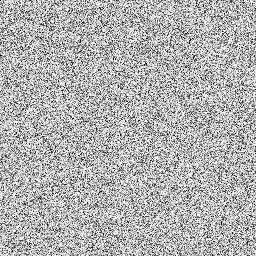
\includegraphics[width=1.25in]{figures/unifnoise1.jpg}
\spc 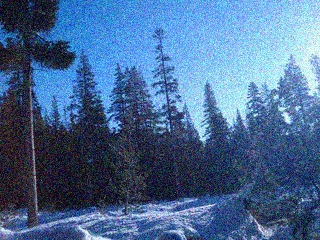
\includegraphics[width=1.65in]{figures/tahoe-gauss.jpg} 
\spc 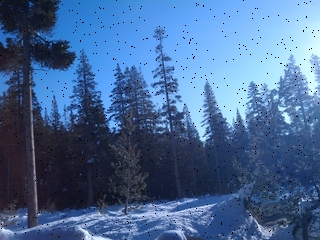
\includegraphics[width=1.65in]{figures/tahoe-pepper.jpg}

\apiend


\apiitem{bool {\ce render_point} (ImageBuf \&dst, int x, int y, \\
  \bigspc\spc\spc array_view<const float> color, \\
  \bigspc\spc\spc ROI roi=ROI.All(), int nthreads=0)}
\index{ImageBufAlgo!render_point} \indexapi{render_point}
Render a point into the destination image,  doing an ``over'' of color (if
it includes an alpha channel). The {\cf color} value should have at least as
many entires as the ROI (which will default to being the entirety of
{\cf dst}). No pixels or channels outside the ROI will be modified.

\smallskip
\noindent Examples:
\begin{code}
    ImageBuf A (ImageSpec (640, 480, 4, TypeDesc::FLOAT));
    float red[4] = { 1, 0, 0, 1 };
    ImageBufAlgo::render_point (A, 50, 100, red);
\end{code}
\apiend


\apiitem{bool {\ce render_line} (ImageBuf \&dst, int x1, int y1, int x2, int y2, \\
  \bigspc\spc\spc array_view<const float> color, \\
  \bigspc\spc\spc bool skip_first_point=false,\\
  \bigspc\spc\spc ROI roi=ROI.All(), int nthreads=0)}
\index{ImageBufAlgo!render_line} \indexapi{render_line}
Render a line from pixel $(x_1,y_1)$ to $(x_2,y_2)$ into {\cf dst}, doing an
``over'' of the color (if it includes an alpha channel) onto the existing
data in {\cf dst}. The {\cf color} must include as many values as {\cf
roi.chend-1}. The ROI can be used to limit the pixel area or channels that
are modified, and default to the entirety of {\cf dst}. If {\cf skip_first_point}
is {\cf true}, the first point {\cf (x1, y1)} will not be drawn (this can
be helpful when drawing poly-lines, to avoid double-rendering of the
vertex positions).

\smallskip
\noindent Examples:
\begin{code}
    ImageBuf A (ImageSpec (640, 480, 4, TypeDesc::FLOAT));
    float red[4] = { 1, 0, 0, 1 };
    ImageBufAlgo::render_line (A, 10, 60, 250, 20, red);
    ImageBufAlgo::render_line (A, 250, 20, 100, 190, red, true);
\end{code}

\spc 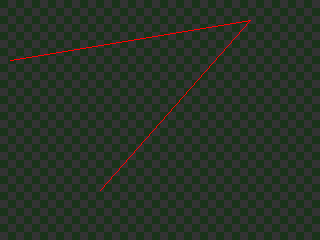
\includegraphics[width=1.65in]{figures/lines.png}  \\
\apiend


\apiitem{bool {\ce render_box} (ImageBuf \&dst, int x1, int y1, int x2, int y2, \\
  \bigspc\spc\spc array_view<const float> color, bool fill=false,\\
  \bigspc\spc\spc roi=ROI.All(), int nthreads=0)}
\index{ImageBufAlgo!render_box} \indexapi{render_box}

Render a filled or unfilled box with corners at pixels $(x_1,y_1)$ and
$(x_2,y_2)$ into {\cf dst}, doing an ``over'' of the color (if it includes
an alpha channel) onto the existing data in {\cf dst}. The {\cf color} must
include as many values as {\cf roi.chend-1}. The ROI can be used to limit
the pixel area or channels that are modified, and default to the entirety of
{\cf dst}. If {\cf fill} is {\cf true}, the box will be completely filled in,
otherwise only its outlien will be drawn.

\smallskip
\noindent Examples:
\begin{code}
    ImageBuf A (ImageSpec (640, 480, 4, TypeDesc::FLOAT));
    float cyan[4] = { 1, 0, 0, 1 };
    ImageBufAlgo::render_box (A, 150, 100, 240, 180, cyan);
    float yellow_transparent[4] = { 0.5, 0.5, 0, 0.5 };
    ImageBufAlgo::render_box (A, 100, 50, 180, 140, yellow_transparent, true);
\end{code}

\spc 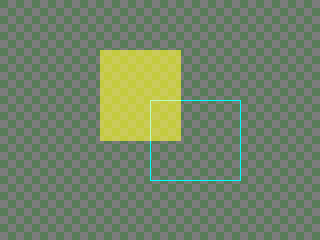
\includegraphics[width=1.65in]{figures/box.png}  \\
\apiend


\apiitem{bool {\ce render_text} (ImageBuf \&dst, int x, int y, string_view text,\\
  \bigspc\spc\spc int fontsize=16, string_view fontname="", \\
  \bigspc\spc\spc  array_view<const float> textcolor = array_view<const float>(),\\
  \bigspc\spc\spc  int shadow = 0, ROI roi = ROI::All(), int nthreads =0)}
\index{ImageBufAlgo!render_text} \indexapi{render_text}


Render a text string (encoded as UTF-8) into image {\cf dst}. If the {\cf dst} image
is not yet initiailzed, it will be initialized to be a black background
exactly large enought to contain the rasterized text.  If {\cf dst} is already
initialized, the text will be rendered into the existing image by
essentially doing an ``over'' of the character into the existing pixel
data.

The font is given by {\cf fontname} (if not a full pathname to a font file, it
will search for a matching font, defaulting to some reasonable system
font if not supplied at all), and with a nominal height of {\cf fontsize} (in
pixels).

The position is given by coordinates ({\cf x,y}), with the default behavior
to align the left edge of the character baseline to ({\cf x,y}). Optionally,
{\cf alignx} and {\cf aligny} can override the alignment behavior, with horizontal
alignment choices of {\cf Left}, {\cf Right}, and {\cf Center}, and vertical alignment
choices of {\cf Baseline}, {\cf Top}, {\cf Bottom}, or {\cf Center}.

The characters will be drawn in opaque white (1.0,1.0,...) in all channels,
unless {\cf textcolor} is supplied (and is expected to point to a float
array of length at least equal to {\cf dst.spec().nchannels}, or defaults
will be chosen for you). If {\cf shadow} is nonzero, a ``drop shadow'' of
that radius will be used to make the text look more clear by dilating the
alpha channel of the composite (makes a black halo around the characters).

\smallskip
\noindent Examples:
\begin{code}
    ImageBufAlgo::render_text (ImgA, 50, 100, "Hello, world");

    float red[] = { 1, 0, 0, 1 };
    ImageBufAlgo::render_text (ImgA, 100, 200, "Go Big Red!",
                               60, "Arial Bold", red);

    float white[] = { 1, 1, 1, 1 };
    ImageBufAlgo::render_text (ImgB, 320, 240, "Centered",
                               60, "Arial Bold", white,
                               TextAlignX::Center, TextAlignY::Center);

\end{code}
\spc 
\includegraphics[width=2.5in]{figures/text.jpg} 
\spc 
\includegraphics[width=2.5in]{figures/textcentered.jpg} \\
\apiend


\apiitem{ROI {\ce text_size} (string_view text, int fontsize=16, \\
\bigspc\bigspc string_view fontname="")}
\index{ImageBufAlgo!text_size} \indexapi{text_size}

\NEW % 1.8
The helper function {\cf text_size()} merely computes the dimensions of the
text, returning it as an {\cf ROI}  relative to the left side of the
baseline of the first character. Only the $x$ and $y$ dimensions of the ROI
will be used. The $x$ dimension runs from left to right, and $y$ runs from
top to bottom (image coordinates). For a failure (such as an invalid
font name), the ROI will return {\cf false} if you call its {\cf defined()}
method.

\begin{code}
    // Render text centered in the image, using text_size to find out¨
    // the size we will need and adjusting the coordinates.
    ImageBuf A (ImageSpec (640, 480, 4, TypeDesc::FLOAT));
    ROI Aroi = A.roi();
    ROI size = ImageBufAlgo::text_size ("Centered", 48, "Courier New");
    if (size.defined()) {
        int x = Aroi.xbegin + Aroi.width()/2  - (size.xbegin + size.width()/2);
        int y = Aroi.ybegin + Aroi.height()/2 - (size.ybegin + size.height()/2);
        ImageBufAlgo::render_text (A, x, y, "Centered", 48, "Courier New");
    }
\end{code}
%\spc 
\includegraphics[width=2.0in]{figures/textcentered.jpg} \\
\apiend





\section{Image transformations and data movement}
\label{sec:iba:transforms}

\apiitem{bool {\ce channels} (ImageBuf \&dst, const ImageBuf \&src, int nchannels, \\
        \bigspc  const int *channelorder,  const float *channelvalues=NULL, \\
        \bigspc  const std::string *newchannelnames=NULL, \\
        \bigspc  bool shuffle_channel_names=false, int nthreads=0)}
\index{ImageBufAlgo!channels} \indexapi{channels} \label{sec:iba:channels}

Generic channel shuffling: copy {\cf src} to {\cf dst}, but with channels in
the order specified by {\cf channelorder[0..nchannels-1]}.  Does not support in-place
operation.  For any channel in which {\cf channelorder[i]} $< 0$, it will
just make {\cf dst} channel {\cf i} be a constant value set to {\cf channelvalues[i]}
(if {\cf channelvalues} is not \NULL) or {\cf 0.0} (if {\cf channelvalues} is \NULL).

If {\cf channelorder} is \NULL, it will be interpreted as
{\cf \{0, 1, ..., nchannels-1\}}, meaning that it's only renaming channels,
not reordering them.

If {\cf newchannelnames} is not \NULL, it points to an array of new channel
names.  Channels for which {\cf newchannelnames[i]} is the empty string (or
all channels, if {\cf newchannelnames == NULL}) will be named as follows:
If {\cf shuffle_channel_names} is {\cf false}, the resulting dst image will have
default channel names in the usual order (\qkw{R}, \qkw{G}, etc.), but if
{\cf shuffle_channel_names} is {\cf true}, the names will be taken from the
corresponding channels of the source image -- be careful with this,
shuffling both channel ordering and their names could result in no
semantic change at all, if you catch the drift.

\smallskip
\noindent Examples:
\begin{code}
    // Copy the first 3 channels of an RGBA, drop the alpha
    ImageBuf RGBA (...);   // assume it's initialized, 4 chans
    ImageBuf RGB;
    ImageBufAlgo::channels (RGB, RGBA, 3, NULL /*default ordering*/);

    // Copy just the alpha channel, making a 1-channel image
    ImageBuf Alpha;
    int alpha_channel[] = { 3 /* alpha channel */ };
    ImageBufAlgo::channels (Alpha, RGBA, 1, &alpha_channel);

    // Swap the R and B channels
    ImageBuf BRGA;
    int channelorder[] = { 2 /*B*/, 1 /*G*/, 0 /*R*/, 3 /*A*/ };
    ImageBufAlgo::channels (BRGA, RGBA, 4, &channelorder);

    // Add an alpha channel with value 1.0 everywhere to an RGB image,
    // keep the other channels with their old ordering, values, and
    // names.
    int channelorder[] = { 0, 1, 2, -1 /*use a float value*/ };
    float channelvalues[] = { 0 /*ignore*/, 0 /*ignore*/, 0 /*ignore*/, 1.0 };
    std::string channelnames[] = { "", "", "", "A" };
    ImageBufAlgo::channels (RGBA, RGB, 4, channelorder,
                            channelvalues, channelnames);
\end{code}
\apiend

\apiitem{bool {\ce channel_append} (ImageBuf \&dst, const ImageBuf \&A, const ImageBuf \&B, \\
        \bigspc  ROI roi=ROI::All(), int nthreads=0)}
\index{ImageBufAlgo!channel_append} \indexapi{channel_append}
Append the channels of {\cf A} and {\cf B} together into {\cf dst} over
the region of interest.  If the region passed is uninitialized (the
default), it will be interpreted as being the union of the pixel windows
of {\cf A} and {\cf B} (and all channels of both images).  If {\cf dst}
is not already initialized, it will be resized to be big enough for the
region.

\smallskip
\noindent Examples:
\begin{code}
    ImageBuf RGBA (...);   // assume initialized, 4 channels
    ImageBuf Z (...);      // assume initialized, 1 channel
    ImageBuf RGBAZ;
    ImageBufAlgo::channel_append (RGBAZ, RGBA, Z);
\end{code}
\apiend


\apiitem{bool {\ce copy} (ImageBuf \&dst, const ImageBuf \&src, \\
        \bigspc TypeDesc convert=TypeDesc::UNKNOWN, ROI roi=ROI::All(), int nthreads=0)}
\index{ImageBufAlgo!copy} \indexapi{copy}
Copy the specified region of pixels of {\cf src} into {\cf dst} at the same
locations, without changing any existing pixels of {\cf dst} outside the
region.  If {\cf dst} is not already initialized, it will be set to the same
size as {\cf roi} (by default all of {\cf src}, optionally with the pixel
type overridden by {\cf convert} (if it is not {\cf UNKNOWN}).

\smallskip
\noindent Examples:
\begin{code}
    // Set B to be A, but converted to float
    ImageBuf A (...);  // Assume initialized
    ImageBuf B;
    ImageBufAlgo::copy (B, A, TypeDesc::FLOAT);
\end{code}
\apiend


\apiitem{bool {\ce crop} (ImageBuf \&dst, const ImageBuf \&src, \\
        \bigspc  ROI roi=ROI::All(), int nthreads=0)}
\index{ImageBufAlgo!crop} \indexapi{crop}
Reset {\cf dst} to be the specified region of {\cf src}.
Pixels from {\cf src} which are outside {\cf roi} will not be copied, and
new black pixels will be added for regions of {\cf roi} which were outside
the data window of {\cf src}.

Note that the {\cf crop} operation does not actually move the pixels on the
image plane or adjust the full/display window; it merely restricts which
pixels are copied from {\cf src} to {\cf dst}.  (Note the difference
compared to {\cf cut()}).

\smallskip
\noindent Examples:
\begin{code}
    // Set B to be the upper left 200x100 region of A
    ImageBuf A (...);  // Assume initialized
    ImageBuf B;
    ImageBufAlgo::crop (B, A, ROI(0,200,0,100));
\end{code}
\apiend


\apiitem{bool {\ce cut} (ImageBuf \&dst, const ImageBuf \&src, \\
        \bigspc  ROI roi=ROI::All(), int nthreads=0)}
\index{ImageBufAlgo!cut} \indexapi{cut}
Reset {\cf dst} to be the specified region of {\cf src}, but repositioned at
the image plane origin and with the full/display window set to exactly cover
the new pixel window.  (Note the difference compared to {\cf crop()}).

\smallskip
\noindent Examples:
\begin{code}
    // Set B to be the 100x100 region of A with origin (50,200).
    ImageBuf A (...);  // Assume initialized
    ImageBuf B;
    ImageBufAlgo::cut (B, A, ROI(50,250,200,300));
    // Note: B has origin at 0,0, NOT at (50,200).
\end{code}
\apiend


\apiitem{bool {\ce paste} (ImageBuf \&dst, int xbegin, int ybegin, int zbegin,
  int chbegin, \\
  \bigspc const ImageBuf \&src, ROI srcroi=ROI::All(), int nthreads=0)}
\index{ImageBufAlgo!paste} \indexapi{paste}
Copy into {\cf dst}, beginning at {\cf (xbegin, ybegin, zbegin)}, the pixels of
{\cf src} described by {\cf srcroi}.  If {\cf srcroi} is {\cf ROI::All()},
the entirety of src will be used.  It will copy into channels 
{\cf [chbegin...]}, as many channels as are described by {\cf srcroi}.

\smallskip
\noindent Examples:
\begin{code}
    // Paste small.exr on top of big.exr at offset (100,100)
    ImageBuf Big ("big.exr");
    ImageBuf Small ("small.exr");
    ImageBufAlgo::paste (Big, 100, 100, 0, 0, Small);
\end{code}
\apiend


\apiitem{bool {\ce rotate90} (ImageBuf \&dst, const ImageBuf \&src, \\
        \bigspc  ROI roi=ROI::All(), int nthreads=0)}
\index{ImageBufAlgo!rotate90} \indexapi{rotate90}
Copy {\cf src} (or a subregion of {\cf src} to the corresponding pixels
of {\cf dst}, but rotated 90 degrees clockwise.

\smallskip
\noindent Examples:
\begin{code}
    ImageBuf A ("grid.jpg");
    ImageBuf B;
    ImageBufAlgo::rotate90 (B, A);
\end{code}
\spc \includegraphics[width=1.25in]{figures/grid-small.jpg}
~ {\Huge $\rightarrow$} ~
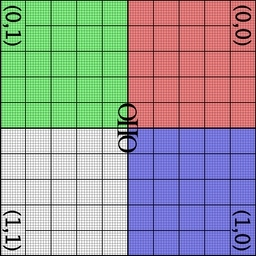
\includegraphics[width=1.25in]{figures/rotate90.jpg} \\
\apiend


\apiitem{bool {\ce rotate180} (ImageBuf \&dst, const ImageBuf \&src, \\
        \bigspc  ROI roi=ROI::All(), int nthreads=0)}
\index{ImageBufAlgo!rotate180} \indexapi{rotate180}
Copy {\cf src} (or a subregion of {\cf src} to the corresponding pixels
of {\cf dst}, but rotated 180 degrees.

\smallskip
\noindent Examples:
\begin{code}
    ImageBuf A ("grid.jpg");
    ImageBuf B;
    ImageBufAlgo::rotate180 (B, A);
\end{code}
\spc \includegraphics[width=1.25in]{figures/grid-small.jpg}
~ {\Huge $\rightarrow$} ~
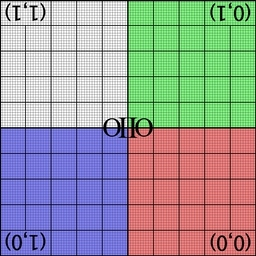
\includegraphics[width=1.25in]{figures/rotate180.jpg} \\
\apiend


\apiitem{bool {\ce rotate270} (ImageBuf \&dst, const ImageBuf \&src, \\
        \bigspc  ROI roi=ROI::All(), int nthreads=0)}
\index{ImageBufAlgo!rotate270} \indexapi{rotate270}
Copy {\cf src} (or a subregion of {\cf src} to the corresponding pixels
of {\cf dst}, but rotated 270 degrees clockwise (or 90 degrees
counter-clockwise).

\smallskip
\noindent Examples:
\begin{code}
    ImageBuf A ("grid.jpg");
    ImageBuf B;
    ImageBufAlgo::rotate270 (B, A);
\end{code}
\spc \includegraphics[width=1.25in]{figures/grid-small.jpg}
~ {\Huge $\rightarrow$} ~
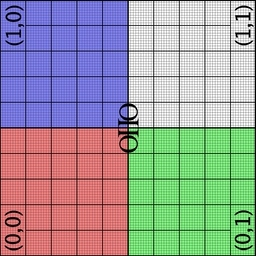
\includegraphics[width=1.25in]{figures/rotate270.jpg} \\
\apiend


\apiitem{bool {\ce flip} (ImageBuf \&dst, const ImageBuf \&src, \\
        \bigspc  ROI roi=ROI::All(), int nthreads=0)}
\index{ImageBufAlgo!flip} \indexapi{flip}
Copy {\cf src} (or a subregion of {\cf src}) to the corresponding pixels
of {\cf dst}, but with the scanlines exchanged vertically.

\smallskip
\noindent Examples:
\begin{code}
    ImageBuf A ("grid.jpg");
    ImageBuf B;
    ImageBufAlgo::flip (B, A);
\end{code}
\spc \includegraphics[width=1.25in]{figures/grid-small.jpg}
~ {\Huge $\rightarrow$} ~
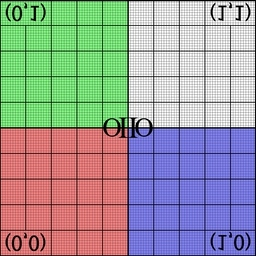
\includegraphics[width=1.25in]{figures/flip.jpg} \\
\apiend


\apiitem{bool {\ce flop} (ImageBuf \&dst, const ImageBuf \&src, \\
        \bigspc  ROI roi=ROI::All(), int nthreads=0)}
\index{ImageBufAlgo!flop} \indexapi{flop}
Copy {\cf src} (or a subregion of {\cf src}) to the corresponding pixels
of {\cf dst}, but with the columns exchanged horizontally.
\smallskip
\noindent Examples:
\begin{code}
    ImageBuf A ("grid.jpg");
    ImageBuf B;
    ImageBufAlgo::flop (B, A);
\end{code}
\spc \includegraphics[width=1.25in]{figures/grid-small.jpg}
~ {\Huge $\rightarrow$} ~
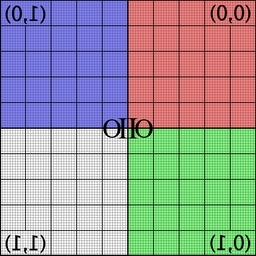
\includegraphics[width=1.25in]{figures/flop.jpg} \\
\apiend


\apiitem{bool {\ce reorient} (ImageBuf \&dst, const ImageBuf \&src, \\
        \bigspc  ROI roi=ROI::All(), int nthreads=0)}
\index{ImageBufAlgo!reorient} \indexapi{reorient}
Copy {\cf src} to {\cf dst}, but with whatever seties of rotations, flips,
or flops are necessary to transform the pixels into the configuration
suggested by the \qkw{Orientation} metadata of the image (and the
\qkw{Orientation} metadata is then set to 1, ordinary orientation).

It is allowed for {\cf src} and {\cf dst} to refer to the same image, in
which case the operation will be done ``in place'' (though not in a way
that is safe for another thread to be accessing the image simultaneously).

\smallskip
\noindent Examples:
\begin{code}
    ImageBuf A ("tahoe.jpg");
    ImageBufAlgo::reorient (A, A);
\end{code}
%\spc \includegraphics[width=1.25in]{figures/grid-small.jpg}
%~ {\Huge $\rightarrow$} ~
%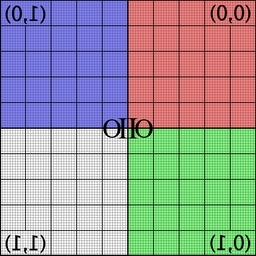
\includegraphics[width=1.25in]{figures/flop.jpg} \\
\apiend


\apiitem{bool {\ce transpose} (ImageBuf \&dst, const ImageBuf \&src, \\
        \bigspc  ROI roi=ROI::All(), int nthreads=0)}
\index{ImageBufAlgo!transpose} \indexapi{transpose}
Copy {\cf src} (or a subregion of {\cf src} to the corresponding 
transposed ($x \leftrightarrow y$) pixels
of {\cf dst}.  In other words, for all $(x,y)$ within the region,
set {\cf dst[y,x] = src[x,y]}.

\smallskip
\noindent Examples:
\begin{code}
    ImageBuf A ("grid.jpg");
    ImageBuf B;
    ImageBufAlgo::transpose (B, A);
\end{code}
\spc \includegraphics[width=1.25in]{figures/grid-small.jpg}
~ {\Huge $\rightarrow$} ~
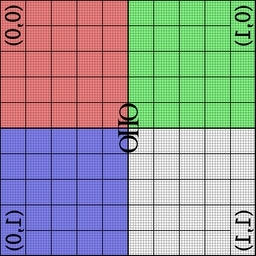
\includegraphics[width=1.25in]{figures/transpose.jpg} \\
\apiend


\apiitem{bool {\ce circular_shift} (ImageBuf \&dst, const ImageBuf \&src, \\
        \bigspc int xshift, int yshift, int zshift=0, \\
        \bigspc  ROI roi=ROI::All(), int nthreads=0)}
\index{ImageBufAlgo!circular_shift} \indexapi{circular_shift}

Copy {\cf src} (or a subregion of {\cf src} to the pixels of {\cf dst},
but circularly shifting by the given amount.  To clarify, the circular
shift of $[0,1,2,3,4,5]$ by $+2$ is $[4,5,0,1,2,3]$.

\smallskip
\noindent Examples:
\begin{code}
    ImageBuf A ("grid.jpg");
    ImageBuf B;
    ImageBufAlgo::circular_shift (B, A, 70, 30);
\end{code}
\spc \includegraphics[width=1.25in]{figures/grid-small.jpg} 
~ {\Huge $\rightarrow$} ~
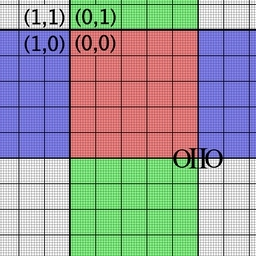
\includegraphics[width=1.25in]{figures/cshift.jpg} \\
\apiend


\apiitem{bool {\ce rotate} (ImageBuf \&dst, const ImageBuf \&src, \\
        \bigspc float angle, \\
        \bigspc string_view filtername="", float filtersize=0, \\
        \bigspc bool recompute_roi = false, \\
        \bigspc ROI roi=ROI::All(), int nthreads=0) \\
bool {\ce rotate} (ImageBuf \&dst, const ImageBuf \&src, \\
        \bigspc float angle, \\
        \bigspc Filter2D *filter, \\
        \bigspc bool recompute_roi = false, \\
        \bigspc ROI roi=ROI::All(), int nthreads=0) \\
bool {\ce rotate} (ImageBuf \&dst, const ImageBuf \&src, \\
        \bigspc float angle, float center_x, float center_y, \\
        \bigspc string_view filtername="", float filtersize=0, \\
        \bigspc bool recompute_roi = false, \\
        \bigspc ROI roi=ROI::All(), int nthreads=0) \\
bool {\ce rotate} (ImageBuf \&dst, const ImageBuf \&src, \\
        \bigspc float angle, float center_x, float center_y, \\
        \bigspc Filter2D *filter, \\
        \bigspc bool recompute_roi = false, \\
        \bigspc ROI roi=ROI::All(), int nthreads=0)}
\index{ImageBufAlgo!rotate} \indexapi{rotate}

Rotate the {\cf src} image by the {\cf angle} (in radians, with positive
angles clockwise). When {\cf center_x} and {\cf center_y} are supplied, they
denote the center of rotation; in their absence, the rotation will be about
the center of the image's display window.

Only the pixels (and channels) of {\cf dst} that are specified by {\cf roi}
will be copied from the rotated {\cf src}; the default {\cf roi} is to alter
all the pixels in {\cf dst}. If {\cf dst} is uninitialized, it will be
resized to be an ImageBuf large enough to hold the rotated image  if
{\cf recompute_roi} is {\cf true}, or will have the same ROI as {\cf src}
if {\cf recompute_roi} is false. It is an
error to pass both an uninitialied {\cf dst} and an undefined {\cf roi}.

The caller may explicitly pass a reconstruction filter, or specify one by
name and size, or if the name is the empty string {\cf rotate()} will choose
a reasonable high-quality default if \NULL is passed.  The filter is used to
weight the {\cf src} pixels falling underneath it for each {\cf dst} pixel;
the filter's size is expressed in pixel units of the {\cf dst} image.

\smallskip
\noindent Examples:
\begin{code}
    ImageBuf Src ("tahoe.exr");
    ImageBuf Dst;
    ImageBufAlgo::rotate (Dst, Src, 45.0);
\end{code}
\spc \includegraphics[width=1.25in]{figures/grid-small.jpg} 
~ {\Huge $\rightarrow$} ~
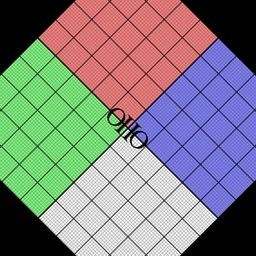
\includegraphics[width=1.25in]{figures/rotate45.jpg} \\
\apiend


\apiitem{bool {\ce warp} (ImageBuf \&dst, const ImageBuf \&src, \\
        \bigspc const Imath::M33f \&M, \\
        \bigspc string_view filtername="", float filtersize=0, \\
        \bigspc bool recompute_roi = false, \\
        \bigspc ImageBuf::WrapMode wrap = ImageBuf::WrapDefault, \\
        \bigspc ROI roi=ROI::All(), int nthreads=0) \\
bool {\ce warp} (ImageBuf \&dst, const ImageBuf \&src, \\
        \bigspc const Imath::M33f \&M, \\
        \bigspc Filter2D *filter, \\
        \bigspc bool recompute_roi = false, \\
        \bigspc ImageBuf::WrapMode wrap = ImageBuf::WrapDefault, \\
        \bigspc ROI roi=ROI::All(), int nthreads=0)}
\index{ImageBufAlgo!warp} \indexapi{warp}

Warp the {\cf src} image using the supplied 3x3 transformation matrix {\cf M}.

Only the pixels (and channels) of {\cf dst} that are specified by {\cf roi}
will be copied from the warped {\cf src}; the default {\cf roi} is to alter
all the pixels in {\cf dst}. If {\cf dst} is uninitialized, it will be
resized to be an \ImageBuf large enough to hold the warped image if
{\cf recompute_roi} is {\cf true}, or will have the same ROI as {\cf src}
if {\cf recompute_roi} is false. It is an
error to pass both an uninitialied {\cf dst} and an undefined {\cf roi}.

The caller may explicitly pass a reconstruction filter, or specify one by
name and size, or if the name is the empty string {\cf resize()} will choose
a reasonable high-quality default if \NULL is passed.  The filter is used to
weight the {\cf src} pixels falling underneath it for each {\cf dst} pixel;
the filter's size is expressed in pixel units of the {\cf dst} image.

\smallskip
\noindent Examples:
\begin{code}
    Imath::M33f M ( 0.7071068, 0.7071068, 0,
                   -0.7071068, 0.7071068, 0,
                   20,        -8.284271,  1);
    ImageBuf Src ("tahoe.exr");
    ImageBuf Dst;
    ImageBufAlgo::warp (dst, src, M, "lanczos3");
\end{code}
\apiend


\apiitem{bool {\ce resize} (ImageBuf \&dst, const ImageBuf \&src, \\
        \bigspc  string_view filtername="", float filtersize=0, \\
        \bigspc  ROI roi=ROI::All(), int nthreads=0) \\
bool {\ce resize} (ImageBuf \&dst, const ImageBuf \&src, \\
        \bigspc Filter2D *filter, \\
        \bigspc  ROI roi=ROI::All(), int nthreads=0)}
\index{ImageBufAlgo!resize} \indexapi{resize}
Set {\cf dst}, over the region of interest, to be a resized version of the
corresponding portion of {\cf src} (mapping such that the ``full'' image
window of each correspond to each other, regardless of resolution).  If
{\cf dst} is not yet initialized, it will be sized according to {\cf roi}.

The caller may explicitly pass a reconstruction filter, or specify one by
name and size, or if the name is the empty string {\cf resize()} will choose
a reasonable high-quality default if \NULL is passed.  The filter is used to
weight the {\cf src} pixels falling underneath it for each {\cf dst} pixel;
the filter's size is expressed in pixel units of the {\cf dst} image.

\smallskip
\noindent Examples:
\begin{code}
    // Resize the image to 640x480, using the default filter
    ImageBuf Src ("tahoe.exr");
    ImageBuf Dst;
    ROI roi (0, 640, 0, 480, 0, 1, /*chans:*/ 0, Src.nchannels());
    ImageBufAlgo::resize (Dst, Src, "", 0, roi);
\end{code}
\apiend


\apiitem{bool {\ce resample} (ImageBuf \&dst, const ImageBuf \&src, \\
        \bigspc bool interpolate = true, \\
        \bigspc ROI roi=ROI::All(), int nthreads=0)}
\index{ImageBufAlgo!resample} \indexapi{resample}
Set {\cf dst}, over the region of interest, to be a resized version of the
corresponding portion of {\cf src} (mapping such that the ``full'' image
window of each correspond to each other, regardless of resolution).  If
{\cf dst} is not yet initialized, it will be sized according to {\cf roi}.

Unlike {\cf ImageBufAlgo::resize()}, {\cf resample()} does not take a filter; it
just samples either with a bilinear interpolation (if {\cf interpolate} is
{\cf true}, the default) or uses the single ``closest'' pixel (if
{\cf interpolate} is {\cf false}).  This makes it a lot faster than a proper
{\cf resize()}, though obviously with lower quality (aliasing when
downsizing, pixel replication when upsizing).

For ``deep'' images, this function returns copies the closest source pixel
needed, rather than attempting to interpolate deep pixels (regardless of the
value of {\cf interpolate}).

\smallskip
\noindent Examples:
\begin{code}
    // Resample quickly to 320x240, using the default filter
    ImageBuf Src ("tahoe.exr");
    ImageBuf Dst;
    ROI roi (0, 320, 0, 240, 0, 1, /*chans:*/ 0, Src.nchannels());
    ImageBufAlgo::resample (Dst, Src, NULL, roi);
\end{code}
\apiend



\section{Image arithmetic}
\label{sec:iba:arith}

\apiitem{bool {\ce add} (ImageBuf \&dst, const ImageBuf \&A, const ImageBuf \&B, \\
        \bigspc  ROI roi=ROI::All(), int nthreads=0) \\
bool {\ce add} (ImageBuf \&dst, const ImageBuf \&A, float B, \\
        \bigspc ROI roi=ROI::All(), int nthreads=0) \\
bool {\ce add} (ImageBuf \&dst, const ImageBuf \&A, const float *B, \\
        \bigspc ROI roi=ROI::All(), int nthreads=0)}
\index{ImageBufAlgo!add} \indexapi{add}

For all pixels and channels within the designated region, set
{\cf dst} to the sum of image {\cf A} and {\cf B}.  {\cf B} is either an image,
a float (added to all channels) or a per-channel float array.
All of the images must have the same number of channels.

\smallskip
\noindent Examples:
\begin{code}
    // Add images A and B, assign to Sum
    ImageBuf A ("a.exr");
    ImageBuf B ("b.exr");
    ImageBuf Sum;
    ImageBufAlgo::add (Sum, A, B);

    // Add 0.2 to channels 0-2 of A
    ImageBuf A ("a.exr"), Sum;
    ROI roi = get_roi (A.spec());
    roi.chbegin = 0;  roi.chend = 3;
    ImageBufAlgo::add (Sum, A, 0.2, roi);
\end{code}
\apiend



\apiitem{bool {\ce sub} (ImageBuf \&dst, const ImageBuf \&A, const ImageBuf \&B, \\
        \bigspc  ROI roi=ROI::All(), int nthreads=0) \\
bool {\ce sub} (ImageBuf \&dst, const ImageBuf \&A, float B, \\
        \bigspc ROI roi=ROI::All(), int nthreads=0) \\
bool {\ce sub} (ImageBuf \&dst, const ImageBuf \&A, const float *B, \\
        \bigspc ROI roi=ROI::All(), int nthreads=0)}
\index{ImageBufAlgo!sub} \indexapi{sub}

For all pixels within the designated region, subtract {\cf B} from {\cf A},
putting the results into {\cf dst}. {\cf B} is either an image, a float
(added to all channels) or a per-channel float array. All of the images must
have the same number of channels.

\smallskip
\noindent Examples:
\begin{code}
    ImageBuf A ("a.exr");
    ImageBuf B ("b.exr");
    ImageBuf Difference;
    ImageBufAlgo::sub (Difference, A, B);
\end{code}
\apiend


\apiitem{bool {\ce absdiff} (ImageBuf \&dst, const ImageBuf \&A, const ImageBuf \&B, \\
        \bigspc  ROI roi=ROI::All(), int nthreads=0) \\
bool {\ce absdiff} (ImageBuf \&dst, const ImageBuf \&A, float B, \\
        \bigspc ROI roi=ROI::All(), int nthreads=0) \\
bool {\ce absdiff} (ImageBuf \&dst, const ImageBuf \&A, const float *B, \\
        \bigspc ROI roi=ROI::All(), int nthreads=0)}
\index{ImageBufAlgo!absdiff} \indexapi{absdiff}

For all pixels within the designated region, compute the absolute value of
the difference between the corresponding pixels of {\cf A} from {\cf B},
putting the results into {\cf dst}. {\cf A} is an \ImageBuf.  {\cf B} may be
an \ImageBuf (with the same number of channels as {\cf A}), or an array of
floats (one per channel, for each channel of {\cf A}), or a single float
(same value for all channels).

\smallskip
\noindent Examples:
\begin{code}
    ImageBuf A ("a.exr");
    ImageBuf B ("b.exr");
    ImageBuf Difference;
    ImageBufAlgo::absdiff (Difference, A, B);
\end{code}
\apiend


\apiitem{bool {\ce abs} (ImageBuf \&dst, const ImageBuf \&A, \\
        \bigspc  ROI roi=ROI::All(), int nthreads=0)}
\index{ImageBufAlgo!abs} \indexapi{abs}

For all pixels within the designated region, compute the absolute value of
the corresponding pixels of {\cf A}, putting the results into {\cf dst}.

\smallskip
\noindent Examples:
\begin{code}
    ImageBuf A ("a.exr");
    ImageBuf Abs;
    ImageBufAlgo::abs (Abs, A);
\end{code}
\apiend



\apiitem{bool {\ce mul} (ImageBuf \&dst, const ImageBuf \&A, const ImageBuf \&B, \\
        \bigspc  ROI roi=ROI::All(), int nthreads=0) \\
bool {\ce mul} (ImageBuf \&dst, const ImageBuf \&A, float B, \\
        \bigspc ROI roi=ROI::All(), int nthreads=0) \\
bool {\ce mul} (ImageBuf \&dst, const ImageBuf \&A, const float *B, \\
        \bigspc ROI roi=ROI::All(), int nthreads=0)}
\index{ImageBufAlgo!mul} \indexapi{mul}

For all pixels within the designated region, multiply the pixel values
of image {\cf A} by {\cf B} (channel by channel), putting the product in
{\cf dst}.  {\cf B} is either an image,
a float (added to all channels) or a per-channel float array.
All of the images must have the same number of channels.

\smallskip
\noindent Examples:
\begin{code}
    ImageBuf A ("a.exr");
    ImageBuf B ("b.exr");
    ImageBuf Product;
    ImageBufAlgo::mul (Product, A, B);

    // Reduce intensity of A's channels 0-2 by 50%
    ROI roi = get_roi (A.spec());
    roi.chbegin = 0;  roi.chend = 3;
    ImageBufAlgo::mul (A, A, 0.5, roi);
\end{code}
\apiend


\apiitem{bool {\ce div} (ImageBuf \&dst, const ImageBuf \&A, const ImageBuf \&B, \\
        \bigspc  ROI roi=ROI::All(), int nthreads=0) \\
bool {\ce div} (ImageBuf \&dst, const ImageBuf \&A, float B, \\
        \bigspc ROI roi=ROI::All(), int nthreads=0) \\
bool {\ce div} (ImageBuf \&dst, const ImageBuf \&A, const float *B, \\
        \bigspc ROI roi=ROI::All(), int nthreads=0)}
\index{ImageBufAlgo!div} \indexapi{div}
For all pixels within the designated region, divide the pixel values
of image {\cf A} by {\cf B} (channel by channel), putting the result in
{\cf dst}.  {\cf B} is either an image,
a float (added to all channels) or a per-channel float array.
All of the images must have the same number of channels.
Division by zero is definied to result in zero.

\smallskip
\noindent Examples:
\begin{code}
    ImageBuf A ("a.exr");
    ImageBuf B ("b.exr");
    ImageBuf Result;
    ImageBufAlgo::div (Result, A, B);

    // Reduce intensity of A's channels 0-2 by 50%
    ROI roi = get_roi (A.spec());
    roi.chbegin = 0;  roi.chend = 3;
    ImageBufAlgo::div (A, A, 2.0f, roi);
\end{code}
\apiend


\apiitem{bool {\ce mad} (ImageBuf \&dst, const ImageBuf \&A, const ImageBuf \&B, \\
        \bigspc  const ImageBuf \&C, ROI roi=ROI::All(), int nthreads=0) \\
bool {\ce mad} (ImageBuf \&dst, const ImageBuf \&A, float B, \\
        \bigspc float C, ROI roi=ROI::All(), int nthreads=0) \\
bool {\ce mad} (ImageBuf \&dst, const ImageBuf \&A, const float *B, \\
        \bigspc const float *C, ROI roi=ROI::All(), int nthreads=0)}
\index{ImageBufAlgo!mad} \indexapi{mad}

For all pixels within the designated region, compute {\cf dst = A * B + C}
(pixel by pixel, channel by channel). {\cf A} must be an image. {\cf B} and
{\cf C} are either both images, both single floats (applied to all
channels), or are both per-channel float arrays. All of the images must have
the same number of channels.

\smallskip
\noindent Examples:
\begin{code}
    ImageBuf A ("a.exr");
    ImageBuf B ("b.exr");
    ImageBuf C ("c.exr");
    ImageBuf Result;
    ImageBufAlgo::mad (Result, A, B, C);

    // Compute the "inverse" A, which is 1.0-A, as A*(-1) + 1
    // Do this in-place, and only for the first 3 channels (leave any
    // alpha channel, if present, as it is).
    ROI roi = get_roi (A.spec());
    roi.chbegin = 0;  roi.chend = 3;
    ImageBufAlgo::mad (A, A, -1.0, 1.0, roi);
\end{code}
\apiend


\apiitem{bool {\ce invert} (ImageBuf \&dst, const ImageBuf \&A, \\
        \bigspc  ROI roi=ROI::All(), int nthreads=0)}
\index{ImageBufAlgo!invert} \indexapi{invert}

For all pixels and channels within the designated region, set {\cf dst}
to be the color inverse of the corresponding pixels of {\cf A}, that is,
1.0 - A.

\smallskip
\noindent Examples:
\begin{code}
    ImageBuf A ("a.exr");
    ImageBuf Inverse;
    ImageBufAlgo::invert (Inverse, A);

    // In this example, we are careful to deal with alpha in an RGBA
    // image. First we copy A to Inverse, and then in-place, we will:
    // un-premultiply the color values by alpha, invert just the color
    // channels, and then re-premultiply the colors by alpha.
    Inverse.copy (A);   // First copy A to inverse
    roi = A.roi();
    roi.chend = 3;      // Restrict roi to only R,G,B
    ImageBufAlgo::unpremult (Inverse, Inverse);
    ImageBufAlgo::invert (Inverse, Inverse, roi);
    ImageBufAlgo::premult (Inverse, Inverse);
\end{code}

%\spc \includegraphics[width=1.5in]{figures/tahoe-small.jpg}
%\raisebox{40pt}{\large $\rightarrow$}
%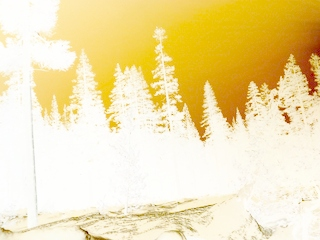
\includegraphics[width=1.5in]{figures/invert.jpg} \\
\apiend


\apiitem{bool {\ce pow} (ImageBuf \&dst, const ImageBuf \&A, float b, \\
        \bigspc ROI roi=ROI::All(), int nthreads=0) \\
bool {\ce pow} (ImageBuf \&dst, const ImageBuf \&A, const float *b, \\
        \bigspc ROI roi=ROI::All(), int nthreads=0)}
\index{ImageBufAlgo!pow} \indexapi{pow}

For all pixels within the designated region, raise the pixel value to the
power {\cf b} (channel by channel), putting the result in
{\cf dst}.  The value {\cf b} is either a single 
float (applied to all channels) or a per-channel float array.

\smallskip
\noindent Examples:
\begin{code}
    // Gamma-correct by 2.2 channels 0-2 of the image
    ROI roi = get_roi (A.spec());
    roi.chbegin = 0;  roi.chend = 3;
    ImageBufAlgo::mul (A, A, 1.0f/2.2f, roi);
\end{code}
\apiend


\apiitem{bool {\ce channel_sum} (ImageBuf \&dst, const ImageBuf \&src, \\
        \bigspc\spc const float *weights=NULL, \\
        \bigspc\spc ROI roi=ROI::All(), int nthreads=0)}
\index{ImageBufAlgo!channel_sum} \indexapi{channel_sum}
Converts a multi-channel image into a 1-channel image via a weighted sum
of channels.  For each pixel of {\cf src} within the designated ROI
(defaulting to all of {\cf src}, if not defined), sum the channels
designated by {\cf roi} and store the result in channel 0 of {\cf dst}.
If {\cf weights} is not \NULL, {\cf weight[i]} will provide a
per-channel weight (rather than defaulting to 1.0 for each channel).

\smallskip
\noindent Examples:
\begin{code}
    // Compute luminance via a weighted sum of R,G,B
    // (assuming Rec709 primaries and a linear scale)
    float luma_weights[3] = { .2126, .7152, .0722 };
    ImageBuf A ("a.exr");
    ImageBuf B;
    ROI roi = A.roi();
    roi.chbegin = 0;  roi.chend = 3;
    ImageBufAlgo::channel_sum (B, A, luma_weights, roi);
\end{code}
\apiend



\apiitem{bool {\ce color_map} (ImageBuf \&dst, const ImageBuf \&src, \\
        \bigspc\spc int srcchannel, int nknots, int channels, \\
        \bigspc\spc array_view<const float> knots, \\
        \bigspc\spc ROI roi=ROI::All(), int nthreads=0) \\
bool {\ce color_map} (ImageBuf \&dst, const ImageBuf \&src, \\
        \bigspc\spc int srcchannel, string_view mapname, \\
        \bigspc\spc ROI roi=ROI::All(), int nthreads=0)}
\index{ImageBufAlgo!color_map} \indexapi{color_map}
\NEW % 1.8

Set pixels of {\cf dst} to colors with values determined by looking up a
color map using values of the {\cf src} image, using either the channel
specified by {\cf srcchannel}, or the luminance of {\cf src}'s RGB if {\cf
srcchannel} is -1. This happens for all pixels within the ROI (which
defaults to all of {\cf src}), and if {\cf dst} is not already initialized,
it will be initialized to the ROI and with color channels equal to {\cf channels}.

In the first variant, the values linearly-interpolated color map are
given by {\cf knots[nknots*channels]}.
An input value of 0.0 corresponds to {\cf knots[0..channels-1]}, an input
value of 1.0 corresponds to {\cf knots[(nknots-1)*channels..knots.size()-1]}.

In the second variant, just the name of a color map is specified. Recognized
map names include: \qkw{blue-red}, \qkw{spectrum}, and \qkw{heat}. In all
cases, the implied {\cf channels} is 3.

\smallskip
\noindent Examples:
\begin{code}
    // Use luminance of a.exr (assuming Rec709 primaries and a linear
    // scale) and map to a color spectrum:
    ImageBuf A ("a.exr");
    ImageBuf B;
    ImageBufAlgo::color_map (B, A, -1, "spectrum");

    float mymap[] = { 0.25, 0.25, 0.25,  0, 0.5, 0,  1, 0, 0 };
    ImageBufAlgo::color_map (B, A, -1 /* use luminance */,
                             3 /* num knots */, 3 /* channels */,
                             mymap);
\end{code}

\noindent \begin{tabular}{lllll}
\includegraphics[width=0.9in]{figures/tahoe-small.jpg} &
\includegraphics[width=0.9in]{figures/colormap-blue-red.jpg} &
\includegraphics[width=0.9in]{figures/colormap-spectrum.jpg} &
\includegraphics[width=0.9in]{figures/colormap-heat.jpg} &
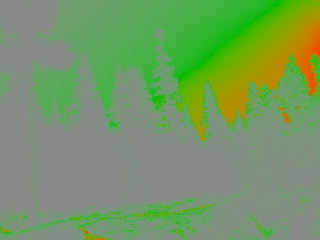
\includegraphics[width=0.9in]{figures/colormap-custom.jpg} \\
original & red-blue & spectrum & heat & custom values \\
\end{tabular}
\apiend



\apiitem{bool {\ce clamp} (ImageBuf \&dst, const ImageBuf \&src, \\
  \bigspc float min = -std::numeric_limits<float>::max(), \\
  \bigspc float max = std::numeric_limits<float>::max(), \\
  \bigspc bool clampalpha01 = false, ROI roi=ROI::All(), int nthreads=0) \\
bool {\ce clamp} (ImageBuf \&dst, const ImageBuf \&src, \\
  \bigspc const float *min = NULL, const float *max = NULL, \\
  \bigspc bool clampalpha01 = false, ROI roi=ROI::All(), int nthreads=0)}
\index{ImageBufAlgo!clamp} \indexapi{clamp}

Copy pixels from {\cf src} to {\cf src} (within the {\cf roi}), clamping
between the {\cf min} and {\cf max} values.  Additionally, if
{\cf clampalpha01} is {\cf true}, then any alpha 
channel is clamped to the 0--1 range.

For the variety of {\cf clamp()} in which the {\cf min} and {\cf max}
values are {\cf float}, the minimum and maximum will be applied to
all color channels (or, at least, the subset of channels specified by
{\cf roi}).

For the variety of {\cf clamp()} in which the {\cf min} and {\cf max}
parameters are pointers, they point to arrays giving per-channel minimum
and maximum clamp values.  If {\cf min} is \NULL, no minimum clamping is
performed, and if {\cf max} is \NULL, no maximum clamping is performed.

\smallskip
\noindent Examples:
\begin{code}
    // Clamp image buffer A in-place to the [0,1] range for all pixels.
    ImageBufAlgo::clamp (A, A, 0.0f, 1.0f);

    // Just clamp alpha to [0,1]
    ImageBufAlgo::clamp (A, A, -std::numeric_limits<float>::max(),
                         std::numeric_limits<float>::max(), true);

    // Clamp R & G to [0,0.5], leave other channels alone
    std::vector<float> min (A.nchannels(), -std::numeric_limits<float>::max());
    std::vector<float> max (A.nchannels(), std::numeric_limits<float>::max());
    min[0] = 0.0f;  max[0] = 0.5f;
    min[1] = 0.0f;  max[1] = 0.5f;
    ImageBufAlgo::clamp (A, A, &min[0], &max[0], false);
\end{code}
\apiend


\apiitem{bool {\ce rangecompress} (ImageBuf \&dst, const ImageBuf \&src, bool useluma = false, \\
        \bigspc\bigspc  ROI roi=ROI::All(), int nthreads=0) \\
bool {\ce rangeexpand} (ImageBuf \&dst, const ImageBuf \&src, bool useluma = false, \\
        \bigspc\bigspc  ROI roi=ROI::All(), int nthreads=0)}
\index{ImageBufAlgo!rangecompress} \indexapi{rangecompress}
\index{ImageBufAlgo!rangeexpand} \indexapi{rangeexpand}

Some image operations (such as resizing with a ``good'' filter that
contains negative lobes) can have objectionable artifacts when applied
to images with very high-contrast regions involving extra bright pixels
(such as highlights in HDR captured or rendered images).  One way to
address this is by compressing the range of pixel values, then
performing the operation (such as a resize), then re-expanding the range
of the result again.  This approach can yield results that are much more
pleasing (even if not exactly mathematically correct).

The {\cf rangecompress} operation does the following: For all pixels and
color channels of {\cf src} within region {\cf roi} (defaulting to all
the defined pixels of {\cf src}), copy the pixels to {\cf dst}
while applying a logarithmic transformation on
their values.  Alpha and z channels are copied but not transformed.

The {\cf rangeexpand} operation is the opposite of {\cf rangecompress}: it
copies while rescaling the logarithmic color channel values back to a linear
response.

If {\cf useluma} is true, the luma of the first three channels (presumed
to be R, G, and B) are used to compute a single scale factor for all
color channels, rather than scaling all channels individually (which
could result in a big color shift when performing {\cf rangecompress}
and {\cf rangeexpand}).

\smallskip
\noindent Examples:
\begin{code}
    // Resize the image to 640x480, using a Lanczos3 filter, which
    // has negative lobes. To prevent those negative lobes from
    // producing ringing or negative pixel values for HDR data,
    // do range compression, then resize, then re-expand the range.

    // 1. Read the original image
    ImageBuf Src ("tahoeHDR.exr");

    // 2. Range compress to a logarithmic scale
    ImageBuf Compressed;
    ImageBufAlgo::rangecompress (Compressed, Src);

    // 3. Now do the resize
    ImageBuf Dst;
    ROI roi (0, 640, 0, 480, 0, 1, /*chans:*/ 0, Compressed.nchannels());
    ImageBufAlgo::resize (Dst, Comrpessed, "lanczos3", 6.0, roi);

    // 4. Expand range to be linear again (operate in-place)
    ImageBufAlgo::rangeexpand (Dst, Dst);
\end{code}
\apiend


\apiitem{bool {\ce over} (ImageBuf \&dst, const ImageBuf \&A, const ImageBuf \&B, \\
        \bigspc  ROI roi=ROI::All(), int nthreads=0)}
\index{ImageBufAlgo!over} \indexapi{over}

For all pixels within the designated region, combine the pixels of
images {\cf A} and {\cf B} using the Porter-Duff ``over'' compositing
operation, putting the result in {\cf dst}.  Image {\cf A} is the
``foreground,'' and {\cf B} is the ``background.''  Images {\cf A} and
{\cf B} must have the same number of channels and must both have an
alpha channel.

\smallskip
\noindent Examples:
\begin{code}
    ImageBuf A ("fg.exr");
    ImageBuf B ("bg.exr");
    ImageBuf Composite;
    ImageBufAlgo::over (Composite, A, B);
\end{code}
\apiend


\apiitem{bool {\ce zover} (ImageBuf \&dst, const ImageBuf \&A, const ImageBuf \&B, \\
        \bigspc  bool z_zeroisinf = false, ROI roi=ROI::All(), int nthreads=0)}
\index{ImageBufAlgo!zover} \indexapi{zover}

For all pixels within the designated region, combine the pixels of
images {\cf A} and {\cf B} using the Porter-Duff ``over'' compositing
operation, putting the result in {\cf dst}.  {\cf A} and {\cf B} must
have the same number of channels and must both alpha and $z$ (depth)
channels. Rather than {\cf A} always being the foreground (as it would
be for the {\cf over()} function, the $z$ channel is used to select
which image is foreground and which is background for each pixel
separately, with a lower $z$ value being the foreground for that pixel.
If {\cf z_zeroisinf} is {\cf true}, then $z=0$ values will be treated
as if they are infinitely far away.

\smallskip
\noindent Examples:
\begin{code}
    ImageBuf A ("a.exr");
    ImageBuf B ("b.exr");
    ImageBuf Composite;
    ImageBufAlgo::zover (Composite, A, B);
\end{code}
\apiend


\section{Image comparison and statistics}
\label{sec:iba:stats}

\apiitem{bool {\ce computePixelStats} (PixelStats \&stats, const ImageBuf \&src, \\
   \bigspc\bigspc  ROI roi=ROI::All(), int nthreads=0)}
\index{ImageBufAlgo!computePixelStats} \indexapi{computePixelStats}
\label{sec:iba:computePixelStats}

Compute statistics about the ROI of the image {\cf src}, storing results
in {\cf stats} (each of the vectors within {\cf stats} will be
automatically resized to the number of channels in the image).  A return
value of {\cf true} indicates success, {\cf false} indicates that it was
not possible to complete the operation.
 The {\cf PixelStats} structure is defined as follows:
\begin{code}
struct PixelStats {
    std::vector<float> min;
    std::vector<float> max;
    std::vector<float> avg;
    std::vector<float> stddev;
    std::vector<imagesize_t> nancount;
    std::vector<imagesize_t> infcount;
    std::vector<imagesize_t> finitecount;
    std::vector<double> sum, sum2;  // for intermediate calculation
};
\end{code}

\smallskip
\noindent Examples:
\begin{code}
    ImageBuf A ("a.exr");
    ImageBufAlgo::PixelStats stats;
    ImageBufAlgo::computePixelStats (stats, A);
    for (int c = 0;  c < A.nchannels();  ++c) {
        std::cout << "Channel " << c << ":\n";
        std::cout << "   min = " << stats.min[c] << "\n";
        std::cout << "   max = " << stats.max[c] << "\n";
        std::cout << "   average = " << stats.avg[c] << "\n";
        std::cout << "   standard deviation  = " << stats.stddev[c] << "\n";
        std::cout << "   # NaN values    = " << stats.nancount[c] << "\n";
        std::cout << "   # Inf values    = " << stats.infcount[c] << "\n";
        std::cout << "   # finite values = " << stats.finitecount[c] << "\n";
    }
\end{code}
\apiend

\apiitem{bool {\ce compare} (const ImageBuf \&A, const ImageBuf \&B, \\
  \bigspc float failthresh, float warnthresh, CompareResults \&result,\\
   \bigspc  ROI roi=ROI::All(), int nthreads=0)}
\index{ImageBufAlgo!compare} \indexapi{compare}

Numerically compare two images.  The difference threshold (for any
individual color channel in any pixel) for a ``failure'' is
{\cf failthresh}, and for a ``warning'' is {\cf warnthresh}.  The 
results are stored in {\cf result}.  If {\cf roi} is defined, pixels
will be compared for the pixel and channel range that is specified.  If
{\cf roi} is not defined, the comparison will be for all channels, on
the union of the defined pixel windows of the two images (for either
image, undefined pixels will be assumed to be black).  The 
{\cf CompareResults} structure is defined as follows:
\begin{code}
struct CompareResults {
    double meanerror, rms_error, PSNR, maxerror;
    int maxx, maxy, maxz, maxc;
    imagesize_t nwarn, nfail;
};
\end{code}

\smallskip
\noindent Examples:
\begin{code}
    ImageBuf A ("a.exr");
    ImageBuf B ("b.exr");
    ImageBufAlgo::CompareResults comp;
    ImageBufAlgo::compare (A, B, 1.0f/255.0f, 0.0f, comp);
    if (comp.nwarn == 0 && comp.nfail == 0) {
        std::cout << "Images match within tolerance\n";
    } else {
        std::cout << "Image differed: " << comp.nfail << " failures, "
                  << comp.nwarn << " warnings.\n";
        std::cout << "Average error was " << comp.meanerror << "\n";
        std::cout << "RMS error was " << comp.rms_error << "\n";
        std::cout << "PSNR was " << comp.PSNR << "\n";
        std::cout << "largest error was " << comp.maxerror 
                  << " on pixel (" << comp.maxx << "," << comp.maxy 
                  << "," << comp.maxz << "), channel " << comp.maxc << "\n";
    }
\end{code}
\apiend


\begin{comment}
 compare_Yee is a bit half-baked. Leave it out of the
  docs for now.  FIXME

\apiitem{int {\ce compare_Yee} (const ImageBuf \&A, const ImageBuf \&B, \\
  \bigspc CompareResults \&result, float luminance, float fov, \\
   \bigspc  ROI roi=ROI::All(), int nthreads=0)}
\index{ImageBufAlgo!compare_Yee} \indexapi{compare_Yee}
\apiend
\end{comment}


\apiitem{bool {\ce isConstantColor} (const ImageBuf \&src, float *color, \\
 \bigspc\bigspc         ROI roi=ROI::All(), int nthreads=0)}
\index{ImageBufAlgo!isConstantColor} \indexapi{isConstantColor}

If all pixels of {\cf src} within the ROI have the same values (for the
subset of channels described by {\cf roi}), return {\cf true} and store
the values in {\cf color[roi.chbegin...roi.chend-1]}.  Otherwise, return
{\cf false}.

\smallskip
\noindent Examples:
\begin{code}
    ImageBuf A ("a.exr");
    std::vector<float> color (A.nchannels());
    if (ImageBufAlgo::isConstantColor (A, &color[0])) {
        std::cout << "The image has the same value in all pixels: ";
        for (int c = 0;  c < A.nchannels();  ++c)
            std::cout << (c ? " " : "") << color[c];
        std::cout << "\n";
    } else {
        std::cout << "The image is not a solid color.\n";
    }
\end{code}
\apiend


\apiitem{bool {\ce isConstantChannel} (const ImageBuf \&src, int channel, float val, \\
 \bigspc\bigspc         ROI roi=ROI::All(), int nthreads=0)}
\index{ImageBufAlgo!isConstantChannel} \indexapi{isConstantChannel}

Returns {\cf true} if all pixels of {\cf src} within the ROI have the
given {\cf channel} value {\cf val}.

\smallskip
\noindent Examples:
\begin{code}
    ImageBuf A ("a.exr");
    int alpha = A.spec().alpha_channel;
    if (alpha < 0)
        std::cout << "The image does not have an alpha channel\n";
    else if (ImageBufAlgo::isConstantChannel (A, alpha, 1.0f))
        std::cout << "The image has alpha = 1.0 everywhere\n";
    else
        std::cout << "The image has alpha < 1 in at least one pixel\n";
\end{code}
\apiend

\apiitem{bool {\ce isMonochrome} (const ImageBuf \&src, 
          ROI roi=ROI::All(), int nthreads=0)}
\index{ImageBufAlgo!isMonochrome} \indexapi{isMonochrome}

Returns {\cf true} if the image is monochrome within the ROI, that is,
for all pixels within the region, do all channels 
{\cf [roi.chbegin, roi.chend)}
have the same value?  If roi is not defined (the default), it will be
understood to be all of the defined pixels and channels of source.

\smallskip
\noindent Examples:
\begin{code}
    ImageBuf A ("a.exr");
    ROI roi = get_roi (A.spec());
    roi.chend = std::min (3, roi.chend);  // only test RGB, not alpha
    if (ImageBufAlgo::isMonochrome (A, roi))
        std::cout << "a.exr is really grayscale\n";
\end{code}
\apiend


\apiitem{bool {\ce color_count} (const ImageBuf \&src, imagesize_t *count,\\
        \bigspc  int ncolors, const float *color, const float *eps=NULL,  \\
        \bigspc  ROI roi=ROI::All(), int nthreads=0)}
\index{ImageBufAlgo!color_count} \indexapi{color_count}

Count how many pixels in the image (within the ROI) match a list of colors.
The colors to match are in:

\begin{code}
  colors[0 ... nchans-1]
  colors[nchans ... 2*nchans-1]
  ...
  colors[(ncolors-1)*nchans ... (ncolors*nchans)-1]
\end{code}

\noindent and so on, a total of {\cf ncolors} consecutively stored
colors of {\cf nchans} channels each ({\cf nchans} is the number of
channels in the image, itself, it is not passed as a parameter).


The values in {\cf eps[0..nchans-1]} are the error tolerances for a
match, for each channel.  Setting {\cf eps[c]} to 
{\cf numeric_limits<float>::max()} will effectively make it ignore the
channel.  Passing {\cf eps == NULL} will be interpreted as a tolerance
of 0.001 for all channels (requires exact matches for 8 bit images, but
allows a wee bit of imprecision for {\cf float} images.

\smallskip
\noindent Examples:
\begin{code}
    ImageBuf A ("a.exr");
    int n = A.nchannels();

    // Try to match two colors: pure red and green
    std::vector<float> colors (2*n, numeric_limits<float>::max());
    colors[0] = 1.0f; colors[1] = 0.0f; colors[2] = 0.0f;
    colors[n+0] = 0.0f; colors[n+1] = 1.0f; colors[n+2] = 0.0f;

    const int ncolors = 2;
    imagesize_t count[ncolors];
    ImageBufAlgo::color_count (A, count, ncolors);
    std::cout << "Number of red pixels   : " << count[0] << "\n";
    std::cout << "Number of green pixels : " << count[1] << "\n";
\end{code}
\apiend


\apiitem{bool {\ce color_range_check} (const ImageBuf \&src, 
   imagesize_t *lowcount, \\ \bigspc imagesize_t *highcount, imagesize_t
  *inrangecount, \\
  \bigspc const float *low, const float *high, \\
        \bigspc  ROI roi=ROI::All(), int nthreads=0)}
\index{ImageBufAlgo!color_range_check} \indexapi{color_range_check}

Count how many pixels in the image (within the ROI) are outside the
value range described by {\cf low[roi.chbegin..roi.chend-1]} and
{\cf high[roi.chbegin..roi.chend-1]} 
as the low and high acceptable values for each color channel.  

The number of pixels containing values that fall below the lower bound
will be stored in {\cf *lowcount}, the number of pixels containing
values that fall above the upper bound will be stored in 
{\cf *highcount}, and the number of pixels for which all channels fell
within the bounds will be stored in {\cf *inrangecount}.  Any of these
may be NULL, which simply means that the counts need not be collected or
stored.

\smallskip
\noindent Examples:
\begin{code}
    ImageBuf A ("a.exr");
    ROI roi = get_roi (A.spec());
    roi.chend = std::min (roi.chend, 4);  // only compare RGBA

    float low[] = {0, 0, 0, 0};
    float high[] = {1, 1, 1, 1};

    imagesize_t lowcount, highcount, inrangecount;
    ImageBufAlgo::color_range_check (A, &lowcount, &highcount, &inrangecount,
                                     low, high, roi);
    std::cout << lowcount << " pixels had components < 0\n";
    std::cout << highcount << " pixels had components > 1\n";
    std::cout << inrangecount << " pixels were fully within [0,1] range\n";
\end{code}
\apiend


\apiitem{ROI {\ce nonzero_region} (const ImageBuf \&src, ROI roi=ROI::All(), int nthreads=0)}
\index{ImageBufAlgo!nonzero_region} \indexapi{nonzero_region}

Find the minimal rectangular region within {\cf roi} (which defaults to
the entire pixel data window of {\cf src}) that consists of nonzero pixel
values.  In other words, gives the region that is a ``shrink-wraps''
of {\cf src} to exclude black border pixels.  Note that if the entire
image was black, the ROI returned will contain no pixels.

For ``deep'' images, this function returns the smallest ROI that contains
all pixels that contain depth samples, and excludes the border pixels
that contain no depth samples at all.

\smallskip
\noindent Examples:
\begin{code}
    ImageBuf A ("a.exr");
    ROI shrunk = ImageBufAlgo::nonzero_region (A);
    if (shrunk.undefined())
        std::cout << "All pixels were empty\n";
    else
        std::cout << "Non-empty region was " << shrunk << "\n";
\end{code}
\apiend


\apiitem{std::string {\ce computePixelHashSHA1} (const ImageBuf \&src, \\
  \bigspc\bigspc string_view extrainfo = "", \\
  \bigspc\bigspc  ROI roi=ROI::All(), int blocksize=0, int nthreads=0)}
\index{ImageBufAlgo!computePixelHashSHA1} \indexapi{computePixelHashSHA1}

Compute the SHA-1 byte hash for all the pixels in the specifed region of
the image.  If {\cf blocksize} $> 0$, the function will compute separate
SHA-1 hashes of each {\cf blocksize} batch of scanlines, then return a
hash of the individual hashes.  This is just as strong a hash, but will
NOT match a single hash of the entire image ({\cf blocksize == 0}).  But
by breaking up the hash into independent blocks, we can parallelize
across multiple threads, given by {\cf nthreads}.
The {\cf extrainfo} provides additional text that will be
incorporated into the hash.

\smallskip
\noindent Examples:
\begin{code}
    ImageBuf A ("a.exr");
    std::string hash;
    hash = ImageBufAlgo::computePixelHashSHA1 (A, "", ROI::All(), 64);
\end{code}
\apiend

\apiitem{bool {\ce histogram} (const ImageBuf \&src, int channel, \\
  \bigspc std::vector<imagesize_t> \&histogram, int bins=256, \\
  \bigspc float min=0, float max=1, imagesize_t *submin=NULL, \\
  \bigspc imagesize_t *supermax=NULL, ROI roi=ROI::All())}
\index{ImageBufAlgo!histogram} \indexapi{histogram}
Computes a histogram of the given {\cf channel} of image {\cf src},
within the ROI,
as follows: The vector {\cf histogram[0..bins-1]} will contain the
count of pixels whose value was in each of the equally-sized range
bins between {\cf min} and {\cf max}; if {\cf submin} is not \NULL,
it specifies storage of the number of pixels whose value was
$<$ {\cf min}; if {\cf supermax} is not \NULL, it specifies storage of
the number of pixels whose value was $>$ {\cf max}.

\smallskip
\noindent Examples:
\begin{code}
    ImageBuf Src ("tahoe.exr");
    const int bins = 4;
    std::vector<imagesize_t> hist (bins, 0);
    imagesize_t submin=0, supermax=0;
    ImageBufAlgo::histogram (Src, 0, hist, bins, 0.0f, 1.0f,
                             &submin, &supermax);
    std::cout << "Channel 0 of the image had:\n";
    float binsize = (max-min)/nbins;
    for (int i = 0;  i < nbins;  ++i)
        hist[i] << " pixels that are >= " << (min+i*binsize) << " and "
                << (i == nbins-1 ? " <= " : " < ")
                << (min+(i+1)*binsize) << "\n";
    std::cout << submin << " pixels < " << min << "\n";
    std::cout << supermax << " pixels > " << max << "\n";
\end{code}
\apiend


\begin{comment}
% I'm not documenting histogram_draw at this point because as I started
% writing this section, I realized I really don't like this function 
% as it is written and would like to rewrite its specification when I
% get the chance.
\apiitem{bool {\ce histogram_draw} (ImageBuf \&dst, 
  \bigspc const std::vector<imagesize_t> \&histogram)}
\index{ImageBufAlgo!histogram_draw} \indexapi{histogram_draw}
\smallskip
\noindent Examples:
\begin{code}
\end{code}
\apiend
\end{comment}


\section{Convolutions}
\label{sec:iba:convolutions}

\apiitem{bool {\ce make_kernel} (ImageBuf \&dst, string_view name, \\
  \bigspc\spc float width, float height, float depth = 1.0f, \\
  \bigspc\spc                         bool normalize = true)}
\index{ImageBufAlgo!make_kernel} \indexapi{make_kernel}
Initialize {\cf dst} to be a 1-channel {\cf float} image of the named kernel.
The size of the {\cf dst} image will be big enough to contain the kernel
given its size ({\cf width} $\times$ {\cf height})
and rounded up to odd resolution so
that the center of the kernel can be at the center of the middle
pixel.  The kernel image will be offset so that its center is at the
{\cf (0,0)} coordinate.  If {\cf normalize} is true, the values will be
normalized so that they sum to $1.0$.

If {\cf depth} $> 1$, a volumetric kernel will be created.  Use with
caution!

Kernel names can be: \qkw{gaussian}, \qkw{sharp-gaussian}, \qkw{box},
\qkw{triangle}, \qkw{mitchell}, \qkw{blackman-harris}, \qkw{b-spline},
\qkw{catmull-rom}, \qkw{lanczos3}, \qkw{cubic}, \qkw{keys}, \qkw{simon},
\qkw{rifman}, \qkw{disk}, \qkw{binomial}, \qkw{laplacian}. Note that
\qkw{catmull-rom} and \qkw{lanczos3} are fixed-size kernels that don't
scale with the width, and are therefore probably less useful in most
cases.

\smallskip
\noindent Examples:
\begin{code}
    ImageBuf K;
    ImageBufAlgo::make_kernel (K, "gaussian", 5.0f, 5.0f);
\end{code}
\apiend

\apiitem{bool {\ce convolve} (ImageBuf \&dst, const ImageBuf \&src, \\
  \bigspc const ImageBuf \&kernel, bool normalize = true, \\
  \bigspc  ROI roi=ROI::All(), int nthreads=0)}
\index{ImageBufAlgo!convolve} \indexapi{convolve}
Replace the given ROI of {\cf dst} with the convolution of {\cf src} and
a kernel.  If {\cf roi} is not defined, it defaults to the full size
of {\cf dst} (or {\cf src}, if {\cf dst} was uninitialized).
If {\cf dst} is uninitialized,
it will be allocated to be the size specified by {\cf roi}.  If 
{\cf normalized} is {\cf true}, the kernel will be normalized for the 
convolution, otherwise the original values will be used.

\smallskip
\noindent Examples:
\begin{code}
    // Blur an image with a 5x5 Gaussian kernel
    ImageBuf Src ("tahoe.exr");
    ImageBuf K;
    ImageBufAlgo::make_kernel (K, "gaussian", 5.0f, 5.0f);
    ImageBuf Blurred;
    ImageBufAlgo::convolve (Blurred, Src, K);
\end{code}

\spc \begin{tabular}{lll}
\includegraphics[width=1.5in]{figures/tahoe-small.jpg} &
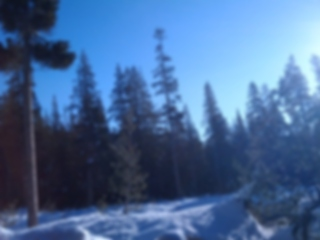
\includegraphics[width=1.5in]{figures/tahoe-blur.jpg} \\
original & blurred \\
\end{tabular}
\apiend

\apiitem{bool {\ce laplacian} (ImageBuf \&dst, const ImageBuf \&src, \\
  \bigspc\spc  ROI roi=ROI::All(), int nthreads=0)}
\index{ImageBufAlgo!laplacian} \indexapi{laplacian}
Replace the given ROI of {\cf dst} with the Laplacian of the corresponding
region of {\cf src}. The Laplacian is the generalized second derivative
of the image,
$$\frac{\partial^2 s}{\partial x^2} + \frac{\partial^2 s}{\partial y^2}$$
which is approximated by convolving the image with a discrete $3 \times 3$
Laplacian kernel,

\[ \left( \begin{array}{ccc}
0 &  1 & 0 \\
1 & -4 & 1 \\
0 &  1 & 0 \end{array} \right)\]

\smallskip
\noindent Example:
\begin{code}
    ImageBuf src ("tahoe.exr");
    ImageBuf dst;
    ImageBufAlgo::laplacian (dst, src);
\end{code}

\spc \begin{tabular}{ll}
\includegraphics[width=1.5in]{figures/tahoe-small.jpg} &
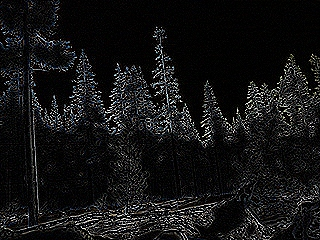
\includegraphics[width=1.5in]{figures/tahoe-laplacian.jpg} \\
original & Laplacian image \\
\end{tabular}

\apiend

\apiitem{bool {\ce fft} (ImageBuf \&dst, const ImageBuf \&src, \\
        \bigspc  ROI roi=ROI::All(), int nthreads=0) \\
        bool {\ce ifft} (ImageBuf \&dst, const ImageBuf \&src, \\
        \bigspc  ROI roi=ROI::All(), int nthreads=0)}
\index{ImageBufAlgo!fft} \indexapi{fft}
\index{ImageBufAlgo!ifft} \indexapi{ifft}

The {\cf fft()} function takes the discrete Fourier transform (DFT) of
the section of {\cf src} denoted by {\cf roi}, storing it in {\cf dst}.
If {\cf roi} is not defined, it will be all of {\cf src}'s pixels.  Only
one channel of {\cf src} may be transformed at a time, so it will be the
first channel described by {\cf roi} (or, again, channel 0 if {\cf roi}
is undefined).  If not already in the correct format, {\cf dst} will be
re-allocated to be a 2-channel {\cf float} buffer of size 
{\cf roi.width()} $\times$ {\cf roi.height}, with channel 0 being the
``real'' part and channel 1 being the the ``imaginary'' part.  The
values returned are actually the unitary DFT, meaning that it is scaled
by $1/\sqrt{\mathrm{npixels}}$.

\smallskip
\noindent Examples:
\begin{code}
    ImageBuf Src ("tahoe.exr");

    // Take the DFT of the first channel of Src
    ImageBuf Freq;
    ImageBufAlgo::fft (Freq, Src);

    // At this point, Freq is a 2-channel float image (real, imag)
    // Convert it back from frequency domain to a spatial image
    ImageBuf Spatial;
    ImageBufAlgo::ifft (Spatial, Freq);
\end{code}
\apiend

\apiitem{bool {\ce complex_to_polar} (ImageBuf \&dst, const ImageBuf \&src, \\
        \bigspc  ROI roi=ROI::All(), int nthreads=0) \\
        bool {\ce polar_to_complex} (ImageBuf \&dst, const ImageBuf \&src, \\
        \bigspc  ROI roi=ROI::All(), int nthreads=0)}
\index{ImageBufAlgo!complex_to_polar} \indexapi{complex_to_polar}
\index{ImageBufAlgo!polar_to_complex} \indexapi{polar_to_complex}

The {\cf polar_to_complex()} function transforms a 2-channel image whose
channels are interpreted as complex values (real and imaginary components)
into the equivalent values expressed in polar form of amplitude and phase
(with phase between $0$ and $2\pi$).

The {\cf complex_to_polar()} function performs the reverse transformation,
converting from  polar values (amplitude and phase) to complex (real and
imaginary).

In either case,  the section of {\cf src} denoted by {\cf roi} is
transformed, storing the result in {\cf dst}. If {\cf roi} is not defined,
it will be all of {\cf src}'s pixels.  Only the first two channels of {\cf
src} will be transformed.

\smallskip
\noindent Examples:
\begin{code}
    // Suppose we have a set of frequency space values expressed as
    // amplitudes and phase...
    ImageBuf Polar ("polar.exr");

    // Convert to complex representation
    ImageBuf Complex;
    ImageBufAlgo::complex_to_polar (Complex, Polar);

    // Now, it's safe to take an IFFT of the complex image.
    // Convert it back from frequency domain to a spatial image.
    ImageBuf Spatial;
    ImageBufAlgo::ifft (Spatial, Complex);
\end{code}
\apiend



\section{Image Enhancement / Restoration}
\label{sec:iba:enhance}

\apiitem{bool {\ce fixNonFinite} (ImageBuf \&dst, const ImageBuf \&src, \\
  \bigspc\spc NonFiniteFixMode mode = NONFINITE_BOX3, \\
  \bigspc\spc int *pixelsFixed = NULL, \\
  \bigspc\spc  ROI roi=ROI::All(), int nthreads=0)}
\index{ImageBufAlgo!fixNonFinite} \indexapi{fixNonFinite}

Copy pixel values from {\cf src} to {\cf dst} (within the pixel and channel
range designated by {\cf roi}), and repair any non-finite ({\cf NaN} or {\cf
Inf}) pixels.  If {\cf pixelsFound} is not \NULL, store in it the number of
pixels that contained non-finite value.

How the non-finite values are repaired is specified by one of the
following modes:

\begin{description} 
\item[\spc] \spc
\item[\rm \kw{NONFINITE_NONE}]   do not alter the pixels (but do count the number
                       of nonfinite pixels in {\cf *pixelsFixed}, if non-\NULL).
\item[\rm \kw{NONFINITE_BLACK}]  change non-finite values to 0.
\item[\rm \kw{NONFINITE_BOX3}]   replace non-finite values by the average of any
                     finite pixels within a 3x3 window.
\item[\rm \kw{NONFINITE_ERROR}]  do not alter non-finite values when copying,
                     but return {\cf false} and set an error if any non-finite
                     values are found.
\end{description}

This works on all pixel data types, though it's just a copy for images with
pixel data types that cannot represent {\cf NaN} or {\cf Inf} values.


\smallskip
\noindent Examples:
\begin{code}
    ImageBuf Src ("tahoe.exr");
    int pixelsFixed = 0;
    ImageBufAlgo::fixNonFinite (Src, Src, ImageBufAlgo::NONFINITE_BOX3,
                                &pixelsFixed);
    std::cout << "Repaired " << pixelsFixed << " non-finite pixels\n";
\end{code}
\apiend


\apiitem{bool {\ce fillholes_pushpull} (ImageBuf \&dst, const ImageBuf \&src, \\
        \bigspc  ROI roi=ROI::All(), int nthreads=0)}
\index{ImageBufAlgo!fillholes_pushpull} \indexapi{fillholes_pushpull}
Copy the specified ROI of {\cf src} to {\cf dst} and fill any 
holes (pixels where alpha $< 1$) with plausible values using a push-pull
technique.  The {\cf src} image must have
an alpha channel.  The dst image will end up with a copy of src, but
will have an alpha of 1.0 everywhere, and any place where the alpha
of src was < 1, dst will have a pixel color that is a plausible
``filling'' of the original alpha hole.

\smallskip
\noindent Examples:
\begin{code}
    ImageBuf Src ("holes.exr");
    ImageBuf Filled;
    ImageBufAlgo::fillholes_pushpull (Filled, Src);
\end{code}
\apiend


\apiitem{bool {\ce median_filter} (ImageBuf \&dst, const ImageBuf \&src, \\
  \bigspc\spc int width = 3, int height = -1, \\
  \bigspc\spc  ROI roi=ROI::All(), int nthreads=0)}
\index{ImageBufAlgo!median_filter} \indexapi{median_filter}

Replace the given ROI of {\cf dst} with a median-filtered version of the
corresponding region of {\cf src}.  The median filter replaces each pixel
with the median value underneath the $\mathit{width} \times \mathit{height}$
window surrounding it. If the height is $< 1$, it will be set to width,
making a square window. The median filter tends to smooth out noise and
small high frequency details that are smaller than the window size, while
preserving the sharpness of long edges.

\smallskip
\noindent Examples:
\begin{code}
    ImageBuf Noisy ("tahoe.exr");
    ImageBuf Clean;
    ImageBufAlgo::median_filter (Clean, Noisy, 3, 3);
\end{code}

\spc \begin{tabular}{lll}
\includegraphics[width=1.5in]{figures/tahoe-small.jpg} &
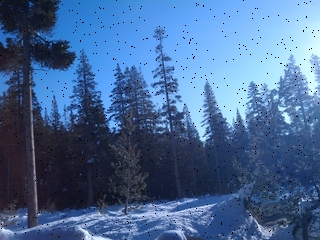
\includegraphics[width=1.5in]{figures/tahoe-pepper.jpg} &
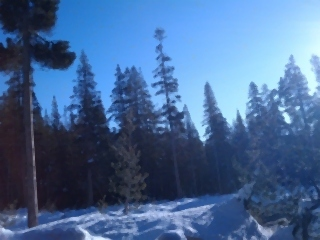
\includegraphics[width=1.5in]{figures/tahoe-pepper-median.jpg} \\
original & with dropouts & median filtered \\
\end{tabular}

\apiend


\apiitem{bool {\ce dilate} (ImageBuf \&dst, const ImageBuf \&src, \\
  \bigspc\spc int width = 3, int height = -1, \\
  \bigspc\spc  ROI roi=ROI::All(), int nthreads=0) \\
bool {\ce erode} (ImageBuf \&dst, const ImageBuf \&src, \\
  \bigspc\spc int width = 3, int height = -1, \\
  \bigspc\spc  ROI roi=ROI::All(), int nthreads=0)}
\index{ImageBufAlgo!dilate} \indexapi{dilate}
\index{ImageBufAlgo!erode} \indexapi{erode}
\index{morphological filtering}

Replace the given ROI of {\cf dst} with the dilated or eroded version of the
corresponding region of {\cf src}.  The dilate operation replaces each pixel
with the maximum value underneath the $\mathit{width} \times \mathit{height}$
window surrounding it, and the erode operation does the same for the minimum
value under the window. If the height is $< 1$, it will be set to width,
making a square window.

Dilation makes bright features wider and more prominent, dark features
thinner, and removes small isolated dark spots. Erosion makes dark features
wider, bright features thinner, and removes small isolated bright spots.

Dilation and erosion are basic morphological filters, and more complex ones
are often constructed from them:
\begin{itemize}
\item
\item ``open'' is erode followed by dilate, and it keeps the overall shape
while removing small bright regions;
\item ``close'' is dilate followed by erode, and it keeps the overall shape
while removing small dark regions;
\item ``morphological gradient'' is dilate minus erode, which gives a
bright perimeter edge;
\item ``tophat'' is the original source minus the ``open'', which isolates
local peaks;
\item ``bottomhat'' is the ``close'' minus the original source, which
isolates dark holes.
\end{itemize}

\smallskip
\noindent Examples:
\begin{code}
    ImageBuf Source ("source.tif");
    ImageBuf Dilate, Erode, Opene, Close, Gradient, Tophat, Bottomhat;
    ImageBufAlgo::dilate (Dilated, Source, 3, 3);
    ImageBufAlgo::erode (Eroded, Source, 3, 3);

    // Morphological "open" is dilate(erode((source))
    ImageBufAlgo::dilate (Opene, Erode, 3, 3);
    // Morphological "close" is erode(dilate(source))
    ImageBufAlgo::erode (Close, Dilate, 3, 3);
    // Morphological "gradient" is dilate minus erode
    ImageBufAlgo::sub (Gradient, Dilate, Erode);
    // Tophat filter is source minus open
    ImageBufAlgo::sub (Tophat, Source, Opene);
    // Bottomhat filter is close minus source
    ImageBufAlgo::sub (Bottomhat, Close, Source);
\end{code}

\spc \begin{tabular}{llll}

\includegraphics[width=0.75in]{figures/morphsource.jpg} &

\includegraphics[width=0.75in]{figures/dilate.jpg} &

\includegraphics[width=0.75in]{figures/erode.jpg} &

\includegraphics[width=0.75in]{figures/morphopen.jpg} \\
original & dilate & erode & open \\

\includegraphics[width=0.75in]{figures/morphclose.jpg} &

\includegraphics[width=0.75in]{figures/morphgradient.jpg} &

\includegraphics[width=0.75in]{figures/tophat.jpg} &
\includegraphics[width=0.75in]{figures/bottomhat.jpg} \\
close & gradient & tophat & bottomhat \\
\end{tabular}

\apiend


\apiitem{bool {\ce unsharp_mask} (ImageBuf \&dst, const ImageBuf \&src, \\
  \bigspc\spc string_view kernel = "gaussian", float width = 3.0f, \\
  \bigspc\spc float contrast = 1.0f, float threshold = 0.0f, \\
  \bigspc\spc  ROI roi=ROI::All(), int nthreads=0)}
\index{ImageBufAlgo!unsharp_mask} \indexapi{unsharp_mask}
\label{sec:iba:unsharpmask}

Replace the given ROI of {\cf dst} with a sharpened version of the
corresponding region of {\cf src} using the ``unsharp mask'' technique.
Unsharp masking basically works by first blurring the image (low
pass filter), subtracting this from the original image, then
adding the residual back to the original to emphasize the edges.
Roughly speaking,

\begin{code}
     dst = src + contrast * thresh(src - blur(src))
\end{code}

The specific blur can be selected by kernel name and width (for example,
\qkw{gaussian} is typical). As a special case, \qkw{median} is also accepted
as the kernel name, in which case a median filter is performed rather than
a blurring convolution (Gaussian and other blurs sometimes over-sharpen edges,
whereas using the median filter will sharpen compact high-frequency details
while not over-sharpening long edges).

The {\cf contrast} is a multiplier on the overall sharpening effect.  The
thresholding step causes all differences less than {\cf threshold} to be
squashed to zero, which can be useful for suppressing sharpening of
low-contrast details (like noise) but allow sharpening of
higher-contrast edges.

\smallskip
\noindent Examples:
\begin{code}
    ImageBuf Blurry ("tahoe.exr");
    ImageBuf Sharp;
    ImageBufAlgo::unsharp_mask (Sharp, Blurry, "gaussian", 5.0f);
\end{code}
\apiend


\section{Color manipulation}
\label{sec:iba:color}

\apiitem{bool {\ce colorconvert} (ImageBuf \&dst, const ImageBuf \&src, \\
  \bigspc\spc string_view from, string_view to, bool unpremult=false, \\
  \bigspc\spc string_view context_key="", string_view context_value="", \\
  \bigspc\spc ColorConfig *colorconfig=NULL, \\
  \bigspc\spc ROI roi=ROI::All(), int nthreads=0) \\
bool {\ce colorconvert} (ImageBuf \&dst, const ImageBuf \&src, \\
  \bigspc\spc const ColorProcessor *processor, bool unpremult=false, \\
  \bigspc\spc  ROI roi=ROI::All(), int nthreads=0)}
\index{ImageBufAlgo!colorconvert} \indexapi{colorconvert}
Copy pixels from {\cf src} to {\cf dst} (within the ROI), while
applying a color transform to the pixel values.
In-place operations ({\cf dst} and {\cf src} being the same image)
are supported.

If {\cf unpremult} is {\cf true}, unpremultiply before color conversion,
then premultiply again after the color conversion.  You may want to use
this flag if your image contains an alpha channel.

The first form of this function specifies the ``from'' and ``to'' color
spaces by name. An optional {\cf ColorConfig} is specified, but {\cf NULL}
is passed, the default OCIO color configuration found by examining the {\cf
\$OCIO} environment variable will be used instead.

The second form is directly passed a {\cf ColorProcessor}, which is is a
special object created by a {\cf ColorConfig} (see {\cf OpenImageIO/color.h}
for details).

The {\cf context_key} and {\cf context_value} may optionally be used
to establish a context (for example, a shot-specific transform).

If OIIO was built with OpenColorIO support enabled, then the transformation
may be between any two spaces supported by the active OCIO configuration, or
may be a ``look'' transformation created by {\cf
ColorConfig::createLookTransform}.  If OIIO was not built with OpenColorIO
support enabled, then the only transformations available are from \qkw{sRGB}
to \qkw{linear} and vice versa.

\smallskip
\noindent Examples:
\begin{code}
    #include <OpenImageIO/imagebufalgo.h>
    #include <OpenImageIO/color.h>
    using namespace OIIO;

    ImageBuf Src ("tahoe.jpg");
    ImageBuf Dst;
    ColorConfig cc;
    ColorProcessor *processor = cc.createColorProcessor ("vd8", "lnf");
    ImageBufAlgo::colorconvert (Dst, Src, processor, true);
    ColorProcessor::deleteColorProcessor (processor);

    // Equivalent, though possibly less efficient if you will be
    // converting many images using the same transformation:
    ImageBuf Src ("tahoe.jpg");
    ImageBuf Dst;
    ImageBufAlgo::colorconvert (Dst, Src, "vd8", "lnf", true);
\end{code}
\apiend

\apiitem{bool {\ce ociolook} (ImageBuf \&dst, const ImageBuf \&src, \\
  \bigspc\spc string_view looks, string_view from, string_view to, \\
  \bigspc\spc bool inverse=false, bool unpremult=false, \\
  \bigspc\spc string_view context_key="", string_view context_value="", \\
  \bigspc\spc ColorConfig *colorconfig=NULL, \\
  \bigspc\spc ROI roi=ROI::All(), int nthreads=0)}
\index{ImageBufAlgo!ociolook} \indexapi{ociolook}
Copy pixels from {\cf src} to {\cf dst} (within the ROI), while
applying an OpenColorIO ``look'' transform to the pixel values.
In-place operations ({\cf dst} and {\cf src} being the same image)
are supported.  The {\cf context_key} and {\cf context_value} may optionally be used
to establish a context (for example, a shot-specific transform).

If {\cf inverse} is {\cf true}, it will reverse the color transformation
and look application.

If {\cf unpremult} is {\cf true}, unpremultiply before color conversion,
then premultiply again after the color conversion.  You may want to use
this flag if your image contains an alpha channel.

An optional {\cf ColorConfig} is specified, but {\cf NULL} is passed, the
default OCIO color configuration found by examining the {\cf \$OCIO}
environment variable will be used instead.

\smallskip
\noindent Examples:
\begin{code}
    ImageBuf Src ("tahoe.jpg");
    ImageBuf Dst;
    ImageBufAlgo::ociolook (Dst, Src, "look", "vd8", "lnf", false, false,
                            "SHOT", "pe0012");
\end{code}
\apiend


\apiitem{bool {\ce ociodisplay} (ImageBuf \&dst, const ImageBuf \&src, \\
  \bigspc\spc string_view display, string_view view, \\
  \bigspc\spc string_view from="", string_view looks="",\\
  \bigspc\spc bool unpremult=false, \\
  \bigspc\spc string_view key="", string_view value="", \\
  \bigspc\spc ColorConfig *colorconfig=NULL, \\
  \bigspc\spc ROI roi=ROI::All(), int nthreads=0)}
\index{ImageBufAlgo!ociodisplay} \indexapi{ociodisplay}
Copy pixels from {\cf src} to {\cf dst} (within the ROI), while
applying an OpenColorIO ``display'' transform to the pixel values.
In-place operations ({\cf dst} and {\cf src} being the same image)
are supported.  If {\cf from} or {\cf looks} are empty, it will not
override the look or source color space (subtly different than
passing \qkw{}, the empty string, which means to use no look or source
space).  The {\cf key} and {\cf value} may optionally be used
to establish a context (for example, a shot-specific transform).

If {\cf inverse} is {\cf true}, it will reverse the color transformation
and look application.

If {\cf unpremult} is {\cf true}, unpremultiply before color conversion,
then premultiply again after the color conversion.  You may want to use
this flag if your image contains an alpha channel.

An optional {\cf ColorConfig} is specified, but {\cf NULL} is passed, the
default OCIO color configuration found by examining the {\cf \$OCIO}
environment variable will be used instead.

\smallskip
\noindent Examples:
\begin{code}
    ImageBuf Src ("tahoe.exr");
    ImageBuf Dst;
    ImageBufAlgo::ociodisplay (Dst, Src, "sRGB", "Film", "lnf", NULL,
                               false, "SHOT", "pe0012");
\end{code}
\apiend


\apiitem{bool {\ce ociofiletransform} (ImageBuf \&dst, const ImageBuf \&src, \\
  \bigspc\spc string_view name, bool inverse=false, bool unpremult=false, \\
  \bigspc\spc ColorConfig *colorconfig=NULL, \\
  \bigspc\spc ROI roi=ROI::All(), int nthreads=0)}
\index{ImageBufAlgo!ociofiletransform} \indexapi{ociofiletransform}
Copy pixels from {\cf src} to {\cf dst} (within the ROI), while applying an
OpenColorIO ``file'' transform to the pixel values. If {\cf inverse} is {\cf
true}, it will reverse the color transformation and look application. In-
place operations ({\cf dst} and {\cf src} being the same image) are
supported.

If {\cf unpremult} is {\cf true}, unpremultiply before color conversion,
then premultiply again after the color conversion.  You may want to use
this flag if your image contains an alpha channel.

An optional {\cf ColorConfig} is specified, but {\cf NULL} is passed, the
default OCIO color configuration found by examining the {\cf \$OCIO}
environment variable will be used instead.

\smallskip
\noindent Examples:
\begin{code}
    ImageBuf Src ("tahoe.jpg");
    ImageBuf Dst;
    ImageBufAlgo::ociofiletransform (Dst, Src, "footransform.csp");
\end{code}
\apiend


\apiitem{bool {\ce unpremult} (ImageBuf \&dst, const ImageBuf \&src,\\
  \bigspc ROI roi=ROI::All(), int nthreads=0)}
\index{ImageBufAlgo!unpremult} \indexapi{unpremult}
Copy pixels from {\cf src} to {\cf dst}, and in the process 
divide all color channels (those not alpha or z) 
by the alpha value, to ``un-premultiply'' them.  This presumes that the
image starts of as ``associated alpha'' a.k.a.\ ``premultipled.''  The
alterations are restricted to the pixels and channels of the supplied
ROI (which defaults to all of {\cf src}).  Pixels in which the alpha
channel is 0 will not be modified (since the operation is undefined in
that case).  This is just a copy if there is no identified alpha channel
(and a no-op if {\cf dst} and {\cf src} are the same image).

\smallskip
\noindent Examples:
\begin{code}
    // Convert in-place from associated alpha to unassociated alpha
    ImageBuf A ("a.exr");
    ImageBufAlgo::unpremult (A, A);
\end{code}
\apiend

\apiitem{bool {\ce premult} (ImageBuf \&dst, const ImageBuf \&src, \\
  \bigspc ROI roi=ROI::All(), int nthreads=0)}
\index{ImageBufAlgo!premult} \indexapi{premult}
Copy pixels from {\cf src} to {\cf dst}, and in the process 
multiply all color channels (those not alpha or z) 
by the alpha value, to ``premultiply'' them.  This presumes that the
image starts of as ``unassociated alpha'' a.k.a.\ ``non-premultipled.''
The alterations are restricted to the pixels and channels of the
supplied ROI (which defaults to all of {\cf src}).  This is just a copy
if there is no identified alpha channel
(and a no-op if {\cf dst} and {\cf src} are the same image).

\smallskip
\noindent Examples:
\begin{code}
    // Convert in-place from unassociated alpha to associated alpha
    ImageBuf A ("a.exr");
    ImageBufAlgo::premult (A, A);
\end{code}
\apiend



\section{Import / export}
\label{sec:iba:importexport}

\apiitem{bool {\ce make_texture} (MakeTextureMode mode, const ImageBuf \&input, \\
\bigspc                             string_view outputfilename,
                             const ImageSpec \&config,\\
\bigspc                             std::ostream *outstream = NULL) \\
bool {\ce make_texture} (MakeTextureMode mode, string_view filename, \\
\bigspc                             string_view outputfilename,
                             const ImageSpec \&config,\\
\bigspc                             std::ostream *outstream = NULL)}
\index{ImageBufAlgo!make_texture} \indexapi{make_texture}

Turn an image file (either an existing \ImageBuf or specified by {\cf
filename}) into a tiled, MIP-mapped, texture file and write to the
file named by ({\cf outputfilename}).  The {\cf mode} describes what type of texture file we
are creating and may be one of the following:

\noindent \begin{tabular}{p{2in}p{3in}}
{\cf MakeTxTexture} & Ordinary 2D texture\\
%MakeTxShadow & \\
{\cf MakeTxEnvLatl} & Latitude-longitude environment map\\
{\cf \small MakeTxEnvLatlFromLightProbe} & Latitude-longitude environment map
       constructed from a ``light probe'' image.\\
\end{tabular}

If the {\cf outstream} pointer is not \NULL, it should point
to a stream (for example, {\cf \&std::out}, or a pointer to a local 
{\cf std::stringstream} to capture output), which is where console output
and error messages will be deposited.

The {\cf config} is an \ImageSpec that contains all the information and
special instructions for making the texture.  Anything set in {\cf config}
(format, tile size, or named metadata) will take precedence over
whatever is specified by the input file itself.  Additionally, named
metadata that starts with \qkw{maketx:} will not be output to the file
itself, but may contain instructions controlling how the texture is
created.  The full list of supported configuration options is:

\noindent Named fields:

\begin{tabular}{ >{\cf}l p{4in}}
   format         & Data format of the texture file (default: UNKNOWN =
                    same format as the input) \\
   tile_width     & \multirow{3}{*}{Preferred tile size (default: 64x64x1)} \\
   tile_height    &       \\
   tile_depth     & \\
\end{tabular}
\medskip

\noindent Metadata in {\cf config.extra_attribs}:

\begin{longtable}{ >{\spc \cf\small}p{1.8in} >{\cf\small}l p{3in}}
   compression & string &   Default: "zip" \\
   fovcot & float &          Default: aspect ratio of the image resolution \\
   planarconfig & string &  Default: "separate" \\
   worldtocamera & matrix &  World-to-camera matrix of the view. \\
   worldtoscreen & matrix &  World-to-screen space matrix of the view. \\
   wrapmodes & string &     Default: "black,black" \\
   maketx:verbose & int &    How much detail should go to outstream (0). \\
   maketx:stats & int &      If nonzero, print stats to outstream (0). \\
   maketx:resize & int &     If nonzero, resize to power of 2. (0) \\
   maketx:nomipmap & int &   If nonzero, only output the top MIP level (0). \\
   maketx:updatemode & int &  If nonzero, write new output only if the
                             output file doesn't already exist, or is
                             older than the input file, or was created with
                             different command-line arguments. (0) \\
   \multicolumn{2}{l}{\spc \cf\small maketx:constant_color_detect} \\  & int &
                          If nonzero, detect images that are entirely
                            one color, and change them to be low
                            resolution (default: 0). \\
   \multicolumn{2}{l}{\spc \cf\small maketx:monochrome_detect} \\ & int &
                          If nonzero, change RGB images which have
                             R==G==B everywhere to single-channel
                             grayscale (default: 0). \\
   maketx:opaque_detect & int &
                          If nonzero, drop the alpha channel if alpha
                             is 1.0 in all pixels (default: 0). \\
   maketx:unpremult & int &  If nonzero, unpremultiply color by alpha before
                             color conversion, then multiply by alpha
                             after color conversion (default: 0). \\
   {\small maketx:incolorspace} & string & \\
   {\small maketx:outcolorspace} & string &
                          These two together will apply a color conversion
                              (with OpenColorIO, if compiled). Default: \qkw{} \\
   {\small maketx:colorconfig} & string &
                          Specifies a custom OpenColorIO color config file.
                              Default: \qkw{} \\
   maketx:checknan & int &   If nonzero, will consider it an error if the
                              input image has any NaN pixels. (0) \\
   maketx:fixnan & string & If set to "black" or "box3", will attempt
                              to repair any NaN pixels found in the
                              input image (default: "none"). \\
   \multicolumn{2}{l}{\spc \cf\small maketx:set_full_to_pixels} \\ & int &
                          If nonzero, doctors the full/display window
                              of the texture to be identical to the
                              pixel/data window and reset the origin
                              to 0,0 (default: 0). \\
   maketx:filtername & string &
                          If set, will specify the name of a high-quality
                             filter to use when resampling for MIPmap
                             levels. Default: \qkw{}, use bilinear resampling. \\
   maketx:highlightcomp & int &
                          If nonzero, performs highlight compensation --
                             range compression and expansion around 
                             the resize, plus clamping negative plxel
                             values to zero. This reduces ringing when
                             using filters with negative lobes. \\
   maketx:nchannels & int &  If nonzero, will specify how many channels
                             the output texture should have, padding with
                             0 values or dropping channels, if it doesn't
                             the number of channels in the input.
                             (default: 0, meaning keep all input channels) \\
   maketx:channelnames & string &
                          If set, overrides the channel names of the
                             output image (comma-separated). \\
   {\small maketx:fileformatname} & string &
                          If set, will specify the output file format.
                              (default: \qkw{}, meaning infer the format from
                              the output filename) \\
   \multicolumn{2}{l}{\spc \cf\small maketx:prman_metadata} \\ & int &
                          If set, output some metadata that PRMan will
                              need for its textures. (0) \\
   {\small maketx:oiio_options} & int &
                          (Deprecated; all are handled by default) \\
   \multicolumn{2}{l}{\spc \cf\small maketx:prman_options} \\ & int &
                          If nonzero, override a whole bunch of settings 
                              as needed to make textures that are
                              compatible with PRMan. (0) \\
   maketx:mipimages & string &
                          Semicolon-separated list of alternate images
                              to be used for individual MIPmap levels,
                              rather than simply downsizing. (default: \qkw{}) \\
   \multicolumn{2}{l}{\spc \cf\small maketx:full_command_line} \\ & string &
                          The command or program used to generate this
                              call, will be embedded in the metadata.
                              (default: \qkw{}) \\
   \multicolumn{2}{l}{\spc \cf\small maketx:ignore_unassoc} \\ & int &
                          If nonzero, will disbelieve any evidence that
                              the input image is unassociated alpha. (0) \\
   \multicolumn{2}{l}{\spc \cf\small maketx:read_local_MB} \\ & int &
                          If nonzero, will read the full input file locally
                              if it is smaller than this threshold. Zero
                              causes the system to make a good guess at
                                a reasonable threshold (e.g. 1 GB). (0) \\
   maketx:forcefloat & int &
                          Forces a conversion through float data for
                              the sake of ImageBuf math. (1) \\
   maketx:hash & int &
                          Compute the sha1 hash of the file in parallel. (1) \\
   \multicolumn{2}{l}{\spc \cf\small maketx:allow_pixel_shift} \\ & int &
                          Allow up to a half pixel shift per mipmap level.
                              The fastest path may result in a slight shift
                              in the image, accumulated for each mip level
                              with an odd resolution. (0) \\
\end{longtable}

\smallskip
\noindent Examples:
\begin{code}
    // This command line:
    //    maketx in.exr --hicomp --filter lanczos3 --opaque-detect \
    //             -o texture.exr
    // is equivalent to:

    ImageBuf Input ("in.exr");
    ImageSpec config;
    config.attribute ("maketx:highlightcomp", 1);
    config.attribute ("maketx:filtername", "lanczos3");
    config.attribute ("maketx:opaquedetect", 1);
    stringstream s;
    bool ok = ImageBufAlgo::make_texture (ImageBufAlgo::MakeTxTexture,
                                          Input, "texture.exr", config, &s);
    if (! ok)
        std::cout << "make_texture error: " << s.str() << "\n";
\end{code}
\apiend


\apiitem{bool {\ce from_IplImage} (ImageBuf \&dst, const IplImage *ipl, \\
        \bigspc\bigspc  TypeDesc convert = TypeDesc::UNKNOWN)}
\index{ImageBufAlgo!from_IplImage} \indexapi{from_IplImage}
\index{OpenCV}\indexapi{IplImage}\index{Intel Image Library}
Convert an {\cf IplImage}, used by OpenCV and Intel's Image Libray, and
set {\cf dst} to be the same image (copying the pixels).  If {\cf convert} is
not set to {\cf UNKNOWN}, try to establish {\cf dst} as holding that
data type and convert the {\cf IplImage} data.  Return {\cf true} if ok,
{\cf false} if it couldn't figure out how to make the conversion from
{\cf IplImage} to an \ImageBuf.  If OpenImageIO was compiled without OpenCV
support, this function will return false without modifying {\cf dst}.

\begin{comment}
\smallskip
\noindent Examples:
\begin{code}
\end{code}
\end{comment}
\apiend


\apiitem{IplImage* {\ce to_IplImage} (const ImageBuf \&src)}
\index{ImageBufAlgo!to_IplImage} \indexapi{to_IplImage}
\index{OpenCV}\indexapi{IplImage}\index{Intel Image Library}
Construct an {\cf IplImage*}, used by OpenCV and Intel's Image Library,
that is equivalent to the \ImageBuf {\cf src}.  If it is not possible, or
if OpenImageIO was compiled without OpenCV support, then return
\NULL.  The ownership of the {\cf IplImage} is fully transferred to the
calling application.

\begin{comment}
\smallskip
\noindent Examples:
\begin{code}
\end{code}
\end{comment}
\apiend


\apiitem{bool {\ce capture_image} (ImageBuf \&dst, int cameranum, \\
        \bigspc\bigspc  TypeDesc convert = TypeDesc::UNKNOWN)}
\index{ImageBufAlgo!capture_image} \indexapi{capture_image}
Capture a still image from a designated camera.  If able to do so,
store the image in {\cf dst} and return {\cf true}.  If there is no such device,
or support for camera capture is not available (such as if OpenCV
support was not enabled at compile time), return {\cf false} and do not
alter {\cf dst}.

\smallskip
\noindent Examples:
\begin{code}
    ImageBuf WebcamImage;
    ImageBufAlgo::capture_image (WebcamImage, 0, TypeDesc::UINT8);
    WebcamImage.save ("webcam.jpg");
\end{code}
\apiend



\section{Deep images}
\label{sec:iba:deep}

A number of {\cf ImageBufAlgo} functions are designed to work with ``deep''
images. These are detailed below. In general, {\cf ImageBufAlgo} functions
not listed in this section should not be expected to work with deep images.

\subsection{Functions specific to deep images}

\apiitem{bool {\ce deepen} (ImageBuf \&dst, const ImageBuf \&src, float zvalue, \\
        \bigspc  ROI roi=ROI::All(), int nthreads=0)}
\index{ImageBufAlgo!deepen} \indexapi{deepen} \index{deep images}
Copy pixels from regular (not ``deep'') image {\cf src} into deep {\cf dst}.

If the {\cf src} image has a \qkw{Z} channel: if the source pixel's {\cf Z}
channel value is not infinite, the corresponding pixel of {\cf dst} will get
a single depth sample that copies the data from the soruce pixel; otherwise,
{\cf dst} will get an empty pixel. In other words, infinitely far pixels
will not turn into deep samples.

If the {\cf src} image lacks a \qkw{Z} channel: if any of the source pixel's
channel values are nonzero, the corresponding pixel of {\cf dst} will get a
single depth sample that copies the data from the source pixel and uses the
{\cf zvalue} parameter for the depth; otherwise, if all source channels in
that pixel are zero, the destination pixel will get no depth samples.

If {\cf src} is already a deep image, it will just copy pixel values from
{\cf src} to {\cf dst}. If {\cf dst} is not already an initialized
\ImageBuf, it will be sized to match {\cf src} (but made deep).

\smallskip
\noindent Examples:
\begin{code}
    ImageBuf Flat ("RGBAZ.exr");
    ImageBuf Deep;
    ImageBufAlgo::deepen (Deep, Flat);
\end{code}
\apiend

\apiitem{bool {\ce flatten} (ImageBuf \&dst, const ImageBuf \&src, \\
        \bigspc  ROI roi=ROI::All(), int nthreads=0)}
\index{ImageBufAlgo!flatten} \indexapi{flatten} \index{deep images}
Copy pixels from \emph{deep} image {\cf src} into non-deep {\cf dst},
compositing the depth samples within each pixel to yield a single ``flat''
value per pixel. If {\cf src} is not deep, it just copies the pixels without
alteration.

\smallskip
\noindent Examples:
\begin{code}
    ImageBuf Deep ("deepalpha.exr");
    ImageBuf Flat;
    ImageBufAlgo::flatten (Flat, Deep);
\end{code}
\apiend

\apiitem{bool {\ce deep_merge} (ImageBuf \&dst, const ImageBuf \&A, const ImageBuf \&B, \\
        \bigspc\spc bool occlusion_cull=true, ROI roi=ROI::All(), int nthreads=0)}
\index{ImageBufAlgo!deep_merge} \indexapi{deep_merge} \index{deep images}
Merge the samples of two \emph{deep} images {\cf A} and {\cf B} into deep
result {\cf dst}. If {\cf occlusion_cull} is {\cf true}, samples beyond
the first opaque sample will be discarded, otherwise they will be kept.

\smallskip
\noindent Examples:
\begin{code}
    ImageBuf DeepA ("hardsurf.exr");
    ImageBuf DeepB ("volume.exr");
    ImageBuf Merged;
    ImageBufAlgo::deep_merge (Merged, DeepA, DeepB);
\end{code}
\apiend

\apiitem{bool {\ce deep_holdout} (ImageBuf \&dst, const ImageBuf \&src, \\
\bigspc\spc  const ImageBuf \&holdout, ROI roi=ROI::All(), int nthreads=0)}
\index{ImageBufAlgo!deep_holdout} \indexapi{deep_holdout} \index{deep images}
\NEW % 1.8
Set the pixels of {\cf dst} to the samples of {\cf src}, but held out by the
samples of the {\cf holdout} image. A ``holdout'' is an image whose alpha
blocks what's behind it as usual, but doesn't contribute any alpha or color
itself.

\smallskip
\noindent Examples:
\begin{code}
    ImageBuf Img ("image.exr");
    ImageBuf Holdout ("holdout.exr");
    ImageBuf Result;
    ImageBufAlgo::deep_holdout (Result, Img, Holdout);
\end{code}
\apiend


\apiitem{bool {\ce deep_cull} (ImageBuf \&dst, const ImageBuf \&src, \\
\bigspc\spc  const ImageBuf \&holdout, ROI roi=ROI::All(), int nthreads=0)}
\index{ImageBufAlgo!deep_cull} \indexapi{deep_cull} \index{deep images}
\NEW % 1.8
Set the pixels of {\cf dst} to the pixels of {\cf src}, but only copying the
samples that are closer than the opaque frontier of image {\cf holdout}.
That is, {\cf holdout} will serve as a depth holdout mask, but no samples
from {\cf holdout} will actually be copied to {\cf dst}.

\smallskip
\noindent Examples:
\begin{code}
    ImageBuf Img ("image.exr");
    ImageBuf Holdout ("holdout.exr");
    ImageBuf Thresholded;
    ImageBufAlgo::deep_cull (Thresholded, Img, Holdout);
\end{code}
\apiend


\subsection{General functions that also work for deep images}

\apiitem{bool {\ce channels} (ImageBuf \&dst, const ImageBuf \&src, int nchannels, \\
        \bigspc  const int *channelorder,  const float *channelvalues=NULL, \\
        \bigspc                 const std::string *newchannelnames=NULL, \\
        \bigspc                 bool shuffle_channel_names=false)}
Reorder, rename, remove, or add channels to a deep image.
See Section~\ref{sec:iba:channels}
\apiend

\apiitem{bool {\ce compare} (const ImageBuf \&A, const ImageBuf \&B, \\
  \bigspc float failthresh, float warnthresh, CompareResults \&result,\\
   \bigspc  ROI roi=ROI::All(), int nthreads=0)}
Numerically compare two images.
\apiend

\apiitem{bool {\ce computePixelStats} (PixelStats \&stats, const ImageBuf \&src, \\
   \bigspc\bigspc  ROI roi=ROI::All(), int nthreads=0)}
Compute per-channel statistics about the image.
See Section~\ref{sec:iba:computePixelStats}
\apiend

\apiitem{bool {\ce crop} (ImageBuf \&dst, const ImageBuf \&src, \\
        \bigspc  ROI roi=ROI::All(), int nthreads=0)}
\index{ImageBufAlgo!crop} \indexapi{crop}
Reset the data region of {\cf dst} to be the specified region of {\cf src}.
\apiend

\apiitem{ROI {\ce nonzero_region} (const ImageBuf \&src, ROI roi=ROI::All(), int nthreads=0)}
\index{ImageBufAlgo!nonzero_region} \indexapi{nonzero_region}
For ``deep'' images, this function returns the smallest ROI that contains
all pixels that contain depth samples, and excludes the border pixels
that contain no depth samples at all.
\apiend

\apiitem{bool {\ce add} (ImageBuf \&dst, const ImageBuf \&A, const float *B, \\
        \bigspc ROI roi=ROI::All(), int nthreads=0) \\
bool {\ce sub} (ImageBuf \&dst, const ImageBuf \&A, const float *B, \\
        \bigspc ROI roi=ROI::All(), int nthreads=0) \\
bool {\ce mul} (ImageBuf \&dst, const ImageBuf \&A, const float *B, \\
        \bigspc ROI roi=ROI::All(), int nthreads=0) \\
bool {\ce div} (ImageBuf \&dst, const ImageBuf \&A, const float *B, \\
        \bigspc ROI roi=ROI::All(), int nthreads=0)}
\index{ImageBufAlgo!add} \indexapi{add}
\index{ImageBufAlgo!sub} \indexapi{sub}
\index{ImageBufAlgo!mul} \indexapi{mul}
\index{ImageBufAlgo!div} \indexapi{div}
Add, subtract, multiply, or divide a deep image {\cf A} by per-channel
values {\cf B[]}, storing the result in deep image {\cf dst}.
\apiend

\apiitem{bool {\ce fixNonFinite} (ImageBuf \&dst, const ImageBuf \&src, \\
  \bigspc\spc NonFiniteFixMode mode = NONFINITE_BOX3, \\
  \bigspc\spc int *pixelsFixed = NULL, \\
  \bigspc\spc  ROI roi=ROI::All(), int nthreads=0)}
\index{ImageBufAlgo!fixNonFinite} \indexapi{fixNonFinite}
Repair nonfinite ({\cf NaN} or {\cf Inf}) values, setting them to 0.0.
\apiend

\apiitem{bool {\ce resample} (ImageBuf \&dst, const ImageBuf \&src, \\
        \bigspc bool interpolate = true, \\
        \bigspc ROI roi=ROI::All(), int nthreads=0)}
\index{ImageBufAlgo!resample} \indexapi{resample}
\NEW % 1.8
Set {\cf dst}, over the region of interest, to be a resized version of the
corresponding portion of {\cf src} (mapping such that the ``full'' image
window of each correspond to each other, regardless of resolution), for each
pixel merely copying the closest deep pixel of the source image (no true
interpolation is done for deep images).
\apiend


\begin{comment}
\apiitem{bool {\ce blah} (ImageBuf \&dst, const ImageBuf \&src, \\
        \bigspc  ROI roi=ROI::All(), int nthreads=0)}
\index{ImageBufAlgo!blah} \indexapi{blah}
Blah.
\smallskip
\noindent Examples:
\begin{code}
\end{code}
\apiend
\end{comment}

\index{ImageBufAlgo|)}
\index{Image Processing|)}

\chapwidthend

\chapter{Python Bindings}
\label{chap:pythonbindings}
\indexapi{Python|()}

\section{Overview}

\OpenImageIO provides Python language bindings for much of its
functionality.

\smallskip

You must ensure that the environment variable {\cf PYTHONPATH} includes
the {\cf python} subdirectory of the \OpenImageIO installation.

\smallskip

A Python program must import the {\cf OpenImageIO} package:
\begin{code}
    import OpenImageIO
\end{code}
\noindent In most of our examples below, we assume that for the sake
of brevity, we will alias the package name as follows:
\begin{code}
    import OpenImageIO as oiio
    from OpenImageIO import ImageInput, ImageOutput
    from OpenImageIO import ImageBuf, ImageSpec, ImageBufAlgo
\end{code}

\section{TypeDesc}
\label{sec:pythontypedesc}

The \TypeDesc class that describes data types of pixels and metadata,
described in detail in Section~\ref{sec:TypeDesc}, is replicated for Python.

\apiitem{BASETYPE}
The {\cf BASETYPE} enum corresponds to the C++ {\cf TypeDesc::BASETYPE} and
contains the following values: \\
{\cf UNKNOWN NONE UINT8 INT8 UINT16 INT16 UINT32 INT32 UINT64 INT64 \\
HALF FLOAT DOUBLE STRING PTR} \\
These names are also exported to the {\cf OpenImageIO} namespace.
\apiend

\apiitem{AGGREGATE}
The {\cf AGGREGATE} enum corresponds to the C++ {\cf TypeDesc::AGGREGATE} and
contains the following values: \\
{\cf SCALAR VEC2 VEC3 VEC4 MATRIX33 MATRIX44} \\
These names are also exported to the {\cf OpenImageIO} namespace.
\apiend

\apiitem{VECSEMANTICS}
The {\cf VECSEMANTICS} enum corresponds to the C++ {\cf TypeDesc::VECSEMANTICS} and
contains the following values: \\
{\cf NOSEMANTICS COLOR POINT VECTOR NORMAL TIMECODE KEYCODE RATIONAL} \\
These names are also exported to the {\cf OpenImageIO} namespace.
\apiend

\apiitem{TypeDesc.{\ce TypeDesc} (typename='unknown')}

Construct a {\cf TypeDesc} object the easy way: from a string description.
If the type name is omitted, it will default to {\cf UNKNOWN}.

\noindent Examples:
\begin{code}
    import OpenImageIO as oiio

    # make a default (UNKNOWN) TypeDesc
    t = TypeDesc()

    # make a TypeDesc describing an unsigned 8 bit int
    t = TypeDesc("uint8")

    # make a TypeDesc describing an array of 14 'float' values
    t = TypeDesc("float[14]")

    # make a TypeDesc describing 3-vector with point semantics
    t = TypeDesc("point")
\end{code}
\apiend

\apiitem{TypeDesc.{\ce TypeDesc} (basetype=oiio.UNKNOWN, aggregate=oiio.SCALAR, \\
\bigspc\spc\spc vecsemantics=NOSEMANTICS, arraylen=0)}

Construct a {\cf TypeDesc} object the hard way: from individual enum tokens
describing the base type, aggregate class, semantic hints, and array length.

\noindent Examples:
\begin{code}
    import OpenImageIO as oiio

    # make a default (UNKNOWN) TypeDesc
    t = TypeDesc()

    # make a TypeDesc describing an unsigned 8 bit int
    t = TypeDesc(oiio.UINT8)

    # make a TypeDesc describing an array of 14 'float' values
    t = TypeDesc(oiio.FLOAT, oiio.SCALAR, oiio.NOSEMANTICS, 14)

    # make a TypeDesc describing a float point
    t = TypeDesc(oiio.FLOAT, oiio.VEC3, oiio.POINT)
\end{code}
\apiend

\apiitem{TypeUnknown TypeString \\
TypeFloat TypeHalf \\
TypeInt TypeUInt TypeInt16 TypeUInt16 \\
TypeColor TypePoint TypeVector TypeNormal TypeFloat4 \\
TypeMatrix TypeMatrix33 \\
TypeTimeCode TypeKeyCode \\
TypeRational \\
}
Pre-constructed \TypeDesc objects for some common types, available in the
outer OpenImageIO scope.

\noindent Example:
\begin{code}
    t = TypeFloat
\end{code}
\apiend

\apiitem{string {\ce str} (TypeDesc)}
Returns a string that describes the \TypeDesc.

\noindent Example:
\begin{code}
    print str(TypeDesc(oiio.UINT16))

    > int16
\end{code}
\apiend

\apiitem{TypeDesc.{\ce basetype} \\
TypeDesc.{\ce aggregate} \\
TypeDesc.{\ce vecsemantics} \\
TypeDesc.{\ce arraylen}}
Access to the raw fields in the \TypeDesc.

\noindent Example:
\begin{code}
    t = TypeDesc(...)
    if t.basetype == oiio.FLOAT :
        print "It's made of floats"
\end{code}
\apiend

\apiitem{int TypeDesc.{\ce size} () \\
int TypeDesc.{\ce basesize} () \\
TypeDesc TypeDesc.{\ce elementtype} () \\
int TypeDesc.{\ce numelements} () \\
int TypeDesc.{\ce elementsize} ()}
The {\cf size()} is the size in bytes, of the type described.  The
{\cf basesize()} is the size in bytes of the {\cf basetype}.

The {\cf elementtype()} is the type of each array element, if it is an
array, or just the full type if it is not an array.  The {\cf elementsize()}
is the size, in bytes, of the {\cf elementtype} (thus, returning the same
value as {\cf size()} if the type is not an array).  The {\cf numelements()}
method returns {\cf arraylen} if it is an array, or {\cf 1} if it is not
an array.

\noindent Example:
\begin{code}
    t = TypeDesc("point[2]")
    print "size =", t.size()
    print "elementtype =", t.elementtype()
    print "elementsize =", t.elementsize()

    > size = 24
    > elementtype = point
    > elementsize = 12
\end{code}
\apiend

\apiitem{bool typedesc {\ce ==} typedesc \\
bool typedesc {\ce !=} typedesc \\
bool TypeDesc.{\ce equivalent} (typedesc) \\}
Test for equality or inequality.  The {\cf equivalent()} method is more
forgiving than {\cf ==}, in that it considers {\cf POINT}, {\cf VECTOR},
and {\cf NORMAL} vector semantics to not constitute a difference from one
another.

\noindent Example:
\begin{code}
    f = TypeDesc("float")
    p = TypeDesc("point")
    v = TypeDesc("vector")
    print "float==point?", (f == p)
    print "vector==point?", (v == p)
    print "float.equivalent(point)?", f.equivalent(p)
    print "vector.equivalent(point)?", v.equivalent(p)

    > float==point? False
    > vector==point? False
    > float.equivalent(point)? False
    > vector.equivalent(point)? True
\end{code}
\apiend


\section{ROI}
\label{sec:pythonroi}

The \ROI class that describes an image extent or region of interest,
explained in deail in Section~\ref{sec:ROI}, is replicated for Python.

\apiitem{{\ce ROI} () \\
{\ce ROI} (xbegin, xend, ybegin, yend) \\
{\ce ROI} (xbegin, xend, ybegin, yend, zbegin, zend) \\
{\ce ROI} (xbegin, xend, ybegin, yend, zbegin, zend, chbegin, chend)}
Construct an \ROI with the given bounds.  The constructor with no 
arguments makes an \ROI that is ``undefined.''

\noindent Example:
\begin{code}
    import OpenImageIO as oiio
    ...
    roi = ROI (0, 640, 0, 480, 0, 1, 0, 4)   # video res RGBA
\end{code}
\apiend

\apiitem{int ROI.{\ce xbegin} \\
int ROI.{\ce xend} \\
int ROI.{\ce ybegin} \\
int ROI.{\ce yend} \\
int ROI.{\ce zbegin} \\
int ROI.{\ce zend} \\
int ROI.{\ce chbegin} \\
int ROI.{\ce chend}}
The basic fields of the \ROI.
\apiend

\apiitem{ROI ROI.{\ce All}}
A pre-constructed undefined \ROI.
\apiend

\apiitem{bool ROI.{\ce defined}}
{\cf True} if the \ROI is defined, {\cf False} if the \ROI is undefined.
\apiend

\apiitem{int ROI.{\ce width} \\
int ROI.{\ce height} \\
int ROI.{\ce depth} \\
int ROI.{\ce nchannels}}
The number of pixels in each dimension, and the number of channels,
as described by the \ROI.
\apiend

\apiitem{int ROI.{\ce npixels}}
The total number of pixels in the region described by the \ROI.
\apiend


\apiitem{ROI {\ce get_roi} (imagespec) \\
ROI {\ce get_roi_full} (imagespec)}
Returns the \ROI corresponding to the pixel data window of the given
\ImageSpec, or the display/full window, respectively.

\noindent Example:
\begin{code}
    spec = ImageSpec(...)
    roi = oiio.get_roi(spec)
\end{code}
\apiend

\apiitem{{\ce set_roi} (imagespec, roi) \\
{\ce set_roi_full} (imagespec, roi)}
Alter the \ImageSpec's resolution and offset to match the passed \ROI.

\noindent Example:
\begin{code}
    # spec is an ImageSpec
    # The following sets the full (display) window to be equal to the
    # pixel data window:
    oiio.set_roi_full (spec, oiio.get_roi(spec))
\end{code}
\apiend


\section{ImageSpec}
\label{sec:pythonimagespec}

The \ImageSpec class that describes an image, explained in deail in
Section~\ref{sec:ImageSpec}, is replicated for Python.

\apiitem{{\ce ImageSpec} ()\\
{\ce ImageSpec} (typedesc) \\
{\ce ImageSpec} (xres, yres, nchannels, typedesc) \\
{\ce ImageSpec} (roi, typedesc)}
Constructors of an \ImageSpec. These correspond directly to the constructors
in the C++ bindings.

\noindent Example:
\begin{code}
    import OpenImageIO as oiio
    ...

    # default ctr
    s = ImageSpec()

    # construct with known pixel type, unknown resolution
    s = ImageSpec(oiio.UINT8)

    # construct with known resolution, channels, pixel data type
    s = ImageSpec(640, 480, 4, "half")

    # construct from an ROI
    s = ImageSpec (ROI(0,640,0,480,0,1,0,3), TypeFloat)
\end{code}
\apiend

\apiitem{ImageSpec.{\ce width}, ImageSpec.{\ce height}, ImageSpec.{\ce depth} \\
ImageSpec.{\ce x}, ImageSpec.{\ce y}, ImageSpec.{\ce z}}
Resolution and offset of the image data ({\cf int} values).

\noindent Example:
\begin{code}
    s = ImageSpec (...)
    print "Data window is ({},{})-({},{})".format (s.x, s.x+s.width-1,
                                                   s.y, s.y+s.height-1)
\end{code}
\apiend

\apiitem{ImageSpec.{\ce full_width}, ImageSpec.{\ce full_height}, ImageSpec.{\ce full_depth} \\
ImageSpec.{\ce full_x}, ImageSpec.{\ce full_y}, ImageSpec.{\ce full_z}}
Resolution and offset of the ``full'' display window ({\cf int} values).
\apiend

\apiitem{ImageSpec.{\ce tile_width}, ImageSpec.{\ce tile_height}, ImageSpec.{\ce tile_depth}}
For tiled images, the resolution of the tiles ({\cf int} values).  Will be
{\cf 0} for  untiled images.
\apiend

\apiitem{typedesc ImageSpec.{\ce format}}
A \TypeDesc describing the pixel data.
\apiend

\apiitem{int ImageSpec.{\ce nchannels}}
An {\cf int} giving the number of color channels in the image.
\apiend

\apiitem{ImageSpec.{\ce channelnames}}
A tuple of strings containing the names of each color channel.
\apiend

\apiitem{ImageSpec.{\ce channelformats}}
If all color channels have the same format, that will be {\cf ImageSpec.format},
and {\cf channelformats} will be {\cf None}.  However, if there are different
formats per channel, they will be stored in {\cf channelformats} as a tuple
of {\cf TypeDesc} objects.

\noindent Example:
\begin{code}
    if spec.channelformats == None:
        print "All color channels are", str(spec.format)
    else:
        print "Channel formats: "
        for t in spec.channelformats:
            print "\t", t
\end{code}
\apiend

\apiitem{ImageSpec.{\ce alpha_channel} \\
ImageSpec.{\ce z_channel}}
The channel index containing the alpha or depth channel, respectively, or
-1 if either one does not exist or cannot be identified.
\apiend

\apiitem{ImageSpec.{\ce deep}}
Hold {\cf True} if the image is a \emph{deep} (multiple samples per pixel)
image, of {\cf False} if it is an ordinary image.
\apiend

\apiitem{ImageSpec.{\ce extra_attribs}}
Direct access to the {\cf extra_attribs} named metadata, appropriate for
iterating over the entire list rather than searching for a particular named
value.

\vspace{-10pt}
\apiitem{len(extra_attribs)}
\vspace{10pt}
Returns the number of extra attributes.
\apiend
\vspace{-24pt}
\apiitem{extra_attribs[i].name}
\vspace{10pt}
The name of the indexed attribute.
\apiend
\vspace{-24pt}
\apiitem{extra_attribs[i].type}
\vspace{10pt}
The type of the indexed attribute, as a \TypeDesc.
\apiend
\vspace{-24pt}
\apiitem{extra_attribs[i].value}
\vspace{10pt}
The value of the indexed attribute.
\apiend

\noindent Example:
\begin{code}
    s = ImageSpec(...)
    ...
    print "extra_attribs size is", len(s.extra_attribs)
    for i in range(len(s.extra_attribs)) :
        print i, s.extra_attribs[i].name, str(s.extra_attribs[i].type), " :"
        print "\t", s.extra_attribs[i].value
    print
\end{code}
\apiend

\apiitem{ImageSpec.{\ce set_format} (typedesc)}
Given a \TypeDesc, sets the {\cf format} field and
clear any per-channel formats in {\cf channelformats}.

\noindent Example:
\begin{code}
    s = ImageSpec ()
    s.set_format (TypeDesc("uint8"))
\end{code}
\apiend

\apiitem{ImageSpec.{\ce default_channel_names} ()}
Sets {\cf channel_names} to the default names given the value of
the {\cf nchannels} field.
\apiend

\apiitem{int ImageSpec.{\ce channelindex} (name)}
Return (as an int) the index of the channel with the given name, or -1
if it does not exist.
\apiend

\apiitem{ImageSpec.{\ce channel_bytes} () \\
ImageSpec.{\ce channel_bytes} (channel, native=False)}
Returns the size of a single channel value, in bytes (as an
{\cf int}).
(Analogous to the C++ member functions, see 
Section~\ref{sec:ImageSpecMemberFuncs} for details.)
\apiend

\apiitem{ImageSpec.{\ce pixel_bytes} () \\
ImageSpec.{\ce pixel_bytes} (native=False) \\
ImageSpec.{\ce pixel_bytes} (chbegin, chend, native=False)}
Returns the size of a pixel, in bytes (as an {\cf int}).
(Analogous to the C++ member functions, see 
Section~\ref{sec:ImageSpecMemberFuncs} for details.)
\apiend

\apiitem{ImageSpec.{\ce scanline_bytes} (native=False) \\
ImageSpec.{\ce tile_bytes} (native=False) \\
ImageSpec.{\ce image_bytes} (native=False)}
Returns the size of a scanline, tile, or the full image, in bytes (as an
{\cf int}). (Analogous to the C++ member functions, see 
Section~\ref{sec:ImageSpecMemberFuncs} for details.)
\apiend

\apiitem{ImageSpec.{\ce tile_pixels} () \\
ImageSpec.{\ce image_pixels} ()}
Returns the number of pixels in a tile or the full image, respectively
(as an {\cf int}). (Analogous to the C++ member functions, see 
Section~\ref{sec:ImageSpecMemberFuncs} for details.)
\apiend

\apiitem{ImageSpec.{\ce erase_attribute} (name, searchtype=TypeUnknown,\\
\bigspc\bigspc\spc casesensitive=False)}
Remove any specified attributes matching the regular expression {\cf name}
from the list of extra_attribs.
\apiend

\apiitem{ImageSpec.{\ce attribute} (name, int) \\
ImageSpec.{\ce attribute} (name, float) \\
ImageSpec.{\ce attribute} (name, string) \\
ImageSpec.{\ce attribute} (name, typedesc, data) \\}
Sets a metadata value in the {\cf extra_attribs}.  If the metadata item
is a single {\cf int}, {\cf float}, or {\cf string}, you can pass it
directly. For other types, you must pass the \TypeDesc and then the
data (for aggregate types or arrays, pass multiple values as a tuple).

\noindent Example:
\begin{code}
    s = ImageSpec (...)
    s.attribute ("foo_str", "blah")
    s.attribute ("foo_int", 14)
    s.attribute ("foo_float", 3.14)
    s.attribute ("foo_vector", TypeDesc.TypeVector, (1, 0, 11))
    s.attribute ("foo_matrix", TypeDesc.TypeMatrix,
                 (1, 0, 0, 0, 0, 2, 0, 0, 0, 0, 1, 0, 1, 2, 3, 1))
\end{code}
\apiend

\apiitem{ImageSpec.{\ce getattribute} (name) \\
ImageSpec.{\ce getattribute} (name, typedesc)}
Retrieves a named metadata value from {\cf extra_attribs}.  The generic
{\cf getattribute()} function returns it regardless of type, or {\cf None}
if the attribute does not exist.  The typed variety will only succeed
if the attribute is actually of that type specified.

\noindent Example:
\begin{code}
    foo = s.getattribute ("foo")   # None if not found
    foo = s.getattribute ("foo", oiio.FLOAT)  # None if not found AND float
\end{code}
\apiend

\apiitem{ImageSpec.{\ce get_int_attribute} (name, defaultval=0) \\
ImageSpec.{\ce get_float_attribute} (name, defaultval=0.0) \\
ImageSpec.{\ce get_string_attribute} (name, defaultval="")}
Retrieves a named metadata value from {\cf extra_attribs}, if it is
found and is of the given type; returns the default value (or a passed
value) if not found.

\noindent Example:
\begin{code}
    # If "foo" is not found, or if it's not an int, return 0
    foo = s.get_int_attribute ("foo")

    # If "foo" is not found, or if it's not a string, return "blah"
    foo = s.get_string_attribute ("foo", "blah")
\end{code}
\apiend

%\apiitem{static ImageSpec.{\ce metadata_val} (paramval, human=False)}
%For a \ParamValue, format its value as a string.
%\apiend

\apiitem{ImageSpec.{\ce serialize} (format="text", verbose="Detailed")}
\NEW % 1.9
Return a string containing the serialization of the \ImageSpec. The {\cf format}
may be either \qkw{text} or \qkw{XML}. The {\cf verbose} may be one of
\qkw{brief}, \qkw{detailed}, or \qkw{detailedhuman}.
\apiend

\apiitem{ImageSpec.{\ce to_xml} ()}
\NEW % 1.9
Equivalent to {\cf serialize ("xml", "detailedhuman")}.
\apiend

\apiitem{ImageSpec.{\ce from_xml} (xml)}
\NEW % 1.9
Initializes the \ImageSpec from the information in the string {\cf xml}
containing an XML-serialized \ImageSpec.
\apiend

\apiitem{ImageSpec.{\ce channel_name} (chan)}
\NEW % 1.9
Returns a string containing the name of the channel with index {\cf chan}.
\apiend

\apiitem{ImageSpec.{\ce channelindex} (name)}
\NEW % 1.9
Return the integer index of the channel with the given {\cf name}, or
-1 if the name is not a name of one of the channels.
\apiend

\apiitem{ImageSpec.{\ce channelformat} (chan)}
\NEW % 1.9
Returns a \TypeDesc of the channel with index {\cf chan}.
\apiend

\apiitem{ImageSpec.{\ce get_channelformats} ()}
\NEW % 1.9
Returns a tuple containing all the channel formats.
\apiend

\apiitem{ImageSpec.{\ce valid_tile_range} (xbegin, xend, ybegin, yend, zbegin, zend)}
\NEW % 1.9
Returns {\cf True} if the given tile range exactly covers a set of tiles, or
{\cf False} if it isn't (or if the image is not tiled).
\apiend


\newpage
\subsection*{Example: Header info}

Here is an illustrative example of the use of \ImageSpec, a working Python
function that opens a file and prints all the relevant header
information:

\begin{tinycode}
#!/usr/bin/env python 
import OpenImageIO as oiio

# Print the contents of an ImageSpec
def print_imagespec (spec, subimage=0, mip=0) :
    if spec.depth <= 1 :
        print ("  resolution %dx%d%+d%+d" % (spec.width, spec.height, spec.x, spec.y))
    else :
        print ("  resolution %dx%d%x%d+d%+d%+d" % 
               (spec.width, spec.height, spec.depth, spec.x, spec.y, spec.z))
    if (spec.width != spec.full_width or spec.height != spec.full_height
        or spec.depth != spec.full_depth) :
        if spec.full_depth <= 1 :
            print ("  full res   %dx%d%+d%+d" % 
                   (spec.full_width, spec.full_height, spec.full_x, spec.full_y))
        else :
            print ("  full res   %dx%d%x%d+d%+d%+d" % 
                   (spec.full_width, spec.full_height, spec.full_depth,
                    spec.full_x, spec.full_y, spec.full_z))
    if spec.tile_width :
        print ("  tile size  %dx%dx%d" % 
               (spec.tile_width, spec.tile_height, spec.tile_depth))
    else :
        print "  untiled"
    if mip >= 1 :
        return
    print "  " + str(spec.nchannels), "channels:", spec.channelnames
    print "  format = ", str(spec.format)
    if len(spec.channelformats) > 0 :
        print "  channelformats = ", spec.channelformats
    print "  alpha channel = ", spec.alpha_channel
    print "  z channel = ", spec.z_channel
    print "  deep = ", spec.deep
    for i in spec.extra_attribs) :
        if type(i.value) == str :
            print " ", i.name, "= \"" + i.value + "\""
        else :
            print " ", i.name, "=", i.value


def poor_mans_iinfo (filename) :
    input = ImageInput.open (filename)
    if not input :
        print 'Could not open "' + filename + '"'
        print "\tError: ", oiio.geterror()
        return
    print 'Opened "' + filename + '" as a ' + input.format_name()
    sub = 0
    mip = 0
    while True :
        if sub > 0 or mip > 0 :
            print "Subimage", sub, "MIP level", mip, ":"
        print_imagespec (input.spec(), mip=mip)
        mip = mip + 1
        if input.seek_subimage (sub, mip) :
            continue    # proceed to next MIP level
        else :
            sub = sub + 1
            mip = 0
            if input.seek_subimage (sub, mip) :
                continue    # proceed to next subimage
        break  # no more MIP levels or subimages
    input.close ()
\end{tinycode}


\section{DeepData}
\label{sec:pythondeepdata}

The \DeepData class describing ``deep'' image data (multiple depth
sample per pixel), which is explained in deail in
Section~\ref{sec:imageinput:deepdata}, is replicated for Python.

\apiitem{{\ce DeepData} ()}
Constructs a \DeepData object. It needs to have its {\cf init()} and
{\cf alloc()} methods called before it can hold any meaningful data.
\apiend

\apiitem{DeepData.{\ce init} (npixels, nchannels, channeltypes, channelnames)}
Initializes this \DeepData to hold {\cf npixels} total pixels, with
{\cf nchannels} color channels. The data types of the channels are
described by {\cf channeltypes}, a tuple of \TypeDesc values (one per
channel), and the names are provided in a tuple of {\cf string}s
{\cf channelnames}. After calling {\cf init}, you still need to set the number of
samples for each pixel (using {\cf set_nsamples}) and then call {\cf alloc()}
to actually allocate the sample memory.
\apiend

\apiitem{bool {\ce DeepData}.initialized ()}
Returns {\cf True} if the \DeepData is initialized at all.
\apiend

\apiitem{bool {\ce DeepData}.allocated ()}
Returns {\cf True} if the \DeepData has already had pixel memory allocated.
\apiend

\apiitem{DeepData.{\ce pixels}}
This {\cf int} field constains the total number of pixels in this
collection of deep data.
\apiend

\apiitem{DeepData.{\ce channels}}
This {\cf int} field constains the number of channels.
\apiend

\apiitem{int DeepData.{\ce A_channel} \\
int DeepData.{\ce AR_channel} \\
int DeepData.{\ce AG_channel} \\
int DeepData.{\ce AB_channel} \\
int DeepData.{\ce Z_channel} \\
int DeepData.{\ce Zback_channel}}
The channel index of certain named channels, or -1 if they don't exist. For
{\cf AR_channel}, {\cf AG_channel}, {\cf AB_channel}, if they don't exist,
they will contain the value of {\cf A_channel}, and {\cf Zback_channel} will
contain the value of {\cf Z_channel} if there is no actual {\cf Zback}.
\apiend

\apiitem{string DeepData.{\ce channelname} (c)}
Retrieve the name of channel {\cf c}.
\apiend

\apiitem{TypeDesc DeepData.{\ce channeltype} (c)}
Retrieve the data type of channel {\cf c}.
\apiend

\apiitem{int DeepData.{\ce channelsize} (c)}
Retrieve the size (in bytes) of one datum of channel {\cf c}.
\apiend

\apiitem{int DeepData.{\ce samplesize} ()}
Retrieve the packed size (in bytes) of all channels of one sample.
\apiend


\apiitem{DeepData.{\ce set_samples} (pixel, nsamples) \\
int DeepData.{\ce samples} (pixel)}
Set or get the number of samples for a given pixel (specified by integer
index).
\apiend

\apiitem{DeepData.{\ce insert_samples} (pixel, samplepos, n) \\
int DeepData.{\ce erase_samples} (pixel, samplepos, n)}
Insert or erase \emph{n} samples starting at the given position of an
indexed pixel.
\apiend

\apiitem{DeepData.{\ce set_deep_value} (pixel, channel, sample, value) \\
DeepData.{\ce set_deep_value_uint} (pixel, channel, sample, value)}
Set specific float or unsigned int value of a given pixel, channel, and
sample index.
\apiend

\apiitem{DeepData.{\ce deep_value} (pixel, channel, sample, value) \\
int DeepData.{\ce deep_value_uint} (pixel, channel, sample)}
Retrieve the specific value of a given pixel,
channel, and sample index (for float or uint channels, respectively).
\apiend

\apiitem{DeepData.{\ce copy_deep_sample} (pixel, sample, src, srcpixel, srcsample)}
Copy a deep sample from \DeepData {\cf src} into this \DeepData.
\apiend

\apiitem{DeepData.{\ce copy_deep_pixel} (pixel, src, srcpixel)}
Copy a deep pixel from \DeepData {\cf src} into this \DeepData.
\apiend

\apiitem{bool DeepData.{\ce split} (pixel, depth)}
Split any samples of the pixel that cross {\cf depth}. Return {\cf True} if
any splits occurred, {\cf False} if the pixel was unmodified.
\apiend

\apiitem{DeepData.{\ce sort} (pixel)}
Sort the samples of the pixel by their Z depth.
\apiend

\apiitem{DeepData.{\ce merge_overlaps} (pixel)}
Merge any adjacent samples in the pixel that exactly overlap in $z$
range. This is only useful if the pixel has previously been split at
all sample starts and ends, and sorted by depth.
\apiend

\apiitem{DeepData.{\ce merge_deep_pixels} (pixel, src, srcpixel)}
Merge the samples of {\cf src}'s pixel into this \DeepData's pixel.
\apiend

\apiitem{DeepData.{\ce occlusion_cull} (pixel)}
Eliminate any samples beyond an opaque sample.
\apiend

\apiitem{float DeepData.{\ce opaque_z} (pixel)}
For the given pixel index. return the $z$ value at which the pixel reaches
full opacity.
\apiend



\section{ImageInput}
\label{sec:pythonimageinput}

See Chapter~\ref{chap:imageinput} for detailed explanations of the
C++ \ImageInput class APIs. The Python APIs are very similar. The biggest
difference is that in C++, the various {\cf read_*} functions write the
pixel values into an already-allocated array that belongs to the caller,
whereas the Python versions allocate and return an array holding the pixel
values (or {\cf None} if the read failed).


\apiitem{ImageInput.{\ce open} (filename) \\
ImageInput.{\ce open} (filename, config_imagespec)}
Creates an \ImageInput object and opens the named file.  Returns the
open \ImageInput upon success, or {\cf None} if it failed to open the
file (after which, {\cf OpenImageIO.geterror()} will contain an error
message).  In the second form, the optional \ImageSpec argument 
{\cf config} contains attributes that may set certain options when opening
the file.

\noindent Example:
\begin{code}
    input = ImageInput.open ("tahoe.jpg")
    if input == None :
        print "Error:", oiio.geterror()
        return
\end{code}
\apiend

\apiitem{bool ImageInput.{\ce close} ()}
Closes an open image file, returning {\cf True} if successful, {\cf False}
otherwise.

\noindent Example:
\begin{code}
    input = ImageInput.open (filename)
    ...
    input.close ()
\end{code}
\apiend


\apiitem{str ImageInput.{\ce format_name} ()}
Returns the format name of the open file.

\noindent Example:
\begin{code}
    input = ImageInput.open (filename)
    if input :
        print filename, "was a", input.format_name(), "file."
        input.close ()
  
\end{code}
\apiend

\apiitem{ImageSpec ImageInput.{\ce spec} ()}
Returns the \ImageSpec corresponding to the currently open subimage and
MIP level of the file.

\noindent Example:
\begin{code}
    input = ImageInput.open (filename)
    spec = input.spec()
    print "resolution ", spec.width, "x", spec.height
\end{code}
\apiend

\apiitem{int ImageInput.{\ce current_subimage} () \\
int ImageInput.{\ce current_miplevel} ()}
Returns the current subimage and/or MIP level of the file.
\apiend

\apiitem{bool ImageInput.{\ce seek_subimage} (subimage, miplevel)}
Repositions the file pointer to the given subimage and MIP level within the
file (starting with {\cf 0}).  This function returns {\cf True} upon success,
{\cf False} upon failure (which may include the file not having the
specified subimage or MIP level).

\noindent Example:
\begin{code}
    input = ImageInput.open (filename)
    mip = 0
    while True :
        ok = input.seek_subimage (0, mip)
        if not ok :
            break
        spec = input.spec()
        print "MIP level", mip, "is", spec.width, "x", spec.height
\end{code}
\apiend

\apiitem{ImageInput.{\ce read_image} (type="float") \\
ImageInput.{\ce read_image} (chbegin, chend, type="float")}

Read the entire image and return the pixels as a NumPy array of values of
the given {\cf type} (described by a \TypeDesc or a string, float by
default). If the {\cf type} is {\cf TypeUnknown}, the pixels will be
returned in the native format of the file. If an error occurs, {\cf None}
will be returned.

For a normal (2D) image, the array returned will be 3D indexed as
{\cf [y][x][channel]}. For 3D volumetric images, the array returned will be
4D with shape indexed as {\cf [z][y][x][channel]}.

\noindent Example:
\begin{code}
    input = ImageInput.open (filename)
    spec = input.spec ()
    pixels = input.read_image ()
    print "The first pixel is", pixels[0][0]
    print "The second pixel is", pixels[0][1]
    input.close ()
\end{code}
\apiend

\apiitem{ndarray ImageInput.{\ce read_scanline} (y, z, type="float")}
Read scanline number {\cf y} from depth plane {\cf z} from the open file,
returning the pixels as a NumPy array of values of
the given {\cf type} (described by a \TypeDesc or a string, float by
default). If the {\cf type} is {\cf TypeUnknown}, the pixels will be
returned in the native format of the file. If an error occurs, {\cf None}
will be returned.

The pixel array returned be 2D, indexed as {\cf [x][channel]}.

\noindent Example:
\begin{code}
    input = ImageInput.open (filename)
    spec = input.spec ()
    if spec.tile_width == 0 :
        for y in range(spec.y, spec.y+spec.height) :
            pixels = input.read_scanline (y, spec.z, "float")
            # process the scanline
    else :
        print "It's a tiled file"
    input.close ()
\end{code}
\apiend

\apiitem{ndarray ImageInput.{\ce read_tile} (x, y, z, type="float")}
Read the tile whose upper left corner is pixel {\cf (x,y,z)} from the open
file, returning the pixels as a NumPy array of values of
the given {\cf type} (described by a \TypeDesc or a string, float by
default). If the {\cf type} is {\cf TypeUnknown}, the pixels will be
returned in the native format of the file. If an error occurs, {\cf None}
will be returned.

For a normal (2D) image, the array of tile pixels returned will be 3D
indexed as {\cf [y][x][channel]}. For 3D volumetric images, the array
returned will be 4D with shape indexed as {\cf [z][y][x][channel]}.

\noindent Example:
\begin{code}
    input = ImageInput.open (filename)
    spec = input.spec ()
    if spec.tile_width > 0 :
        for z in range(spec.z, spec.z+spec.depth, spec.tile_depth) :
            for y in range(spec.y, spec.y+spec.height, spec.tile_height) :
                for x in range(spec.x, spec.x+spec.width, spec.tile_width) :
                    pixels = input.read_tile (x, y, z, oiio.FLOAT)
                    # process the tile
    else :
        print "It's a scanline file"
    input.close ()
\end{code}
\apiend

\apiitem{ndarray ImageInput.{\ce read_scanlines} (ybegin, yend, z, chbegin, chend, \\
\bigspc\bigspc\spc type="float") \\
array ImageInput.{\ce read_tiles} (xbegin, xend, ybegin, yend, zbegin, zend, \\
    \bigspc\bigspc\spc chbegin, chend, type="float")}
Similar to the C++ routines, these functions read multiple scanlines or
tiles at once, which in some cases may be more efficient than reading
each scanline or tile separately.  Additionally, they allow you to read only
a subset of channels.

For normal 2D images, both {\cf read_scanlines} and {\cf read_tiles} will
return a 3D array indexed as {\cf [z][y][x][channel]}.

For 3D volumetric images, both {\cf read_scanlines} will return a 3D array
indexed as {\cf [y][x][channel]}, and {\cf read_tiles} will return a 4D
array indexed as {\cf [z][y][x][channel]},

\noindent Example:
\begin{code}
    input = ImageInput.open (filename)
    spec = input.spec ()

    # Read the whole image, the equivalent of
    #     pixels = input.read_image (type)
    # but do it using read_scanlines or read_tiles:
    if spec.tile_width == 0 :
        pixels = input.read_scanlines (spec.y, spec.y+spec.height, 0,
                                       0, spec.nchannels)
    else :
        pixels = input.read_tiles (spec.x, spec.x+spec.width,
                                   spec.y, spec.y+spec.height,
                                   spec.z, spec.z+spec.depth,
                                   0, spec.nchannels)
\end{code}
\apiend

\apiitem{DeepData ImageInput.{\ce read_native_deep_scanlines} (ybegin, yend, z,\\
\bigspc\bigspc chbegin, chend) \\
DeepData ImageInput.{\ce read_native_deep_tiles} (xbegin, xend, ybegin, yend,\\
\bigspc\bigspc zbegin, zend, chbegin, chend) \\
DeepData ImageInput.{\ce read_native_deep_image} (chbegin, chend)}

Read a collection of scanlines, tiles, or an entire image of ``deep'' pixel
data. The begin/end coordinates are all integer values. The value returned
will be a \DeepData if the read succeeds, or {\cf None} if the read fails.
\apiend

\apiitem{str ImageInput.{\ce geterror} ()}
Retrieves the error message from the latest failed operation on an
ImageInput.

\noindent Example:
\begin{code}
    input = ImageInput.open (filename)
    if not input :
        print "Open error:", oiio.geterror()
        # N.B. error on open must be retrieved with the global geterror(),
        # since there is no ImageInput object!
    else :
        pixels = input.read_image (oiio.FLOAT)
        if not pixels :
            print "Read_image error:", input.geterror()
        input.close ()
\end{code}
\apiend

\newpage
\subsection*{Example: Reading pixel values from a file to find min/max}

\begin{code}
#!/usr/bin/env python 
import OpenImageIO as oiio

def find_min_max (filename) :
    input = ImageInput.open (filename)
    if not input :
        print 'Could not open "' + filename + '"'
        print "\tError: ", oiio.geterror()
        return
    spec = input.spec()
    nchans = spec.nchannels
    pixels = input.read_image()
    if not pixels :
        print "Could not read:", input.geterror()
        return
    input.close()    # we're done with the file at this point
    minval = pixels[0][0]   # initialize to the first pixel value
    maxval = pixels[0][0]
    for y in range(spec.height) :
        for x in range(spec.width) :
            p = pixels[y][x]
            for c in range(nchans) :
                if p[c] < minval[c] :
                    minval[c] = p[c]
                if p[c] > maxval[c] :
                    maxval[c] = p[c]
    print "Min values per channel were", minval
    print "Max values per channel were", maxval
\end{code}
\newpage


\section{ImageOutput}
\label{sec:pythonimageoutput}

See Chapter~\ref{chap:imageoutput} for detailed explanations of the
C++ \ImageOutput class APIs. The Python APIs are very similar.

\apiitem{ImageOutput ImageOutput.{\ce create} (fileformat, plugin_searchpath="")}

Create a new \ImageOutput capable of writing the named file format (which may
also be a file name, with the type deduced from the extension).  There
is an optional parameter giving an colon-separated search path for finding
\ImageOutput plugins.  The function returns an \ImageOutput object, or
{\cf None} upon error (in which case, {OpenImageIO.geterror()} may be used
to retrieve the error message).

\noindent Example:
\begin{code}
    import OpenImageIO as oiio
    output = ImageOutput.create ("myfile.tif")
    if not output :
        print "Error:", oiio.geterror()
\end{code}
\apiend

\apiitem{str ImageOutput.{\ce format_name} ()}
The file format name of a created \ImageOutput.

\noindent Example:
\begin{code}
    output = ImageOutput.create (filename)
    if output :
        print "Created output", filename, "as a", output.format_name()
\end{code}
\apiend

\apiitem{int ImageOutput.{\ce supports} (feature)}
For a created \ImageOutput, returns {\cf True} if the file format supports
the named feature (such as \qkw{tiles}, \qkw{mipmap}, etc., see
Section~\ref{sec:supportsfeaturelist} for the full list), or {\cf False}
if this file format does not support the feature.

\noindent Example:
\begin{code}
    output = ImageOutput.create (filename)
    if output :
        print output.format_name(), "supports..."
        print "tiles?", output.supports("tiles")
        print "multi-image?", output.supports("multiimage")
        print "MIP maps?", output.supports("mipmap")
        print "per-channel formats?", output.supports("channelformats")
\end{code}
\apiend

\apiitem{bool ImageOutput.{\ce open} (filename, spec, mode="Create")}
Opens the named output file, with an \ImageSpec describing the image to
be output.  The {\cf mode} may be one of \qkw{create}, \qkw{AppendSubimage},
or \qkw{AppendMIPLevel}.
See Section~\ref{sec:imageoutputopen} for details.  Returns {\cf True}
upon success, {\cf False} upon failure (error messages retrieved via
{\cf ImageOutput.geterror()}.)

\noindent Example:
\begin{code}
    output = ImageOutput.create (filename)
    if not output :
        print "Error:", oiio.geterror()
    spec = ImageSpec (640, 480, 3, "uint8")
    ok = output.open (filename, spec)
    if not ok :
        print "Could not open", filename, ":", output.geterror()
\end{code}
\apiend

\apiitem{bool ImageOutput.{\ce open} (filename, (imagespec, ...))}
This variety of {\cf open()} is used specifically for multi-subimage files.
A \emph{tuple} of \ImageSpec objects is passed, one for each subimage
that will be written to the file.  After each subimage is written, then
a regular call to {\cf open(name, newspec, {\ce AppendSubimage})} moves
on to the next subimage.
\apiend

\apiitem{bool ImageOutput.{\ce close} ()}
Closes an open output.
\apiend

\apiitem{ImageSpec ImageOutput.{\ce spec} ()}
Retrieves the \ImageSpec of the currently-open output image.
\apiend

\apiitem{bool ImageOutput.{\ce write_image} (pixels)}
Write the currently opened image all at once.  The {\cf pixels} parameter
should be a Numpy {\cf ndarray} containing data elements indexed as
{\cf [y][x][channel]} for normal 2D images, or for 3D volumetric images,
as {\cf [z][y][x][channel]}, in other words, exactly matching the shape of
array returned by {\cf ImageInput.read_image}. (It will also work fine if
the array is 1D ``flattened'' version, as long as it contains the correct
total number of values.) The data type is deduced from the contents of the
array itself. Returns {\cf True} upon success, {\cf False} upon failure.

\noindent Example:
\begin{code}
    # This example reads a scanline file, then converts it to tiled
    # and writes to the same name.

    input = ImageInput.open (filename)
    spec = input.spec ()
    pixels = input.read_image ()
    input.close ()

    output = ImageOutput.create (filename)
    if output.supports("tiles") :
        spec.tile_width = 64
        spec.tile_height = 64
        output.open (filename, spec)
        output.write_image (pixels)
        output.close ()
\end{code}
\apiend

\apiitem{bool ImageOutput.{\ce write_scanline} (y, z, pixels) \\
bool ImageOutput.{\ce write_scanlines} (ybegin, yend, z, pixels)}

Write one or many scanlines to the currently open file.
Returns {\cf True} upon success, {\cf False} upon failure.

The {\cf pixels} parameter
should be a Numpy {\cf ndarray} containing data elements indexed as
{\cf [x][channel]} for {\cf write_scanline} or as {\cf [y][x][channels}
for {\cf write_scanlines}, exactly matching the shape returned by
{\cf ImageInput.read_scanline} or {\cf ImageInput.read_scanlines}.
(It will also work fine if the array is 1D ``flattened'' version, as long
as it contains the correct total number of values.)

\noindent Example:
\begin{code}
    # Copy a TIFF image to JPEG by copying scanline by scanline.
    input = ImageInput.open ("in.tif")
    spec = input.spec ()
    output = ImageOutput.create ("out.jpg")
    output.open (filename, spec)
    for z in range(spec.z, spec.z+spec.depth) :
        for y in range(spec.y, spec.y+spec.height) :
            pixels = input.read_scanline (y, z)
            output.write_scanline (y, z, pixels)
    output.close ()
    input.close ()

    # The same example, but copying a whole "plane" of scanlines at a time:
    ...
    for z in range(spec.z, spec.z+spec.depth) :
        pixels = input.read_scanlines (spec.y, spec.y+spec.height, z)
        output.write_scanlines (spec.y, spec.y+spec.height, z, pixels)
    ...
\end{code}
\apiend

\apiitem{bool ImageOutput.{\ce write_tile} (x, y, z, pixels) \\
bool ImageOutput.{\ce write_tiles} (xbegin, xend, ybegin, yend, zbegin, zend, pixels)}

Write one or many tiles to the currently open file.
Returns {\cf True} upon success, {\cf False} upon failure.

The {\cf pixels} parameter
should be a Numpy {\cf ndarray} containing data elements indexed as
{\cf [y][x][channel]} for normal 2D images, or as {\cf [z][y][x][channels}
3D volumetric images, exactly matching the shape returned by
{\cf ImageInput.read_tile} or {\cf ImageInput.read_tiles}.
(It will also work fine if the array is 1D ``flattened'' version, as long
as it contains the correct total number of values.)

\noindent Example:
\begin{code}
    input = ImageInput.open (in_filename)
    spec = input.spec ()
    output = ImageOutput.create (out_filename)
    output.open (out_filename, spec)
    for z in range(spec.z, spec.z+spec.depth, spec.tile_depth) :
        for y in range(spec.y, spec.y+spec.height, spec.tile_height) :
            for x in range(spec.x, spec.x+spec.width, spec.tile_width) :
                pixels = input.read_tile (x, y, z)
                output.write_tile (x, y, z, pixels)
    output.close ()
    input.close ()

    # The same example, but copying a whole row of of tiles at a time:
    ...
    for z in range(spec.z, spec.z+spec.depth, spec.tile_depth) :
        for y in range(spec.y, spec.y+spec.height, spec.tile_height) :
            pixels = input.read_tiles (spec.x, spec.x+spec.width,
                                       y, y+tile_width, z, z+tile_width)
            output.write_tiles (spec.x, spec.x+spec.width,
                                y, y+tile_width, z, z+tile_width, pixels)
    ...
\end{code}
\apiend

\apiitem{bool ImageOutput.{\ce write_deep_scanlines} (ybegin, yend, z, deepdata) \\
bool ImageOutput.{\ce write_deep_tiles} (xbegin, xend, ybegin, yend, \\
\bigspc\bigspc\bigspc zbegin, zend, deepdata) \\
bool ImageOutput.{\ce write_deep_image} (deepdata)}

Write a collection of scanlines, tiles, or an entire image of ``deep''
pixel data. The begin/end coordinates are all integer values, and
{\cf deepdata} should be a \DeepData.
\apiend

\apiitem{bool ImageOutput.{\ce copy_image} (imageinput)}
Copy the current image of the open input to the open output. (The reason
this may be preferred in some circumstances is that, if input and
output were the same kind of input file format, they may have a special
efficient technique to copy pixels unaltered, for example by avoiding the 
decompression/recompression round trip.)

\noindent Example:
\begin{code}
    input = ImageInput.open (in_filename)
    spec = input.spec ()
    output = ImageOutput.create (out_filename)
    output.open (filename, spec)
    output.copy_image (input)
    output.close ()
    input.close ()
\end{code}
\apiend

\apiitem{str ImageOuput.{\ce geterror} ()}
Retrieves the error message from the latest failed operation on an open
file.

\noindent Example:
\begin{code}
    output = ImageOutput.create (filename)
    if not output :
        print "Create error:", oiio.geterror()
        # N.B. error on create must be retrieved with the global geterror(),
        # since there is no ImageOutput object!
    else :
        ok = output.open (filename, spec)
        if not ok :
            print "Open error:", output.geterror()
        ok = output.write_image (pixels)
        if not ok :
            print "Write error:", output.geterror()
        output.close ()
\end{code}
\apiend



\section{ImageBuf}
\label{sec:pythonimagebuf}

See Chapter~\ref{chap:imagebuf} for detailed explanations of the
C++ \ImageBuf class APIs. The Python APIs are very similar.

\apiitem{ImageBuf {\ce ImageBuf} ()}
Construct a new, empty \ImageBuf. The \ImageBuf is uninitialized and is
awaiting a call to {\cf reset()} or {\cf copy()} before it is useful.
\apiend

\apiitem{ImageBuf {\ce ImageBuf} (filename) \\
ImageBuf {\ce ImageBuf} (filename, subimage, miplevel)}

Construct a read-only \ImageBuf that will read from the named file.
Optionally, a specific subimage or MIP level may be specified (defaulting to
0).

\noindent Example:
\begin{code}
    import OpenImageIO as oiio
    ...
    buf = ImageBuf ("grid.tif")
\end{code}
\apiend

\apiitem{ImageBuf {\ce ImageBuf} (imagespec)}

Construct a writeable \ImageBuf of the dimensions and data format specified
by an \ImageSpec.

\noindent Example:
\begin{code}
    spec = ImageSpec (640, 480, 3, "float")
    buf = ImageBuf (spec)
\end{code}
\apiend

\apiitem{ImageBuf.{\ce clear} ()}
Return the \ImageBuf to its pristine, uninitialized state.

\noindent Example:
\begin{code}
    buf = ImageBuf (...)

    # The following two commands are equivalent:
    buf = ImageBuf()     # 1 - assign a new blank ImageBuf
    buf.clear()          # 2 - clear the existing ImageBuf
\end{code}
\apiend

\apiitem{ImageBuf.{\ce reset} (filename, subimage=0, miplevel=0, config=ImageSpec())}
Restore the \ImageBuf to a newly-constructed state, to read from
a filename (optionally specifying a subimage, MIP level, and/or 
a ``configuration'' \ImageSpec).
\apiend

\apiitem{ImageBuf.{\ce reset} (imagespec)}
Restore the \ImageBuf to the newly-constructed state of a blank, writeable
\ImageBuf specified by an \ImageSpec.
\apiend

\apiitem{bool ImageBuf.{\ce read} (subimage=0, miplevel=0, force=False, convert=oiio.UNKNOWN)}
Explicitly read the image from the file (of a file-reading \ImageBuf), optionally
specifying a particular subimage and MIP level.  If {\cf force} is {\cf True},
will force an allocation of memory and a full read (versus the default of
relying on an underlying \ImageCache).  If {\cf convert} is not
the default of {\cf UNKNOWN}, it will force the \ImageBuf to convert the
image to the specified data format (versus keeping it in the native 
format or relying on the \ImageCache to make a data formatting decision).

Note that a call to {\cf read()} is not necessary --- any \ImageBuf API call
that accesses pixel values will trigger a file read if it has not yet been
done.

The {\cf read()} method will return {\cf True} for success, or {\cf False}
if the read could not be performed (in which case, a {\cf geterror()} call
will retrieve the specific error message).

\noindent Example:
\begin{code}
    buf = ImageBuf ("mytexture.exr")
    buf.read (0, 2, True)
    # That forces an allocation and read of MIP level 2
\end{code}
\apiend

\apiitem{bool ImageBuf.{\ce init_spec} (filename, subimage=0, miplevel=0)}

Explicitly read just the header from a file-reading \ImageBuf (if the header
has not yet been read), optionally specifying a particular subimage and MIP
level. The {\cf init_spec()} method will return {\cf True} for success, or
{\cf False} if the read could not be performed (in which case, a {\cf
geterror()} call will retrieve the specific error message).

Note that a call to {\cf init_spec()} is not necessary --- any \ImageBuf API
call that accesses the spec will read it automatically it has not yet been
done.
\apiend

\apiitem{bool ImageBuf.{\ce write} (filename, fileformat="")}
Write the contents of the \ImageBuf to the named file.  Optionally, {\cf
fileformat} can specify a particular file format to use (by default, it
will infer it from the extension of the file name).

\noindent Example:
\begin{code}
    # No-frills conversion of a TIFF file to JPEG
    buf = ImageBuf ("in.tif")
    buf.write ("out.jpg")
\end{code}
\apiend

\apiitem{bool ImageBuf.{\ce make_writeable} (keep_cache_type = false)}
Force the \ImageBuf to be writeable. That means that if it was previously
backed by an \ImageCache (storage was {\cf IMAGECACHE}), it will force a
full read so that the whole image is in local memory.
\apiend


\apiitem{bool ImageBuf.{\ce set_write_format} (format=oiio.UNKNOWN) \\
bool ImageBuf.{\ce set_write_tiles} (width=0, height=0, depth=0)}
Override the data format or tile size in a subsequent call to {\cf write()}.

\noindent Example:
\begin{code}
    # Conversion to a tiled unsigned 16 bit integer file
    buf = ImageBuf ("in.tif")
    buf.set_write_format ("uint16")
    buf.set_write_tiles (64, 64)
    buf.write ("out.tif")
\end{code}
\apiend

\apiitem{ImageSpec ImageBuf.{\ce spec}() \\
ImageSpec ImageBuf.{\ce nativespec}()}
{\cf ImageBuf.spec()} returns the \ImageSpec that describes the contents of
the \ImageBuf.  {\cf ImageBuf.nativespec()} returns an \ImageSpec that
describes the contents of the file that the \ImageBuf was read from (this
may differ from {\cf ImageBuf.spec()} due to format conversions, or any
changes made to the \ImageBuf after the file was read, such as adding
metadata).

Handy rule of thumb: {\cf spec()} describes the buffer, {\cf nativespec()}
describes the original file it came from.

\noindent Example:
\begin{code}
    buf = ImageBuf ("in.tif")
    print "Resolution is", buf.spec().width, "x", buf.spec().height
\end{code}
\apiend

\apiitem{ImageSpec ImageBuf.{\ce specmod}()}
{\cf ImageBuf.specmod()} provides writeable access to the \ImageSpec that
describes the contents of the \ImageBuf.  Be very careful!  It is safe
to modify certain metadata, but if you change the data format or resolution
fields, you will get the chaos you deserve.

\noindent Example:
\begin{code}
    # Read an image, add a caption metadata, write it back out in place
    buf = ImageBuf ("file.tif")
    buf.specmod().attribute ("ImageDescription", "my photo")
    buf.write ("file.tif")
\end{code}
\apiend

\apiitem{str ImageBuf.{\ce name} \\
str ImageBuf.{\ce file_format_name}}
The file name and name of the file format of the image.
\apiend

\apiitem{int ImageBuf.{\ce subimage} \\
int ImageBuf.{\ce miplevel} \\
int ImageBuf.{\ce nsubimages} \\
int ImageBuf.{\ce nmiplevels}}
Several fields giving information about the current subimage and MIP
level, and the total numbers thereof in the file.
\apiend

\apiitem{int ImageBuf.{\ce xbegin} \\
int ImageBuf.{\ce xend} \\
int ImageBuf.{\ce ybegin} \\
int ImageBuf.{\ce yend} \\
int ImageBuf.{\ce zbegin} \\
int ImageBuf.{\ce zend}}
The range of valid pixel data window. Remember that the {\cf end} is 
\emph{one past} the last pixel.
\apiend

\apiitem{int ImageBuf.{\ce xmin} \\
int ImageBuf.{\ce xmax} \\
int ImageBuf.{\ce ymin} \\
int ImageBuf.{\ce ymax} \\
int ImageBuf.{\ce zmin} \\
int ImageBuf.{\ce zmax}}
The minimum and maximum (inclusive) coordinates of the pixel data window.
\apiend

\apiitem{int ImageBuf.{\ce orientation} \\
int ImageBuf.{\ce oriented_width} \\
int ImageBuf.{\ce oriented_height} \\
int ImageBuf.{\ce oriented_x} \\
int ImageBuf.{\ce oriented_y} \\
int ImageBuf.{\ce oriented_full_width} \\
int ImageBuf.{\ce oriented_full_height} \\
int ImageBuf.{\ce oriented_full_x} \\
int ImageBuf.{\ce oriented_full_y}}
The {\cf orientation} field gives the suggested display oriententation of
the image (see Section~\ref{metadata:orientation}).

The other fields are helpers that give the width, height, and origin
(as well as ``full'' or ``display'' resolution and origin), taking the
intended orientation into consideration.
\apiend

\apiitem{ROI ImageBuf.{\ce roi} \\
ROI ImageBuf.{\ce roi_full}}
These fields return an \ROI description of the pixel data window
({\cf roi}) and the full (a.k.a.\ ``display'') window ({\cf roi_full}).

\noindent Example:
\begin{code}
    buf = ImageBuf ("tahoe.jpg")
    print "Resolution is", buf.roi.width, "x", buf.roi.height
\end{code}
\apiend

\apiitem{ImageBuf.{\ce set_full} (roi)}
Changes the ``full'' (a.k.a. ``display'') window to the specified ROI.

\noindent Example:
\begin{code}
    newroi = ROI (0, 1024, 0, 768)
    buf.set_full (newroi)
\end{code}
\apiend

\apiitem{bool ImageBuf.{\ce pixels_valid}}
Will be {\cf True} if the file has already been read and the pixels are
valid. (It is always {\cf True} for writeable \ImageBuf's.)
There should be few good reasons to access these, since the spec and pixels
will be automatically be read when they are needed. 
\apiend

\apiitem{TypeDesc ImageBuf.{\ce pixeltype}}
Returns the description of the data type of the pixels stored within the
\ImageBuf.
\apiend

\apiitem{ImageBuf.{\ce copy_metadata} (other_imagebuf)}
Replaces the metadata (all \ImageSpec items, except for the data format
and pixel data window size) with the corresponding metadata from the
other \ImageBuf.
\apiend

\apiitem{ImageBuf.{\ce copy_pixels} (other_imagebuf)}
Replace the pixels in this \ImageBuf with the values from the other
\ImageBuf.
\apiend

\apiitem{ImageBuf.{\ce copy} (other_imagebuf) \\
ImageBuf.{\ce copy} (other_imagebuf, format)}
Make this \ImageBuf a complete copy of the other \ImageBuf.
If a {\cf format} is provided, {\cf this} will get the specified pixel
data type rather than using the same pixel format as the source \ImageBuf.

\noindent Example:
\begin{code}
    A = ImageBuf("A.tif")

    # Make a separate, duplicate copy of A
    B = ImageBuf()
    B.copy (A)

    # Make another copy of A, but converting to float pixels
    C = ImageBuf()
    C.copy (A, oiio.FLOAT)
\end{code}
\apiend

\apiitem{ImageBuf.{\ce swap} (other_imagebuf)}
Swaps the content of this \ImageBuf and the other \ImageBuf.

\noindent Example:
\begin{code}
    A = ImageBuf("A.tif")
    B = ImageBuf("B.tif")
    A.swap (B)
    # Now B contains the "A.tif" image and A contains the "B.tif" image
\end{code}
\apiend

\apiitem{tuple ImageBuf.{\ce getpixel} (x, y, z=0, wrap="black")}
Retrieves pixel $(x,y,z)$ from the buffer and return it as a tuple of
{\cf float} values, one for each color channel.  The {\cf x, y, z} values
are {\cf int} pixel coordinates.  The optional {\cf wrap} parameter
describes what should happen if the coordinates are outside the pixel data
window (and may be: \qkw{black}, \qkw{clamp}, \qkw{periodic}, \qkw{mirror}).

\noindent Example:
\begin{code}
    buf = ImageBuf ("tahoe.jpg")
    p = buf.getpixel (50, 50)
    print p

    > (0.37, 0.615, 0.97)
\end{code}
\apiend

\apiitem{float ImageBuf.{\ce getchannel} (x, y, z, channel, wrap="black")}
Retrieves just a single channel value from pixel $(x,y,z)$ from the buffer
and returns it as a {\cf float} value.  The optional {\cf wrap} parameter
describes what should happen if the coordinates are outside the pixel data
window (and may be: \qkw{black}, \qkw{clamp}, \qkw{periodic}, \qkw{mirror}).

\noindent Example:
\begin{code}
    buf = ImageBuf ("tahoe.jpg")
    green = buf.getchannel (50, 50, 0, 1)
\end{code}
\apiend

\apiitem{tuple ImageBuf.{\ce interppixel} (x, y, wrap="black") \\
tuple ImageBuf.{\ce interppixel_bicubic} (x, y, wrap="black")}
Interpolates the image value (bilinearly or bicubically)
at coordinates $(x,y)$ and return it as a tuple
of {\cf float} values, one for each color channel.  The {\cf x, y} values
are continuous {\cf float} coordinates in ``pixel space.''   The optional
{\cf wrap} parameter describes what should happen if the coordinates are
outside the pixel data window (and may be: 
\qkw{black}, \qkw{clamp}, \qkw{periodic}, \qkw{mirror}).

\noindent Example:
\begin{code}
    buf = ImageBuf ("tahoe.jpg")
    midx = float(buf.xbegin + buf.xend) / 2.0
    midy = float(buf.ybegin + buf.yend) / 2.0
    p = buf.interpixel (midx, midy)
    # Now p is the interpolated value from right in the center of
    # the data window
\end{code}
\apiend

\apiitem{tuple ImageBuf.{\ce interppixel_NDC} (x, y, wrap="black") \\
tuple ImageBuf.{\ce interppixel_bicubic_NDC} (x, y, wrap="black")}

Interpolates the image value (bilinearly or bicubically)
at coordinates $(x,y)$ and return it as a tuple
of {\cf float} values, one for each color channel.  The {\cf x, y} values
are continuous, normalized {\cf float} coordinates in ``NDC space,'' where
{\cf (0,0)} is the upper left corner of the full (a.k.a.\ ``display'')
window, and {\cf (1,1)} is the lower right corner of the full/display
window. The  {\cf wrap} parameter describes what should happen if the
coordinates are outside the pixel data window (and may be: 
\qkw{black}, \qkw{clamp}, \qkw{periodic}, \qkw{mirror}).

\noindent Example:
\begin{code}
    buf = ImageBuf ("tahoe.jpg")
    p = buf.interpixel_NDC (0.5, 0.5)
    # Now p is the interpolated value from right in the center of
    # the display window
\end{code}
\apiend

\apiitem{ImageBuf.{\ce setpixel} (x, y, pixel_value) \\
ImageBuf.{\ce setpixel} (x, y, z, pixel_value)}
Sets pixel $(x,y,z)$ to be the {\cf pixel_value}, expressed as a tuple of
{\cf float}s (one for each color channel).

\noindent Example:
\begin{code}
    buf = ImageBuf (ImageSpec (640, 480, 3, oiio.UINT8))

    # Set the whole image to red (the dumb slow way, but it works):
    for y in range(buf.ybegin, buf.yend) :
        for x in range(buf.xbegin, buf.xend) :
            buf.setpixel (x, y, (1.0, 0.0, 0.0))
\end{code}
\apiend

\apiitem{array ImageBuf.{\ce get_pixels} (format=TypeFloat, roi=ROI.All)}

Retrieves the rectangle of pixels (and channels) specified by {\cf roi} from
the image and returns them as an array of values with type specified by
{\cf format}.

As with the {\cf ImageInput} read functions, the return value is a NumPy
{\cf ndarray} containing data elements indexed as
{\cf [y][x][channel]} for normal 2D images, or for 3D volumetric images,
as {\cf [z][y][x][channel]}).
Returns {\cf True} upon success, {\cf False} upon failure.

\noindent Example:
\begin{code}
    buf = ImageBuf ("tahoe.jpg")
    pixels = buf.get_pixels (oiio.FLOAT)  # no ROI means the whole image
\end{code}
\apiend

\apiitem{ImageBuf.{\ce set_pixels} (roi, data)}

Sets the rectangle of pixels (and channels) specified by {\cf roi} with
values in the {\cf data}, which is a NumPy {\cf ndarray} of values
indexed as {\cf [y][x][channel]} for normal 2D images, or for 3D volumetric images,
as {\cf [z][y][x][channel]}. (It will also work fine if
the array is 1D ``flattened'' version, as long as it contains the correct
total number of values.) The data type is deduced from the contents of the
array itself.

\noindent Example:
\begin{code}
    buf = ImageBuf (...)
    pixels = (....)
    buf.set_pixels (ROI(), pixels)
\end{code}
\apiend

\apiitem{bool ImageBuf.{\ce has_error} \\
str ImageBuf.{\ce geterror} ()}
The {\cf ImageBuf.has_error} field will be {\cf True} if an error has
occurred in the \ImageBuf, in which case the {\cf geterror()} method will
retrieve the error message (and clear it afterwards).

\noindent Example:
\begin{code}
    buf = ImageBuf ("in.tif")
    buf.read ()   # force a read
    if buf.has_error :
        print "Error reading the file:", buf.geterror()
    buf.write ("out.jpg")
    if buf.has_error :
        print "Could not convert the file:", buf.geterror()
\end{code}
\apiend

\apiitem{int ImageBuf.{\ce pixelindex} (x, y, z, check_range=False)}
Return the index of pixel (x,y,z).
\apiend

\apiitem{bool ImageBuf.{\ce deep}}
Will be {\cf True} if the file contains ``deep'' pixel data, or {\cf False}
for an ordinary images.
\apiend

\apiitem{int ImageBuf.{\ce deep_samples} (x, y, z=0)}
Return the number of deep samples for pixel (x,y,z).
\apiend

\apiitem{ImageBuf.{\ce set_deep_samples} (x, y, z, nsamples)}
Set the number of deep samples for pixel (x,y,z).
\apiend

\apiitem{ImageBuf.{\ce deep_insert_samples} (x, y, z, samplepos, nsamples) \\
int ImageBuf.{\ce deep_erase_samples} (x, y, z, samplepos, nsamples)}
Insert or erase \emph{nsamples} samples starting at the given position of
pixel {\cf (x,y,z)}.
\apiend

\apiitem{float ImageBuf.{\ce deep_value} (x, y, z, channel, sample) \\
uint ImageBuf.{\ce deep_value_uint} (x, y, z, channel, sample)}
Return the value of the given deep sample (particular pixel, channel, and
sample number) for a channel that is a float or an unsigned integer type,
respectively.
\apiend

\apiitem{ImageBuf.{\ce set_deep_value} (x, y, z, channel, sample, value) \\
ImageBuf.{\ce set_deep_value_uint} (x, y, z, channel, sample, value)}
Set the value of the given deep sample (particular pixel, channel, and
sample number) for a channel that is a float or an unsigned integer type,
respectively.
\apiend

\apiitem{DeepData ImageBuf.{\ce deepdata}}
Returns a reference to the underlying {\cf DeepData} of the image.
\apiend




\newpage
\section{ImageBufAlgo}
\label{sec:pythonimagebufalgo}

The C++ \IBA functions are described in detail in
Chapter~\ref{chap:imagebufalgo}.  They are also exposed to Python.
For the majority of \IBA functions, their use in Python is identical
to C++; in those cases, we will keep our descriptions of the Python
bindings minimal and refer you to Chapter~\ref{chap:imagebufalgo}, saving
the extended descriptions for those functions that differ from the C++
counterparts.

A few things about the paramters of the \IBA function calls are identical
among the functions, so we will explain once here rather than separately for
each function:

\begin{itemize}
\item {\cf dst} is an existing \ImageBuf, which will be modified (it may be
an uninitialized \ImageBuf, but it must be an \ImageBuf).
\item {\cf src} parameter is an initialized \ImageBuf, which will not be
modified (unless it happens to refer to the same image as {\cf dst}.
\item {\cf roi}, if supplied, is an {\cf ROI} specifying a region of interst
over which to operate. If omitted, the region will be the entire size of the
source image(s).
\item {\cf nthreads} is the maximum number of threads to use. If not
supplied, it defaults to 0, meaning to use as many threads as hardware cores
available.
\end{itemize}

Just as with the C++ \IBA functions, if {\cf dst} is an uninitialized
\ImageBuf, it will be sized to reflect the {\cf roi} (which, in turn, if
undefined, will be sized to be the union of the ROI's of the source 
images).

\subsection{Pattern generation}
\label{sec:iba:py:patterns}

\apiitem{bool ImageBufAlgo.{\ce zero} (dst, roi=ROI.All, nthreads=0)}
\index{ImageBufAlgo!zero} \indexapi{zero}

Zero out the destination buffer (or a specific region of it).

\smallskip
\noindent Example:
\begin{code}
    # Initialize buf to a 640x480 3-channel FLOAT buffer, zero it out
    buf = ImageBuf (ImageSpec (640, 480, 3, oiio.FLOAT))
    ImageBufAlgo.zero (buf)
\end{code}
\apiend

\apiitem{bool ImageBufAlgo.{\ce fill} (dst, values, roi=ROI.All, nthreads=0) \\
bool ImageBufAlgo.{\ce fill} (dst, top, bottom, roi=ROI.All, nthreads=0) \\
bool ImageBufAlgo.{\ce fill} (dst, topleft, topright, \\
\bigspc bottomleft, bottomright, roi=ROI.All, nthreads=0)}
\index{ImageBufAlgo!fill} \indexapi{fill}

Sets the the pixels in {\cf dst} within the ROI to a color or gradient.
Three options are available: (a) if one color tuple is supplied, the whole
ROI will be filled with that constant value, (b) if two color tuples are
supplied, a linear gradient will be applied from top to bottom, (c) if
four color cuples are supplied, the ROI will be be filled with values
bilinearly interpolated from the four corner colors supplied.

\smallskip
\noindent Examples:
\begin{code}
    # Draw a red rectangle into buf
    buf = ImageBuf (ImageSpec(640, 480, 3, TypeDesc.FLOAT)
    ImageBufAlgo.fill (buf, (1,0,0), ROI(50, 100, 75, 85))
\end{code}
\apiend


\apiitem{bool ImageBufAlgo.{\ce checker} (dst, width, height, depth, 
 color1, color2, \\ \bigspc xoffset=0, yoffset=0, zoffset=0, 
 roi=ROI.All, nthreads=0)}
\index{ImageBufAlgo!checker} \indexapi{checker}

Fill {\cf dst} with a checkerboard pattern. The colors are specified as
tuples giving the values for each color channel.

\smallskip
\noindent Examples:
\begin{code}
    buf = ImageBuf(ImageSpec(640, 480, 3, oiio.UINT8))
    ImageBufAlgo.checker (buf, 64, 64, 1, (0.1,0.1,0.1), (0.4,0.4,0.4))
\end{code}
\apiend


\apiitem{bool ImageBufAlgo.{\ce noise_uniform} (dst, min=0.0, max=1.0, \\
\bigspc\bigspc seed=0, roi=ROI.All, nthreads=0)}
\index{ImageBufAlgo!noise_uniform} \indexapi{noise_uniform}

Add noise to {\cf dst} that is uniformly-distributed over the range
{\cf [min,max)}.  Choosing different seed values will result in a different pattern.

\smallskip
\noindent Examples:
\begin{code}
    buf = ImageBuf(ImageSpec(640, 480, 3, oiio.UINT8))
    ImageBufAlgo.noise_uniform (buf, 0.25, 0.75)
\end{code}
\apiend


\apiitem{bool ImageBufAlgo.{\ce noise_gaussian} (dst, mean=0.0, stddev=0.1, \\
\bigspc\bigspc  seed=0, roi=ROI.All, nthreads=0)}
\index{ImageBufAlgo!noise_gaussian} \indexapi{noise_gaussian}

Fill {\cf dst} with Gaussian noise (normal distribution) with given mean
and standard deviation.
Choosing different seed values will result in a different pattern.

\smallskip
\noindent Examples:
\begin{code}
    buf = ImageBuf(ImageSpec(640, 480, 3, oiio.UINT8))
    ImageBufAlgo.noise_gaussian (buf, (0.5,0.5,0.5), (0.1,0.1,0.1))
\end{code}
\apiend


\apiitem{bool ImageBufAlgo.{\ce render_point} (dst, x, y, color=(1,1,1,1))}
\index{ImageBufAlgo!render_point} \indexapi{render_point}

Render a point at pixel $(x,y)$ of {\cf dst}.  The {\cf color} (if supplied)
is a tuple giving the per-channel colors.

\smallskip
\noindent Examples:
\begin{code}
    buf = ImageBuf(ImageSpec (640, 480, 4, oiio.FLOAT))
    ImageBufAlgo.render_point (buf, 10, 20, (1,0,0,1))
\end{code}
\apiend


\apiitem{bool ImageBufAlgo.{\ce render_line} (dst, x1, y1, x2, y2, \\
\bigspc\bigspc color=(1,1,1,1), skip_first_point=False)}
\index{ImageBufAlgo!render_line} \indexapi{render_line}

Render a line from pixel $(x_1,y_1)$ to $(x_2,y_2)$ into {\cf dst}.  The
{\cf color} (if supplied) is a tuple giving the per-channel colors.

\smallskip
\noindent Examples:
\begin{code}
    buf = ImageBuf(ImageSpec (640, 480, 4, oiio.FLOAT))
    ImageBufAlgo.render_line (buf, 10, 10, 500, 20, (1,0,0,1))
\end{code}
\apiend


\apiitem{bool ImageBufAlgo.{\ce render_box} (dst, x1, y1, x2, y2, \\
\bigspc\bigspc color=(1,1,1,1), filled=False)}
\index{ImageBufAlgo!render_box} \indexapi{render_box}

Render a filled or unfilled box with corners at pixels $(x_1,y_1)$ and
$(x_2,y_2)$ into {\cf dst}.  The {\cf color} (if supplied) is a tuple giving
the per-channel colors.

\smallskip
\noindent Examples:
\begin{code}
    buf = ImageBuf(ImageSpec (640, 480, 4, oiio.FLOAT))
    ImageBufAlgo.render_box (buf, 150, 100, 240, 180, (0,1,1,1))
    ImageBufAlgo.render_box (buf, 100, 50, 180, 140, (0.5, 0.5, 0, 0.5), True)
\end{code}
\apiend


\apiitem{bool ImageBufAlgo.{\ce render_text} (dst, x, y, text, fontsize=16, \\
  \bigspc\bigspc  fontname="", textcolor=(1,1,1,1),\\
  \bigspc\bigspc  alignx="left", aligny="baseline", shadow=0,\\
  \bigspc\bigspc  roi=ROI.All, nthreads=0}
\index{ImageBufAlgo!render_text} \indexapi{render_text}

Render antialiased text into {\cf dst}.  The {\cf textcolor} (if supplied)
is a tuple giving the per-channel colors. Choices for {\cf alignx} are
\qkw{left}, \qkw{right}, and \qkw{center}, and choices for {\cf aligny} are
\qkw{baseline}, \qkw{top}, \qkw{bottom}, and \qkw{center}.

\smallskip
\noindent Examples:
\begin{code}
    buf = ImageBuf(ImageSpec (640, 480, 4, oiio.FLOAT))
    ImageBufAlgo.render_text (buf, 50, 100, "Hello, world")
    ImageBufAlgo.render_text (buf, 100, 200, "Go Big Red!",
                              60, "Arial Bold", (1,0,0,1))
\end{code}
% \spc \includegraphics[width=2.5in]{figures/text.jpg}
\apiend


\apiitem{ROI ImageBufAlgo.{\ce text_size} (text, fontsize=16, fontname="")}
\index{ImageBufAlgo!text_size} \indexapi{text_size}

Compute the size that will be needed for the text as an ROI and return it.
The size will not be {\cf defined} if an error occurred (such as not being a
valid font name).

\smallskip
\noindent Examples:
\begin{code}
    A = ImageBuf(ImageSpec (640, 480, 4, oiio.FLOAT))
    Aroi = A.roi
    size = ImageBufAlgo.text_size ("Centered", 40, "Courier New")
    if size.defined :
        x = Aroi.xbegin + Aroi.width/2  - (size.xbegin + size.width/2)
        y = Aroi.ybegin + Aroi.height/2 - (size.ybegin + size.height/2)
        ImageBufAlgo.render_text (A, x, y, "Centered", 40, "Courier New")

    # Note: this was for illustration. An easier way to do this is:
    #   render_text (A, x, y, "Centered", 40, "Courier New", alignx="center")
\end{code}
% \spc \includegraphics[width=2.5in]{figures/textcentered.jpg}
\apiend



\subsection{Image transformations and data movement}
\label{sec:iba:py:transforms}

\apiitem{bool ImageBufAlgo.{\ce channels} (dst, src, channelorder, newchannelnames=(), \\
        \bigspc\bigspc shuffle_channel_names=False, nthreads=0)}
\index{ImageBufAlgo!channels} \indexapi{channels}

Copy {\cf src} to {\cf dst}, but with channels in
the order specified by the tuple {\cf channelorder}. 
The length of {\cf channelorder} specifies the number of channels to copy.
Each element in the tuple {\cf channelorder} may be one of the following:
\begin{itemize}
\item {}
\item {\cf int} : specifies the index (beginning at 0) of the channel
    to copy.
\item {\cf str} : specifies the name of the channel to copy.
\item {\cf float} : specifies a constant value to use for that channel.
\end{itemize}

Does not support in-place operation -- that is, {\cf dst} and {\cf src} must
be different \ImageBuf's.

If {\cf newchannelnames} is supplied, it is a tuple of new channel
names. (See the C++ version for more full explanation.)

\smallskip
\noindent Examples:
\begin{code}
    # Copy the first 3 channels of an RGBA, drop the alpha
    RGBA = ImageBuf("rgba.tif")
    RGB = ImageBuf()
    ImageBufAlgo.channels (RGB, RGBA, (0,1,2))

    # Copy just the alpha channel, making a 1-channel image
    Alpha = ImageBuf()
    ImageBufAlgo.channels (Alpha, RGBA, ("A",))

    # Swap the R and B channels
    BGRA = ImageBuf()
    ImageBufAlgo.channels (BRGA, RGBA, (2, 1, 0, 3))

    # Add an alpha channel with value 1.0 everywhere to an RGB image
    ImageBufAlgo.channels (RGBA, RGB, ("R", "G", "B", 1.0),
                            ("R", "G", "B", "A"))
\end{code}
\apiend


\apiitem{bool ImageBufAlgo.{\ce channel_append} (dst, A, B, roi=ROI.All, nthreads=0)}
\index{ImageBufAlgo!channel_append} \indexapi{channel_append}
Append the channels of images {\cf A} and {\cf B} together into {\cf dst} over
the region of interest.

\smallskip
\noindent Examples:
\begin{code}
    RGBA = ImageBuf ("rgba.exr")
    Z = ImageBuf ("z.exr")
    RGBAZ = ImageBuf()
    ImageBufAlgo.channel_append (RGBAZ, RGBA, Z)
\end{code}
\apiend


\apiitem{bool ImageBufAlgo.{\ce copy} (dst, src, convert=TypeDesc.UNKNOWN, \\
        \bigspc roi=ROI.All, nthreads=0)}
\index{ImageBufAlgo!copy} \indexapi{copy}
Copy the specified region of pixels of {\cf src} into {\cf dst} at the same
locations, without changing any existing pixels of {\cf dst} outside the
region.  If {\cf dst} is not already initialized, it will be set to the same
size as {\cf roi} (defaulting to all of {\cf src}), optionally with the pixel
type overridden by {\cf convert} (if it is not {\cf UNKNOWN}).

\smallskip
\noindent Examples:
\begin{code}
    # Copy A's upper left 200x100 region into B
    ImageBufAlgo.copy (B, A, ROI(0,200,0,100))
\end{code}
\apiend


\apiitem{bool ImageBufAlgo.{\ce crop} (dst, src, roi=ROI.All, nthreads=0)}
\index{ImageBufAlgo!crop} \indexapi{crop}
Reset {\cf dst} to be the specified region of {\cf src}.

\smallskip
\noindent Examples:
\begin{code}
    # Set B to be the upper left 200x100 region of A
    A = ImageBuf ("a.tif")
    B = ImageBuf()
    ImageBufAlgo.crop (B, A, ROI(0,200,0,100))
\end{code}
\apiend


\apiitem{bool ImageBufAlgo.{\ce cut} (dst, src, roi=ROI.All, nthreads=0)}
\index{ImageBufAlgo!cut} \indexapi{cut}
Reset {\cf dst} to be the specified region of {\cf src}, but moved so
that the resulting new image has its pixel data at the image plane origin.

\smallskip
\noindent Examples:
\begin{code}
    # Set B to be the lower left 200x100 region of A, moved to the origin
    A = ImageBuf ("a.tif")
    B = ImageBuf()
    ImageBufAlgo.cut (B, A, ROI(0,200,380,480))
\end{code}
\apiend


\apiitem{bool ImageBufAlgo.{\ce paste} (dst, xbegin, ybegin, zbegin,
  chbegin, \\
  \bigspc\bigspc src, ROI srcroi=ROI.All, nthreads=0)}
\index{ImageBufAlgo!paste} \indexapi{paste}
Copy the specified region of {\cf src} into {\cf dst} beginning at 
offset {\cf (xbegin, ybegin, zbegin)}.

\smallskip
\noindent Examples:
\begin{code}
    # Paste small.exr on top of big.exr at offset (100,100)
    Big = ImageBuf ("big.exr")
    Small = ImageBuf ("small.exr")
    ImageBufAlgo.paste (Big, 100, 100, 0, 0, Small)
\end{code}
\apiend


\apiitem{bool ImageBufAlgo.{\ce rotate90} (dst, src, roi=ROI.All, nthreads=0) \\
bool ImageBufAlgo.{\ce rotate180} (dst, src, roi=ROI.All, nthreads=0) \\
bool ImageBufAlgo.{\ce rotate270} (dst, src, roi=ROI.All, nthreads=0)}
\index{ImageBufAlgo!roate90} \indexapi{roate90}
\index{ImageBufAlgo!rotate180} \indexapi{rotate180}
\index{ImageBufAlgo!rotate270} \indexapi{rotate270}
Copy while rotating the image by a multiple of 90 degrees.

\smallskip
\noindent Examples:
\begin{code}
    A = ImageBuf ("tahoe.exr")
    B = ImageBuf()
    ImageBufAlgo.rotate90 (B, A)
\end{code}
\apiend



\apiitem{bool ImageBufAlgo.{\ce flip} (dst, src, roi=ROI.All, nthreads=0) \\
bool ImageBufAlgo.{\ce flop} (dst, src, roi=ROI.All, nthreads=0)}
\index{ImageBufAlgo!flip} \indexapi{flip}
\index{ImageBufAlgo!flop} \indexapi{flop}
Copy while reversing orientation vertically (flip) or horizontally (flop).

\smallskip
\noindent Examples:
\begin{code}
    A = ImageBuf ("tahoe.exr")
    B = ImageBuf()
    ImageBufAlgo.flip (B, A)
\end{code}
\apiend


\apiitem{bool ImageBufAlgo.{\ce reorient} (dst, src, nthreads=0)}
\index{ImageBufAlgo!reorient} \indexapi{reorient}

Copy {\cf src} to {\cf dst}, but with whatever seties of rotations, flips,
or flops are necessary to transform the pixels into the configuration
suggested by the \qkw{Orientation} metadata of the image (and the
\qkw{Orientation} metadata is then set to 1, ordinary orientation).

\smallskip
\noindent Examples:
\begin{code}
    A = ImageBuf ("tahoe.jpg")
    ImageBufAlgo.reorient (A, A)
\end{code}
\apiend


\apiitem{bool ImageBufAlgo.{\ce transpose} (dst, src, roi=ROI.All, nthreads=0)}
\index{ImageBufAlgo!transpose} \indexapi{transpose}
Copy while transposing ($x \leftrightarrow y$) pixels.

\smallskip
\noindent Examples:
\begin{code}
    A = ImageBuf ("tahoe.exr")
    B = ImageBuf()
    ImageBufAlgo.transpose (B, A)
\end{code}
\apiend


\apiitem{bool ImageBufAlgo.{\ce circular_shift} (dst, src, xshift, yshift, zshift=0, \\
        \bigspc  roi=ROI.All, nthreads=0)}
\index{ImageBufAlgo!circular_shift} \indexapi{circular_shift}

Copy while circularly shifting by the given amount. 

\smallskip
\noindent Examples:
\begin{code}
    A = ImageBuf ("tahoe.exr")
    B = ImageBuf()
    ImageBufAlgo.circular_shift (B, A, 200, 100)
\end{code}
\apiend


\apiitem{bool ImageBufAlgo.{\ce rotate} (dst, src, angle, \\
        \bigspc\bigspc filtername="", filtersize=0.0, recompute_roi=False, \\
        \bigspc\bigspc  roi=ROI.All, nthreads=0) \\
bool ImageBufAlgo.{\ce rotate} (dst, src, angle, \\
        \bigspc\bigspc center_x, center_y, filtername="", filtersize=0.0, \\
        \bigspc\bigspc  recompute_roi=False, roi=ROI.All, nthreads=0) }
\index{ImageBufAlgo!rotate} \indexapi{rotate}

Set {\cf dst}, over the ROI, to be a rotated version of the
corresponding portion of {\cf src}.  The angle is in radians, with positive
values indicating clockwise rotation. If the filter and size are not
specified, an appropriate default will be chosen.

\smallskip
\noindent Examples:
\begin{code}
    Src = ImageBuf ("tahoe.exr")
    Dst = ImageBuf ()
    ImageBufAlgo.rotate (Dst, Src, math.radians(45.0))
\end{code}
\apiend


\apiitem{bool ImageBufAlgo.{\ce warp} (dst, src, M, filtername="", filtersize=0.0, \\
        \bigspc\bigspc wrap="default", recompute_roi=False, \\
        \bigspc\bigspc roi=ROI.All, nthreads=0)}
\index{ImageBufAlgo!warp} \indexapi{warp}

Set {\cf dst}, over the ROI, to be a warped (transformed) copy of {\cf src},
with the warp specified by {\cf M} consisting of 9 floating-point numbers
representing a $3 \times 3$ transformation matrix.  If the filter and size
are not specified, an appropriate default will be chosen.

\smallskip
\noindent Examples:
\begin{code}
    M = (0.7071068, 0.7071068, 0, -0.7071068, 0.7071068, 0, 20, -8.284271, 1)
    Src = ImageBuf ("tahoe.exr")
    Dst = ImageBuf ()
    ImageBufAlgo.warp (Dst, Src, M)
\end{code}
\apiend


\apiitem{bool ImageBufAlgo.{\ce resize} (dst, src, filtername="", filtersize=0.0, \\
        \bigspc\bigspc  roi=ROI.All, nthreads=0)}
\index{ImageBufAlgo!resize} \indexapi{resize}
Set {\cf dst}, over the ROI, to be a high-quality resized version of the
corresponding portion of {\cf src}.  If the filter and size are not
specified, an appropriate default will be chosen.

\smallskip
\noindent Examples:
\begin{code}
    # Resize the image to 640x480, using the default filter
    Src = ImageBuf ("tahoe.exr")
    Dst = ImageBuf (ImageSpec (640, 480, 3, OpenImageIO.FLOAT))
    ImageBufAlgo.resize (Dst, Src)
\end{code}
\apiend


\apiitem{bool ImageBufAlgo.{\ce resample} (dst, src, interpolate=True, \\
        \bigspc\bigspc roi=ROI.All, nthreads=0)}
\index{ImageBufAlgo!resample} \indexapi{resample}
Set {\cf dst}, over the ROI, to be a low-quality (but fast) resized version
of the corresponding portion of {\cf src}, either using a simple ``closest
pixel'' choice or by bilinaerly interpolating (depending on {\cf
interpolate}).

\smallskip
\noindent Examples:
\begin{code}
    # Resample quickly to 320x240 to make a low-quality thumbnail
    Src = ImageBuf ("tahoe.exr")
    Dst = ImageBuf (ImageSpec (320, 240, 3, OpenImageIO.UINT8))
    ImageBufAlgo.resample (Dst, Src)
\end{code}
\apiend



\subsection{Image arithmetic}
\label{sec:iba:py:arith}

\apiitem{bool ImageBufAlgo.{\ce add} (dst, A, B, roi=ROI.All, nthreads=0)}
\index{ImageBufAlgo!add} \indexapi{add}

Compute {\cf dst = A + B}.  {\cf A} is an \ImageBuf, and {\cf B}  may
be an \ImageBuf, a {\cf float} (added to all channels) or a tuple giving a
{\cf float} for each color channel.

\smallskip
\noindent Examples:
\begin{code}
    # Add two images
    buf = ImageBuf ()
    ImageBufAlgo.add (buf, ImageBuf("a.exr"), ImageBuf("b.exr"))

    # Add 0.2 to channels 0-2 
    ImageBufAlgo.add (buf, buf, (0.2,0.2,0.2,0))
\end{code}
\apiend


\apiitem{bool ImageBufAlgo.{\ce sub} (dst, A, B, roi=ROI.All, nthreads=0)}
\index{ImageBufAlgo!sub} \indexapi{sub}

Compute {\cf dst = A - B}.  {\cf A} is an \ImageBuf, and {\cf B}  may
be an \ImageBuf, a {\cf float} (added to all channels) or a tuple giving a
{\cf float} for each color channel.

\smallskip
\noindent Examples:
\begin{code}
    buf = ImageBuf ()
    ImageBufAlgo.sub (buf, ImageBuf("a.exr"), ImageBuf("b.exr"))
\end{code}
\apiend


\apiitem{bool ImageBufAlgo.{\ce absdiff} (dst, A, B, roi=ROI.All, nthreads=0)}
\index{ImageBufAlgo!absdiff} \indexapi{absdiff}

Compute {\cf dst = abs(A - B)}.  {\cf A} is an \ImageBuf, and {\cf B}  may
be an \ImageBuf, a {\cf float} (added to all channels) or a tuple giving a
{\cf float} for each color channel.

\smallskip
\noindent Examples:
\begin{code}
    buf = ImageBuf ()
    ImageBufAlgo.absdiff (buf, ImageBuf("a.exr"), ImageBuf("b.exr"))
\end{code}
\apiend


\apiitem{bool ImageBufAlgo.{\ce abs} (dst, A, roi=ROI.All, nthreads=0)}
\index{ImageBufAlgo!abs} \indexapi{abs}

Compute {\cf dst = abs(A)}.  {\cf A} is an \ImageBuf.

\smallskip
\noindent Examples:
\begin{code}
    buf = ImageBuf ()
    ImageBufAlgo.abs (buf, ImageBuf("a.exr"))
\end{code}
\apiend


\apiitem{bool ImageBufAlgo.{\ce mul} (dst, A, B, roi=ROI.All, nthreads=0)}
\index{ImageBufAlgo!mul} \indexapi{mul}

Compute {\cf dst} = {\cf A * B} (channel-by-channel multiplication).  {\cf A}
is an \ImageBuf, and {\cf B}  may be an \ImageBuf, a {\cf float} (scaling
all channels) or a tuple giving a {\cf float} for each color channel.

\smallskip
\noindent Examples:
\begin{code}
    # Multiply the two images
    buf = ImageBuf ()
    ImageBufAlgo.mul (buf, ImageBuf("a.exr"), ImageBuf("b.exr"))

    # Reduce intensity of buf's channels 0-2 by 50%, in place
    ImageBufAlgo.mul (buf, buf, (0.5, 0.5, 0.5, 1.0))
\end{code}
\apiend


\apiitem{bool ImageBufAlgo.{\ce div} (dst, A, B, roi=ROI.All, nthreads=0)}
\index{ImageBufAlgo!div} \indexapi{div}

Compute {\cf dst} = {\cf A / B} (channel-by-channel division), where $x/0$
is defined to be $0$.  {\cf A} is an \ImageBuf, and {\cf B}  may be an
\ImageBuf, a {\cf float} (scaling all channels) or a tuple giving a {\cf
float} for each color channel.

\smallskip
\noindent Examples:
\begin{code}
    # Divide a.exr by b.exr
    buf = ImageBuf ()
    ImageBufAlgo.div (buf, ImageBuf("a.exr"), ImageBuf("b.exr"))

    # Reduce intensity of buf's channels 0-2 by 50%, in place
    ImageBufAlgo.div (buf, buf, (2.0, 2.0, 2.0, 1.0))
\end{code}
\apiend


\apiitem{bool ImageBufAlgo.{\ce mad} (dst, A, B, C, roi=ROI.All, nthreads=0)}
\index{ImageBufAlgo!mad} \indexapi{mad}

Compute {\cf dst} = {\cf A * B + C} (channel-by-channel multiplication
and addition). {\cf A}
is an \ImageBuf, and {\cf B} and {\cf C} may be both \ImageBuf, both
{\cf float} (scaling all channels) or a both tuples giving a {\cf float} for
each color channel.

\smallskip
\noindent Examples:
\begin{code}
    # Multiply a and b, then add c
    buf = ImageBuf ()
    ImageBufAlgo.mad (buf, ImageBuf("a.exr"),
                      ImageBuf("b.exr"), ImageBuf("c.exr"))
\end{code}
\apiend



\apiitem{bool ImageBufAlgo.{\ce invert} (dst, A, roi=ROI.All, nthreads=0)}
\index{ImageBufAlgo!invert} \indexapi{invert}

Compute {\cf dst = 1-A} (channel by channel color inverse).
{\cf A} is an \ImageBuf.

\smallskip
\noindent Examples:
\begin{code}
    buf = ImageBuf ()
    ImageBufAlgo.invert (buf, ImageBuf("a.exr"))
\end{code}
\apiend


\apiitem{bool ImageBufAlgo.{\ce pow} (dst, A, B, roi=ROI.All, nthreads=0)}
\index{ImageBufAlgo!pow} \indexapi{pow}

Compute {\cf dst} = {\cf pow (A, B} (channel-by-channel exponentiation).
{\cf A} is an \ImageBuf, and {\cf B} may be a {\cf float} (a single power
for all channels) or a tuple giving a {\cf float} for each color channel.

\smallskip
\noindent Examples:
\begin{code}
    # Linearize a 2.2 gamma-corrected image (channels 0-2 only)
    img = ImageBuf ("a.exr")
    buf = ImageBuf ()
    ImageBufAlgo.pow (buf, img, (2.2, 2.2, 2.2, 1.0))
\end{code}
\apiend


\apiitem{bool ImageBufAlgo.{\ce channel_sum} (dst, src, 
        weights=(), \\ \bigspc\bigspc roi=ROI.All, nthreads=0)}
\index{ImageBufAlgo!channel_sum} \indexapi{channel_sum}
Converts a multi-channel image into a 1-channel image via a weighted sum
of channels. The {\cf weights} is a tuple providing the weight for each 
channel (if not supplied, all channels will have weight 1.0).

\smallskip
\noindent Examples:
\begin{code}
    # Compute luminance via a weighted sum of R,G,B
    # (assuming Rec709 primaries and a linear scale)
    luma = ImageBuf()
    luma_weights = (.2126, .7152, .0722)
    ImageBufAlgo.channel_sum (luma, ImageBuf("a.exr"), luma_weights)
\end{code}
\apiend


\apiitem{bool ImageBufAlgo.{\ce color_map} (dst, src, srcchannel, \\
        nknots, channels, knots, roi=ROI.All, nthreads=0) \\
bool ImageBufAlgo.{\ce color_map} (dst, src, srcchannel, \\
        mapname, roi=ROI.All, nthreads=0)}
\index{ImageBufAlgo!color_map} \indexapi{color_map}
Set pixels of {\cf dst} by applying the color map to the values of {\cf
src}, using either the channel specified by {\cf srcchannel}, or the
luminance of {\cf src}'s RGB if {\cf srcchannel} is -1.

In the first variant, the values linearly-interpolated color map are
given by the tuple {\cf knots[nknots*channels]}.

In the second variant, just the name of a color map is specified. Recognized
map names include: \qkw{blue-red}, \qkw{spectrum}, and \qkw{heat}. In all
cases, the implied {\cf channels} is 3.

\smallskip
\noindent Examples:
\begin{code}
    heatmap = ImageBuf()
    ImageBufAlgo.color_map (heatmap, ImageBuf("a.jpg"), -1, "heat")
    ImageBufAlgo.color_map (heatmap, ImageBuf("a.jpg"), -1, 3, 3,
                            (0.25, 0.25, 0.25,  0, 0.5, 0,  1, 0, 0))
\end{code}
\apiend


\apiitem{bool ImageBufAlgo.{\ce clamp} (dst, src, min, max,
  bool clampalpha01=False, \\ \bigspc\bigspc roi=ROI.All, nthreads=0)}
\index{ImageBufAlgo!clamp} \indexapi{clamp}

Copy pixels while clamping
between the {\cf min} and {\cf max} values.  The {\cf min} and {\cf max}
may either be tuples (one min and max value per channel), or single
{\cf floats} (same value for all channels).  Additionally, if
{\cf clampalpha01} is {\cf True}, then any alpha 
channel is clamped to the 0--1 range.

\smallskip
\noindent Examples:
\begin{code}
    # Clamp image buffer A in-place to the [0,1] range for all channels.
    ImageBufAlgo.clamp (A, A, 0.0, 1.0)
\end{code}
\apiend


\apiitem{bool ImageBufAlgo.{\ce rangecompress} (dst, src, useluma=False, \\
   \bigspc\bigspc     roi=ROI.All, nthreads=0) \\
bool ImageBufAlgo.{\ce rangeexpand} (dst, src, useluma=False, \\
    \bigspc\bigspc    roi=ROI.All, nthreads=0)}
\index{ImageBufAlgo!rangecompress} \indexapi{rangecompress}
\index{ImageBufAlgo!rangeexpand} \indexapi{rangeexpand}

Copy from {\cf src} to {\cf dst}, compressing (logarithmically) or expanding
(by the inverse of the compressive transformation) the range of pixel
values.  Alpha and z channels are copied but not transformed.

If {\cf useluma} is {\cf True}, the luma of the first three channels (presumed
to be R, G, and B) are used to compute a single scale factor for all
color channels, rather than scaling all channels individually (which
could result in a big color shift when performing {\cf rangecompress}
and {\cf rangeexpand}).

\smallskip
\noindent Examples:
\begin{code}
    # Resize the image to 640x480, using a Lanczos3 filter, which
    # has negative lobes. To prevent those negative lobes from
    # producing ringing or negative pixel values for HDR data,
    # do range compression, then resize, then re-expand the range.

    # 1. Read the original image
    Src = ImageBuf ("tahoeHDR.exr")

    # 2. Range compress to a logarithmic scale
    Compressed = ImageBuf ()
    ImageBufAlgo.rangecompress (Compressed, Src)

    # 3. Now do the resize
    Dst = ImageBuf ()
    roi = ROI (0, 640, 0, 480, 0, 1, 0, Compressed.nchannels)
    ImageBufAlgo.resize (Dst, Compressed, "lanczos3", 6.0, roi)

    # 4. Expand range to be linear again (operate in-place)
    ImageBufAlgo.rangeexpand (Dst, Dst)
\end{code}
\apiend


\apiitem{bool ImageBufAlgo.{\ce over} (dst, A, B, roi=ROI.All, nthreads=0)}
\index{ImageBufAlgo!over} \indexapi{over}

Composite \ImageBuf\ {\cf A} \emph{over} \ImageBuf\ {\cf B}.

\smallskip
\noindent Examples:
\begin{code}
    Composite = ImageBuf()
    ImageBufAlgo.over (Composite, ImageBuf("fg.exr"), ImageBuf("bg.exr"))
\end{code}
\apiend


\apiitem{bool ImageBufAlgo.{\ce zover} (dst, A, B, bool z_zeroisinf=False,\\
        \bigspc\bigspc roi=ROI.All, nthreads=0)}
\index{ImageBufAlgo!zover} \indexapi{zover}

Composite \ImageBuf\ {\cf A} and \ImageBuf\ {\cf B} using their respective
$Z$ channels to decide which is in front on a pixel-by-pixel basis.

\smallskip
\noindent Examples:
\begin{code}
    Composite = ImageBuf()
    ImageBufAlgo.zover (Composite, ImageBuf("fg.exr"), ImageBuf("bg.exr"))
\end{code}
\apiend



\subsection{Image comparison and statistics}
\label{sec:iba:py:stats}


\apiitem{bool ImageBufAlgo.{\ce computePixelStats} (src, stats, \\
   \bigspc\bigspc  roi=ROI.All, nthreads=0)}
\index{ImageBufAlgo!computePixelStats} \indexapi{computePixelStats}

Compute statistics about the ROI of the image {\cf src}, storing results
in {\cf stats} (which must refer to an {\cf PixelStats} object).  A return
value of {\cf True} indicates success, {\cf False} indicates that it was
not possible to complete the operation.
The {\cf PixelStats} structure is defined as contining the following
data fields: {\cf min}, {\cf max}, {\cf avg}, {\cf stddev},
{\cf nancount}, {\cf infcount}, {\cf finitecount}, {\cf sum}, {\cf sum2},
each of which is a \emph{tuple} with one value for each channel of the image.

\smallskip
\noindent Examples:
\begin{code}
    A = ImageBuf("a.exr")
    stats = OpenImageIO.PixelStats()
    computePixelStats (A, stats)
    print "   min = ", stats.min
    print "   max = ", stats.max
    print "   average = ", stats.avg
    print "   standard deviation  = ", stats.stddev
    print "   # NaN values    = ", stats.nancount
    print "   # Inf values    = ", stats.infcount
    print "   # finite values = ", stats.finitecount
\end{code}
\apiend


\apiitem{bool ImageBufAlgo.{\ce compare} (A, B, failthresh, warnthresh, 
  result, \\ \bigspc\bigspc roi=ROI.All, nthreads=0)}
\index{ImageBufAlgo!compare} \indexapi{compare}

Numerically compare two \ImageBuf's, {\cf A} and {\cf B}. The {\cf failthresh}
and {\cf warnthresh} supply failure and warning difference thresholds.
The {\cf result} parameter must refer to a {\cf CompareResults} object,
which is defined as a class having the following members:
\begin{code}
    meanerror, rms_error, PSNR, maxerror  # error statistics
    maxx, maxy, maxz, maxc                # pixel of biggest difference
    nwarn, nfail                          # number of warnings and failures
\end{code}

\smallskip
\noindent Examples:
\begin{code}
    A = ImageBuf ("a.exr")
    B = ImageBuf ("b.exr")
    comp = OpenImageIO.CompareResults()
    ImageBufAlgo.compare (A, B, 1.0/255.0, 0.0, comp)
    if comp.nwarn == 0 and comp.nfail == 0 :
        print "Images match within tolerance"
    else :
        print comp.nfail, "failures,", comp.nwarn, " warnings."
        print "Average error was " , comp.meanerror
        print "RMS error was" , comp.rms_error
        print "PSNR was" , comp.PSNR
        print "largest error was ", comp.maxerror
        print "  on pixel", (comp.maxx, comp.maxy, comp.maxz)
        print "  channel", comp.maxc
\end{code}
\apiend


\apiitem{tuple ImageBufAlgo.{\ce isConstantColor} (src, roi=ROI.All, nthreads=0)}
\index{ImageBufAlgo!isConstantColor} \indexapi{isConstantColor}

If all pixels of {\cf src} within the ROI have the same values (for the
subset of channels described by {\cf roi}), return a tuple giving that
color (one {\cf float} for each channel), otherwise return {\cf None}.

\smallskip
\noindent Examples:
\begin{code}
    A = ImageBuf ("a.exr")
    color = ImageBufAlgo.isConstantColor (A)
    if color != None :
        print "The image has the same value in all pixels:", color
    else :
        print "The image is not a solid color."
\end{code}
\apiend


\apiitem{bool ImageBufAlgo.{\ce isConstantChannel} (src, channel, val, \\
 \bigspc\bigspc         roi=ROI.All, nthreads=0)}
\index{ImageBufAlgo!isConstantChannel} \indexapi{isConstantChannel}

Returns {\cf True} if all pixels of {\cf src} within the ROI have the
given {\cf channel} value {\cf val}.

\smallskip
\noindent Examples:
\begin{code}
    A = ImageBuf ("a.exr")
    alpha = A.spec.alpha_channel
    if alpha < 0 :
        print "The image does not have an alpha channel"
    elif ImageBufAlgo.isConstantChannel (A, alpha, 1.0) :
        print "The image has alpha = 1.0 everywhere"
    else :
        print "The image has alpha < 1 in at least one pixel"
\end{code}
\apiend


\apiitem{bool ImageBufAlgo.{\ce isMonochrome} (src, 
          roi=ROI.All, nthreads=0)}
\index{ImageBufAlgo!isMonochrome} \indexapi{isMonochrome}

Returns {\cf True} if the image is monochrome within the ROI.

\smallskip
\noindent Examples:
\begin{code}
    A = ImageBuf ("a.exr")
    roi = A.roi
    roi.chend = min (3, roi.chend)  # only test RGB, not alpha
    if ImageBufAlgo.isMonochrome (A, roi) :
        print "a.exr is really grayscale"
\end{code}
\apiend


\begin{comment}
\apiitem{bool ImageBufAlgo.{\ce color_count} (src, imagesize_t *count,\\
        \bigspc  int ncolors, const float *color, const float *eps=NULL,  \\
        \bigspc  roi=ROI.All, nthreads=0)}
\index{ImageBufAlgo!color_count} \indexapi{color_count}

Count how many pixels in the image (within the ROI) match a list of colors.
The colors to match are in:

\begin{code}
  colors[0 ... nchans-1]
  colors[nchans ... 2*nchans-1]
  ...
  colors[(ncolors-1)*nchans ... (ncolors*nchans)-1]
\end{code}

\noindent and so on, a total of {\cf ncolors} consecutively stored
colors of {\cf nchans} channels each ({\cf nchans} is the number of
channels in the image, itself, it is not passed as a parameter).


The values in {\cf eps[0..nchans-1]} are the error tolerances for a
match, for each channel.  Setting {\cf eps[c]} to 
{\cf numeric_limits<float>::max()} will effectively make it ignore the
channel.  Passing {\cf eps == NULL} will be interpreted as a tolerance
of 0.001 for all channels (requires exact matches for 8 bit images, but
allows a wee bit of imprecision for {\cf float} images.

\smallskip
\noindent Examples:
\begin{code}
    A = ImageBuf ("a.exr")
    n = A.nchannels

    # Try to match two colors: pure red and green
    std::vector<float> colors (2*n, numeric_limits<float>::max());
    colors[0] = 1.0; colors[1] = 0.0; colors[2] = 0.0;
    colors[n+0] = 0.0; colors[n+1] = 1.0; colors[n+2] = 0.0;

    const int ncolors = 2;
    imagesize_t count[ncolors];
    ImageBufAlgo.color_count (A, count, ncolors);
    print "Number of red pixels   : ", count[0]
    print "Number of green pixels : ", count[1]
\end{code}
\apiend


\apiitem{bool {\ce color_range_check} (src, 
   imagesize_t *lowcount, \\ \bigspc imagesize_t *highcount, imagesize_t
  *inrangecount, \\
  \bigspc const float *low, const float *high, \\
        \bigspc  roi=ROI.All, nthreads=0)}
\index{ImageBufAlgo!color_range_check} \indexapi{color_range_check}

Count how many pixels in the image (within the ROI) are outside the
value range described by {\cf low[roi.chbegin..roi.chend-1]} and
{\cf high[roi.chbegin..roi.chend-1]} 
as the low and high acceptable values for each color channel.  

The number of pixels containing values that fall below the lower bound
will be stored in {\cf *lowcount}, the number of pixels containing
values that fall above the upper bound will be stored in 
{\cf *highcount}, and the number of pixels for which all channels fell
within the bounds will be stored in {\cf *inrangecount}.  Any of these
may be NULL, which simply means that the counts need not be collected or
stored.

\smallskip
\noindent Examples:
\begin{code}
    A = ImageBuf ("a.exr")
    ROI roi = get_roi (A.spec())
    roi.chend = std::min (roi.chend, 4);  # only compare RGBA

    float low[] = {0, 0, 0, 0};
    float high[] = {1, 1, 1, 1};

    imagesize_t lowcount, highcount, inrangecount;
    ImageBufAlgo.color_range_check (A, &lowcount, &highcount, &inrangecount,
                                     low, high, roi);
    print lowcount, " pixels had components < 0"
    print highcount, " pixels had components > 1"
    print inrangecount, " pixels were fully within [0,1] range"
\end{code}
\apiend
\end{comment}


\apiitem{std::string ImageBufAlgo.{\ce computePixelHashSHA1} (src, 
  extrainfo = "", \\
  \bigspc\bigspc  roi=ROI.All, blocksize=0, nthreads=0)}
\index{ImageBufAlgo!computePixelHashSHA1} \indexapi{computePixelHashSHA1}

Compute the SHA-1 byte hash for all the pixels in the ROI of {\cf src}.

\smallskip
\noindent Examples:
\begin{code}
    A = ImageBuf ("a.exr")
    hash = ImageBufAlgo.computePixelHashSHA1 (A, blocksize=64)
\end{code}
\apiend


\begin{comment}
\apiitem{bool {\ce histogram} (src, int channel, \\
  \bigspc std::vector<imagesize_t> \&histogram, int bins=256, \\
  \bigspc float min=0, float max=1, imagesize_t *submin=NULL, \\
  \bigspc imagesize_t *supermax=NULL, roi=ROI.All)}
\index{ImageBufAlgo!histogram} \indexapi{histogram}
\apiend
\end{comment}



\subsection{Convolutions}
\label{sec:iba:py:convolutions}

\apiitem{bool ImageBufAlgo.{\ce make_kernel} (dst, name, width, height, \\
  \bigspc\bigspc depth=1.0, normalize=True)}
\index{ImageBufAlgo!make_kernel} \indexapi{make_kernel}
Initialize {\cf dst} to be a 1-channel {\cf float} image of the named kernel
and dimensions.  If {\cf normalize} is {\cf True}, the values will be
normalized so that they sum to $1.0$.

If {\cf depth} $> 1$, a volumetric kernel will be created.  Use with
caution!

Kernel names can be: \qkw{gaussian}, \qkw{sharp-gaussian}, \qkw{box},
\qkw{triangle}, \qkw{mitchell}, \qkw{blackman-harris}, \qkw{b-spline},
\qkw{catmull-rom}, \qkw{lanczos3}, \qkw{cubic}, \qkw{keys}, \qkw{simon},
\qkw{rifman}, \qkw{disk}, \qkw{binomial}, \qkw{laplacian}. Note that
\qkw{catmull-rom} and \qkw{lanczos3} are fixed-size kernels that don't
scale with the width, and are therefore probably less useful in most
cases.

\smallskip
\noindent Examples:
\begin{code}
    K = ImageBuf()
    ImageBufAlgo.make_kernel (K, "gaussian", 5.0, 5.0)
\end{code}
\apiend


\apiitem{bool ImageBufAlgo.{\ce convolve} (dst, src, kernel, normalize=True, \\
  \bigspc\bigspc  roi=ROI.All, nthreads=0)}
\index{ImageBufAlgo!convolve} \indexapi{convolve}
Replace the given ROI of {\cf dst} with the convolution of {\cf src} and
a kernel (also an \ImageBuf).

\smallskip
\noindent Examples:
\begin{code}
    # Blur an image with a 5x5 Gaussian kernel
    Src = ImageBuf ("tahoe.exr")
    K = ImageBuf ()
    ImageBufAlgo.make_kernel (K, "gaussian", 5.0, 5.0)
    Blurred = ImageBuf ()
    ImageBufAlgo.convolve (Blurred, Src, K)
\end{code}
\apiend


\apiitem{bool ImageBufAlgo.{\ce laplacian} (dst, src, roi=ROI.All, nthreads=0)}
\index{ImageBufAlgo!laplacian} \indexapi{laplacian}
Replace the given ROI of {\cf dst} with the Laplacian of the corresponding
part of {\cf src}.

\smallskip
\noindent Examples:
\begin{code}
    Src = ImageBuf ("tahoe.exr")
    L = ImageBuf ()
    ImageBufAlgo.laplacian (L, Src)
\end{code}
\apiend


\apiitem{bool ImageBufAlgo.{\ce fft} (dst, src, roi=ROI.All, nthreads=0) \\
        bool ImageBufAlgo.{\ce ifft} (dst, src, roi=ROI.All, nthreads=0)}
\index{ImageBufAlgo!fft} \indexapi{fft}
\index{ImageBufAlgo!ifft} \indexapi{ifft}

Compute the forward or inverse discrete Fourier Transform.

\smallskip
\noindent Examples:
\begin{code}
    Src = ImageBuf ("tahoe.exr")

    # Take the DFT of the first channel of Src
    Freq = ImageBuf ()
    ImageBufAlgo.fft (Freq, Src)

    # At this point, Freq is a 2-channel float image (real, imag)
    # Convert it back from frequency domain to a spatial iamge
    Spatial = ImageBuf ()
    ImageBufAlgo.ifft (Spatial, Freq)
\end{code}
\apiend


\apiitem{bool ImageBufAlgo.{\ce complex_to_polar} (dst, src, roi=ROI.All, nthreads=0) \\
        bool ImageBufAlgo.{\ce polar_to_complex} (dst, src, roi=ROI.All, nthreads=0)}
\index{ImageBufAlgo!polar_to_complex} \indexapi{polar_to_complex}
\index{ImageBufAlgo!complex_to_polar} \indexapi{complex_to_polar}

Transform a 2-channel image from complex (real, imaginary) representation
to polar (amplitude, phase), or vice versa.

\smallskip
\noindent Examples:
\begin{code}
    Polar = ImageBuf ("polar.exr")

    Complex = ImageBuf ()
    ImageBufAlgo.polar_to_complex (Complex, Polar)

    # At this point, Complex is a 2-channel complex image (real, imag)
    # Convert it back from frequency domain to a spatial iamge
    Spatial = ImageBuf ()
    ImageBufAlgo.ifft (Spatial, Complex)
\end{code}
\apiend



\subsection{Image Enhancement / Restoration}
\label{sec:iba:py:enhance}

\apiitem{bool ImageBufAlgo.{\ce fixNonFinite} (dst, src,
  mode=NONFINITE_BOX3, \\ \bigspc\spc roi=ROI.All, nthreads=0)}
\index{ImageBufAlgo!fixNonFinite} \indexapi{fixNonFinite}

Copy pixel values from {\cf src} to {\cf dst} (within the pixel and channel
range designated by {\cf roi}), and repair any non-finite ({\cf NaN} or {\cf
Inf}) pixels.

How the non-finite values are repaired is specified by one of the
following modes: \\
{\cf OpenImageIO.NONFINITE_NONE}, \\
{\cf OpenImageIO.NONFINITE_BLACK} \\ 
{\cf OpenImageIO.NONFINITE_BOX3}

\smallskip
\noindent Examples:
\begin{code}
    Src = ImageBuf ("tahoe.exr")
    ImageBufAlgo.fixNonFinite (Src, Src, OpenImageIO.NONFINITE_BOX3)
\end{code}
\apiend


\apiitem{bool ImageBufAlgo.{\ce fillholes_pushpull} (dst, src, roi=ROI.All, nthreads=0)}
\index{ImageBufAlgo!fillholes_pushpull} \indexapi{fillholes_pushpull}
Copy the specified ROI of {\cf src} to {\cf dst} and fill any 
holes (pixels where alpha $< 1$) with plausible values using a push-pull
technique.  The {\cf src} image must have
an alpha channel.  The dst image will end up with a copy of src, but
will have an alpha of 1.0 everywhere, and any place where the alpha
of src was < 1, dst will have a pixel color that is a plausible
``filling'' of the original alpha hole.

\smallskip
\noindent Examples:
\begin{code}
    Src = ImageBuf ("holes.exr")
    Filled = ImageBuf ()
    ImageBufAlgo.fillholes_pushpull (Filled, Src)
\end{code}
\apiend


\apiitem{bool ImageBufAlgo.{\ce median_filter} (dst, src, width=3, height=-1, \\
  \bigspc\spc  roi=ROI.All, nthreads=0)}
\index{ImageBufAlgo!median_filter} \indexapi{median_filter}


Replace the given ROI of {\cf dst} with the
${\mathit width} \times {\mathit height}$ median filter of the corresponding
region of {\cf src} using the ``unsharp mask'' technique.

\smallskip
\noindent Examples:
\begin{code}
    Noisy = ImageBuf ("tahoe.exr")
    Clean = ImageBuf ()
    ImageBufAlgo.median_filter (Clean, Noisy, 3, 3)
\end{code}
\apiend


\apiitem{bool ImageBufAlgo.{\ce dilate} (dst, src, width=3, height=-1, \\
  \bigspc\spc  roi=ROI.All, nthreads=0) \\
bool ImageBufAlgo.{\ce erode} (dst, src, width=3, height=-1, \\
  \bigspc\spc  roi=ROI.All, nthreads=0) }
\index{ImageBufAlgo!dilate} \indexapi{dilate}
\index{ImageBufAlgo!erode} \indexapi{erode}

Replace the given ROI of {\cf dst} with a dilated or eroded version of the
corresponding region of {\cf src}.

\smallskip
\noindent Examples:
\begin{code}
    Source = ImageBuf ("source.tif")
    Dilated = ImageBuf ()
    ImageBufAlgo.dilate (Dilated, Source, 3, 3)
\end{code}
\apiend


\apiitem{bool ImageBufAlgo.{\ce unsharp_mask} (dst, src, kernel="gaussian", \\
  \bigspc\spc width=3.0, contrast=1.0, threshold=0.0, \\
  \bigspc\spc  roi=ROI.All, nthreads=0)}
\index{ImageBufAlgo!unsharp_mask} \indexapi{unsharp_mask}

Replace the given ROI of {\cf dst} with a sharpened version of the
corresponding region of {\cf src} using the ``unsharp mask'' technique.

\smallskip
\noindent Examples:
\begin{code}
    Blurry = ImageBuf ("tahoe.exr")
    Sharp = ImageBuf ()
    ImageBufAlgo.unsharp_mask (Sharp, Blurry, "gaussian", 5.0)
\end{code}
\apiend



\subsection{Color manipulation}
\label{sec:iba:py:color}

\apiitem{bool ImageBufAlgo.{\ce colorconvert} (dst, src, from, to,
  unpremult=False, \\
  \bigspc\bigspc context_key="", context_value="", \\
  \bigspc\bigspc  colorconfig="", roi=ROI.All, nthreads=0) \\
}
\index{ImageBufAlgo!colorconvert} \indexapi{colorconvert}
Copy pixels from {\cf src} to {\cf dst} (within the ROI), while
applying a color transform to the pixel values.
In-place operations ({\cf dst} and {\cf src} being the same image)
are supported.

\smallskip
\noindent Examples:
\begin{code}
    Src = ImageBuf ("tahoe.jpg")
    Dst = ImageBuf ()
    ImageBufAlgo.colorconvert (Dst, Src, "vd8", "lnf")
\end{code}
\apiend


\apiitem{bool ImageBufAlgo.{\ce ociolook} (dst, src, looks, from, to,  \\
  \bigspc\bigspc  inverse=False, unpremult=False, \\
  \bigspc\bigspc context_key="", context_value="", colorconfig="", \\
  \bigspc\bigspc roi=ROI.All, nthreads=0)}
\index{ImageBufAlgo!ociolook} \indexapi{ociolook}
Copy pixels from {\cf src} to {\cf dst} (within the ROI), while
applying an OpenColorIO ``look'' transform to the pixel values.
In-place operations ({\cf dst} and {\cf src} being the same image)
are supported.

\smallskip
\noindent Examples:
\begin{code}
    Src = ImageBuf ("tahoe.jpg")
    Dst = ImageBuf ()
    ImageBufAlgo.ociolook (Dst, Src, "look", "vd8", "lnf", False, False,
                            context_key="SHOT", context_value="pe0012")
\end{code}
\apiend


\apiitem{bool ImageBufAlgo.{\ce ociodisplay} (dst, src, display, view, \\
  \bigspc\bigspc from=None, looks=None, unpremult=False, \\
  \bigspc\bigspc context_key="", context_value="", colorconfig="", \\
  \bigspc\bigspc roi=ROI.All, nthreads=0)}
\index{ImageBufAlgo!ociodisplay} \indexapi{ociodisplay}
Copy pixels from {\cf src} to {\cf dst} (within the ROI), while
applying an OpenColorIO ``display'' transform to the pixel values.
In-place operations ({\cf dst} and {\cf src} being the same image)
are supported.

\smallskip
\noindent Examples:
\begin{code}
    Src = ImageBuf ("tahoe.exr")
    Dst = ImageBuf ()
    ImageBufAlgo.ociodisplay (Dst, Src, "sRGB", "Film", "lnf", False,
                              context_key="SHOT", context_value="pe0012")
\end{code}
\apiend


\apiitem{bool ImageBufAlgo.{\ce unpremult} (dst, src, roi=ROI.All, nthreads=0) \\
bool ImageBufAlgo.{\ce premult} (dst, src, roi=ROI.All, nthreads=0)}
\index{ImageBufAlgo!unpremult} \indexapi{unpremult}
\index{ImageBufAlgo!premult} \indexapi{premult}
Copy pixels from {\cf src} to {\cf dst}, and un-premultiply (or
premultiply) the colors by alpha.

\smallskip
\noindent Examples:
\begin{code}
    # Convert in-place from associated alpha to unassociated alpha
    A = ImageBuf ("a.exr")
    ImageBufAlgo.unpremult (A, A)
\end{code}
\apiend



\subsection{Import / export}
\label{sec:iba:py:importexport}

\apiitem{bool ImageBufAlgo.{\ce make_texture} (mode, input,\\
\bigspc\bigspc outputfilename, config=ImageSpec())}
\index{ImageBufAlgo!make_texture} \indexapi{make_texture}

Turn an input image (either an \ImageBuf or a string giving a filename)
into a tiled, MIP-mapped, texture file and write to the
file named by ({\cf outputfilename}).  The {\cf mode} describes what type of texture file we
are creating and may be one of the following:

\noindent \begin{tabular}{p{4in}}
{\cf OpenImageIO.MakeTxTexture} \\
{\cf OpenImageIO.MakeTxEnvLatl} \\
{\cf OpenImageIO.MakeTxEnvLatlFromLightProbe} \\
\end{tabular}

The {\cf config}, if supplied, is an \ImageSpec that contains all the
information and special instructions for making the texture. The full list
of supported configuration options is given in
Section~\ref{sec:iba:importexport}.

\smallskip
\noindent Examples:
\begin{code}
    # This command line:
    #    maketx in.exr --hicomp --filter lanczos3 --opaque-detect \
    #             -o texture.exr
    # is equivalent to:

    Input = ImageBuf ("in.exr")
    config = ImageSpec()
    config.attribute ("maketx:highlightcomp", 1)
    config.attribute ("maketx:filtername", "lanczos3")
    config.attribute ("maketx:opaquedetect", 1)
    ImageBufAlgo.make_texture (oiio.MakeTxTexture, Input,
                               "texture.exr", config)
\end{code}
\apiend


\apiitem{bool ImageBufAlgo::{\ce capture_image} (dst, cameranum, \\
        \bigspc\bigspc  convert = OpenImageIO.UNKNOWN)}
\index{ImageBufAlgo!capture_image} \indexapi{capture_image}
Capture a still image from a designated camera. 

\smallskip
\noindent Examples:
\begin{code}
    WebcamImage = ImageBuf()
    ImageBufAlgo.capture_image (WebcamImage, 0, OpenImageIO.UINT8)
    WebcamImage.save ("webcam.jpg")
\end{code}
\apiend


\subsection{Functions specific to deep images}

\apiitem{bool ImageBufAlgo.{\ce deepen} (dst, src, zvalue=1.0, roi=ROI.All, nthreads=0)}
\index{ImageBufAlgo!deepen} \indexapi{deepen} \index{deep images}

Convert a flat image to a deep one that has one depth sample per pixel
(but no depth samples for the pixels corresponding to those in the source
image that have infinite \qkw{Z} or that had 0 for all color channels and no
\qkw{Z} channel).

\smallskip
\noindent Examples:
\begin{code}
    Deep = ImageBuf()
    ImageBufAlgo.deepen (Deep, ImageBuf("az.exr"))
\end{code}
\apiend


\apiitem{bool ImageBufAlgo.{\ce flatten} (dst, src, roi=ROI.All, nthreads=0)}
\index{ImageBufAlgo!flatten} \indexapi{flatten} \index{deep images}

Composite the depth samples within each pixel of ``deep'' \ImageBuf\ {\cf
src} and store the single  resulting value per pixel in ``flat'' \ImageBuf
{\cf dst}.

\smallskip
\noindent Examples:
\begin{code}
    Flat = ImageBuf()
    ImageBufAlgo.flatten (Flat, ImageBuf("deepalpha.exr"))
\end{code}
\apiend

\apiitem{bool ImageBufAlgo.{\ce deep_merge} (dst, A, B, occlusion_cull, roi=ROI.All, nthreads=0)}
\index{ImageBufAlgo!deep_merge} \indexapi{deep_merge} \index{deep images}

Merge the samples of two \emph{deep} images {\cf A} and {\cf B} into deep
result {\cf dst}. If {\cf occlusion_cull} is {\cf True}, samples beyond
the first opaque sample will be discarded, otherwise they will be kept.

\smallskip
\noindent Examples:
\begin{code}
    DeepA = ImageBuf("hardsurf.exr")
    DeepB = ImageBuf("volume.exr")
    Merged = ImageBuf()
    ImageBufAlgo.deep_merge (Merged, DeepA, DeepB)
\end{code}
\apiend

\apiitem{bool ImageBufAlgo.{\ce deep_holdout} (dst, src, holdout, roi=ROI.All, nthreads=0)}
\index{ImageBufAlgo!deep_holdout} \indexapi{deep_holdout} \index{deep images}

Set the pixels of {\cf dst} to the pixels of {\cf src}, but only copying the
samples that are closer than the opaque frontier of image {\cf holdout}.
That is, {\cf holdout} will serve as a depth holdout mask, but no samples
from {\cf holdout} will actually be copied to {\cf dst}.

\smallskip
\noindent Examples:
\begin{code}
    Img = ImageBuf("image.exr")
    Mask = ImageBuf("mask.exr")
    Thresholded = ImageBuf()
    ImageBufAlgo.deep_holdout (Thresholded, Img, Mask)
\end{code}
\apiend


\subsection*{Other ImageBufAlgo methods that understand deep images}

In addition to the previously described methods that are specific to
deep images, the following \ImageBufAlgo methods (described in their
respective sections) work with deep inputs:

\medskip

\noindent
{\cf ImageBufAlgo.add} \\
{\cf ImageBufAlgo.channels} \\
{\cf ImageBufAlgo.compare} \\
{\cf ImageBufAlgo.computePixelStats} \\
{\cf ImageBufAlgo.crop} \\
{\cf ImageBufAlgo.div} \\
{\cf ImageBufAlgo.fixNonFinite} \\
{\cf ImageBufAlgo.mul} \\
{\cf ImageBufAlgo.nonzero_region} \\
{\cf ImageBufAlgo.resample} \\
{\cf ImageBufAlgo.sub} \\


\newpage
\section{Miscellaneous Utilities}
\label{sec:pythonmiscapi}

In the main {\cf OpenImageIO} module, there are a number of values and
functions that are useful.  These correspond to the C++ API functions
explained in Section~\ref{sec:miscapi}, please refer there for details.

\apiitem{int {\ce openimageio_version}}
The \product version number, 10000 for each
major version, 100 for each minor version, 1 for each patch.  For
example, \product 1.2.3 would return a value of 10203.
\apiend

\apiitem{str {\ce geterror} ()}
Retrieves the latest global error.
\apiend

\apiitem{bool {\ce attribute} (name, typedesc, value) \\
bool {\ce attribute} (name, int_value) \\
bool {\ce attribute} (name, float_value) \\
bool {\ce attribute} (name, str_value)}
Sets a global attribute (see Section~\ref{sec:miscapi} for details),
returning {\cf True} upon success, or {\cf False} if it was not a
recognized attribute.  

\noindent Example:
\begin{code}
    oiio.attribute ("threads", 0)
\end{code}
\apiend

\apiitem{{\ce getattribute} (name, typedesc) \\
{\ce get_int_attribute} (name, defaultval=0) \\
{\ce get_float_attribute} (name, defaultval=0.0) \\
{\ce get_string_attribute} (name, defaultval="")}
Retrieves an attribute value from the named set of global OIIO options. (See
Section~\ref{sec:globalattribute}.) The {\cf getattribute()} function
returns the value regardless of type, or {\cf None} if the attribute does
not exist.  The typed variety will only succeed if the attribute is actually
of that type specified. Type varity with the type in the name also takes a
default value.

\noindent Example:
\begin{code}
    formats = oiio.get_string_attribute ("format_list")
\end{code}
\apiend



\section{Python Recipes}
\label{sec:pythonrecipes}

This section illustrates the Python syntax for doing many common image
operations from Python scripts, but that aren't already given as examples
in the earlier function descriptions.  All example code fragments assume the
following boilerplate:

\begin{code}
    #!/usr/bin/env python 
    
    import OpenImageIO as oiio
    from OpenImageIO import ImageBuf, ImageSpec, ImageBufAlgo
\end{code}


\subsubsection*{Subroutine to create a constant-colored image}
\begin{code}
    # Create an ImageBuf holding a n image of constant color, given the
    # resolution, data format (defaulting to UINT8), fill value, and image
    # origin.
    def make_constimage (xres, yres, chans=3, format=oiio.UINT8, value=(0,0,0),
                         xoffset=0, yoffset=0) :
        spec = ImageSpec (xres,yres,chans,format)
        spec.x = xoffset
        spec.y = yoffset
        b = ImageBuf (spec)
        oiio.ImageBufAlgo.fill (b, value)
        return b
\end{code}

\noindent The image is returned as an \ImageBuf, then up to the caller 
what to do with it next.

\subsubsection*{Subroutine to save an image to disk, printing errors}
\begin{code}
    # Save an ImageBuf to a given file name, with optional forced image format
    # and error handling.
    def write_image (image, filename, format=oiio.UNKNOWN) :
        if not image.has_error :
            image.set_write_format (format)
            image.write (filename)
        if image.has_error :
            print "Error writing", filename, ":", image.geterror()
\end{code}


\subsubsection*{Converting between file formats}

\begin{code}
    img = ImageBuf ("input.png")
    write_image (img, "output.tif")
\end{code}


\subsubsection*{Comparing two images and writing a difference image}

\begin{code}
    A = ImageBuf ("A.tif")
    B = ImageBuf ("B.tif")
    compresults = oiio.CompareResults()
    ImageBufAlgo.compare (A, B, 1.0e-6, 1.0e-6, compresults)
    if compresults.nfail > 0 :
        print "Images did not match, writing difference image diff.tif"
        diff = ImageBuf()
        ImageBufAlgo.sub (diff, A, B)
        ImageBufAlgo.abs (diff, diff)
        image_write (diff, "diff.tif")
\end{code}


\subsubsection*{Changing the data format or bit depth}

\begin{code}
    img = ImageBuf ("input.exr")
    # presume that it's a "half" OpenEXR file
    # write it back out as a "float" file:
    write_image (img, "output.exr", oiio.FLOAT)
\end{code}


\subsubsection*{Changing the compression}

The following command converts writes a TIFF file, specifically using
LZW compression:

\begin{code}
    img = ImageBuf ("in.tif")
    img.specmod().attribute ("compression", "lzw")
    write_image (img, "compressed.tif")
\end{code}

The following command writes its results as a JPEG file at a 
compression quality of 50 (pretty severe compression):

\begin{code}
    img = ImageBuf ("big.jpg")
    img.specmod().attribute ("quality", 50)
    write_image (img, "small.jpg")
\end{code}


\subsubsection*{Converting between scanline and tiled images}

\begin{code}
    img = ImageBuf ("scan.tif")
    img.set_write_tiles (16, 16)
    write_image (img, "tile.tif")

    img = ImageBuf ("tile.tif")
    img.set_write_tiles (0, 0)
    write_image (img, "scan.tif")
\end{code}


\subsubsection*{Adding captions or metadata}

\begin{code}
    img = ImageBuf ("foo.jpg")
    # Add a caption:
    img.specmod().attribute ("ImageDescription", "Hawaii vacation")
    # Add keywords:
    img.specmod().attribute ("keywords", "volcano,lava")
    write_image (img, "foo.jpg")
\end{code}


\subsubsection*{Changing image boundaries}

\noindent Change the origin of the pixel data window:
\begin{code}
    img = ImageBuf ("in.exr")
    img.specmod().x = 256
    img.specmod().y = 80
    write_image (img, "offset.exr")
\end{code}

\noindent Change the display window:
\begin{code}
    img = ImageBuf ("in.exr")
    img.set_full (16, 1040, 16, 784)
    write_image (img, "out.exr")
\end{code}

\noindent Change the display window to match the data window:
\begin{code}
    img = ImageBuf ("in.exr")
    img.set_full (img.roi())
    write_image (img, "out.exr")
\end{code}

\noindent Cut (trim and extract) a 128x128 region whose upper left corner
is at location (900,300), moving the result to the origin (0,0) of the image
plane and setting the display window to the new pixel data window:
\begin{code}
    img = ImageBuf ("in.exr")
    b = ImageBuf ()
    ImageBufAlgo.cut (b, img, oiio.ROI(900,1028,300,428))
    write_image (b, "out.exr")
\end{code}


\subsubsection*{Extract just the named channels from a complicted many-channel
image, and add an alpha channel that is 1 everywhere}
\begin{code}
    img = ImageBuf ("allmyaovs.exr")
    b = ImageBuf ()
    ImageBufAlgo.channels (b, img, ("spec.R", "spec.G", "spec.B", 1.0))
    write_image (b, "spec.tif")
\end{code}


\subsubsection*{Fade 30\% of the way between two images}

\begin{code}
    a = ImageBuf ()
    ImageBufAlgo.mul (a, ImageBuf("A.exr"), 0.7)
    b = ImageBuf ()
    ImageBufAlgo.mul (b, ImageBuf("B.exr"), 0.3)
    fade = ImageBuf ()
    ImageBufAlgo.add (fade, a, b)
    write_image (fade, "fade.exr")
\end{code}


\subsubsection*{Composite of small foreground over background, with offset}

\begin{code}
    fg = ImageBuf ("fg.exr")
    fg.specmod().x = 512
    fg.specmod().y = 89
    bg = ImageBuf ("bg.exr")
    comp = ImageBuf ()
    ImageBufAlgo.over (comp, fg, bg)
    write_image (fade, "composite.exr")
\end{code}




\index{Python|)}

\chapwidthend



\part{Image Utilities}

\chapter{{\kw oiiotool}: the OIIO Swiss Army Knife}
\label{chap:oiiotool}
\indexapi{oiiotool}

\section{Overview}


The \oiiotool program will read images (from any file format for which
an \ImageInput plugin can be found), perform various operations on them,
and write images (in any format for which an \ImageOutput plugin can be
found).

The \oiiotool utility is invoked as follows:

\medskip

\hspace{0.25in} \oiiotool \emph{args}

\medskip

\oiiotool maintains an \emph{image stack}, with the top image in the
stack also called the \emph{current image}.  The stack begins containing
no images.

\oiiotool arguments consist of image names, or commands.  When an
image name is encountered, that image is pushed on the stack and becomes
the new \emph{current image}.

Most other commands either alter the current image (replacing it with
the alteration), or in some cases will pull more than one image off the
stack (such as the current image and the next item on the stack) and
then push a new image.




\section{\oiiotool Tutorial / Recipes}

This section will give quick examples of common uses of \oiiotool to get
you started.  They should be fairly intuitive, but you can read the
subsequent sections of this chapter for all the details on every
command.

\subsection*{Printing information about images}

To print the name, format, resolution, and data type of an image
(or many images):

\begin{code}
    oiiotool --info *.tif
\end{code}

\noindent To also print the full metadata about each input image, use both
{\cf --info} and {\cf -v}:

\begin{code}
    oiiotool --info -v *.tif
\end{code}

\noindent To print info about all subimages and/or MIP-map levels of each
input image, use the {\cf -a} flag:

\begin{code}
    oiiotool --info -v -a mipmap.exr
\end{code}

\noindent To print statistics giving the minimum, maximum, average, and
standard deviation of each channel of an image, as well as other
information about the pixels:

\begin{code}
    oiiotool --stats img_2012.jpg
\end{code}

\noindent The {\cf --info}, {\cf --stats}, {\cf -v}, and {\cf -a} flags may
be used in any combination.


\subsection*{Converting between file formats}

It's a snap to convert among image formats supported by \product
(i.e., for which \ImageInput and \ImageOutput plugins can be found).
The \oiiotool utility will simply infer the file format from the
file extension. The following example converts a PNG image to JPEG:

\begin{code}
    oiiotool lena.png -o lena.jpg
\end{code}

The first argument ({\cf lena.png}) is a filename, causing \oiiotool to
read the file and makes it the current image.  The {\cf -o} command
outputs the current image to the filename specified by the next
argument.

Thus, the above command should be read to mean, ``Read {\cf lena.png}
into the current image, then output the current image as {\cf lena.jpg}
(using whatever file format is traditionally associated with the {\cf
  .jpg} extension).''


\subsection*{Comparing two images}

To print a report of the differences between two images of the same
resolution:

\begin{code}
    oiiotool old.tif new.tif --diff
\end{code}

\noindent If you also want to save an image showing just the differences:

\begin{code}
    oiiotool old.tif new.tif --diff --sub --abs -o diff.tif
\end{code}

This looks complicated, but it's really simple: read {\cf old.tif},
read {\cf new.tif} (pushing {\cf old.tif} down on the image stack),
report the differences between them, subtract {\cf new.tif} from 
{\cf old.tif} and replace them both with the difference image,
replace that with its absolute value, then save that image to 
{\cf diff.tif}.


\subsection*{Changing the data format or bit depth}

Just use the {\cf -d} option to specify a pixel data format for all
subsequent outputs.  For example, assuming that {\cf in.tif} uses 16-bit
unsigned integer pixels, the following will convert it to an 8-bit
unsigned pixels:

\begin{code}
    oiiotool in.tif -d uint8 -o out.tif
\end{code}


\subsection*{Changing the compression}

The following command converts writes a TIFF file, specifically using
LZW compression:

\begin{code}
    oiiotool in.tif --compression lzw -o compressed.tif
\end{code}

The following command writes its results as a JPEG file at a 
compression quality of 50 (pretty severe compression):

\begin{code}
    oiiotool big.jpg --quality 50 -o small.jpg
\end{code}



\subsection*{Converting between scanline and tiled images}

Convert a scanline file to a tiled file with $16 \times 16$ tiles:

\begin{code}
    oiiotool s.tif --tile 16 16 -o t.tif
\end{code}

\noindent Convert a tiled file to scanline:

\begin{code}
    oiiotool t.tif --scanline -o s.tif
\end{code}



\subsection*{Adding captions or metadata}

\begin{code}
    oiiotool foo.jpg --caption "Hawaii vacation" -o bar.jpg
    oiiotool foo.jpg --keyword "volcano,lava" -o bar.jpg
\end{code}


\subsection*{Resize an image}

\begin{code}
    oiiotool original.tif --resize 200% -o big.tif
    oiiotool original.tif --resize 25% -o small.tif
    oiiotool original.tif --resize 1024x768 -o specific.tif
\end{code}


\subsection*{Color convert an image}

This command linearizes a JPEG assumed to be in sRGB, saving as
an HDRI OpenEXR file:

\begin{code}
    oiiotool photo.jpg --colorconvert sRGB linear -o output.exr
\end{code}

\noindent And the other direction:

\begin{code}
    oiiotool render.exr --colorconvert linear sRGB -o fortheweb.png
\end{code}

\noindent This converts between two named color spaces (presumably
defined by your facility's OpenColorIO configuration):

\begin{code}
    oiiotool in.dpx --colorconvert lg10 lnf -o out.exr
\end{code}



\section{\oiiotool commands: general}

\apiitem{--help}
Prints usage information to the terminal.
\apiend

\apiitem{-v}
Verbose status messages --- print out more information about what
\oiiotool is doing at every step.
\apiend

\apiitem{-q}
Quet mode --- print out less information about what \oiiotool is doing
(only errors).
\apiend

\apiitem{-a}
Performs all operations on all subimages and/or MIPmap levels of each
input image.  Without {\cf -a}, generally each input image will really
only read the top-level MIPmap of the first subimage of the file.
\apiend

\apiitem{--info}
Prints information about each input image as it is read.  If verbose mode
is turned on ({\cf -v}), all the metadata for the image is printed.
If verbose mode is not turned on, only the resolution and data format
are printed.
\apiend

\apiitem{--stats}
Prints detailed statistical information about each input image as it is
read.
\apiend

\apiitem{--diff}
This command computes the difference of the current image and the next
image on the stack, and prints a report of those differences (how
many pixels differed, the maximum amount, etc.).  This command does not
alter the image stack.
\apiend

\apiitem{--no-clobber}
Sets ``no clobber'' mode, in which existing images on disk will never be 
overridden, even if the {\cf -o} command specifies that file.
\apiend

\apiitem{--threads \emph{n}}
Use \emph{n} execution threads if it helps to speed up image operations.
The default (also if $n=0$) is to use as many threads as there are cores
present in the hardware.
\apiend

\begin{comment}
\apiitem{--inplace}
Causes the output to \emph{replace} the input file, rather than create a
new file with a different name.

Without this flag, \oiiotool expects two file names, which will
be used to specify the input and output files, respectively.

But when {\cf --inplace} option is used, any number of file names $\ge 1$ may
be specified, and the image conversion commands are applied to each file
in turn, with the output being saved under the original file name.  This
is useful for applying the same conversion to many files.  

For example, the following example will add the caption ``Hawaii
vacation'' to all JPEG files in the current directory:

\begin{code}
        oiiotool --inplace --adjust-time --caption "Hawaii vacation" *.jpg
\end{code}
\apiend
\end{comment}


\section{\oiiotool commands: reading and writing images}

The commands described in this section read images, write images,
or control the way that subsequent images will be written upon output.

\apiitem{\rm \emph{filename}}
If a command-line option is the name of an image file, that file will
be read and will become the new \emph{current image}, with the previous
current image pushed onto the image stack.
\apiend

\apiitem{-o \rm \emph{filename}}
Outputs the current image to the named file.  This does not remove the
current image, it merely saves a copy of it.
\apiend

\apiitem{-d {\rm \emph{datatype}}}

Attempts to set the pixel data type of all subsequent outputs.  Valid
choices are: {\cf uint8}, {\cf sint8}, 
{\cf uint16}, {\cf sint16}, {\cf  half}, {\cf float}, {\cf double}.

The types {\cf uint10} and {\cf uint12} may be used to request 10- or
12-bit unsigned integers.  If the output file format does not support
them, {\cf uint16} will be substituted.

If the {\cf -d} option is not supplied, the output data type will
be the same as the data format of the input files, if possible.

In any case, if the output file type does not support the requested
data type, it will instead use whichever supported data type results
in the least amount of precision lost.
\apiend

% FIXME -- no it doesn't!
%\apiitem{-g {\rm \emph{gamma}}}
%Applies a gamma correction of $1/\mathrm{gamma}$ to the pixels as they
%are output.
%\apiend

%\apiitem{--sRGB}
%Explicitly tags the image as being in sRGB color space.  Note that this
%does not alter pixel values, it only marks which color space those
%values refer to (and only works for file formats that understand such
%things).  An example use of this command is if you have an image 
%that is not explicitly marked as being in any particular color space,
%but you know that the values are sRGB.
%\apiend

\apiitem{--scanline}
Requests that subsequent output files be scanline-oriented, if scanline
orientation is supported by the output file format.  By default, the
output file will be scanline if the input is scanline, or tiled if the
input is tiled.
\apiend

\apiitem{--tile {\rm \emph{x}} {\rm \emph{y}}}
Requests that subsequent output files be tiled, with the given $x \times y$ 
tile size, if tiled images are supported by the output format.
By default, the output file will take on the tiledness and tile size
of the input file.
\apiend

\apiitem{--compression {\rm \emph{method}}}
Sets the compression method for subsequent output images.  Each
\ImageOutput plugin will have its own set of methods that it supports.
By default, the output image will use the same compression technique as
the input image (assuming it is supported by the output format,
otherwise it will use the default compression method of the output
plugin).  
\apiend

\apiitem{--quality {\rm \emph{q}}}
Sets the compression quality, on a 1--100 floating-point scale.
This only has an effect if the particular compression method supports
a quality metric (as JPEG does).
\apiend

\apiitem{--planarconfig {\rm \emph{config}}}
Sets the planar configuration of subsequent outputs (if supported by
their formats).  Valid choices are: {\cf config} for contiguous (or
interleaved) packing of channels in the file (e.g., RGBRGBRGB...), 
{\cf separate} for separate channel planes (e.g.,
RRRR...GGGG...BBBB...), or {\cf default} for the default choice for the
given format.  This command will be ignored for output files whose 
file format does not support the given choice.
\apiend

\apiitem{--adjust-time}
When this flag is present, after writing each output, the resulting
file's modification time will be adjusted to match any \qkw{DateTime}
metadata in the image.  After doing this, a directory listing will show
file times that match when the original image was created or captured,
rather than simply when \oiiotool was run.  This has no effect on
image files that don't contain any \qkw{DateTime} metadata.
\apiend

\apiitem{--noautocrop}
For subsequent outputs, do \emph{not} automatically crop images whose
formats don't support separate pixel data and full/display windows.
Without this, the default is that outputs will be cropped or padded with
black as necessary when written to formats that don't support the
concepts of pixel data windows and full/display windows.  This is a
non-issue for file formats that support these concepts, such as OpenEXR.
\apiend

\section{\oiiotool commands that change the current image metadata}

This section describes \oiiotool commands that alter the metadata
of the current image, but do not alter its pixel values.  Only the
current (i.e., top of stack) image is affected, not any images further
down the stack.

If the {\cf -a} flag has previously been set, these commands apply to
all subimages or MIPmap levels of the current top image.  Otherwise,
they only apply to the highest-resolution MIPmap level of the first
subimage of the current top image.

\apiitem{--attrib {\rm \emph{name value}}}
Adds or replaces metadata with the given \emph{name} to have the 
specified \emph{value}.

It will try to infer the type of the metadata from the value: if the
value contains only numerals (with optional leading minus sign), it will
be saved as {\cf int} metadata; if it also contains a decimal point, it
will be saved as {\cf float} metadata; otherwise, it will be saved as
a {\cf string} metadata.
\apiend

\apiitem{--sattrib {\rm \emph{name value}}}
Adds or replaces metadata with the given \emph{name} to have the 
specified \emph{value}, forcing it to be interpreted as a {\cf string}.
This is helpful if you want to set a {\cf string} metadata to a value
that the {\cf --attrib} command would normally interpret as a number.
\apiend

\apiitem{--caption {\rm \emph{text}}}
Sets the image metadata \qkw{ImageDescription}.
This has no effect if the output image format does not support some kind
of title, caption, or description metadata field.
Be careful to enclose \emph{text} in quotes if you want your caption to
include spaces or certain punctuation!
\apiend

\apiitem{--keyword {\rm \emph{text}}}
Adds a keyword to the image metadata \qkw{Keywords}.  Any existing
keywords will be preserved, not replaced, and the new keyword will not
be added if it is an exact duplicate of existing keywords.  This has no
effect if the output image format does not support some kind of keyword
field.  

Be careful to enclose \emph{text} in quotes if you want your keyword to
include spaces or certain punctuation.  For image formats that have only
a single field for keywords, \OpenImageIO will concatenate the keywords,
separated by semicolon (`;'), so don't use semicolons within your
keywords.
\apiend

\apiitem{--clear-keywords}
Clears all existing keywords in the current image.
\apiend

\apiitem{--attrib {\rm \emph{name text}}}
Sets the named image metadata attribute to a string given by
\emph{text}.  For example, you could explicitly set the IPTC location
metadata fields with:

\begin{code}
        oiiotool --attrib "IPTC:City" "Berkeley" in.jpg out.jpg
\end{code}
\apiend

\apiitem{--orientation {\rm \emph{orient}}}
Explicitly sets the image's \qkw{Orientation} metadata to a numeric
value (see Section~\ref{metadata:orientation} for the numeric codes).
This only changes the metadata field that specifies
how the image should be displayed, it does NOT alter the pixels
themselves, and so has no effect for image formats that don't
support some kind of orientation metadata.
\apiend

\apiitem{--rotcw \\
--rotccw \\
--rot180}
Adjusts the image's \qkw{Orientation} metadata by rotating it $90^\circ$
clockwise, $90^\circ$ degrees counter-clockwise, or $180^\circ$,
respectively, compared to its current setting.  This only changes the
metadata field that specifies how the image should be displayed, it does
NOT alter the pixels themselves, and so has no effect for image formats
that don't support some kind of orientation metadata.
\apiend

\apiitem{--origin {\rm \emph{offset}}}
Set the pixel data window origin.  The offset is in the form
\begin{code}
     [+-]x[+-]y
\end{code}
\noindent Examples: 
\begin{code}
    --origin +20+10           x=20, y=10
    --origin +0-40            x=0, y=-40
\end{code}
\apiend

\apiitem{--fullsize {\rm \emph{size}}}
Set the display/full window size and/or offset.  The size is in the
form 
\\ \emph{width}\,{\cf x}\,\emph{height}{\cf [+-]}\emph{xoffset}{\cf
  [+-]}\emph{yoffset} \\
If either the offset or resolution is omitted, it will remain
unchanged.

\noindent Examples: 

\begin{tabular}{p{2in} p{4in}}
    {\cf --fullsize 1920x1080}  &      resolution w=1920, h=1080, offset unchanged \\
    {\cf --fullsize -20-30} &          resolution unchanged, x=-20, y=-30 \\
    {\cf --fullsize 1024x768+100+0}  & resolution w=1024, h=768, offset
    x=100, y=0
\end{tabular}

\apiend

\apiitem{--fullpixels}
Set the full/display window range to exactly cover the pixel data window.
\apiend



\section{\oiiotool commands that make new images}

\apiitem{--create {\rm \emph{size channels}}}

Create new black image with the given size and number of channels,
pushing it onto the image stack and making it the new current image.

The \emph{size} is in the form
\\ \emph{width}\,{\cf x}\,\emph{height}{\cf [+-]}\emph{xoffset}{\cf
  [+-]}\emph{yoffset} \\
If the offset is omitted, it will be $x=0,y=0$.

\noindent Examples:

\begin{tabular}{p{2in} p{4in}}
    {\cf --create 1920x1080 3}  &      RGB with w=1920, h=1080, x=0, y=0 \\
    {\cf --create 1024x768+100+0 4}  & RGBA with w=1024, h=768, x=100, y=0
\end{tabular}
\apiend

\apiitem{--unmip}
If the current image is MIP-mapped, discard all but the top level
(i.e., replacing the current image with a new image consisting of only the
highest-resolution level).
\apiend

\apiitem{--selectmip {\rm \emph{level}}}
If the current image is MIP-mapped, replace the current image with a new
image consisting of only the given \emph{level} of the MIPmap.
Level 0 is the highest resolution version, level 1 is the next-lower
resolution version, etc.
\apiend

\apiitem{--subimage {\rm \emph{n}}}
If the current image has multiple subimages, replace the current image
with a new image consisting of only the given subimage.
\apiend

\apiitem{--add}
Replace the \emph{two} top images with a new image that is the sum of
those images.
\apiend

\apiitem{--sub}
Replace the \emph{two} top images with a new image that is the difference
between the next-to-top and the top image.
\apiend

\apiitem{--abs}
Replace the current image with a new image that has each pixel
consisting of the \emph{absolute value} of he old pixel value.
\apiend

\apiitem{--flip}
Replace the current image with a new image that is flipped vertically,
with the top scanline becoming the bottom, and vice versa.
\apiend

\apiitem{--flop}
Replace the current image with a new image that is flopped horizontally,
with the leftmost column becoming the rightmost, and vice versa.
\apiend

\apiitem{--flipflop}
Replace the current image with a new image that is both flipped and
flopped, which is the same as a 180 degree rotation.
\apiend

\apiitem{--crop {\rm \emph{size}}}
Replace the current image with a new copy with the given \emph{size},
cropping old pixels no longer needed, padding black pixels where they
previously did not exist in the old image, and adjusting the offsets
if requested.

The size is in the form 
\\ \spc\spc \emph{width}\,{\cf x}\,\emph{height}{\cf [+-]}\emph{xoffset}{\cf
  [+-]}\emph{yoffset}
\\ or~~~~ \spc \emph{xmin,ymin,xmax,ymax} \\

\noindent Examples: 

\begin{tabular}{p{2in} p{4in}}
    {\cf --crop 100x120+35+40}  &      resolution w=100, h=120, offset x=35, y=40 \\
    {\cf --crop 35,40,134,159}  &      resolution w=100, h=120, offset x=35, y=40
\end{tabular}
\apiend

\apiitem{--croptofull}
Replace the current image with a new image that is ropped or padded
as necessary to make the pixel data window exactly cover
the full/display window.
\apiend

\apiitem{--resize {\rm \emph{size}}}
Replace the current image with a new image that is resized to the 
given pixel data resolution.  The size is in the form 
\\ \spc\spc \emph{width}\,{\cf x}\,\emph{height}
\\ or~~~~ \spc \emph{scale}{\verb|%|} \\

\noindent Examples: 

\begin{tabular}{p{2in} p{4in}}
    {\cf --resize 1024x768}  &     new resolution w=100, h=120, offset x=35, y=40 \\
    {\cf --resize 50{\verb|%|}}  & reduce resolution by 50\verb|%| \\
    {\cf --resize 300{\verb|%|}}  & increase resolution by 3x
\end{tabular}

\apiend

\apiitem{--fixnan {\rm \emph{streategy}}}
Replace the new image with a copy in which any pixels that contained
{\cf NaN} or {\cf Inf} values (hereafter referred to collectively as
``nonfinite'') are repaired.  If \emph{strategy} is {\cf black},
nonfinite values will be replaced with {\cf 0}.  If \emph{strategy} is
{\cf box3}, nonfinite values will be replaced by the average of all the
finite values within a $3 \times 3$ region surrounding the pixel.
\apiend

\apiitem{--pop}
Pop the image stack, discarding the current image and thereby
making the next image on the stack into the new current image.
\apiend

\apiitem{--dup}
Duplicate the current image and push the duplicate on the stack.
Note that this results in both the current and the next image 
on the stack being identical copies.
\apiend


\section{\oiiotool commands for color management}

\apiitem{--iscolorspace {\rm \emph{colorspace}}}
Alter the metadata of the current image so that it thinks its pixels
are in the named color space.  This does not alter the pixels of the
image, it only changes \oiiotool's understanding of what color
space those those pixels are in.
\apiend

\apiitem{--tocolorspace {\rm \emph{tospace}}}
Replace the current image with a new image whose pixels are transformed
from their existing color space (as best understood or guessed by OIIO)
into the named \emph{tospace}.
\apiend

\apiitem{--tocolorspace {\rm \emph{fromspace tospace}}}
Replace the current image with a new image whose pixels are transformed
from the named \emph{fromspace} color space into the named
\emph{tospace} (disregarding any notion it may have previously had 
about the color space of the current image).
\apiend




\chapter{The {\kw iv} Image Viewer}
\label{chap:iv}
\indexapi{iv}

The {\cf iv} program is a great interactive image viewer.  Because {\cf
  iv} is built on top on \product, it can display images of any formats
readable by \ImageInput plugins on hand.

\medskip

More documentation on this later.

\chapter{Getting Image information With {\kw iinfo}}
\label{chap:iinfo}
\indexapi{iinfo}

%\section{Overview}

The {\cf iinfo} program will print either basic information (name,
resolution, format) or detailed information (including all metadata)
found in images.  Because {\cf iinfo} is built on top on \product, it
will print information about images of any formats readable by
\ImageInput plugins on hand.



\section{Using {\cf iinfo}}

The {\cf iinfo} utility is invoked as follows:

\bigskip

\hspace{0.25in} {\cf iinfo} [\emph{options}] \emph{filename} ...

\medskip

Where \emph{filename} (and any following strings) names the image
file(s) whose information should be printed.  The image files may be of
any format recognized by \product (i.e., for which \ImageInput plugins
are available).

In its most basic usage, it simply prints the resolution, number of
channels, pixel data type, and file format type of each of the
files listed:

\begin{code}
    $ iinfo img_6019m.jpg grid.tif lenna.png

    img_6019m.jpg : 1024 x  683, 3 channel, uint8 jpeg
    grid.tif      :  512 x  512, 3 channel, uint8 tiff
    lenna.png     :  120 x  120, 4 channel, uint8 png
\end{code}

% $

The {\cf -s} flag also prints the uncompressed sizes of each image
file, plus a sum for all of the images:

\begin{code}
    $ iinfo -s img_6019m.jpg grid.tif lenna.png

    img_6019m.jpg : 1024 x  683, 3 channel, uint8 jpeg (2.00 MB)
    grid.tif      :  512 x  512, 3 channel, uint8 tiff (0.75 MB)
    lenna.png     :  120 x  120, 4 channel, uint8 png (0.05 MB)
    Total size: 2.81 MB
\end{code}

% $

The {\cf -v} option turns on \emph{verbose mode}, which exhaustively
prints all metadata about each image:

\begin{code}
    $ iinfo -v img_6019m.jpg

    img_6019m.jpg : 1024 x  683, 3 channel, uint8 jpeg
        channel list: R, G, B
        Color space: sRGB
        ImageDescription: "Family photo"
        Make: "Canon"
        Model: "Canon EOS DIGITAL REBEL XT"
        Orientation: 1 (normal)
        XResolution: 72
        YResolution: 72
        ResolutionUnit: 2 (inches)
        DateTime: "2008:05:04 19:51:19"
        Exif:YCbCrPositioning: 2
        ExposureTime: 0.004
        FNumber: 11
        Exif:ExposureProgram: 2 (normal program)
        Exif:ISOSpeedRatings: 400
        Exif:DateTimeOriginal: "2008:05:04 19:51:19"
        Exif:DateTimeDigitized: "2008:05:04 19:51:19"
        Exif:ShutterSpeedValue: 7.96579 (1/250 s)
        Exif:ApertureValue: 6.91887 (f/11)
        Exif:ExposureBiasValue: 0
        Exif:MeteringMode: 5 (pattern)
        Exif:Flash: 16 (no flash, flash suppression)
        Exif:FocalLength: 27 (27 mm)
        Exif:ColorSpace: 1
        Exif:PixelXDimension: 2496
        Exif:PixelYDimension: 1664
        Exif:FocalPlaneXResolution: 2855.84
        Exif:FocalPlaneYResolution: 2859.11
        Exif:FocalPlaneResolutionUnit: 2 (inches)
        Exif:CustomRendered: 0 (no)
        Exif:ExposureMode: 0 (auto)
        Exif:WhiteBalance: 0 (auto)
        Exif:SceneCaptureType: 0 (standard)
        Keywords: "Carly; Jack"
\end{code}

% $

If the input file has multiple subimages, extra information summarizing
the subimages will be printed:

\begin{code}
    $ iinfo img_6019m.tx

    img_6019m.tx : 1024 x 1024, 3 channel, uint8 tiff (11 subimages)

    $ iinfo -v img_6019m.tx

    img_6019m.tx : 1024 x 1024, 3 channel, uint8 tiff
        11 subimages: 1024x1024 512x512 256x256 128x128 64x64 32x32 16x16 8x8 4x4 2x2 1x1 
        channel list: R, G, B
        tile size: 64 x 64
        ...
\end{code}

Furthermore, the {\cf -a} option will print information about all 
individual subimages:

\begin{code}
    $ iinfo -a ../sample-images/img_6019m.tx

    img_6019m.tx : 1024 x 1024, 3 channel, uint8 tiff (11 subimages)
     subimage  0: 1024 x 1024, 3 channel, uint8 tiff
     subimage  1:  512 x  512, 3 channel, uint8 tiff
     subimage  2:  256 x  256, 3 channel, uint8 tiff
     subimage  3:  128 x  128, 3 channel, uint8 tiff
     subimage  4:   64 x   64, 3 channel, uint8 tiff
     subimage  5:   32 x   32, 3 channel, uint8 tiff
     subimage  6:   16 x   16, 3 channel, uint8 tiff
     subimage  7:    8 x    8, 3 channel, uint8 tiff
     subimage  8:    4 x    4, 3 channel, uint8 tiff
     subimage  9:    2 x    2, 3 channel, uint8 tiff
     subimage 10:    1 x    1, 3 channel, uint8 tiff


    $ iinfo -v -a img_6019m.tx
    img_6019m.tx : 1024 x 1024, 3 channel, uint8 tiff
        11 subimages: 1024x1024 512x512 256x256 128x128 64x64 32x32 16x16 8x8 4x4 2x2 1x1 
     subimage  0: 1024 x 1024, 3 channel, uint8 tiff
        channel list: R, G, B
        tile size: 64 x 64
        ...
     subimage  1:  512 x  512, 3 channel, uint8 tiff
        channel list: R, G, B
        ...
    ...
\end{code}


\section{{\cf iinfo} command-line options}

\apiitem{--help}
Prints usage information to the terminal.
\apiend

\apiitem{-v}
Verbose output --- prints all metadata of the image files.
\apiend

\apiitem{-a}
Print information about all subimages in the file(s).
\apiend

\apiitem{-f}
Print the filename as a prefix to every line.  For example,

\begin{code}
    $ iinfo -v -f img_6019m.jpg

    img_6019m.jpg : 1024 x  683, 3 channel, uint8 jpeg
    img_6019m.jpg : channel list: R, G, B
    img_6019m.jpg : Color space: sRGB
    img_6019m.jpg : ImageDescription: "Family photo"
    img_6019m.jpg : Make: "Canon"
    ...
\end{code}
%$
\apiend

\apiitem{-m {\rm \emph{pattern}}}
Match the \emph{pattern} (specified as an extended regular expression)
against data metadata field names and print only data fields whose names
match.  The default is to print all data fields found in the file (if
{\cf -v} is given).

For example,
\begin{code}
    $ iinfo -v -f -m ImageDescription test*.jpg

    test3.jpg :     ImageDescription: "Birthday party"
    test4.jpg :     ImageDescription: "Hawaii vacation"
    test5.jpg :     ImageDescription: "Bob's graduation"
    test6.jpg :     ImageDescription: <unknown>
\end{code}
%$
\apiend

Note: the {\cf -m} option is probably not very useful without also using
the {\cf -v} and {\cf -f} options.

\apiitem{--hash}
Displays a SHA-1 hash of the pixel data of the image (and of each
subimage if combined with the {\cf -a} flag).
\apiend

\apiitem{-s}
Show the image sizes, including a sum of all the listed images.
\apiend


\chapter{Converting Image Formats With {\kw iconvert}}
\label{chap:iconvert}
\indexapi{iconvert}

\section{Overview}

The {\cf iconvert} program will read an image (from any file format for
which an \ImageInput plugin can be found) and then write the image to a
new file (in any format for which an \ImageOutput plugin can be found).
In the process, {\cf iconvert} can optionally change the file format or
data format (for example, converting floating-point data to 8-bit
integers), apply gamma correction, switch between tiled and scanline
orientation, or alter or add certain metadata to the image.

The {\cf iconvert} utility is invoked as follows:

\medskip

\hspace{0.25in} {\cf iconvert} [\emph{options}] \emph{input} \emph{output}

\medskip

Where \emph{input} and \emph{output} name the input image and desired
output filename.  The image files may be of any format recognized by
\product (i.e., for which \ImageInput plugins are available).  The file
format of the output image will be inferred from the file extension of
the output filename (e.g., \qkw{foo.tif} will write a TIFF file).

Alternately, any number of files may be specified as follows:

\medskip

\hspace{0.25in} {\cf iconvert --inplace} [\emph{options}] \emph{file1 file2 ..}

\medskip

When the {\cf --inplace} option is used, any number of file names $\ge
1$ may be specified, and the image conversion commands are applied to
each file in turn, with the output being saved under the original file
name.  This is useful for applying the same conversion to many files,
or simply if you want to replace the input with the output rather than
create a new file with a different name.

\section{{\cf iconvert} Recipes}

This section will give quick examples of common uses of {\cf iconvert}.

\subsection*{Converting between file formats}

It's a snap to converting among image formats supported by \product
(i.e., for which \ImageInput and \ImageOutput plugins can be found).
The {\cf iconvert} utility will simply infer the file format from the
file extension. The following example converts a PNG image to JPEG:

\begin{code}
    iconvert lena.png lena.jpg
\end{code}

\subsection*{Changing the data format or bit depth}

Just use the {\cf -d} option to specify a pixel data format.  For
example, assuming that {\cf in.tif} uses 16-bit unsigned integer
pixels, the following will convert it to an 8-bit unsigned pixels:

\begin{code}
    iconvert -d uint8 in.tif out.tif
\end{code}

\subsection*{Changing the compression}

The following command converts writes a TIFF file, specifically using
LZW compression:

\begin{code}
    iconvert --compression lzw in.tif out.tif
\end{code}

The following command writes its results as a JPEG file at a compression
quality of 50 (pretty severe compression), illustrating how some compression
methods allow a quality metric to be optionally appended to the name:

\begin{code}
    iconvert --compression jpeg:50 50 big.jpg small.jpg
\end{code}

\subsection*{Gamma-correcting an image}

The following gamma-corrects the pixels, raising all pixel
values to $x^{1/2.2}$ upon writing:

\begin{code}
    iconvert -g 2.2 in.tif out.tif
\end{code}

\subsection*{Converting between scanline and tiled images}

Convert a scanline file to a tiled file with $16 \times 16$ tiles:

\begin{code}
    iconvert --tile 16 16 s.tif t.tif
\end{code}

\noindent Convert a tiled file to scanline:

\begin{code}
    iconvert --scanline t.tif s.tif
\end{code}


\subsection*{Converting images in place}

You can use the {\cf --inplace} flag to cause the output to
\emph{replace} the input file, rather than create a new file with a
different name.  For example, this will re-compress all of your 
TIFF files to use ZIP compression (rather than whatever they currently
are using):

\begin{code}
    iconvert --inplace --compression zip *.tif
\end{code}

\subsection*{Change the file modification time to the image capture time}

Many image formats (including JPEGs from digital cameras) contain an
internal time stamp indicating when the image was captured.  But the
time stamp on the file itself (what you'd see in a directory listing
from your OS) most likely shows when the file was last copied, not when
it was created or captured.  You can use the following command to
re-stamp your files so that the file system modification time matches
the time that the digital image was originally captured:

\begin{code}
    iconvert --inplace --adjust-time *.jpg
\end{code}

\subsection*{Add captions, keywords, IPTC tags}

For formats that support it, you can add a caption/image description,
keywords, or arbitrary string metadata:

\begin{code}
    iconvert --inplace --adjust-time --caption "Hawaii vacation" *.jpg

    iconvert --inplace --adjust-time --keyword "John" img18.jpg img21.jpg

    iconvert --inplace --adjust-time --attrib IPTC:State "HI" \
              --attrib IPTC:City "Honolulu" *.jpg
\end{code}

\medskip

\section{{\cf iconvert} command-line options}

\apiitem{--help}
Prints usage information to the terminal.
\apiend

\apiitem{-v}
Verbose status messages.
\apiend

\apiitem{--threads \emph{n}}
Use \emph{n} execution threads if it helps to speed up image operations.
The default (also if $n=0$) is to use as many threads as there are cores
present in the hardware.
\apiend

\apiitem{--inplace}
Causes the output to \emph{replace} the input file, rather than create a
new file with a different name.

Without this flag, {\cf iconvert} expects two file names, which will
be used to specify the input and output files, respectively.

But when {\cf --inplace} option is used, any number of file names $\ge 1$ may
be specified, and the image conversion commands are applied to each file
in turn, with the output being saved under the original file name.  This
is useful for applying the same conversion to many files.  

For example, the following example will add the caption ``Hawaii
vacation'' to all JPEG files in the current directory:

\begin{code}
        iconvert --inplace --adjust-time --caption "Hawaii vacation" *.jpg
\end{code}
\apiend

\apiitem{-d {\rm \emph{datatype}}}
Attempt to sets the output pixel data type to one of: {\cf uint8}, 
{\cf sint8}, {\cf uint16}, {\cf sint16}, {\cf half}, {\cf float}, 
{\cf double}.

The types {\cf uint10} and {\cf uint12} may be used to request 10- or
12-bit unsigned integers.  If the output file format does not support
them, {\cf uint16} will be substituted.

If the {\cf -d} option is not supplied, the output data type will
be the same as the data format of the input file, if possible.

In any case, if the output file type does not support the requested
data type, it will instead use whichever supported data type results
in the least amount of precision lost.

\apiend

% FIXME -- no it doesn't!
\apiitem{-g {\rm \emph{gamma}}}
Applies a gamma correction of $1/\mathrm{gamma}$ to the pixels as they
are output.
\apiend

\apiitem{--sRGB}
Explicitly tags the image as being in sRGB color space.  Note that this
does not alter pixel values, it only marks which color space those
values refer to (and only works for file formats that understand such
things).  An example use of this command is if you have an image 
that is not explicitly marked as being in any particular color space,
but you know that the values are sRGB.
\apiend

\apiitem{--tile {\rm \emph{x}} {\rm \emph{y}}}
Requests that the output file be tiled, with the given $x \times y$ 
tile size, if tiled images are supported by the output format.
By default, the output file will take on the tiledness and tile size
of the input file.
\apiend

\apiitem{--scanline}
Requests that the output file be scanline-oriented (even if the input
file was tile-oriented), if scanline orientation is supported by the
output file format.  By default, the output file will be scanline
if the input is scanline, or tiled if the input is tiled.
\apiend

\apiitem{--separate \\
--contig}
Forces either ``separate'' (e.g., RRR...GGG...BBB) or ``contiguous''
(e.g., RGBRGBRGB...) packing of channels in the file.  If neither
of these options are present, the output file will have the same
kind of channel packing as the input file.  Of course, this is ignored
if the output file format does not support a choice or does not support
the particular choice requested.
\apiend

\apiitem{--compression {\rm \emph{method}} \\
--compression {\rm \emph{method}{\cf :}\emph{quality}}}
Sets the compression method, and optionally a quality setting, for the
output image.  Each \ImageOutput plugin will have its own set of methods
that it supports.

By default, the output image will use the same compression technique as
the input image (assuming it is supported by the output format,
otherwise it will use the default compression method of the output
plugin).
\apiend

\apiitem{--quality {\rm \emph{q}}}
Sets the compression quality, on a 1--100 floating-point scale.
This only has an effect if the particular compression method supports
a quality metric (as JPEG does).

% DEPRECATED(2.1)
This is considered deprecated, and in general we now recommend just
appending the quality metric to the {\cf compression name:qual}.
\apiend

\apiitem{--no-copy-image}
Ordinarily, {\cf iconvert} will attempt to use {\cf
  ImageOutput::copy_image}
underneath to avoid de/recompression or alteration of pixel values,
unless other settings clearly contradict this (such as any settings
that must alter pixel values).  The use of {\cf --no-copy-image} will
force all pixels to be decompressed, read, and compressed/written,
rather than copied in compressed form.  We're not exactly sure when
you would need to do this, but we put it in just in case.
\apiend

\apiitem{--adjust-time}
When this flag is present, after writing the output, the resulting
file's modification time will be adjusted to match any \qkw{DateTime}
metadata in the image.  After doing this, a directory listing will show
file times that match when the original image was created or captured,
rather than simply when {\cf iconvert} was run.  This has no effect on
image files that don't contain any \qkw{DateTime} metadata.
\apiend

\apiitem{--caption {\rm \emph{text}}}
Sets the image metadata \qkw{ImageDescription}.
This has no effect if the output image format does not support some kind
of title, caption, or description metadata field.
Be careful to enclose \emph{text} in quotes if you want your caption to
include spaces or certain punctuation!
\apiend

\apiitem{--keyword {\rm \emph{text}}}
Adds a keyword to the image metadata \qkw{Keywords}.  Any existing
keywords will be preserved, not replaced, and the new keyword will not
be added if it is an exact duplicate of existing keywords.  This has no
effect if the output image format does not support some kind of keyword
field.  

Be careful to enclose \emph{text} in quotes if you want your keyword to
include spaces or certain punctuation.  For image formats that have only
a single field for keywords, \OpenImageIO will concatenate the keywords,
separated by semicolon (`;'), so don't use semicolons within your
keywords.
\apiend

\apiitem{--clear-keywords}
Clears all existing keywords in the image.
\apiend

\apiitem{--attrib {\rm \emph{name text}}}
Sets the named image metadata attribute to a string given by
\emph{text}.  For example, you could explicitly set the IPTC location
metadata fields with:

\begin{code}
        iconvert --attrib "IPTC:City" "Berkeley" in.jpg out.jpg
\end{code}
\apiend

\apiitem{--orientation {\rm \emph{orient}}}
Explicitly sets the image's \qkw{Orientation} metadata to a numeric
value (see Section~\ref{metadata:orientation} for the numeric codes).
This only changes the metadata field that specifies
how the image should be displayed, it does NOT alter the pixels
themselves, and so has no effect for image formats that don't
support some kind of orientation metadata.
\apiend

\apiitem{--rotcw \\
--rotccw \\
--rot180}
Adjusts the image's \qkw{Orientation} metadata by rotating it $90^\circ$
clockwise, $90^\circ$ degrees counter-clockwise, or $180^\circ$,
respectively, compared to its current setting.  This only changes the
metadata field that specifies how the image should be displayed, it does
NOT alter the pixels themselves, and so has no effect for image formats
that don't support some kind of orientation metadata.
\apiend


\chapwidthend

\include{igrep}
\chapter{Comparing Images With {\kw idiff}}
\label{chap:idiff}
\indexapi{idiff}

\section{Overview}
The {\cf idiff} program compares two images, printing a report about how
different they are and optionally producing a third image that records
the pixel-by-pixel differences between them.  There are a variety of
options and ways to compare (absolute pixel difference, various
thresholds for warnings and errors, and also an optional perceptual
difference metric).

Because {\cf idiff} is built on top on \product, it can compare two
images of any formats readable by \ImageInput plugins on hand.  They may
have any (or different) file formats, data formats, etc.

\section{Using {\cf idiff}}

The {\cf idiff} utility is invoked as follows:

\bigskip

\hspace{0.25in} {\cf idiff} [\emph{options}] \emph{image1} \emph{image2}

\medskip

Where \emph{input1} and \emph{input2} are the names of two image files
that should be compared.  They may be of any format recognized by
\product (i.e., for which image-reading plugins are available).

If the two input images are not the same resolutions, or do not have the
same number of channels, the comparison will return FAILURE immediately
and will not attempt to compare the pixels of the two images.  If 
they are the same dimensions, the pixels of the two images will be
compared, and a report will be printed including the mean and maximum
error, how many pixels were above the warning and failure thresholds,
and whether the result is {\cf PASS}, {\cf WARNING}, or {\cf FAILURE}.
For example:

\begin{code}
    $ idiff a.jpg b.jpg

    Comparing "a.jpg" and "b.jpg"
      Mean error = 0.00450079
      RMS error = 0.00764215
      Peak SNR = 42.3357
      Max error  = 0.254902 @ (700, 222, B)
      574062 pixels (82.1%) over 1e-06
      574062 pixels (82.1%) over 1e-06
    FAILURE
\end{code}

% $

The ``mean error'' is the average difference (per channel, per pixel).
The ``max error'' is the largest difference in any pixel channel,
and will point out on which pixel and channel it was found.
It will also give a count of how many pixels were above the warning
and failure thresholds.

The metadata of the two images (e.g., the comments) are not currently
compared; only differences in pixel values are taken into consideration.

\subsection*{Raising the thresholds}

By default, if any pixels differ between the images, the comparison
will fail.  You can allow \emph{some} differences to still pass by
raising the failure thresholds.  The following example will allow
images to pass the comparison test, as long as no more than 10\%
of the pixels differ by 0.004 (just above a 1/255 threshold):

\begin{code}
    idiff -fail 0.004 -failpercent 10 a.jpg b.jpg
\end{code}

But what happens if a just a few pixels are very different?  Maybe you
want that to fail, also.  The following adjustment will fail if at least
10\% of pixels differ by 0.004, or if \emph{any} pixel differs by
more than 0.25:

\begin{code}
    idiff -fail 0.004 -failpercent 10 -hardfail 0.25 a.jpg b.jpg
\end{code}

If none of the failure criteria are met, and yet some pixels are 
still different, it will still give a WARNING.  But you can also
raise the warning threshold in a similar way:

\begin{code}
    idiff -fail 0.004 -failpercent 10 -hardfail 0.25 \
             -warn 0.004 -warnpercent 3 a.jpg b.jpg
\end{code}

\noindent The above example will PASS as long as fewer than 3\%
of pixels differ by more than 0.004.  If it does, it will be a
WARNING as long as no more than 10\% of pixels differ by 0.004
and no pixel differs by more than 0.25, otherwise it is a FAILURE.

%\subsection*{Perceptual differences}


\subsection*{Output a difference image}

Ordinary text output will tell you how many pixels failed or were
warnings, and which pixel had the biggest difference.  But sometimes
you need to see visually where the images differ.  You can get
{\cf idiff} to save an image of the differences between the two input
images:

\begin{code}
    idiff -o diff.tif -abs a.jpg b.jpg
\end{code}

The {\cf -abs} flag saves the absolute value of the differences
(i.e., all positive values or zero).  If you omit the {\cf -abs},
pixels in which {\cf a.jpg} have smaller values than {\cf b.jpg}
will be negative in the difference image (be careful in this case
of using a file format that doesn't support negative values).

You can also scale the difference image with the {\cf -scale},
making them easier to see.  And the {\cf -od} flag can be used
to output a difference image only if the comparison fails, but 
not if the images pass within the designated threshold (thus
saving you the trouble and space of saving a black image).


\section{{\cf idiff} Reference}

The various command-line options are discussed below:

\subsection*{General options}

\apiitem{--help}
Prints usage information to the terminal.
\apiend

\apiitem{-v}
Verbose output --- more detail about what it finds when comparing
images, even when the comparison does not fail.
\apiend

\apiitem{-a}
Compare all subimages.  Without this flag, only the first subimage
of each file will be compared.
\apiend


\subsection*{Thresholds and comparison options}

\apiitem{-fail {\rm \emph{A}} \\
-failpercent {\rm \emph{B}} \\
-hardfail {\rm \emph{C}}}

Sets the threshold for {\cf FAILURE}: if more than \emph{B}\% of pixels
(on a 0-100 floating point scale) are greater than \emph{A} different,
or if \emph{any} pixels are more than \emph{C} different.  The defaults
are to fail if more than 0\% (any) pixels differ by more than 0.00001
(1e-6), and \emph{C} is infinite.
\apiend

\apiitem{-warn {\rm \emph{A}} \\
-warnpercent {\rm \emph{B}} \\
-hardwarn {\rm \emph{C}}}

Sets the threshold for {\cf WARNING}: if more than \emph{B}\% of pixels
(on a 0-100 floating point scale) are greater than \emph{A} different,
or if \emph{any} pixels are more than \emph{C} different.  The defaults
are to warn if more than 0\% (any) pixels differ by more than 0.00001
(1e-6), and \emph{C} is infinite.
\apiend

\apiitem{-p}
Does an additional test on the images to attempt to see if they are
\emph{perceptually} different (whether you are likely to discern
a difference visually), using Hector Yee's metric.  If this option
is enabled, the statistics will additionally show a report on how
many pixels failed the perceptual test, and the test overall will
fail if more than the ``fail percentage'' failed the perceptual test.
\apiend

\subsection*{Difference image output}

\apiitem{-o {\rm \emph{outputfile}}}
Outputs a \emph{difference image} to the designated file.
This difference image pixels consist are each of the value of the
corresponding pixel from \emph{image1} minus the value of the
pixel \emph{image2}.  

The file extension of the output file is used to determine the file
format to write (e.g., \qkw{out.tif} will write a TIFF file,
\qkw{out.jpg} will write a JPEG, etc.).  The data format of the output
file will be format of whichever of the two input images has higher
precision (or the maximum precision that the designated output format is
capable of, if that is less than either of the input imges).

Note that pixels whose value is lower in \emph{image1} than in
\emph{image2}, this will result in negative pixels (which may be clamped
to zero if the image format does not support negative values)), unless
the {\cf -abs} option is also used.  
\apiend

\apiitem{-abs}
Will cause the output image to consist of the \emph{absolute value}
of the difference between the two input images (so all values in the
difference image $\ge 0$).
\apiend

\apiitem{-scale {\rm \emph{factor}}}
Scales the values in the difference image by the given (floating point)
factor.  The main use for this is to make small actual differences more
visible in the resulting difference image by giving a large scale factor.
\apiend

\apiitem{-od}
Causes a difference image to be produce \emph{only} if the image
comparison fails.  That is, even if the {\cf -o} option is used,
images that are within the comparison threshold will not write out
a useless black (or nearly black) difference image.
\apiend

\subsection*{Process return codes}

The {\cf idiff} program will return a code that can be used by scripts
to indicate the results:

\medskip

\begin{tabular}{p{0.3in} p{5in}}
0 & OK: the images match within the warning and error
thresholds. \\
1 & Warning: the errors differ a little, but within error thresholds. \\ 
2 & Failure: the errors differ a lot, outside error thresholds. \\
3 & The images weren't the same size and couldn't be compared. \\
4 & File error: could not find or open input files, etc.
\end{tabular}

\begin{code}
\end{code}

\chapter{Making Tiled MIP-Map Texture Files With \maketx or \oiiotool}
\label{chap:maketx}
\indexapi{maketx}
\index{Texture System!making textures with maketx}

\section{Overview}

The \TextureSystem (Chapter~\ref{chap:texturesystem}) will exhibit much
higher performance if the image files it uses as textures are tiled (versus
scanline) orientation, have multiple subimages at different resolutions
(MIP-mapped), and include a variety of header or metadata fields
appropriately set for texture maps. Any image that you intend to use as
input to \TextureSystem, therefore, should first be converted to have these
properties. An ordinary image will work as a texture, but without this
additional step, it will be drastically less efficient in terms of memory,
disk or network I/O, and time.

This can be accomplished programmatically using the \ImageBufAlgo\ {\cf
make_texture()} function (see Section~\ref{sec:iba:importexport} for C++ and
Section~\ref{sec:iba:py:importexport} for Python).

\product includes two command-line utilities capable of converting
ordinary images into texture files: \maketx and \oiiotool.\footnote{Why
are there two programs? Historical artifact -- \maketx existed first,
and much later \oiiotool was extended to be capable of directly writing
texture files. If you are simply converting an image into
a texture, \maketx is more straightforward and foolproof, in that you
can't accidentally forget to turn it into a texture, as you might do
with \oiiotool. On the other hand, \oiiotool is the way to go if you have
a complex series of image processing operations and want the end result
to be a texture, without having to write an intermediate file to feed
separately to \maketx.}

\section{\maketx}
\label{sec:maketx}

The \maketx program will convert ordinary images to efficient
textures. The \maketx utility is invoked as follows:

\medskip

\hspace{0.25in} {\cf maketx} [\emph{options}] \emph{input}... {\cf -o} \emph{output}

\medskip

Where \emph{input} and \emph{output} name the input image and desired
output filename.  The input files may be of any image format recognized by
\product (i.e., for which \ImageInput plugins are available).  The file
format of the output image will be inferred from the file extension of
the output filename (e.g., \qkw{foo.tif} will write a TIFF file).

\medskip
\newpage

\noindent Command-line arguments are:

\apiitem{--help}
Prints usage information to the terminal.
\apiend

\apiitem{-v}
Verbose status messages, including runtime statistics and timing.
\apiend

\apiitem{--runstats}
Print runtime statistics and timing.
\apiend

\apiitem{-o {\rm \emph{outputname}}}
Sets the name of the output texture.
\apiend

\apiitem{--threads \emph{n}}
Use \emph{n} execution threads if it helps to speed up image operations.
The default (also if $n=0$) is to use as many threads as there are cores
present in the hardware.
\apiend

\apiitem{--format {\rm \emph{formatname}}}
Specifies the image format of the output file (e.g., ``tiff'',
``OpenEXR'', etc.).  If {\cf --format} is not used, \maketx will 
guess based on the file extension of the output filename; if it
is not a recognized format extension, TIFF will be used by default.
\apiend

\apiitem{-d {\rm \emph{datatype}}}
Attempt to sets the output pixel data type to one of: {\cf uint8}, 
{\cf sint8}, {\cf uint16}, {\cf sint16}, {\cf half}, {\cf float}, 
{\cf double}.

If the {\cf -d} option is not supplied, the output data type will
be the same as the data format of the input file.

In either case, the output file format itself (implied by the file
extension of the output filename) may trump the request if the file
format simply does not support the requested data type.
\apiend

\apiitem{--tile {\rm \emph{x}} {\rm \emph{y}}}
Specifies the tile size of the output texture.  If not specified,
\maketx will make $64 \times 64$ tiles.
\apiend

\apiitem{--separate}
Forces ``separate'' (e.g., RRR...GGG...BBB) packing of channels in the
output file.  Without this option specified, ``contiguous'' (e.g.,
RGBRGBRGB...) packing of channels will be used for those file formats
that support it.
\apiend

\apiitem{--compression {\rm \emph{method}}}
Sets the compression method for the output image (the default is to try
to use \qkw{zip} compression, if it is available).
\apiend

\apiitem{-u}
Ordinarily, textures are created unconditionally (which could take
several seconds for large input files if read over a network) and will
be stamped with the current time.

The {\cf -u} option enables \emph{update mode}: if the output file
already exists, and has the same time stamp as the input file, and
the command-lie arguments that created it are identical to the
current ones, then the texture will be left alone and not be recreated.
If the output file does not exist, or has
a different time stamp than the input file, or was created using different
command line arguments, then the texture will be created
and given the time stamp of the input file.
\apiend

\apiitem{--wrap {\rm \emph{wrapmode}} \\
--swrap {\rm \emph{wrapmode}} --twrap {\rm \emph{wrapmode}}}
Sets the default \emph{wrap mode} for the texture, which determines
the behavior when the texture is sampled outside the $[0,1]$ range.
Valid wrap modes are: {\cf black}, {\cf clamp}, {\cf periodic},
{\cf mirror}.  The default, if none is set, is {\cf black}.  The
{\cf --wrap} option sets the wrap mode in both directions
simultaneously, while the {\cf --swrap} and {\cf --twrap} may be used to
set them individually in the $s$ (horizontal) and $t$ (vertical)
diretions.

Although this sets the default wrap mode for a texture, note that
the wrap mode may have an override specified in the texture lookup
at runtime.
\apiend

\apiitem{--resize}
Causes the highest-resolution level of the MIP-map to be a
power-of-two resolution in each dimension
(by rounding up the resolution of the input image).  There is no
good reason to do this for the sake of OIIO's texture system, but 
some users may require it in order to create MIP-map images
that are compatible with both OIIO and other texturing systems that
require power-of-2 textures.
\apiend

\apiitem{--filter {\rm \emph{name}}}
By default, the resizing step that generates successive MIP levels
uses a triangle filter to bilinearly combine pixels (for MIP levels
with even number of pixels, this is also equivalent to a box filter,
which merely averages groups of 4 adjacent pixels).  This is fast,
but for source images with high frequency content, can result in 
aliasing or other artifacts in the lower-resolution MIP levels.

The {\cf --filter} option selects a high-quality filter to use when
resizing to generate successive MIP levels.  Choices include
{\cf lanczos3} (our best recommendation for highest-quality filtering, a
3-lobe Lanczos filter), {\cf box}, {\cf triangle}, {\cf catrom},
{\cf blackman-harris}, {\cf gaussian}, {\cf mitchell}, {\cf bspline},
\qkw{cubic}, \qkw{keys}, \qkw{simon},
\qkw{rifman}, {\cf radial-lanczos3}, {\cf disk}, {\cf sinc}.

If you select a filter with negative lobes (including
{\cf lanczos3}, {\cf sinc}, {\cf lanczos3}, {\cf keys}, {\cf simon},
{\cf rifman}, or {\cf catrom}), and your
source image is an HDR image with very high contrast regions that
include pixels with values $>1$, you may also wish to use the
{\cf --rangecompress} option to avoid ringing artifacts.
\apiend

\apiitem{--hicomp}
Perform highlight compensation.  When HDR input data with high-contrast
highlights is turned into a MIP-mapped texture using a high-quality
filter with negative lobes (such as {\cf lanczos3}), objectionable
ringing could appear near very high-contrast regions with pixel values
$>1$. This option improves those areas by using range compression
(transforming values from a linear to a logarithmic scale that greatly
compresses the values $> 1$) prior to each
image filtered-resize step, and then expanded back to a linear format
after the resize, and also clamping resulting pixel values to be
non-negative.  This can result in some loss of energy, but often this is
a preferable alternative to ringing artifacts in your upper MIP levels.
\apiend

\apiitem{--sharpen {\rm \emph{contrast}}}
EXPERIMENTAL: USE AT YOUR OWN RISK!

This option will run an additional sharpening filter
when creating the successive MIP-map levels. It uses an unsharp mask
(much like in Section~\ref{sec:iba:unsharpmask}) to emphasize high-frequency
details to make features ``pop'' visually even at high MIP-map levels.
The \emph{contrast} controls the degree to which it does this. Probably
a good value to enhance detail but not go overboard is 0.5 or even 0.25.
A value of 1.0 may make strage artifacts at high MIP-map levels. Also, if
you simultaneously use {\cf --filter unsharp-median}, a slightly different
variant of unsharp masking will be used that employs a median filter to
separate out the low-frequencies, this may tend to help emphasize small
features while not over-emphasizing large edges. 
\apiend

\apiitem{--nomipmap}
Causes the output to \emph{not} be MIP-mapped, i.e., only will have
the highest-resolution level.
\apiend

\apiitem{--nchannels {\rm \emph{n}}}
Sets the number of output channels.  If \emph{n} is less than the 
number of channels in the input image, the extra channels will simply
be ignored.  If \emph{n} is greater than the number of channels in the
input image, the additional channels will be filled with 0 values.
\apiend

\apiitem{--chnames {\rm \emph{a,b,...}}}
Renames the channels of the output image.  All the channel names are
concatenated together, separated by commas.  A ``blank'' entry will cause
the channel to retain its previous value (for example, {\cf --chnames ,,,A}
will rename channel 3 to be \qkw{A} and leave channels 0--2 as they were.
\apiend

\apiitem{--checknan}
Checks every pixel of the input image to ensure that no NaN or Inf
values are present.  If such non-finite pixel values are found, 
an error message will be printed and {\cf maketx} will terminate without
writing the output image (returning an error code).
\apiend

\apiitem{--fixnan {\rm \emph{streategy}}}
Repairs any pixels in the input image that contained {\cf NaN} or 
{\cf Inf} values (hereafter referred to collectively as ``nonfinite'').
If \emph{strategy} is {\cf black}, nonfinite values will be replaced
with {\cf 0}.  If \emph{strategy} is {\cf box3}, nonfinite values will
be replaced by the average of all the finite values within a $3 \times 3$
region surrounding the pixel.
\apiend

\apiitem{--fullpixels}
Resets the ``full'' (or ``display'') pixel range to be the ``data''
range.  This is used to deal with input images that appear, in their
headers, to be crop windows or overscanned images, but you want to treat
them as full 0--1 range images over just their defined pixel data.
\apiend

%\apiitem{--ingamma {\rm \emph{value}} \\
%--outgamma {\rm \emph{value}}}
%Not currently implemented
%\apiend

\apiitem{--Mcamera {\rm \emph{...16 floats...}} \\
--Mscreen {\rm \emph{...16 floats...}}}
Sets the camera and screen matrices (sometimes called {\cf Nl} and
{\cf NP}, respectively, by some renderers) in the texture file, 
overriding any such matrices that may be in the input image (and would
ordinarily be copied to the output texture).
\apiend

\apiitem{--prman-metadata}
Causes metadata \qkw{PixarTextureFormat} to be set, which is useful if
you intend to create an OpenEXR texture or environment map that can be
used with PRMan as well as OIIO.
\apiend

\apiitem{--attrib {\rm \emph{name value}}}
Adds or replaces metadata with the given \emph{name} to have the
specified \emph{value}.

It will try to infer the type of the metadata from the value: if the
value contains only numerals (with optional leading minus sign), it will
be saved as {\cf int} metadata; if it also contains a decimal point, it
will be saved as {\cf float} metadata; otherwise, it will be saved as
a {\cf string} metadata.

For example, you could explicitly set the IPTC location metadata fields
with:
\begin{code}
        oiiotool --attrib "IPTC:City" "Berkeley" in.jpg out.jpg
\end{code}
\apiend

\apiitem{--sattrib {\rm \emph{name value}}}
Adds or replaces metadata with the given \emph{name} to have the
specified \emph{value}, forcing it to be interpreted as a {\cf string}.
This is helpful if you want to set a {\cf string} metadata to a value
that the {\cf --attrib} command would normally interpret as a number.
\apiend

\apiitem{--sansattrib}
When set, this edits the command line inserted in the \qkw{Software} and
\qkw{ImageHistory} metadata to omit any verbose {\cf --attrib} and
{\cf --sattrib} commands.
\apiend

\apiitem{--constant-color-detect}
Detects images in which all pixels are identical, and outputs the
texture at a reduced resolution equal to the tile size, rather than
filling endless tiles with the same constant color.  That is, by
substituting a low-res texture for a high-res texture if it's a constant
color, you could save a lot of save disk space, I/O, and texture cache size.
It also sets the \qkw{ImageDescription} to contain a
special message of the form \qkw{ConstantColor=[r,g,...]}.  
\apiend

\apiitem{--monochrome-detect}
Detects multi-channel images in which all color components are
identical, and outputs the texture as a single-channel image instead.
That is, it changes RGB images that are gray into single-channel gray
scale images.

Use with caution!  This is a great optimization if such textures will
only have their first channel accessed, but may cause unexpected behavior
if the ``client'' application will attempt to access those other
channels that will no longer exist.
\apiend

\apiitem{--opaque-detect}
Detects images that have a designated alpha channel for which the alpha value
for all pixels is 1.0 (fully opaque), and omits the alpha channel from
the output texture.  So, for example, an RGBA input texture where A=1
for all pixels will be output just as RGB.  The purpose is to save disk
space, texture I/O bandwidth, and texturing time for those textures
where alpha was present in the input, but clearly not necessary.

Use with caution!  This is a great optimization only if your use of such
textures will assume that missing alpha channels are equivalent to
textures whose alpha is 1.0 everywhere.
\apiend

\apiitem{--ignore-unassoc}
Ignore any header tags in the input images that indicate that the
input has ``unassociated'' alpha.  When this option is used, color
channels with unassociated alpha will not be automatically multiplied
by alpha to turn them into associated alpha. This is also a good way
to fix input images that really are associated alpha, but whose headers
incorrectly indicate that they are unassociated alpha. 
\apiend

\apiitem{--prman}
PRMan is will crash in strange ways if given textures that don't have
its quirky set of tile sizes and other specific metadata.  If you want
\maketx to generate textures that may be used with either \OpenImageIO
or PRMan, you should use the {\cf --prman} option, which will set
several options to make PRMan happy, overriding any contradictory
settings on the command line or in the input texture.  

Specifically, this option sets the tile size (to 64x64 for 8 bit,
64x32 for 16 bit integer, and 32x32 for float or {\cf half} images),
uses ``separate'' planar configuration ({\cf --separate}), and sets
PRMan-specific metadata ({\cf --prman-metadata}).  It also outputs 
sint16 textures if uint16 is requested (because PRMan for some reason
does not accept true uint16 textures), and in the case of TIFF files will
omit the Exif directory block which will not be recognized by the older
version of libtiff used by PRMan.

\OpenImageIO will happily accept textures that conform to PRMan's
expectations, but not vice versa.  But \OpenImageIO's \TextureSystem
has better performance with textures that use \maketx's default settings
rather than these oddball choices.  You have been warned!
\apiend

\apiitem{--oiio}
This sets several options that we have determined are the 
optimal values for \OpenImageIO's \TextureSystem, overriding any
contradictory settings on the command line or in the input texture.

Specifically, this is the equivalent to using \\
 {\cf --separate --tile 64 64}.
\apiend

\apiitem{--colorconvert {\rm \emph{inspace outspace}}}
Convert the color space of the input image from \emph{inspace} to
\emph{tospace}.  If OpenColorIO is installed and finds a valid
configuration, it will be used for the color conversion.  If OCIO
is not enabled (or cannot find a valid configuration, OIIO will at
least be able to convert among linear, sRGB, and Rec709.
\apiend

\apiitem{--unpremult}
When undergoing some color conversions, it is helpful to
``un-premultiply'' the alpha before converting color channels, and then
re-multiplying by alpha.  Caveat emptor -- if you don't know exactly
when to use this, you probably shouldn't be using it at all.
\apiend


\apiitem{--mipimage {\rm \emph{filename}}}
Specifies the name of an image file to use as a custom MIP-map level, 
instead of simply downsizing the last one.  This option may be used
multiple times to specify multiple levels.  For example:
\begin{code}
    maketx 256.tif --mipimage 128.tif --mipimage 64.tif -o out.tx
\end{code}
This will make a texture with the first MIP level taken from {\cf 256.tif},
the second level from {\cf 128.tif}, the third from {\cf 64.tif}, and
then subsequent levels will be the usual downsizings of {\cf 64.tif}.
\apiend

\apiitem{--envlatl}
Creates a latitude-longitude environment map, rather than an ordinary
texture map.
\apiend

\apiitem{--lightprobe}
Creates a latitude-longitude environment map, but in contrast to
{\cf --envlatl}, the original input image is assumed to be formatted
as a \emph{light probe} image\footnote{See
{\cf http://www.pauldebevec.com/Probes/} for examples and an explanation
of the geometric layout.}.
\apiend


% --shadow --shadcube
% --volshad --envlatl --envcube --lightprobe --latl2envcube --vertcross
% --fov
% --opaquewidth


\begin{comment}

\subsection{{\cf maketx} Recipes}

% FIXME

This section will give quick examples of common uses of {\cf maketx}.

\subsection*{Converting between file formats}

It's a snap to converting among image formats supported by \product
(i.e., for which \ImageInput and \ImageOutput plugins can be found).
The {\cf maketx} utility will simply infer the file format from the
file extension. The following example converts a PNG image to JPEG:

\begin{code}
    maketx lena.png lena.jpg
\end{code}

\end{comment}


\section{\oiiotool}
\label{sec:oiiotooltex}

The \oiiotool utility (Chapter~\ref{chap:oiiotool}) is capable of writing
textures using the {\cf -otex} option, and lat-long environment maps using
the {\cf -oenv} option. Roughly speaking,

\medskip

\hspace{0.25in} {\cf maketx} [\emph{maketx-options}] \emph{input} {\cf -o} \emph{output}

\medskip

\noindent is equivalent to

\medskip

\hspace{0.25in} {\cf oiiotool} \emph{input} [\emph{oiiotool-options}] {\cf -otex} \emph{output}

\medskip

\noindent and

\medskip

\hspace{0.25in} {\cf maketx -envlatl} [\emph{maketx-options}] \emph{input} {\cf -o} \emph{output}

\medskip

\noindent is equivalent to

\medskip

\hspace{0.25in} {\cf oiiotool} \emph{input} [\emph{oiiotool-options}] {\cf -oenv} \emph{output}

\medskip

\noindent However, the notation for the various options are not identical
between the two programs, as will be explained by the remainder of this
section.

The most important difference between \oiiotool and \maketx is that
\oiiotool can do so much more than convert an existing input image to a
texture -- literally any image creation or manipulation you can do via
\oiiotool may be output directly as a full texture file using {\cf -otex}
(or as a lat-long environment map using {\cf -oenv}).

Note that it is vitally important that you use one of the texture output
commands ({\cf -otex} or {\cf -oenv}) when creating textures with \oiiotool
--- if you inadvertently forget and use an ordinary {\cf -o}, you will end
up with an output image that is much less efficient to use as a texture.

\subsubsection*{Command line arguments useful when creating textures}

As with any use of \oiiotool, you may use the following to control the
run generally:

\apiitem{{--help \\
-v \\
--runstats \\
--threads} \emph{n}}
\apiend

\noindent and as with any use of \oiiotool, you may use the following
command-line options to control aspects of the any output files (including
those from {\cf -otex} and {\cf -oenv}, as well as {\cf -o}). Only brief
descriptions are given below, please consult Chapter~\ref{chap:oiiotool} for
detailed explanations.

\apiitem{{-d} {\rm \emph{datatype}}}
Specify the pixel data type ({\cf uint8}, {\cf uint16}, {\cf half}, {\cf float},
etc.) if you wish to override the default of writing the same data type as
the first input file read.
\apiend

\apiitem{{--tile} {\rm \emph{x}} {\rm \emph{y}}}
Explicitly override the tile size (though you are strongly urged to use
the default, and not use this command).
\apiend

\apiitem{{--compression} {\rm \emph{method}}}
Explicitly override the default compression methods when writing
the texture file.
\apiend

\apiitem{--ch {\rm \emph{channellist}}}
Shuffle, add, delete, or rename channels (see \ref{sec:oiiotool:ch}).
\apiend

\apiitem{--chnames {\rm \emph{a,b,...}}}
Renames the channels of the output image.
\apiend

\apiitem{--fixnan {\rm \emph{stretegy}}}
Repairs any pixels in the input image that contained {\cf NaN} or 
{\cf Inf} values (if the \emph{strategy} is {\cf box3} or {\cf black}),
or to simply abort with an error message (if the \emph{strategy} is {\cf error}).
\apiend

\apiitem{--fullpixels}
Resets the ``full'' (or ``display'') pixel range to be the ``data'' range.
\apiend

\apiitem{--planarconfig separate}
Forces ``separate'' (e.g., RRR...GGG...BBB) packing of channels in the
output texture.  This is almost always a bad choice, unless you know that
the texture file must be readable by PRMan, in which case it is required.
\apiend

\apiitem{--attrib {\rm \emph{name ~ value}}}
\oiiotool's {\cf --attrib} command may be used to set attributes
in the metadata of the output texture.
\apiend

\apiitem{--attrib:type=matrix worldtocam {\rm \emph{...16 comma-separated floats...}} \\
--attrib:type=matrix screentocam {\rm \emph{...16 comma-separated floats...}}}
Set/override the camera and screen matrices.
\apiend

\subsubsection*{Optional arguments to {\cf -otex} and {\cf -oenv}}

As with many \oiiotool commands, the {\cf -otex} and {\cf -oenv} may
have various optional arguments appended, in the form {\cf :name=value}
(see Section~\ref{sec:oiiotooloptionalargs}).

Optional arguments supported by {\cf -otex} and {\cf -oenv} include all
the same options as {\cf -o} (Section~\ref{sec:oiiotool:o}) and also the
following (explanations are brief, please consult Section~\ref{sec:maketx}
for more detailed explanations of each, for the corresponding \maketx
option):

\medskip

\noindent \begin{tabular}{p{2in} p{3in}}
Appended Option & \maketx equivalent \\ \hline
{\cf wrap=}\emph{string} & {\cf --wrap} \\
{\cf swrap=}\emph{string} & {\cf --swrap} \\
{\cf twrap=}\emph{string} & {\cf --twrap} \\[.5ex]
{\cf resize=1} & {\cf --resize} \\
{\cf nomipmap=1} & {\cf --nomipmap} \\
{\cf updatemode=1} & {\cf -u} \\
{\cf monochrome_detect=1} & {\cf --monochrome-detect} \\
{\cf opaque_detect=1} & {\cf --opaque-detect} \\
{\cf unpremult=1} & {\cf --unpremult} \\
{\cf incolorspace=}\emph{name} & {\cf --incolorspace} \\
{\cf outcolorspace=}\emph{name} & {\cf --outcolorspace} \\
{\cf hilightcomp=1} & {\cf --hicomp} \\
{\cf sharpen=}\emph{float} & {\cf --sharpen} \\
{\cf filter=}\emph{string} & {\cf --filter} \\
%{\cf oiio_options=1} &  {\cf --oiio} \\
{\cf prman_metadata=1} & {\cf --prman} \\
{\cf prman_options=1} & {\cf --prman-metadata} \\
\end{tabular}


\subsubsection*{Examples}

\begin{code}
oiiotool in.tif -otex out.tx

oiiotool in.jpg --colorconvert sRGB linear -d uint16 -otex out.tx

oiiotool --pattern:checker 512x512 3 -d uint8 -otex:wrap=periodic checker.tx

oiiotool in.exr -otex:hilightcomp=1:sharpen=0.5 out.exr
\end{code}





\part{Appendices}
\begin{appendix}

%\include{typedesc}
\chapter{Building OpenImageIO}

\chapter{Metadata conventions}
\label{chap:stdmetadata}


The \ImageSpec class, described thoroughly in
Section~\ref{sec:ImageSpec}, provides the basic description of an image
that are essential across all formats --- resolution, number of
channels, pixel data format, etc.  Individual images may have additional
data, stored as name/value pairs in the {\cf extra_attribs} field.
Though literally \emph{anything} can be stored in {\cf extra_attribs}
--- it's specifically designed for format- and user-extensibility ---
this chapter establishes some guidelines and lays out all of the field
names that \product understands.


\section{Description of the image}

\apiitem{"ImageDescription" : string}
The image description, title, caption, or comments.
\apiend

\apiitem{"Keywords" : string}

Semicolon-separated keywords describing the contents of the image.
(Semicolons are used rather than commas because of the common case
of a comma being part of a keyword itself, e.g., ``Kurt Vonnegut, Jr.''
or ``Washington, DC.'')
\apiend

\apiitem{"Artist" : string}
The artist, creator, or owner of the image.
\apiend

\apiitem{"Copyright" : string}
Any copyright notice or owner of the image.
\apiend

\apiitem{"DateTime" : string}
The creation date of the image, in the following format: {\cf YYYY:MM:DD
  HH:MM:SS} (exactly 19 characters long, not including a terminating
NULL).  For example, 7:30am on Dec
31, 2008 is encoded as \qkw{2008:12:31 07:30:00}.

Usually this is simply the time that the image data was last modified.
It may be wise to also store the \qkw{Exif:DateTimeOriginal} and
\qkw{Exif:DateTimeDigitized} (see Section~\ref{sec:metadata:exif})
to further distinguish the original image and its conversion to digital
media.
\apiend

\apiitem{"DocumentName" : string}
The name of an overall document that this image is a part of.
\apiend

\apiitem{"Software" : string}
The software that was used to create the image.
\apiend

\apiitem{"HostComputer" : string}
The name or identity of the computer that created the image.
\apiend

\section{Display hints}
\label{metadata:displayhints}

\apiitem{"Orientation" : int}
\index{Orientation}
\label{metadata:orientation}

By default, image pixels are ordered from the top of the display to the
bottom, and within each scanline, from left to right (i.e., the same
ordering as English text and scan progression on a CRT).  But the
\qkw{Orientation} field can suggest that it should be displayed with
a different orientation, according to the TIFF/EXIF conventions:

\begin{tabular}{p{0.3in} p{4in}}
1 & normal (top to bottom, left to right)  \\
2 & flipped horizontally (top to botom, right to left)  \\
3 & rotated $180^\circ$ (bottom to top, right to left) \\
4 & flipped vertically (bottom to top, left to right)  \\
5 & transposed (left to right, top to bottom) \\
6 & rotated $90^\circ$ clockwise (right to left, top to bottom) \\
7 & transverse (right to left, bottom to top) \\
8 & rotated $90^\circ$ counter-clockwise (left to right, bottom to top) \\
\end{tabular}
\apiend

\apiitem{"PixelAspectRatio" : float}
The aspect ratio ($x/y$) of the size of individual pixels, with square pixels
being 1.0 (the default).
\apiend

\apiitem{"XResolution" : float \\
"YResolution" : float \\
"ResolutionUnit" : string}
The number of horizontal ($x$) and vertical ($y$) pixels per 
resolution unit.  This ties the image to a physical size (where 
applicable, such as with a scanned image, or an image that will
eventually be printed).

Different file formats may dictate different resolution units.
For example, the TIFF ImageIO plugin supports \qkw{none}, \qkw{in}, 
and \qkw{cm}.
\apiend

\apiitem{"oiio:Movie" : int}
If nonzero, a hint that a multi-image file is meant to be interpreted as
an animation (i.e., that the subimages are a time sequence).
\apiend

\apiitem{"FramesPerSecond" : rational}
For a multi-image file intended to be played back as an animation,
the frame refresh rate. (It's technically a rational, but it may be retrieved
as a float also, if you are ok with imprecision.)
\apiend

\section{Color information}
\label{metadata:colorspace}

\apiitem{"oiio:ColorSpace" : string}
The name of the color space of the color channels.  Values incude:

\begin{description}
\item[\spc] \spc
\item[\halfspc \rm \qkw{Linear}] Color pixel values are known to be
  scene-linear and using facility-default color primaries (presumed
  sRGB/Rec709 color primaries if otherwise unknown.
\item[\halfspc \rm \qkw{sRGB}] Using standard sRGB response and primaries.
\item[\halfspc \rm \qkw{Rec709}] Using standard Rec709 response and primaries.
\item[\halfspc \rm \qkw{ACES}] ACES color space encoding.
\item[\halfspc \rm \qkw{AdobeRGB}] Adobe RGB color space.
\item[\halfspc \rm \qkw{KodakLog}] Kodak logarithmic color space.
\item[\halfspc \rm \qkw{GammaCorrectedX.Y}] Color values have been
  gamma corrected (raised to the power $1/\gamma$). The
  {\cf X.Y} is the numeric value of the gamma exponent.
\item[\halfspc \emph{arbitrary}] The name of any
  color space known to OpenColorIO (if OCIO support is present).
\end{description}
\apiend

\apiitem{"oiio:Gamma" : float}
If the color space is \qkw{GammaCorrectedX.Y}, this value is the gamma
exponent. (Optional/deprecated; if present, it should match the suffix of the
color space.)
\apiend

\apiitem{"oiio:BorderColor" : float[nchannels]}
The color presumed to be filling any parts of the display/full image
window that are not overlapping the pixel data window.  If not supplied,
the default is black (0 in all channels).
\apiend

\apiitem{"ICCProfile" : uint8[]}
The ICC color profile takes the form of an array of bytes (unsigned 8 bit
chars). The length of the array is the length of the profile blob.
\apiend


\section{Disk file format info/hints}

\apiitem{"oiio:BitsPerSample" : int}
Number of bits per sample \emph{in the file}.  

Note that this may not match the reported {\cf ImageSpec::format}, if
the plugin is translating from an unsupported format.  For example, if a
file stores 4 bit grayscale per channel, the {\cf "oiio:BitsPerSample"} may
be 4 but the {\cf format} field may be {\cf TypeDesc::UINT8} (because
the \product APIs do not support fewer than 8 bits per sample).
\apiend

\apiitem{"oiio:UnassociatedAlpha" : int}
Whether the data in the file stored alpha channels (if any) that were
unassociated with the color (i.e., color not ``premultiplied'' by the
alpha coverage value).
\apiend

\apiitem{"planarconfig" : string}
\qkw{contig} indicates that the file has contiguous pixels (RGB RGB
RGB...), whereas \qkw{separate} indicate that the file stores each
channel separately (RRR...GGG...BBB...).

Note that only contiguous pixels are transmitted through the \product
APIs, but this metadata indicates how it is (or should be) stored in the
file, if possible.
\apiend

\apiitem{"compression" : string}
Indicates the type of compression the file uses.  Supported compression
modes will vary from \ImageInput plugin to plugin, and each plugin
should document the modes it supports.  If {\cf ImageInput::open} is
called with an \ImageSpec that specifies an compression mode not
supported by that \ImageInput, it will choose a reasonable default.
As an example, the TIFF \ImageInput plugin supports \qkw{none},
\qkw{lzw}, \qkw{ccittrle}, \qkw{zip} (the default), \qkw{packbits}.
\apiend

\apiitem{"CompressionQuality" : int}
Indicates the quality of compression to use (0--100), for those 
plugins and compression methods that allow a variable amount of 
compression, with higher numbers indicating higher image fidelity.
\apiend

\section{Photographs or scanned images}

The following metadata items are specific to photos or captured images.

\apiitem{"Make" : string}
For captured or scanned image, the make of the camera or scanner.
\apiend

\apiitem{"Model" : string}
For captured or scanned image, the model of the camera or scanner.
\apiend

\apiitem{"ExposureTime" : float}
The exposure time (in seconds) of the captured image.
\apiend

\apiitem{"FNumber" : float}
The f/stop of the camera when it captured the image.
\apiend

\section{Texture Information}

Several standard metadata are very helpful for images that are intended
to be used as textures (especially for \product's \TextureSystem).

\apiitem{"textureformat" : string}
The kind of texture that this image is intended to be.  We suggest the
following names:

\noindent \begin{tabular}{p{1.75in} p{3.25in}}
\qkw{Plain Texture} & Ordinary 2D texture \\
\qkw{Volume Texture} & 3D volumetric texture \\
\qkw{Shadow} & Ordinary $z$-depth shadow map \\
\qkw{CubeFace Shadow} & Cube-face shadow map \\
\qkw{Volume Shadow} & Volumetric (``deep'') shadow map \\
\qkw{LatLong Environment} & Latitude-longitude (rectangular) environment
map \\
\qkw{CubeFace Environment} & Cube-face environment map \\
\end{tabular}
\apiend

\apiitem{"wrapmodes" : string}
Give the intended texture \emph{wrap mode} indicating what happens with
texture coordinates outside the $[0...1]$ range.  We suggest the
following names: \qkw{black}, \qkw{periodic}, \qkw{clamp}, \qkw{mirror}.
If the wrap mode is different in each direction, they should simply be
separated by a comma.  For example, \qkw{black} means black wrap in both
directions, whereas \qkw{clamp,periodic} means to clamp in $u$ and be
periodic in $v$.
\apiend

\apiitem{"fovcot" : float}
The cotangent ($x/y$) of the field of view of the original image (which
may not be the same as the aspect ratio of the pixels of the texture,
which may have been resized).
\apiend

\apiitem{"worldtocamera" : matrix44}
For shadow maps or rendered images this item (of type {\cf TypeDesc::PT_MATRIX})
is the world-to-camera matrix describing the camera position.
\apiend

\apiitem{"worldtoscreen" : matrix44}
For shadow maps or rendered images this item (of type {\cf TypeDesc::PT_MATRIX})
is the world-to-screen matrix describing the full projection of the 3D
view onto a $[-1...1] \times [-1...1]$ 2D domain.
\apiend

\apiitem{"oiio:updirection" : string}
For environment maps, indicates which direction is ``up'' (valid values
are \qkw{y} or \qkw{z}), to disambiguate conventions for environment map
orientation.
\apiend

\apiitem{"oiio:sampleborder" : int}
If not present or 0 (the default), the conversion from pixel integer
coordinates $(i,j)$ to texture coordinates $(s,t)$ follows the usual
convention of $s = (i+0.5)/\mathit{xres}$ and $t = (j+0.5)/\mathit{yres}$.
However, if this attribute is present and nonzero, the first and last
row/column of pixels lie exactly at the $s$ or $t = 0$ or $1$
boundaries, i.e., $s = i/(\mathit{xres}-1)$ and $t = j/(\mathit{yres}-1)$.
\apiend

\apiitem{"oiio:ConstantColor" : string}
If present, is a hint that the texture has the same value in all pixels,
and the metadata value is a string containing the channel values as
a comma-separated list (no spaces, for example: \qkw{0.73,0.9,0.11,1.0}).
\apiend

\apiitem{"oiio:AverageColor" : string}
If present, is a hint giving the \emph{average} value of all pixels in the
texture, as a string containing a comma-separated list of the channel values
(no spaces, for example: \qkw{0.73,0.9,0.11,1.0}).
\apiend

\apiitem{"oiio:SHA-1" : string}
If present, is a 40-byte SHA-1 hash of the input image (possibly salted with
various maketx options) that can serve to quickly compare two separate
textures to know if they contain the same pixels. While it's not, technically,
100\% guaranteed that no separate textures will match, it's so astronomically
unlikely that we discount the possibility (you'd be rendering movies for
centuries before finding a single match).
\apiend

\section{Exif metadata}
\label{sec:metadata:exif}
\index{Exif metadata}

% FIXME -- unsupported/undocumented: ExifVersion, FlashpixVersion,
% ComponentsConfiguration, MakerNote, UserComment, RelatedSoundFile,
% OECF, SubjectArea, SpatialFrequencyResponse, 
% CFAPattern, DeviceSettingDescription
%
% SubjectLocation -- unsupported, but we could do it

The following Exif metadata tags correspond to items in the ``standard''
set of metadata.

\medskip

\begin{tabular}{p{1.5in} p{3.5in}}
{\bf Exif tag} & {\bf \product metadata convention} \\
\hline
ColorSpace & (reflected in \qkw{oiio:ColorSpace}) \\
ExposureTime & \qkw{ExposureTime} \\
FNumber & \qkw{FNumber} \\
\end{tabular}

\medskip

The other remaining Exif metadata tags all include the ``Exif:'' prefix
to keep it from clashing with other names that may be used for other
purposes.

\apiitem{"Exif:ExposureProgram" : int}
The exposure program used to set exposure when the picture was taken:
\smallskip

\begin{tabular}{p{0.3in} p{4in}}
0 & unknown \\
1 & manual \\
2 & normal program \\
3 & aperture priority \\
4 & shutter priority \\
5 & Creative program (biased toward depth of field) \\
6 & Action program (biased toward fast shutter speed) \\
7 & Portrait mode (closeup photo with background out of focus) \\
8 & Landscape mode (background in focus)
\end{tabular}
\apiend

\apiitem{"Exif:SpectralSensitivity" : string}
The camera's spectral sensitivity, using the ASTM conventions.
\apiend

\apiitem{"Exif:ISOSpeedRatings" : int}
The ISO speed and ISO latitude of the camera as specified in ISO 12232.
\apiend

%\apiitem{"Exif:OECF",	TIFF_NOTYPE }	 // skip it
%\apiitem{"Exif:ExifVersion",	TIFF_NOTYPE }	 // skip it

\apiitem{"Exif:DateTimeOriginal" : string \\
"Exif:DateTimeDigitized" : string}
Date and time that the original image data was generated or captured,
and the time/time that the image was stored as digital data. Both are in
\qkw{YYYY:MM:DD HH:MM:SS} format.

To clarify the role of these (and also with respect to the standard
\qkw{DateTime} metadata), consider an analog photograph taken in 1960
({\cf Exif:DateTimeOriginal}), which was scanned to a digital image in 2010
({\cf Exif:DateTimeDigitized}), and had color corrections or other
alterations performed in 2015 ({\cf DateTime}).
\apiend

%\apiitem{"Exif:ComponentsConfiguration",TIFF_UNDEFINED }
\apiitem{"Exif:CompressedBitsPerPixel" : float }
The compression mode used, measured in compressed bits per pixel.
\apiend

\apiitem{"Exif:ShutterSpeedValue" : float }
Shutter speed, in APEX units: $-\log_2 (\mathit{exposure time})$
\apiend

\apiitem{"Exif:ApertureValue" : float }
Aperture, in APEX units: $2 \log_2 (\mathit{fnumber})$
\apiend

\apiitem{"Exif:BrightnessValue" : float }
Brightness value, assumed to be in the range of $-99.99$ -- $99.99$.
\apiend

\apiitem{"Exif:ExposureBiasValue" : float }
Exposure bias, assumed to be in the range of $-99.99$ -- $99.99$.
\apiend

\apiitem{"Exif:MaxApertureValue" : float }
Smallest F number of the lens, in APEX units: $2 \log_2 (\mathit{fnumber})$
\apiend

\apiitem{"Exif:SubjectDistance" : float }
Distance to the subject, in meters.
\apiend

\apiitem{"Exif:MeteringMode" : int}
The metering mode:

\smallskip

\begin{tabular}{p{0.3in} p{4in}}
0 & unknown \\
1 & average \\
2 & center-weighted average \\
3 & spot \\
4 & multi-spot \\
5 & pattern \\
6 & partial \\
255 & other
\end{tabular}
\apiend

\apiitem{"Exif:LightSource" : int}
The kind of light source:

\smallskip

\begin{tabular}{p{0.3in} p{4in}}
0 & unknown \\
1 & daylight \\
2 & tungsten (incandescent light) \\
4 & flash \\
9 & fine weather \\
10 & cloudy weather \\
11 & shade \\
12 & daylight fluorescent (D 5700-7100K) \\
13 & day white fluorescent (N 4600-5400K) \\
14 & cool white fuorescent (W 3900 - 4500K) \\
15 & white fluorescent (WW 3200 - 3700K) \\
17 & standard light A \\
18 & standard light B \\
19 & standard light C \\
20 & D55 \\
21 & D65 \\
22 & D75 \\
23 & D50 \\
24 & ISO studio tungsten \\
255 & other light source
\end{tabular}
\apiend

\apiitem{"Exif:Flash" int}
A sum of:
\smallskip

\begin{tabular}{p{0.3in} p{4in}}
1 & if the flash fired \\
\hline
0 & no strobe return detection function \\
4 & strobe return light was not detected \\
6 & strobe return light was detected \\
\hline
8 & compulsary flash firing \\
16 & compulsary flash supression \\
24 & auto-flash mode \\
\hline 
32 & no flash function (0 if flash function present) \\
\hline
64 & red-eye reduction supported (0 if no red-eye reduction mode) 
\end{tabular}

\apiend

\apiitem{"Exif:FocalLength" : float }
Actual focal length of the lens, in mm.
\apiend

\apiitem{"Exif:SecurityClassification" : string}
Security classification of the image: `C' = confidential,
`R' = restricted, `S' = secret, `T' = top secret,
`U' = unclassified.
\apiend

\apiitem{"Exif:ImageHistory" : string}
Image history.
\apiend


%\apiitem{"Exif:SubjectArea",TIFF_NOTYPE } // skip
%\apiitem{"Exif:MakerNote",TIFF_NOTYPE } // skip it
%\apiitem{"Exif:UserComment",TIFF_NOTYPE }// skip it

\apiitem{"Exif:SubsecTime" : string}
Fractions of a second to augment the \qkw{DateTime} (expressed
as text of the digits to the right of the decimal).
\apiend

\apiitem{"Exif:SubsecTimeOriginal" : string}
Fractions of a second to augment the \qkw{Exif:DateTimeOriginal} (expressed
as text of the digits to the right of the decimal).
\apiend

\apiitem{"Exif:SubsecTimeDigitized" : string}
Fractions of a second to augment the \qkw{Exif:DateTimeDigital} (expressed
as text of the digits to the right of the decimal).
\apiend

%\apiitem{"Exif:FlashPixVersion",TIFF_NOTYPE }

\apiitem{"Exif:PixelXDimension" : int \\
"Exif:PixelYDimension" : int }
The $x$ and $y$ dimensions of the valid pixel area.
FIXME -- better explanation?
\apiend

%\apiitem{"Exif:RelatedSoundFile", TIFF_NOTYPE }// skip

\apiitem{"Exif:FlashEnergy" : float }
Strobe energy when the image was captures, measured in Beam Candle Power
Seconds (BCPS).
\apiend

%\apiitem{"Exif:SpatialFrequencyResponse",TIFF_NOTYPE }

\apiitem{"Exif:FocalPlaneXResolution" : float \\
"Exif:FocalPlaneYResolution" : float \\
"Exif:FocalPlaneResolutionUnit" : int} 
The number of pixels in the $x$ and $y$ dimension, per resolution unit.
The codes for resolution units are:
\smallskip

\begin{tabular}{p{0.3in} p{4in}}
1 & none \\
2 & inches \\
3 & cm \\
4 & mm \\
5 & $\mu$m \\
\end{tabular}
\apiend


%\apiitem{"Exif:SubjectLocation" : int} // FIXME: short[2]

\apiitem{"Exif:ExposureIndex" : float }
The exposure index selected on the camera.
\apiend

\apiitem{"Exif:SensingMethod" : int}
The image sensor type on the camra:
\smallskip

\begin{tabular}{p{0.3in} p{4in}}
1 & undefined \\
2 & one-chip color area sensor \\
3 & two-chip color area sensor \\
4 & three-chip color area sensor \\
5 & color sequential area sensor \\
7 & trilinear sensor \\
8 & color trilinear sensor 
\end{tabular}
\apiend

\apiitem{"Exif:FileSource" : int}
The source type of the scanned image, if known:
\smallskip

\begin{tabular}{p{0.3in} p{4in}}
1 & film scanner \\
2 & reflection print scanner \\
3 & digital camera \\
\end{tabular}
\apiend

\apiitem{"Exif:SceneType" : int}
Set to 1, if a directly-photographed image, otherwise it should not be
present.
\apiend

%\apiitem{"Exif:CFAPattern",TIFF_NOTYPE }

\apiitem{"Exif:CustomRendered" : int}
Set to 0 for a normal process, 1 if some custom processing has been
performed on the image data.
\apiend

\apiitem{"Exif:ExposureMode" : int}
The exposure mode:
\smallskip

\begin{tabular}{p{0.3in} p{4in}}
0 & auto \\
1 & manual \\
2 & auto-bracket
\end{tabular}
\apiend

\apiitem{"Exif:WhiteBalance" : int}
Set to 0 for auto white balance, 1 for manual white balance.
\apiend

\apiitem{"Exif:DigitalZoomRatio" : float }
The digital zoom ratio used when the image was shot.
\apiend

\apiitem{"Exif:FocalLengthIn35mmFilm" : int}
The equivalent focal length of a 35mm camera, in mm.
\apiend

\apiitem{"Exif:SceneCaptureType" : int}
The type of scene that was shot:
\smallskip

\begin{tabular}{p{0.3in} p{4in}}
0 & standard \\
1 & landscape \\
2 & portrait \\
3 & night scene
\end{tabular}
\apiend

\apiitem{"Exif:GainControl" : float }
The degree of overall gain adjustment:
\smallskip

\begin{tabular}{p{0.3in} p{4in}}
0 & none \\
1 & low gain up \\
2 & high gain up \\
3 & low gain down \\
4 & high gain down
\end{tabular}
\apiend

\apiitem{"Exif:Contrast" : int}
The direction of contrast processing applied by the camera:
\smallskip

\begin{tabular}{p{0.3in} p{4in}}
0 & normal \\
1 & soft \\
2 & hard
\end{tabular}
\apiend

\apiitem{"Exif:Saturation" : int}
The direction of saturation processing applied by the camera:
\smallskip

\begin{tabular}{p{0.3in} p{4in}}
0 & normal \\
1 & low saturation \\
2 & high saturation
\end{tabular}
\apiend

\apiitem{"Exif:Sharpness" : int}
The direction of sharpness processing applied by the camera:
\smallskip

\begin{tabular}{p{0.3in} p{4in}}
0 & normal \\
1 & soft \\
2 & hard
\end{tabular}
\apiend

%\apiitem{"Exif:DeviceSettingDescription",TIFF_NOTYPE }

\apiitem{"Exif:SubjectDistanceRange" : int}
The distance to the subject:
\smallskip

\begin{tabular}{p{0.3in} p{4in}}
0 & unknown \\
1 & macro \\
2 & close \\
3 & distant
\end{tabular}
\apiend

\apiitem{"Exif:ImageUniqueID" : string}
A unique identifier for the image, as 16 ASCII hexidecimal digits 
representing a 128-bit number.
\apiend


\section{GPS Exif metadata}
\label{sec:metadata:GPS}
\index{GPS metadata}

The following GPS-related Exif metadata tags correspond to items in the
``standard'' set of metadata.

%\apiitem{"GPS:VersionID" : int}
%\apiend

\apiitem{"GPS:LatitudeRef" : string}
Whether the \qkw{GPS:Latitude} tag refers to north or south: \qkw{N} or 
\qkw{S}.
\apiend

\apiitem{"GPS:Latitude" : float[3]}
The degrees, minutes, and seconds of latitude (see also \qkw{GPS:LatitudeRef}).
\apiend

\apiitem{"GPS:LongitudeRef" : string}
Whether the \qkw{GPS:Longitude} tag refers to east or west: \qkw{E} or 
\qkw{W}.
\apiend

\apiitem{"GPS:Longitude" : float[3]}
The degrees, minutes, and seconds of longitude (see also 
\qkw{GPS:LongitudeRef}).
\apiend

\apiitem{"GPS:AltitudeRef" : string}
A value of 0 indicates that the altitude is above sea level, 1 indicates
below sea level.
\apiend

\apiitem{"GPS:Altitude" : float}
Absolute value of the altitude, in meters, relative to sea level 
(see \qkw{GPS:AltitudeRef} for whether it's above or below sea level).
\apiend

\apiitem{"GPS:TimeStamp" : float[3]}
Gives the hours, minutes, and seconds, in UTC.
\apiend

\apiitem{"GPS:Satellites" : string}
Information about what satellites were visible.
\apiend

\apiitem{"GPS:Status" : string}
\qkw{A} indicates a measurement in progress, \qkw{V} indicates
measurement interoperability.
\apiend

\apiitem{"GPS:MeasureMode" : string}
\qkw{2} indicates a 2D measurement, \qkw{3} indicates a 3D measurement.
\apiend

\apiitem{"GPS:DOP" : float}
Data degree of precision.
\apiend

\apiitem{"GPS:SpeedRef" : string}
Indicates the units of the related \qkw{GPS:Speed} tag: 
\qkw{K} for km/h, \qkw{M} for miles/h, \qkw{N} for knots.
\apiend

\apiitem{"GPS:Speed" : float}
Speed of the GPS receiver (see \qkw{GPS:SpeedRef} for the units).
\apiend

\apiitem{"GPS:TrackRef" : string}
Describes the meaning of the \qkw{GPS:Track} field: \qkw{T} for true
direction, \qkw{M} for magnetic direction.
\apiend

\apiitem{"GPS:Track" : float}
Direction of the GPS receiver movement (from 0--359.99).  The
related \qkw{GPS:TrackRef} indicate whether it's true or magnetic.
\apiend

\apiitem{"GPS:ImgDirectionRef" : string}
Describes the meaning of the \qkw{GPS:ImgDirection} field: \qkw{T} for true
direction, \qkw{M} for magnetic direction.
\apiend

\apiitem{"GPS:ImgDirection" : float}
Direction of the image when captured (from 0--359.99).  The
related \qkw{GPS:ImgDirectionRef} indicate whether it's true or magnetic.

\apiend

\apiitem{"GPS:MapDatum" : string}
The geodetic survey data used by the GPS receiver.
\apiend

\apiitem{"GPS:DestLatitudeRef" : string}
Whether the \qkw{GPS:DestLatitude} tag refers to north or south: \qkw{N} or 
\qkw{S}.
\apiend

\apiitem{"GPS:DestLatitude" : float[3]}
The degrees, minutes, and seconds of latitude of the destination (see also 
\qkw{GPS:DestLatitudeRef}).
\apiend

\apiitem{"GPS:DestLongitudeRef" : string}
Whether the \qkw{GPS:DestLongitude} tag refers to east or west: \qkw{E} or 
\qkw{W}.
\apiend

\apiitem{"GPS:DestLongitude" : float[3]}
The degrees, minutes, and seconds of longitude of the destination (see also 
\qkw{GPS:DestLongitudeRef}).
\apiend

\apiitem{"GPS:DestBearingRef" : string}
Describes the meaning of the \qkw{GPS:DestBearing} field: \qkw{T} for true
direction, \qkw{M} for magnetic direction.
\apiend

\apiitem{"GPS:DestBearing" : float}
Bearing to the destination point (from 0--359.99).  The
related \qkw{GPS:DestBearingRef} indicate whether it's true or magnetic.
\apiend

\apiitem{"GPS:DestDistanceRef" : string}
Indicates the units of the related \qkw{GPS:DestDistance} tag: 
\qkw{K} for km, \qkw{M} for miles, \qkw{N} for knots.
\apiend

\apiitem{"GPS:DestDistance" : float}
Distance to the destination (see \qkw{GPS:DestDistanceRef} for the units).
\apiend

\apiitem{"GPS:ProcessingMethod" : string}
Processing method information.
\apiend

\apiitem{"GPS:AreaInformation" : string}
Name of the GPS area.
\apiend

\apiitem{"GPS:DateStamp" : string}
Date according to the GPS device, in format \qkw{YYYY:MM:DD}.
\apiend

\apiitem{"GPS:Differential" : int}
If 1, indicates that differential correction was applied.
\apiend

\apiitem{"GPS:HPositioningError" : float}
Positioning error.
\apiend



\section{IPTC metadata}
\label{sec:metadata:iptc}
\index{IPTC metadata}

The IPTC (International Press Telecommunications Council) publishes
conventions for storing image metadata, and this standard is growing
in popularity and is commonly used in photo-browsing programs to
record captions and keywords.

The following IPTC metadata items correspond exactly to metadata in the
\product conventions, so it is recommended that you use the standards
and that plugins supporting IPTC metadata respond likewise:

\medskip

\begin{tabular}{p{1.5in} p{3.5in}}
{\bf IPTC tag} & {\bf \product metadata convention} \\
\hline
Caption & \qkw{ImageDescription} \\[0.5ex]
Keyword & IPTC keywords should be concatenated, separated by semicolons
({\cf ;}), and stored as the \qkw{Keywords} attribute. \\[0.5ex]
ExposureTime & \qkw{ExposureTime} \\[0.5ex]
CopyrightNotice & \qkw{Copyright} \\[0.5ex]
Creator & \qkw{Artist} \\
\end{tabular}

\bigskip

The remainder of IPTC metadata fields should use the following names,
prefixed with ``IPTC:'' to avoid conflicts with other plugins or
standards.

\apiitem{"IPTC:ObjecTypeReference" : string}
Object type reference.
\apiend

\apiitem{"IPTC:ObjectAttributeReference" : string}
Object attribute reference.
\apiend

\apiitem{"IPTC:ObjectName" : string}
The name of the object in the picture.
\apiend

\apiitem{"IPTC:EditStatus" : string}
Edit status.
\apiend

\apiitem{"IPTC:SubjectReference" : string}
Subject reference.
\apiend

\apiitem{"IPTC:Category" : string}
Category.
\apiend

% \apiitem{  25, "Keywords" : string}
%\apiend
% FIXME

\apiitem{"IPTC:ContentLocationCode" : string}
Code for content location.
\apiend

\apiitem{"IPTC:ContentLocationName" : string}
Name of content location.
\apiend

\apiitem{"IPTC:ReleaseDate" : string \\
"IPTC:ReleaseTime" : string}
Release date and time.
\apiend

\apiitem{"IPTC:ExpirationDate" : string \\
"IPTC:ExpirationTime" : string}
Expiration date and time.
\apiend

\apiitem{"IPTC:Instructions" : string}
Special instructions for handling the image.
\apiend

\apiitem{"IPTC:ReferenceService" : string \\
"IPTC:ReferenceDate" : string \\
"IPTC:ReferenceNumber" : string}
Reference date, service, and number.
\apiend

\apiitem{"IPTC:DateCreated" : string \\
"IPTC:TimeCreated" : string}
Date and time that the image was created.
\apiend

\apiitem{"IPTC:DigitalCreationDate" : string \\
"IPTC:DigitalCreationTime" : string}
Date and time that the image was digitized.
\apiend


%\apiitem{"IPTC:Creator" : string}
%The creator of the image.  This is optinal and, If present, 
%is expected to be the same as the data in the standard \qkw{Artist} field.
%\apiend

\apiitem{"IPTC:ProgramVersion" : string}
The version number of the creation software.
\apiend

\apiitem{"IPTC:AuthorsPosition" : string}
The job title or position of the creator of the image.
\apiend

\apiitem{"IPTC:City" : string \\
"IPTC:Sublocation" : string \\
"IPTC:State" : string \\
"IPTC:Country" : string \\
"IPTC:CountryCode" : string}
The city, sublocation within the city,
state, country, and country code of the location of the image.
\apiend

\apiitem{"IPTC:Headline" : string}
Any headline that is meant to accompany the image.
\apiend

\apiitem{"IPTC:Provider" : string}
The provider of the image, or credit line.
\apiend

\apiitem{"IPTC:Source" : string}
The source of the image.
\apiend

%\apiitem{"IPTC:CopyrightNotice" : string}
%The copyright notice for the image.  This is optinal and, If present, 
%is expected to be the same as the data in the standard \qkw{Copyright} field.
%\apiend

\apiitem{"IPTC:Contact" : string}
The contact information for the image (possibly including name, address,
email, etc.).
\apiend

%\apiitem{"IPTC:Caption", string }
%The caption, abstract, or description of the image.
%This is optional and, if present, is expected to be the same as the
%data in the standard \qkw{ImageDescription} field.
%\apiend

\apiitem{"IPTC:CaptionWriter" : string}
The name of the person who wrote the caption or description of the image.
\apiend

\apiitem{"IPTC:JobID" : string \\
"IPTC:MasterDocumentID" : string \\
"IPTC:ShortDocumentID" : string \\
"IPTC:UniqueDocumentID" : string \\
"IPTC:OwnerID" : string }
Various identification tags.
\apiend

\apiitem{"IPTC:Prefs" : string \\
"IPTC:ClassifyState" : string \\
"IPTC:SimilarityIndex" : string}
Who knows what the heck these are?
\apiend

\apiitem{"IPTC:DocumentNotes" : string}
Notes about the image or document.
\apiend

\apiitem{"IPTC:DocumentHistory" : string}
The history of the image or document.
\apiend


\section{SMPTE metadata}
\label{sec:metadata:smpte}
\index{SMPTE metadata}

\apiitem{"smpte:TimeCode" : int[2]}
SMPTE time code, encoded as an array of 2 32-bit integers (as a
\TypeDesc, it will be tagged with vecsemantics {\cf TIMECODE}).
\apiend

\apiitem{"smpte:KeyCode" : int[7]}
SMPTE key code, encoded as an array of 7 32-bit integers (as a
\TypeDesc, it will be tagged with vecsemantics {\cf KEYCODE}).
\apiend




\section{Extension conventions}

To avoid conflicts with other plugins, or with any additional standard
metadata names that may be added in future verions of \product, it is
strongly advised that writers of new plugins should prefix their
metadata with the name of the format, much like the \qkw{Exif:}
and \qkw{IPTC:} metadata.


\chapwidthend



%\include{header}
\include{glossary}
\end{appendix}

\backmatter

%\bibliographystyle{alpha}	%% Select for [GH95]
\bibliographystyle{apalike}    %% Select for (Gritz and Hahn, 1995)
%\addcontentsline{toc}{chapter}{Bibliography}
%\bibliography{bmrtbib}

\addcontentsline{toc}{chapter}{Index}
\printindex

\end{document}


% Canonical figure
%\begin{figure}[ht]
%\noindent
%\includegraphics[width=5in]{Figures/bredow/foo} 
%\caption{Caption
%\label{fig:foo}}
%\end{figure}
